\documentclass[11pt,a4paper]{article}

% ------------------------------------------------------------
% Packages
% ------------------------------------------------------------
\usepackage[a4paper,margin=25mm]{geometry}
\usepackage[T1]{fontenc}
\IfFileExists{newtxtext.sty}{\usepackage{newtxtext,newtxmath}}{\usepackage{mathptmx}}
\usepackage{graphicx}
\usepackage{caption}
\usepackage{subcaption}
\usepackage{booktabs}
\usepackage{multirow}
\usepackage{float}
\usepackage{amsmath}
\usepackage{xcolor}
\usepackage[numbers,sort&compress]{natbib}
\usepackage[colorlinks=true,linkcolor=blue!50!black,citecolor=blue!50!black,urlcolor=blue!50!black]{hyperref}

\graphicspath{{figures/}}
\captionsetup{font=small,labelfont=bf}
\captionsetup[sub]{font=small}
\setlength{\parskip}{3pt}

% red marker for items still to check (remove before submission)
\newcommand{\chk}[1]{\textcolor{red}{[#1]}}

% shorthand
\newcommand{\pinf}{p_\infty}
\newcommand{\pbar}{\bar{p}/p_\infty}
\newcommand{\psd}{p_\sigma/p_\infty}
\newcommand{\Cdm}{\bar{C}_D}
\newcommand{\sCd}{\sigma_{C_D}}
\newcommand{\ltl}{l_2/l_1}
\newcommand{\dtd}{d_2/d_1}

\title{\textbf{Unsteady Aerodynamics of a Double-Disk Aerospike on a Hemispherical Forebody at Mach 2.01: A 2D Axisymmetric DDES Study}\\[6pt]
\large Minor Project Report}
\author{Yash Abhay Gujar\\ \chk{Programme, Department, Institute}\\[4pt] Supervisor: \chk{Name}}
\date{\chk{Month 2026}}

\begin{document}
\maketitle

% ============================================================
\begin{abstract}
A forward-facing aerospike lowers the wave drag of a blunt forebody, but the separated shear layer it creates drives self-sustained pressure oscillations on the body. This report examines how a second, coaxial disk on the spike (a double-disk aerospike, DDAS) changes that unsteadiness. We ran 2D axisymmetric delayed detached-eddy simulations (DDES, $k$--$\omega$ SST) in ANSYS Fluent at $M_\infty = 2.01$ and $Re_D = 2.16\times10^6$ on a hemisphere of diameter $D = 50$~mm. A single-disk aerospike (SA, $l/D = 1.5$) and seven DDAS cases were simulated. The DDAS cases vary one parameter at a time about a pivot case: the gap ratio $\ltl$ (0.5, 1, 2), the disk diameter ratio $\dtd$ (1, 1.5, 2) and the spike length $l/D$ (1, 1.5, 2). The solver was checked against the Mach 2 experiments of Sahoo et al.: mean drag agrees within 5.2\% and the pressure fluctuation intensity within 2.2 percentage points. The single-disk spike produces one sharp tone at $St = 0.76$ with a peak premultiplied spectral level of about 3.6. The pivot DDAS spreads this energy over $St \approx 0.3$ to 2.5 and lowers the peak to about 0.37, while the mean probe pressure rises by 4.5\%. Moving the second disk forward ($\ltl = 2$) gives the lowest mean drag of all cases ($\Cdm = 0.35$) with the same drag fluctuation as SA. A large second disk ($\dtd = 2$) cuts the mean shoulder pressure by 18.5\% but doubles the drag fluctuation. These trends come from a 2D model and should be read as relative changes between configurations.
\end{abstract}

\tableofcontents
\newpage

% ============================================================
\section{Introduction}

Supersonic and hypersonic vehicles often carry blunt forebodies, which house payloads and spread the aerodynamic heating over a larger area~\cite{Ahmed2011recent}. A blunt nose, however, sits behind a strong detached bow shock, and the resulting wave drag is often the largest part of the total drag~\cite{Bushnell2004shock}. Many passive and active methods have been tried to reduce this penalty~\cite{Wang2016experimental,Karimi2019investigation,Rashid2022review}, and the forward-facing aerospike is one of the simplest and most studied of them~\cite{Sarwar2025recent}.

A slender rod mounted at the stagnation point pushes the bow shock upstream and replaces it with weaker oblique shocks~\cite{Ahmed2011recent,Sahoo2016effect}. The boundary layer on the spike separates under the adverse pressure gradient set up by the body, and the forebody ends up inside a low-pressure recirculation zone, the dead-air region. The separated shear layer turns the freestream over this region and forms an effective body that is more slender than the hemisphere, which lowers the wave drag~\cite{Ahmed2010drag}. The same shear layer reattaches on the shoulder of the body. Stalder and Nielsen~\cite{Stalder1954heat} found that spikes reduced the drag of a hemisphere-cylinder at supersonic speeds but roughly doubled its heat transfer.

A spike also makes the flow unsteady. Mair~\cite{Mair1952lxviii} first observed this in experiments, and later studies sorted the instability into two modes, pulsation and oscillation~\cite{Feszty2004driving,Panaras2009highspeed}. The spike length ratio $l/D$ largely decides which mode appears. Short spikes tend to pulsate: the shock system moves back and forth over a large distance because the mass entering and leaving the dead-air region is not in balance~\cite{Feszty2004driving,Feszty2000numerical}. Longer spikes tend to oscillate. Kenworthy~\cite{Kenworthy1978study} explained this mode through the energetic shear layer at the shoulder, and Feszty et al.~\cite{Feszty2002utilising} later reproduced it with CFD. In this mode, vortical structures convect down the shear layer, strike the reattachment surface and send disturbances back upstream, which move the separation point and close a feedback loop. The ranges of $l/D$ for each mode depend on Mach number and tip shape~\cite{Panaras2009highspeed} \chk{CHECK: give the $l/D$ ranges only if Panaras and Drikakis state them for Mach 2}.

The spike tip and stem also shape the unsteadiness. In Mach 2 experiments on a hemisphere, Sahoo et al.~\cite{Sahoo2020parametric} varied the stem diameter and length of sharp spikes and measured the resulting shock unsteadiness at the shoulder. Replacing a sharp tip with a blunt or flat aerodisk tip at Mach 2 raised the drag reduction from about 30\% to about 45\%~\cite{Sahoo2016effect}. An aerodisk mounted on a hemispherical forebody nearly removes the out-of-phase shock motion that drives the unsteadiness~\cite{Sahoo2020shock}. For hypersonic flow, Ahmed and Qin~\cite{Ahmed2010drag} found an optimum aerodisk size that gives minimum drag, with the optimum size inversely proportional to spike length. Heating results are less consistent: an aerodome tip has been reported to cut the peak heat flux by up to 85\%, while a pointed spike raised it~\cite{Gauer2008numerical,Yadav2018numerical}.

Multi-disk and stepped spikes extend the single-disk idea. Steady RANS studies at Mach 6.2 found that double- and multi-disk spikes reduce both drag and heating compared with single-disk spikes~\cite{Yadav2013aerothermodynamics,Yadav2018numerical}. Shock tunnel experiments at Mach 5.7 measured the drag and heat transfer of double-disk spiked bodies~\cite{Narayana2019experimental,Narayana2023drag}. At Mach 2, an intermediate aerodisk on a sharp spike gave about 20\% more drag reduction than the sharp spike alone, for spikes longer than the critical length~\cite{Tembhurnikar2020effect,Jadhav2024effect}. Disks on the stem split the single separated region into several conical cavities. On telescopic spikes this stabilises the flow~\cite{Kobayashi2007experimental}, and a disk at the mid-length of a spike removes pulsation at $L/D = 1$ and suppresses oscillation at $L/D = 1.5$ on a flat-faced cylinder at Mach 5.7~\cite{Narayana2020attenuation}. Stepped spikes produce several weaker intermediate shocks~\cite{Kumar2022stepped}, and a flat spike with stepped ramps reached about 47\% drag reduction at Mach 2.23~\cite{Vijay2026numerical}. In our earlier steady RANS study of a tandem-disk spike at Mach 2.23~\cite{Gujar2026staged}, the secondary shock merged with the reattachment shock system below a radius ratio of 2, and a forward-placed second disk ($\ltl = 2$) trapped a compressed vortex that acted as a pneumatic buffer.

The numerical method matters for these flows. Early time-dependent laminar Navier--Stokes solutions already captured self-sustained spike oscillations~\cite{Shang1982flow}. Unsteady RANS models tend to damp the large resolved structures of separated shear layers, which motivates hybrid RANS/LES methods~\cite{Chaouat2017the}. Detached-eddy simulation treats the attached boundary layer in RANS mode and resolves the large eddies of the separated shear layer. Improved DDES of a disk-tipped spike at Mach 3 resolved both the oscillation and the pulsation modes and matched measured mean quantities~\cite{XUE2018detachededdy}. Two-dimensional axisymmetric simulations in ANSYS Fluent have also reproduced the self-sustained oscillations over spiked bodies at Mach 2.22~\cite{Konstantin2018numerical}.

The steady studies of multi-disk spikes varied the disk position and size but reported only time-averaged drag and heating~\cite{Yadav2013aerothermodynamics,Yadav2018numerical,Gujar2026staged}. The unsteady studies used fixed multi-disk geometries and did not vary the second disk one parameter at a time~\cite{Kobayashi2007experimental,Narayana2020attenuation}. It is therefore not known how the size ($\dtd$) and axial position ($\ltl$) of the second disk change the separated shear layer and the dominant frequencies of the feedback loop.

\begin{figure}[htbp]
  \centering
  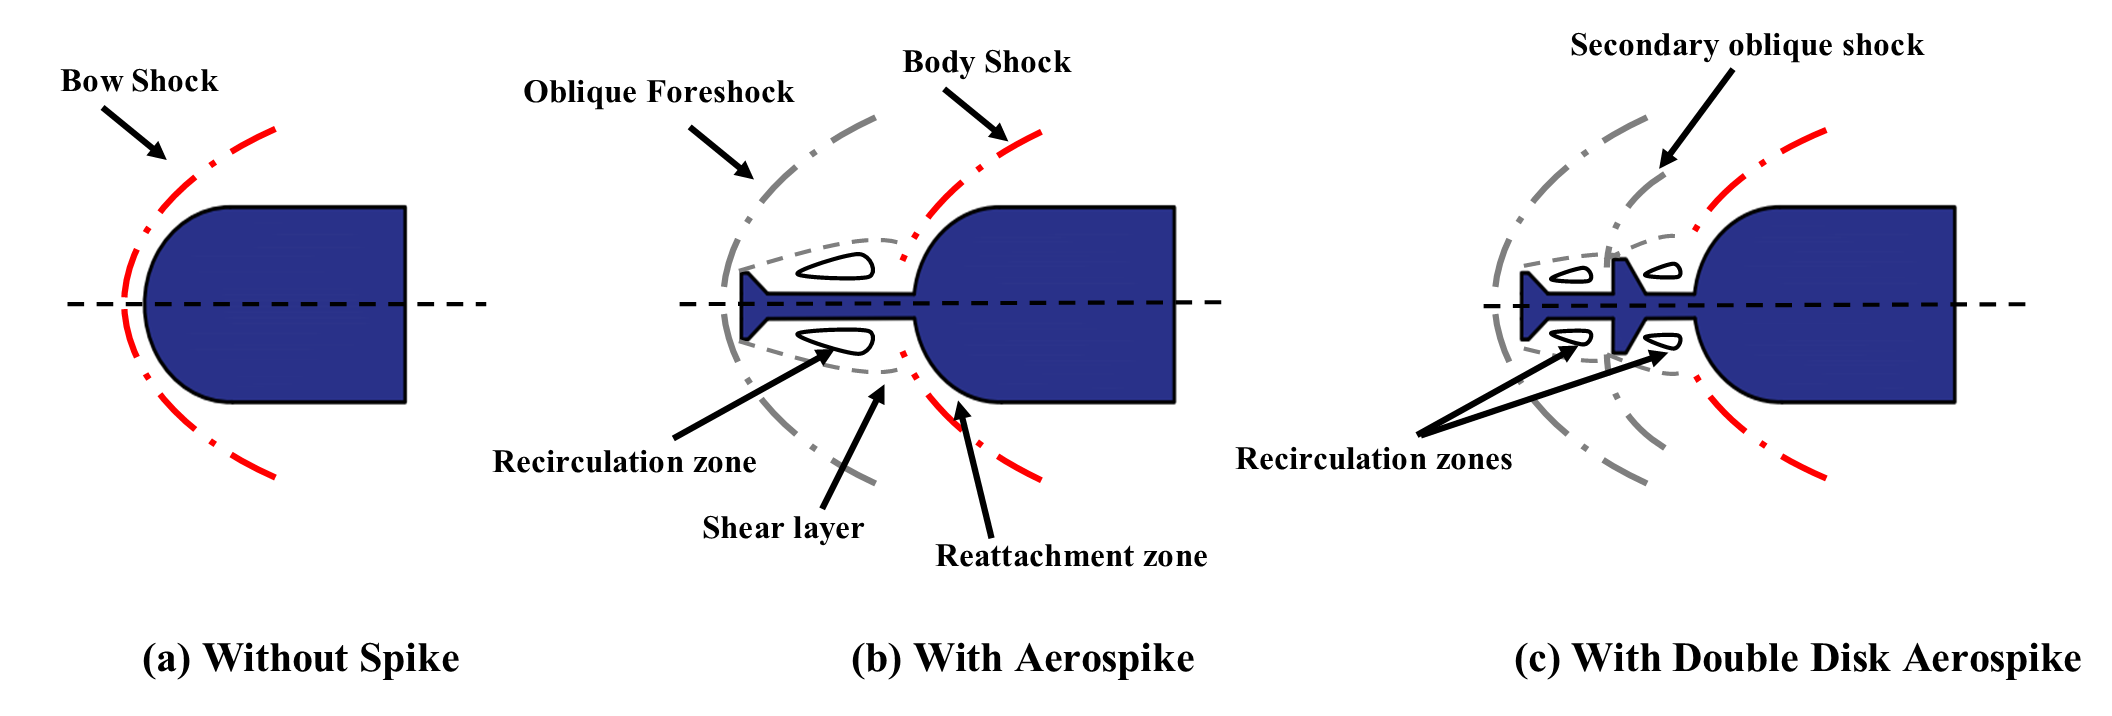
\includegraphics[width=\textwidth]{fig01_schematic.png}
  \caption{Flow topologies compared: (a) clean hemisphere with a detached bow shock; (b) single-disk aerospike with the displaced foreshock, separated shear layer and one dead-air cavity; (c) double-disk aerospike (DDAS), where the second disk splits the dead-air zone into Cavity 1 (between the two disks) and Cavity 2 (between the second disk and the hemisphere).}
  \label{fig:schematic}
\end{figure}

This report uses 2D axisymmetric delayed detached-eddy simulation (DDES) to study the unsteady flow over double-disk aerospikes (DDAS) on a hemisphere at $M_\infty = 2.01$ (Fig.~\ref{fig:schematic}). Seven DDAS cases are built around a pivot case ($l/D = 1.5$, $\dtd = 1.5$, $\ltl = 1$), and one parameter is changed at a time: the disk diameter ratio $\dtd$, the gap ratio $\ltl$ and the spike length $l/D$. A single-disk aerospike (SA) of the same length is the baseline.

The 2D axisymmetric model resolves the dominant streamwise interaction between the shear layer, the shocks and the acoustic waves. It cannot resolve azimuthal instabilities, spanwise deformation of vortices or the 3D turbulent cascade. The $k$--$\omega$ SST model assumes fully turbulent flow. At $Re_D = 2.16\times10^6$ this is a reasonable assumption for the separated shear layer and matches the conditions of the experiments of Sahoo et al.~\cite{Sahoo2020parametric}. The conclusions therefore concern relative changes between configurations rather than absolute values.

The report addresses four questions:
\begin{description}
  \item[RQ1.] How does a second disk change the unsteady flow topology, the spectrum and the loading of a single-disk aerospike at $M_\infty = 2.01$? Does it move spectral energy from a tone to a broad band?
  \item[RQ2.] How does $\dtd$ (1, 1.5, 2) affect the mean and fluctuating pressure at reattachment, the drag and the dominant frequency?
  \item[RQ3.] How does $\ltl$ (0.5, 1, 2) change the coupling between Cavity 1 and Cavity 2, and does it move the flow between pulsation-like and oscillation-like behaviour?
  \item[RQ4.] How does $l/D$ (1, 1.5, 2) set the trade-off between mean drag and unsteadiness, and which parameter has the largest effect overall?
\end{description}

Each case is assessed with: (i) the pressure loading at the reattachment probe, $\zeta = P_\mathrm{rms}/P_\infty$ at $s/D \approx 0.4$, where $P_\mathrm{rms} = \sqrt{\tfrac{1}{n}\sum P_i^2}$ is the root-mean-square of the absolute pressure~\cite{Sahoo2020parametric}; (ii) the fluctuation intensity $\kappa = P_\sigma/P_\mathrm{rms}$ at the same point; (iii) the mean drag coefficient $\Cdm$ and its standard deviation $\sCd$; (iv) the dominant Strouhal number $St = fD/U_\infty$ and the peak premultiplied spectral level $\Pi = fG_{xx}/p_\infty^2$; and (v) the SPOD eigenvalue spectrum $\lambda(St)$~\cite{Schmidt2020guide}.

Section~\ref{sec:method} describes the geometry, the case matrix, the numerical set-up, the time-stepping, the grid and time-step studies and the validation. Section~\ref{sec:results} compares SA with the pivot case and then presents the three parameter sweeps, a cross-case comparison and a combined SPOD analysis. Section~\ref{sec:conclusions} lists the findings.

% ============================================================
\section{Computational methodology}\label{sec:method}

\subsection{Geometry and parameter space}

The body is a hemisphere-cylinder of diameter $D = 50$~mm. A spike of stem diameter $d = 0.12D$ is mounted at the stagnation point. We chose this stem diameter from the Mach 2 experiments of Sahoo et al.~\cite{Sahoo2020parametric}, which tested stem diameters of $0.06D$ and $0.12D$ \chk{CHECK: state their finding on $d/D$ from the paper text}. The primary spike tip is a flat-faced aerodisk of diameter $d_1 = 0.33D$, following the Mach 2 result that a flat aerospike tip gives about 45\% drag reduction against about 30\% for a sharp tip of the same length~\cite{Sahoo2016effect}. The primary disk has an edge thickness $t = 0.0386D$ and a rear conical flare of $130^\circ$ over a length of $0.084D$ (inset of Fig.~\ref{fig:geometry}).

The DDAS adds a coaxial second disk behind the primary disk. It has the same edge thickness and $130^\circ$ flare, so its profile stays the same as its diameter grows. The origin is at the stagnation point of the hemisphere, with $x$ pointing downstream along the axis and $y$ pointing radially outward. The spike tip therefore sits at $x/D = -l/D$.

Three non-dimensional parameters describe the geometry:
\begin{itemize}
  \item $\dtd$, the disk diameter ratio. Earlier work indicates that a second disk smaller than the primary one sits inside the dead-air region and does not intercept the shear layer \chk{SOURCE? the draft cited Yadav and Guven; not found in their abstract}, so we used $\dtd \ge 1$.
  \item $\ltl$, the gap ratio. Here $l_1$ is the axial distance from the primary disk to the second disk and $l_2$ is the distance from the second disk to the stagnation point, with $l = l_1 + l_2$. At fixed $l/D$, a larger $\ltl$ moves the second disk forward, which narrows Cavity 1 and widens Cavity 2: $l_1 = l/(1 + \ltl)$ and $l_2 = l\,(\ltl)/(1 + \ltl)$.
  \item $l/D$, the total spike length ratio. At fixed $\ltl$, $l_1$ and $l_2$ scale with $l$.
\end{itemize}

The pivot case C1 has $l/D = 1.5$, $\dtd = 1.5$ and $\ltl = 1$. Each sweep changes one parameter and holds the other two at the pivot values. The single-disk aerospike SA ($l/D = 1.5$, no second disk) is the reference for drag and spectra. Table~\ref{tab:cases} lists all cases.

\begin{table}[htbp]
  \centering
  \caption{Case matrix. All cases have $d = 0.12D$, $d_1 = 0.33D$ and the pressure probe at $s/D \approx 0.4$ on the hemisphere shoulder ($x/D = 0.152$, $y/D = 0.359$).}
  \label{tab:cases}
  \begin{tabular}{lcccccl}
    \toprule
    Case & $l/D$ & $\ltl$ & $\dtd$ & $l_1/D$ & $l_2/D$ & Sweep \\
    \midrule
    SA & 1.5 & -- & -- & -- & -- & Baseline \\
    C1 & 1.5 & 1.0 & 1.5 & 0.75 & 0.75 & Pivot \\
    C2 & 1.5 & 2.0 & 1.5 & 0.50 & 1.00 & $\ltl$ \\
    C3 & 1.5 & 0.5 & 1.5 & 1.00 & 0.50 & $\ltl$ \\
    C4 & 1.5 & 1.0 & 1.0 & 0.75 & 0.75 & $\dtd$ \\
    C5 & 1.5 & 1.0 & 2.0 & 0.75 & 0.75 & $\dtd$ \\
    C6 & 1.0 & 1.0 & 1.5 & 0.50 & 0.50 & $l/D$ \\
    C7 & 2.0 & 1.0 & 1.5 & 1.00 & 1.00 & $l/D$ \\
    \bottomrule
  \end{tabular}
\end{table}


We recorded unsteady statistics at a fixed probe on the hemisphere shoulder, at $(x/D, y/D) = (0.152, 0.359)$, which is $s/D \approx 0.4$ along the surface. This is the measurement station of Sahoo et al.~\cite{Sahoo2020parametric}, and we kept it at the same physical position in all eight cases. The reattachment point moves with geometry, so in cases where the second disk pushes the shear layer outward (C5, $\dtd = 2$) the probe may not sit exactly at the impingement point. We return to this in the results.

\begin{figure}[htbp]
  \centering
  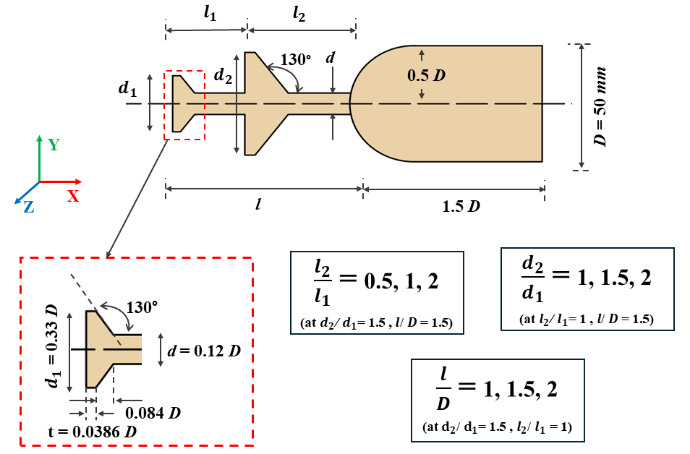
\includegraphics[width=0.7\textwidth]{fig02_geometry.png}
  \caption{DDAS geometry and the three parameters: gap ratio $\ltl$, disk diameter ratio $\dtd$ and spike length $l/D$. The inset (red dashed box) gives the primary disk dimensions. The origin is at the stagnation point of the hemisphere.}
  \label{fig:geometry}
\end{figure}

\subsection{Computational domain and boundary conditions}

The domain is 2D axisymmetric (Fig.~\ref{fig:domain}). It extends $3.75D$ upstream and radially from the stagnation point and $1.5D$ downstream of the hemisphere base, which keeps shock reflections and backflow away from the outer boundaries. The gas is a compressible ideal gas with Sutherland's three-coefficient viscosity law. The freestream boundaries use a pressure far-field condition set to the experimental conditions of Sahoo et al.~\cite{Sahoo2020parametric} (Table~\ref{tab:flow}). The axis has an axisymmetric condition, and all solid surfaces (hemisphere, stem and disks) are adiabatic no-slip walls.

\begin{figure}[htbp]
  \centering
  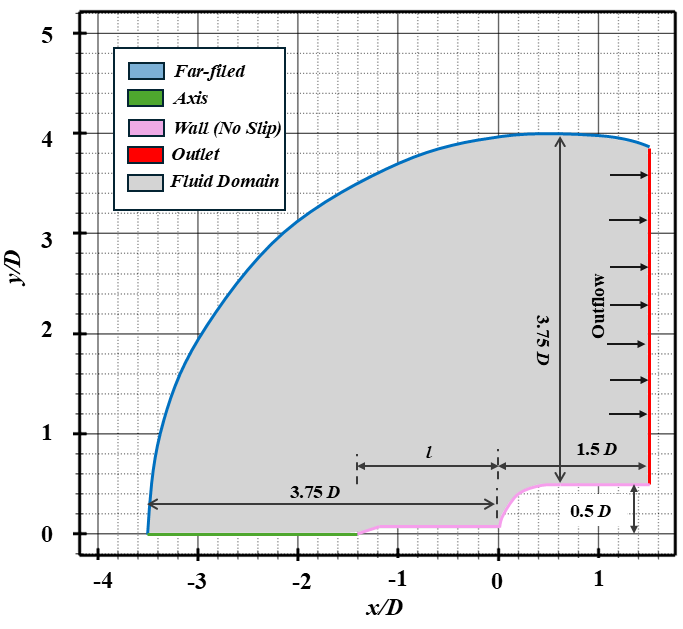
\includegraphics[width=0.5\textwidth]{fig03_domain.png}
  \caption{2D axisymmetric computational domain and boundary types.}
  \label{fig:domain}
\end{figure}

\begin{table}[htbp]
  \centering
  \caption{Freestream and reference conditions.}
  \label{tab:flow}
  \begin{tabular}{lc}
    \toprule
    Parameter & Value \\
    \midrule
    Mach number, $M_\infty$ & 2.01 \\
    Static pressure, $P_\infty$ (Pa) & $0.44\times10^5$ \\
    Static temperature, $T_\infty$ (K) & 163.59 \\
    Velocity, $U_\infty$ (m/s) & 515.15 \\
    Total pressure, $P_0$ (Pa) & $3.48\times10^5$ \\
    Total temperature, $T_0$ (K) & 294.46 \\
    Hemisphere diameter, $D$ (mm) & 50 \\
    Reynolds number, $Re_D = U_\infty D/\nu_\infty$ & $2.16\times10^6$ \\
    Convective time, $T = D/U_\infty$ ($\mu$s) & 97.1 \\
    \bottomrule
  \end{tabular}
\end{table}

\subsection{Numerical method}

We solved the compressible Favre-averaged Navier--Stokes equations with the coupled pressure-based implicit solver of ANSYS Fluent \chk{cite the ANSYS Fluent Theory Guide: not in Zotero, please add}. We used the coupled pressure-based formulation rather than the density-based solver because it converged more stably in a domain that holds both high- and low-Reynolds-number regions \chk{SOURCE? or state as our own experience}. Inlet turbulence was set by an intensity of 5\% and a viscosity ratio of 10.

Gradients used the Green--Gauss node-based method. Convective fluxes used second-order upwind schemes, except momentum, which used bounded central differencing to keep numerical dissipation low in the regions resolved in LES mode. Time integration used a bounded second-order implicit scheme with iterative time advancement.

Turbulence was modelled with DDES built on the $k$--$\omega$ SST model~\cite{Menter1994twoequation}. Near walls the model runs in RANS mode, and in the separated shear layer it switches to an LES-like sub-grid model. In RANS regions the eddy viscosity is
\begin{equation}
  \mu_t = \frac{\rho k}{\max(\omega,\, F_2 S)},
\end{equation}
where $k$ is the turbulent kinetic energy, $\omega$ the specific dissipation rate, $S$ the strain-rate magnitude and $F_2$ the SST blending function \chk{CHECK: Menter's form uses $a_1 k/\max(a_1\omega, SF_2)$}. The DES length scale is
\begin{equation}
  l_\mathrm{DES} = \min\left(l_\mathrm{RANS},\, C_\mathrm{DES}\Delta\right),
\end{equation}
with $l_\mathrm{RANS} = \sqrt{k}/(\beta^*\omega)$, $C_\mathrm{DES}$ a model constant and $\Delta$ the local grid spacing. Where $l_\mathrm{RANS} < C_\mathrm{DES}\Delta$ the model stays in RANS mode, as needed in attached boundary layers. Where the grid is fine enough that $l_\mathrm{RANS} > C_\mathrm{DES}\Delta$, it switches to LES mode and resolves the large eddies of the separated shear layer. The DDES shielding function~\cite{Gritskevich2012development} modifies the destruction term of the $k$ equation so that a fine grid does not switch the boundary layer to LES mode too early:
\begin{center}
  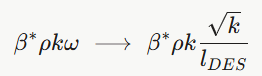
\includegraphics[height=1.1cm]{eq_ddes_shielding.png}
\end{center}

We chose DDES over URANS because URANS damps the large resolved structures of separated shear layers~\cite{Chaouat2017the}, while DES-type models have resolved both feedback modes over spiked bodies~\cite{XUE2018detachededdy}. We chose DDES over wall-resolved LES because LES needs a very fine near-wall grid to resolve the viscous sublayer, whereas DDES keeps RANS resolution there at much lower cost.

\subsection{Time-stepping and data acquisition}\label{sec:timestep}

Figure~\ref{fig:runhistory} shows how each case was run, using C1 as the example. The run started from a hybrid initialisation, which gives a first estimate of the flow from a simplified set of equations in 10 to 20 internal iterations. We then switched on DDES and patched a transverse velocity $v = 0.1U_\infty$ into the shear-layer region to start large-scale oscillations. The flow was then advanced in three phases:
\begin{enumerate}
  \item Phase I, $0 < t < 5$~ms: $\Delta t = 10^{-5}$~s ($\Delta t/T = 0.103$), 500 steps. The coarse step sets up the large-scale oscillation at low cost.
  \item Phase II, $5 < t < 10$~ms: $\Delta t = 10^{-6}$~s ($\Delta t/T = 1.03\times10^{-2}$), 5000 steps. The flow settles into a statistically stationary oscillation.
  \item Phase III, $10 < t < 15$~ms: $\Delta t = 10^{-7}$~s ($\Delta t/T = 1.03\times10^{-3}$, CFL $\approx 1$), 50\,000 steps. All data for post-processing come from this phase.
\end{enumerate}
The total simulated time is 15~ms, or about 154 convective times ($tU_\infty/D$). In Fig.~\ref{fig:runhistory} the probe pressure fluctuates between about 0.5 and 3.5$\pinf$ throughout Phases II and III. The amplitude range does not drift between the two phases, so we take Phase III as stationary.

The 5~ms sampling window of Phase III covers about 51.5 convective times. During this window we exported the flow field from Fluent as ASCII files every 200 time steps (sampling interval $2\times10^{-5}$~s), giving 250 snapshots, and wrote the cell connectivity in CGNS format. The probe pressure and the drag coefficient were written at every time step (50\,000 samples at 10~MHz). The snapshots sample at 50~kHz, so the $x$--$t$, $x$--$f$ and SPOD analyses resolve $St$ up to about 2.43 with a resolution $\Delta St \approx 0.019$. All post-processing used our own MATLAB scripts \chk{the draft cited ref. [82] here; no such reference exists, removed}.

\begin{figure}[htbp]
  \centering
  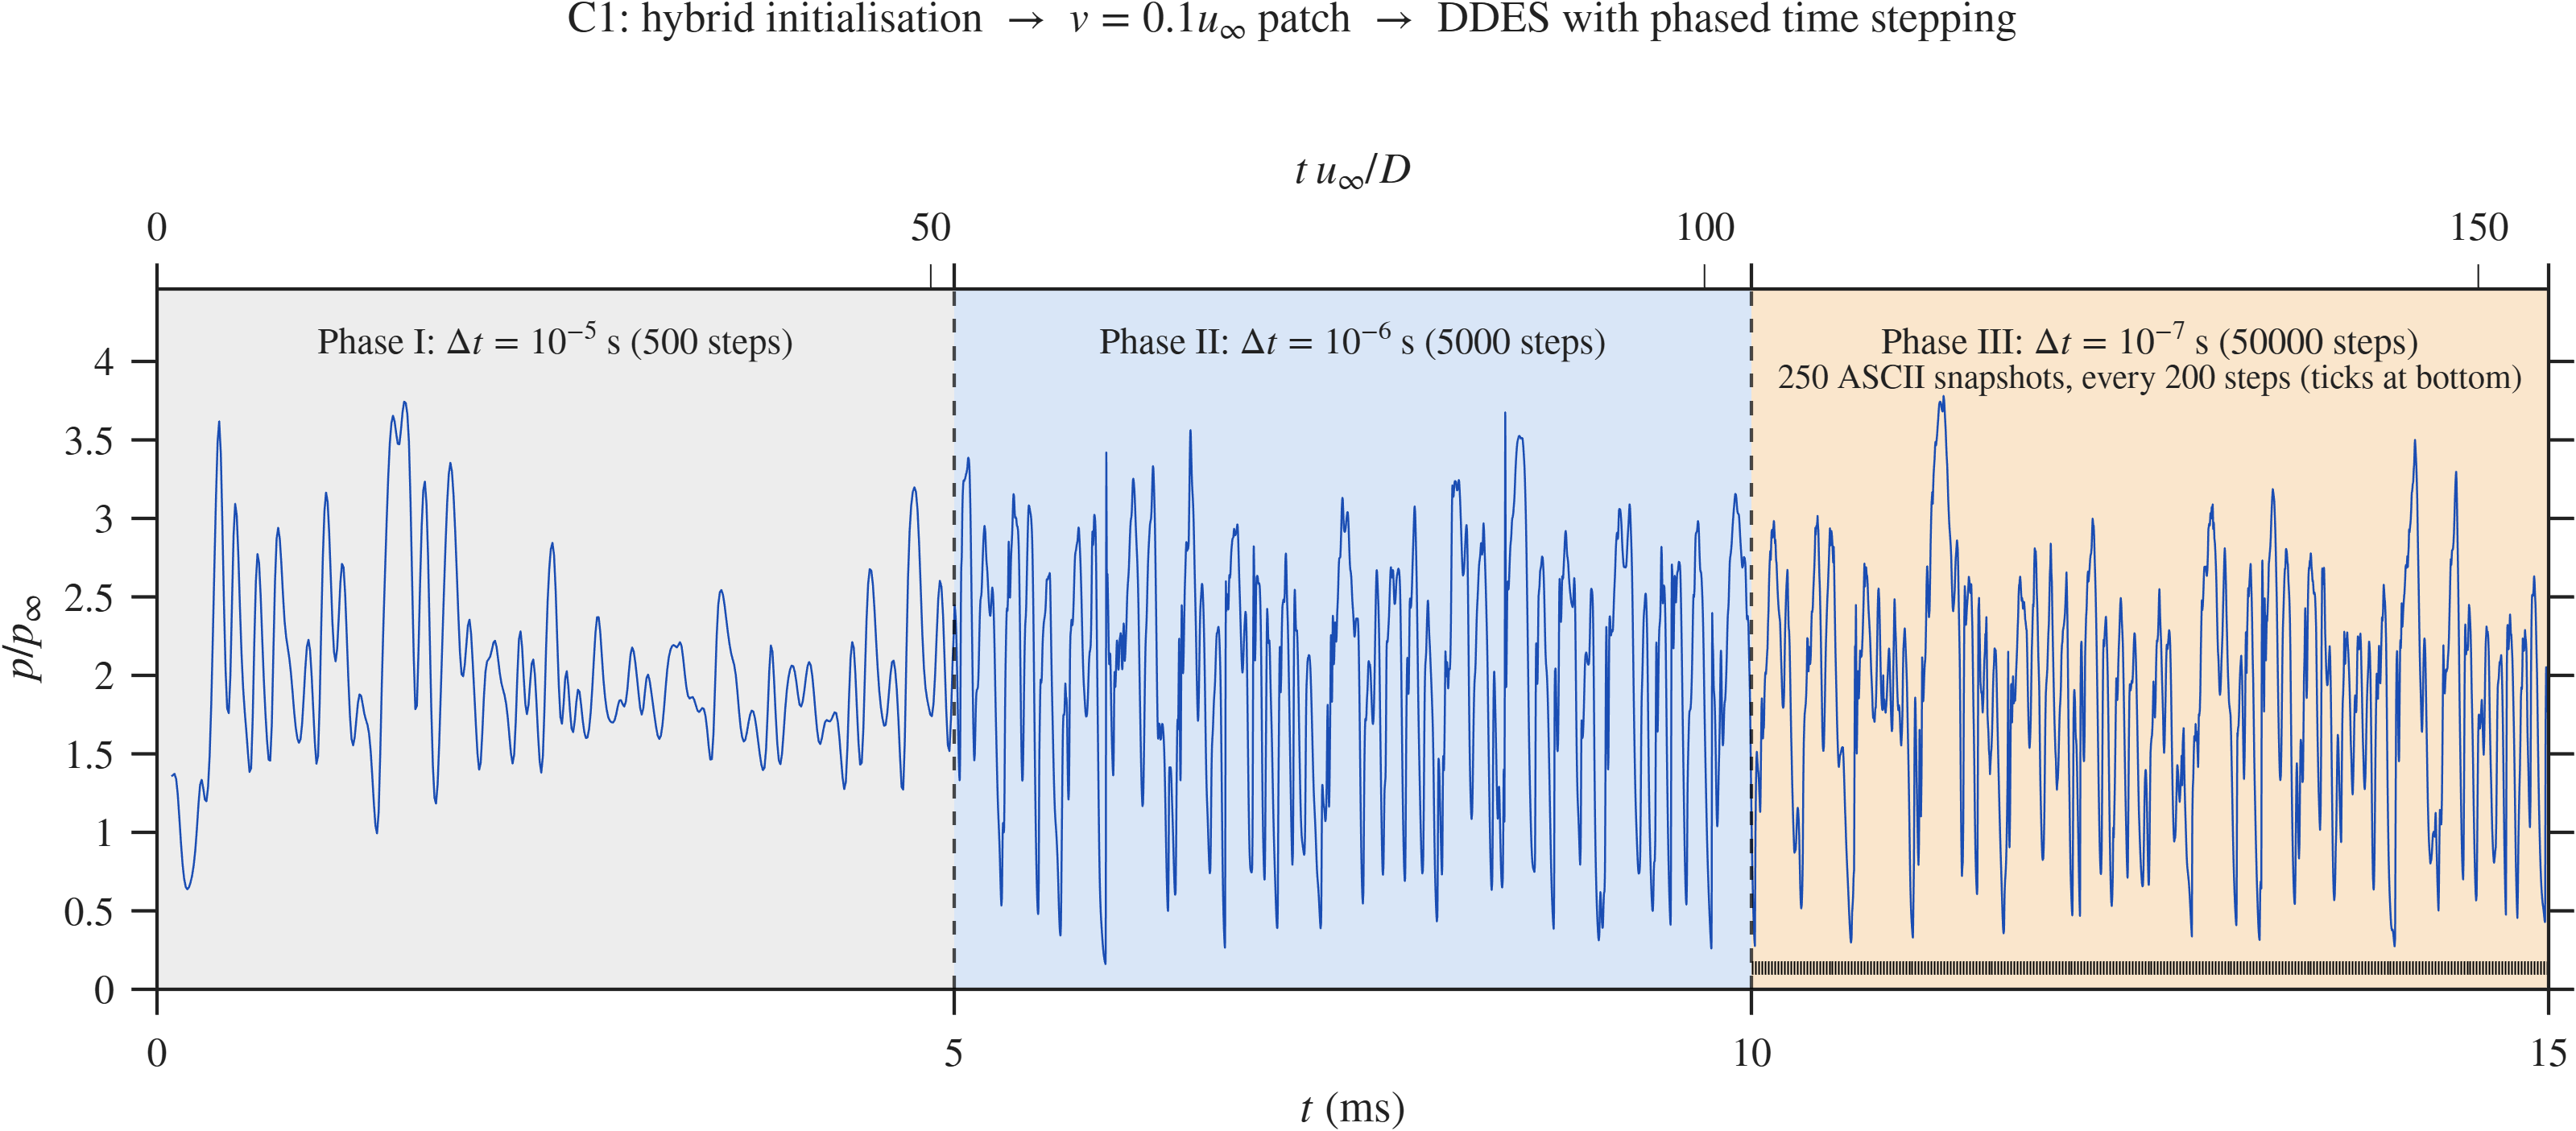
\includegraphics[width=\textwidth]{fig04_C1_run_history.png}
  \caption{Run history of case C1: probe pressure $p/\pinf$ at $s/D \approx 0.4$ against time, after hybrid initialisation and a $v = 0.1u_\infty$ patch. Phase I uses $\Delta t = 10^{-5}$~s (500 steps), Phase II $\Delta t = 10^{-6}$~s (5000 steps) and Phase III $\Delta t = 10^{-7}$~s (50\,000 steps). The ticks at the bottom of Phase III mark the 250 ASCII snapshots (one every 200 steps). All other cases follow the same schedule.}
  \label{fig:runhistory}
\end{figure}

\subsection{Grid and time-step independence}

We tested grid independence with steady RANS on the SA geometry \chk{CHECK: the inset in Fig.~\ref{fig:grid} shows a sharp-tipped spike, i.e. the validation geometry, not SA}. Four multiblock structured grids of about 50\,000, 80\,000, 100\,000 and 130\,000 cells were compared through the mean surface pressure coefficient $C_p$ along the surface arc length $s/D$ (Fig.~\ref{fig:grid}). The three finer grids give the same $C_p$ peak, about 0.69 at $s/D \approx 0.38$, and differ only near $s/D < 0.15$, where the coarse grid lies slightly lower. We used the 130\,000-cell grid for all DDES runs. It keeps $y^+ < 1$ on all walls and has a mean cell skewness of $8.6\times10^{-2}$. Against the experiment, the computed $C_p$ matches the peak value within about 0.03 but falls off faster downstream of $s/D \approx 0.45$.

\begin{figure}[htbp]
  \centering
  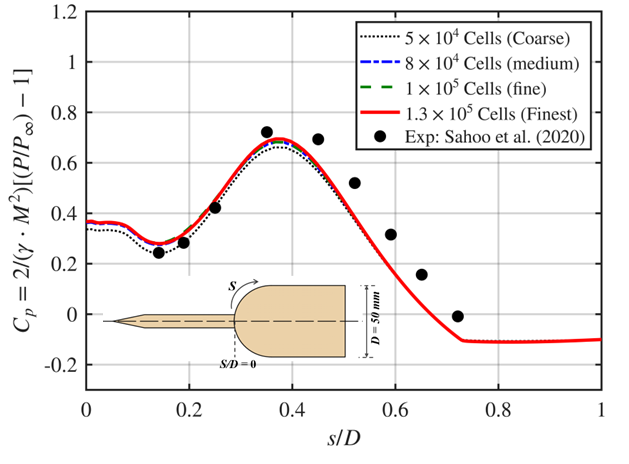
\includegraphics[width=0.6\textwidth]{fig05_grid_Cp.png}
  \caption{Grid independence: mean $C_p$ along the hemisphere surface for four grids, compared with the experiment of Sahoo et al.~\cite{Sahoo2020parametric}.}
  \label{fig:grid}
\end{figure}

We tested the time step with DDES on the same geometry. DDES resolves chaotic eddies in the shear layer, so two runs with different $\Delta t$ do not give the same instantaneous signal, and we judged convergence from statistics over the stationary window. Figure~\ref{fig:dtsignal} shows this: the four signals follow each other for about two convective times after the common start, then separate, while their mean levels (dashed lines) stay close.

We tested four time steps, $\Delta t = 10^{-6}$, $5\times10^{-7}$, $10^{-7}$ and $7.5\times10^{-8}$~s ($\Delta t/T = 1.03\times10^{-2}$, $5.15\times10^{-3}$, $1.03\times10^{-3}$ and $7.72\times10^{-4}$), each over a 5~ms window. Figure~\ref{fig:dt}(a) shows the mean drag coefficient. It falls from 0.423 at $10^{-6}$~s to 0.408 at $10^{-7}$~s and stays at 0.410 at $7.5\times10^{-8}$~s, so the change between the two finest steps is 0.5\%. Figure~\ref{fig:dt}(b) shows the fluctuation intensity $\kappa$ at the probe. It moves from 17.6\% to 17.1\% to 16.2\% and then rises to 19.8\% at the finest step. The error bars of the last three steps overlap, so we read the last rise as sampling scatter within the finite window rather than a trend. We used $\Delta t = 10^{-7}$~s (CFL $\approx 1$) for all cases. It sits on the plateau of both quantities and costs less than the finest step (200 against 267 inner iterations per microsecond).

\begin{figure}[htbp]
  \centering
  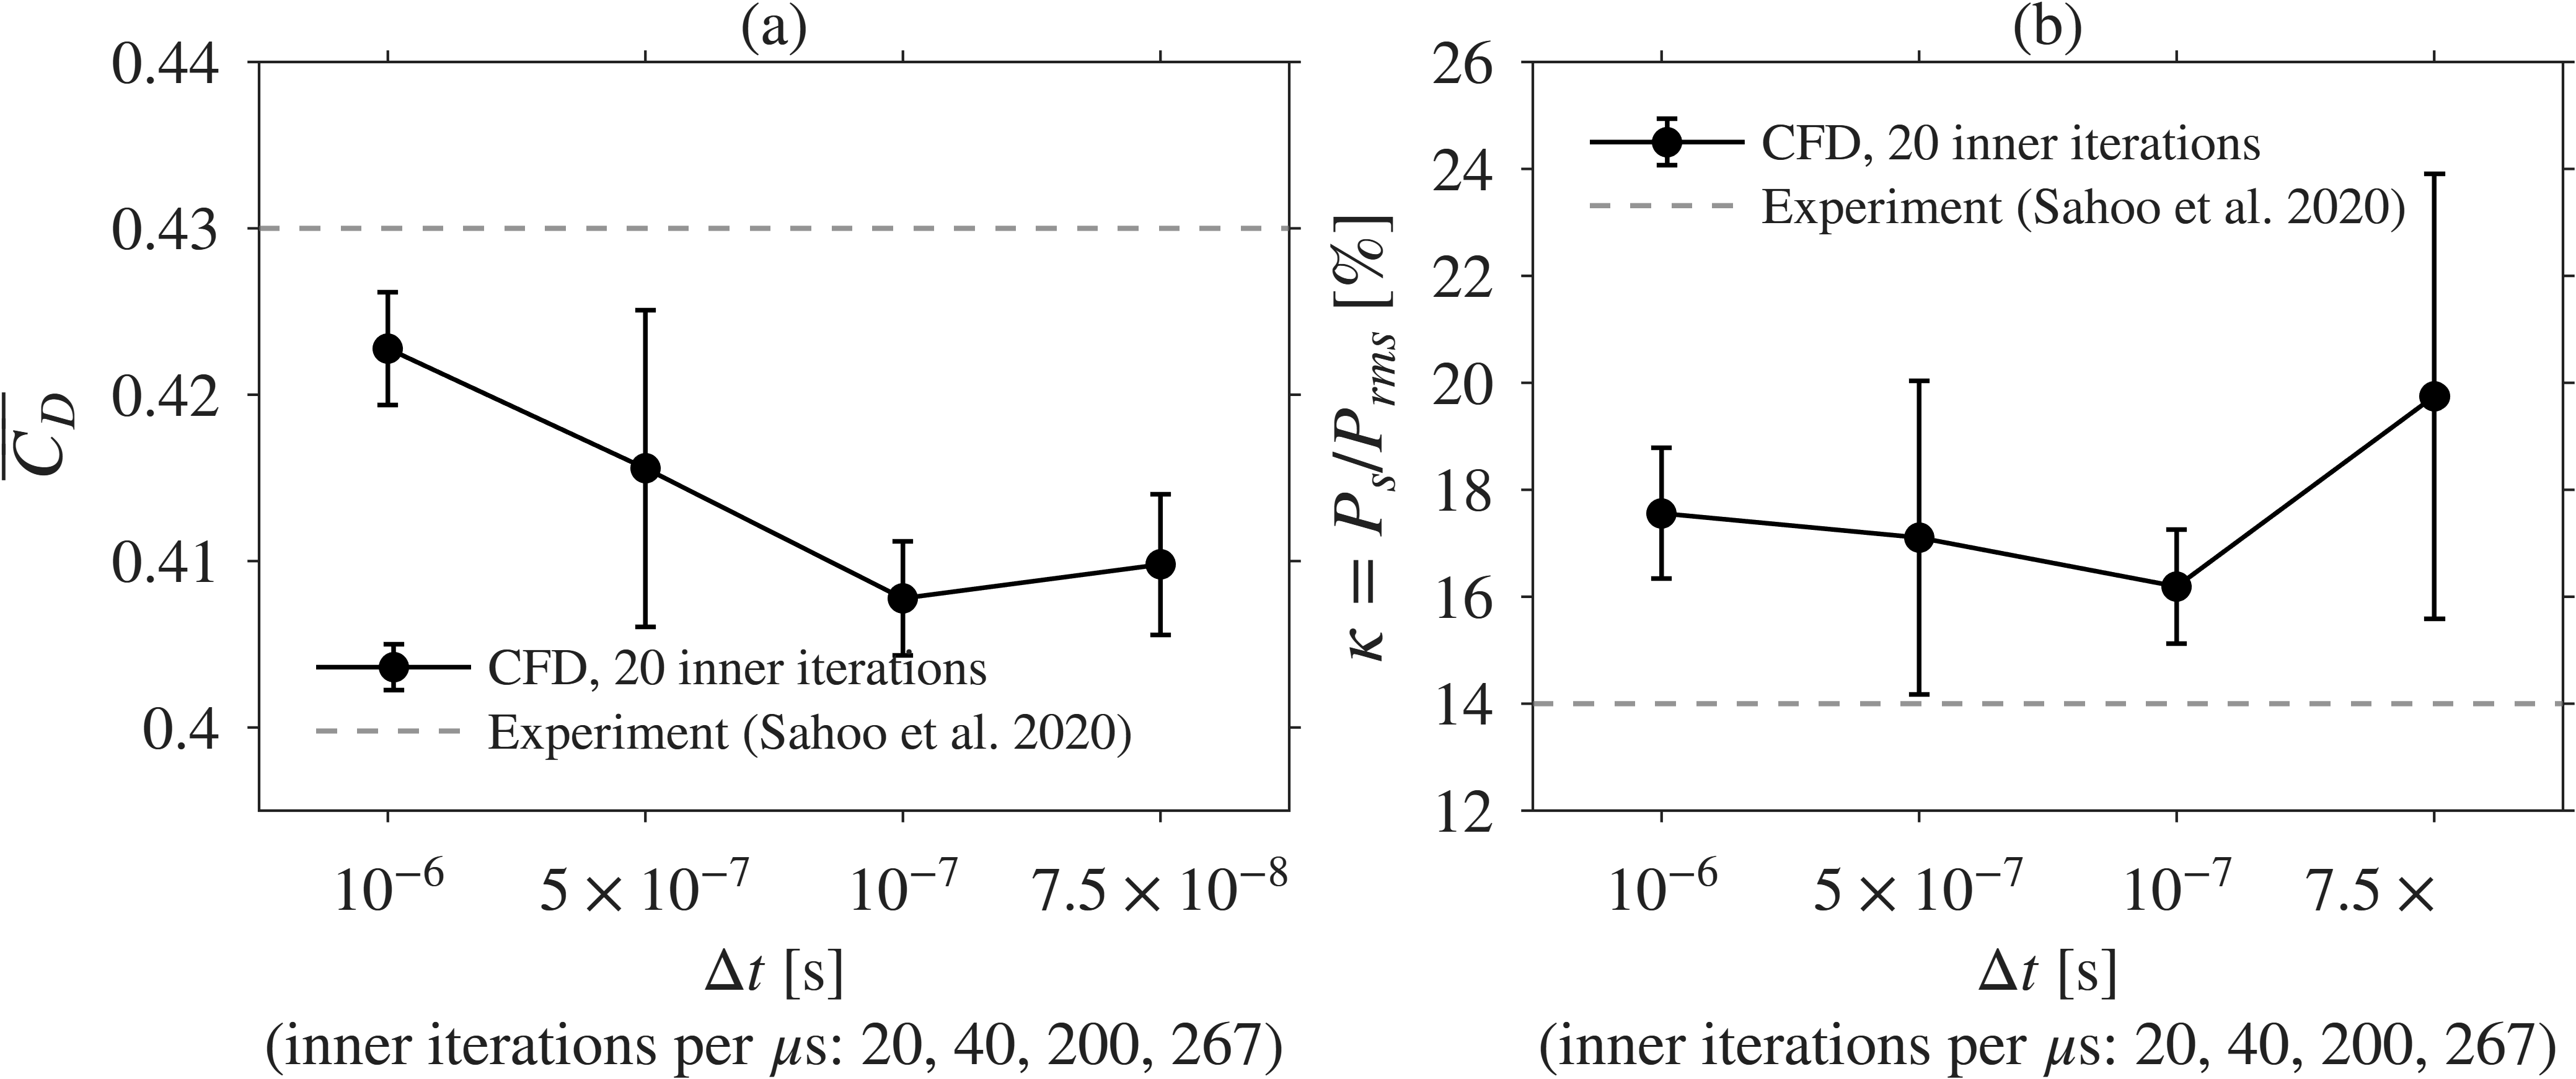
\includegraphics[width=\textwidth]{fig06_timestep_Cd_kappa.png}
  \caption{Time-step independence on the validation geometry: (a) mean drag coefficient $\Cdm$ and (b) fluctuation intensity $\kappa = P_\sigma/P_\mathrm{rms}$ at $s/D \approx 0.4$, for four time steps. Error bars show the scatter over the sampling window. Dashed lines: experiment of Sahoo et al.~\cite{Sahoo2020parametric}.}
  \label{fig:dt}
\end{figure}

\begin{figure}[htbp]
  \centering
  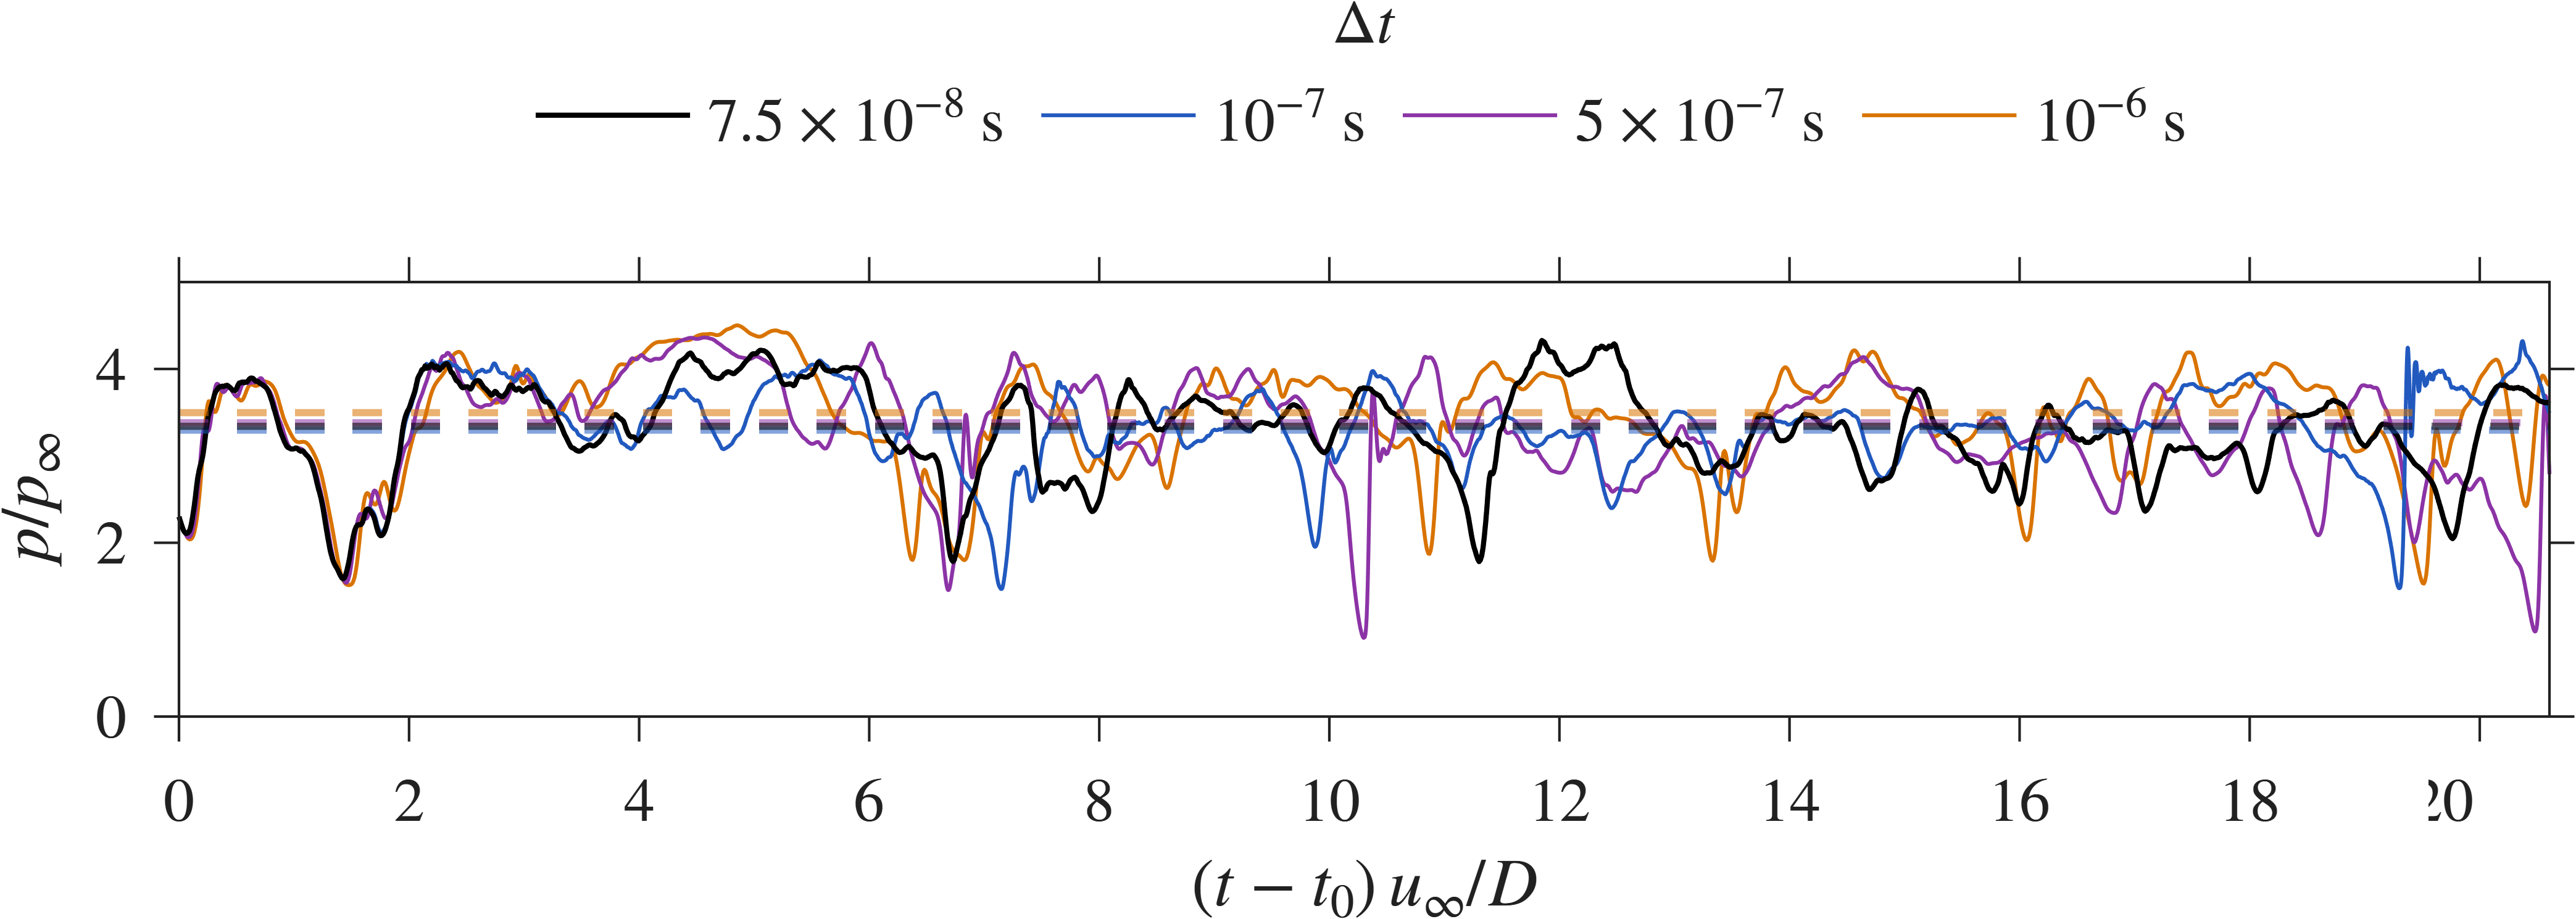
\includegraphics[width=\textwidth]{fig07_timestep_signals.png}
  \caption{Probe pressure $p/\pinf$ at $s/D \approx 0.4$ for the four time steps, from a common start $t_0$. Dashed lines show the mean of each signal.}
  \label{fig:dtsignal}
\end{figure}

\subsection{Validation}

We validated the solver against the wind-tunnel data of Sahoo et al.~\cite{Sahoo2020parametric} for a sharp-tipped spike on the hemisphere ($l/D = 1.5$, $d/D = 0.12$, no aerodisk). This geometry differs from the aerodisk cases of the parameter study, but it uses the same freestream, grid topology, solver settings and turbulence model. It therefore tests whether the method resolves separation, shear-layer roll-up, impingement and the feedback loop at $M_\infty = 2.01$.

We compared three quantities at the probe ($s/D \approx 0.4$). The computed mean drag coefficient is $\Cdm = 0.408$ against 0.43 in the experiment, 5.2\% lower. A 2D axisymmetric model has no circumferential relief, which would let the reattaching flow spread in azimuth, and this is one likely reason for the lower drag. The computed pressure loading is $\zeta = P_\mathrm{rms}/P_\infty = 3.34$ against 2.6 in the experiment, 28.5\% higher. The axisymmetric model forces the whole shear layer to reattach on one ring, which we expect to give a steeper pressure rise than the 3D flow. For this reason the parameter study reports relative changes between cases rather than absolute pressures. The computed fluctuation intensity is $\kappa = 16.2\%$ against 14.0\%, 15.6\% higher. Given the 2D model and the sensitivity of $\kappa$ to the window length and the exact reattachment point, we consider this agreement acceptable for a comparative study.

Figure~\ref{fig:schlieren} compares an instantaneous numerical schlieren ($\partial\rho/\partial x$) with the experimental schlieren~\cite{Sahoo2020parametric}, CFD on the upper half and experiment on the lower half. The foreshock angle, the path of the separated shear layer and the position of the reattachment shock agree. \chk{The draft also discusses the $-5/3$ slope of the validation PSD; that FFT figure is not in the Word file. Add it here as a new figure, or delete this sentence.} The computed probe PSD follows a slope close to $-5/3$ over part of its range. A 2D axisymmetric model has no vortex stretching, so this slope does not prove a resolved turbulent cascade. We read it only as a sign that the scheme is not overly dissipative.

The validation shows that the DDES set-up captures the mean loading, the fluctuation intensity and the dominant shock pattern well enough for a comparative study. The 2D biases (higher $\zeta$, lower $\Cdm$) come from the model and we expect them to affect all configurations in the same direction.

\begin{figure}[htbp]
  \centering
  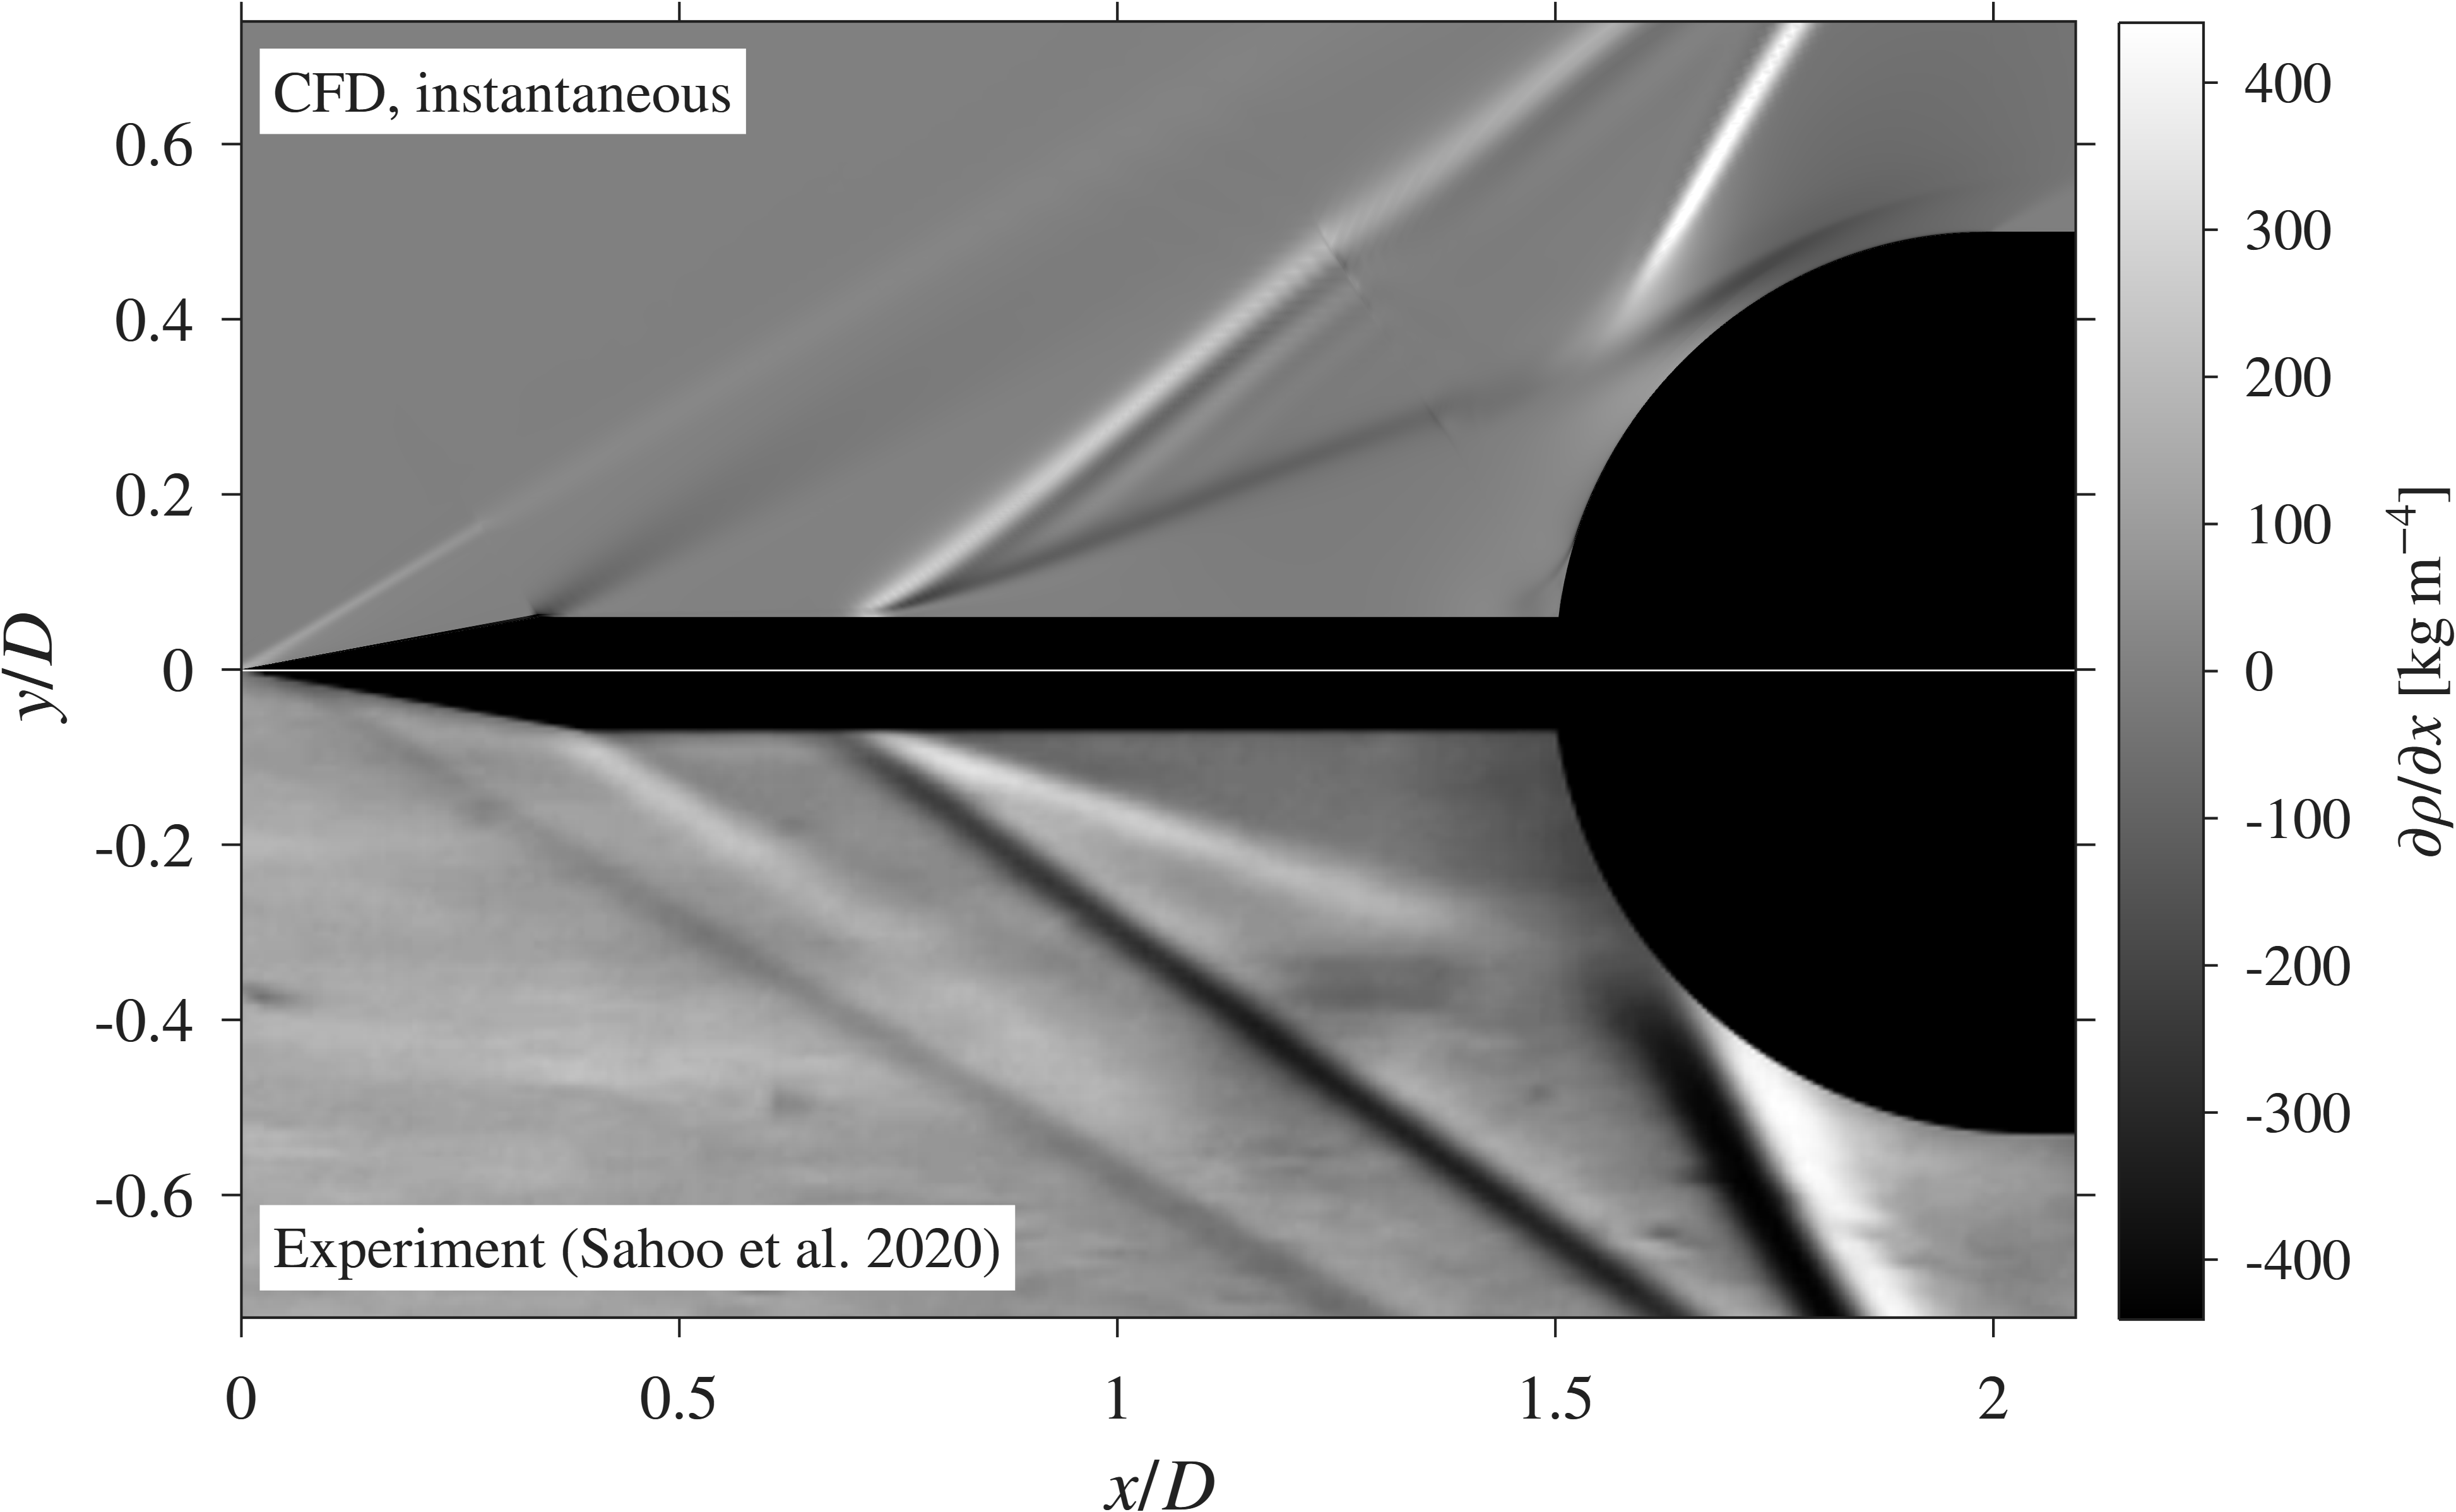
\includegraphics[width=0.85\textwidth]{fig08_schlieren_validation.png}
  \caption{Validation case: instantaneous numerical schlieren $\partial\rho/\partial x$ from DDES (top) and experimental schlieren of Sahoo et al.~\cite{Sahoo2020parametric} (bottom), $M_\infty = 2.01$, sharp spike with $l/D = 1.5$.}
  \label{fig:schlieren}
\end{figure}

% ============================================================
\section{Results and discussion}\label{sec:results}

All statistics come from the 10 to 15~ms window. Contours use the same colour limits in every case ($\pbar$ from 0.4 to 3 and $\psd$ from 0 to 0.9). The $x$--$t$ and $x$--$f$ diagrams use pressure along a probe line 0.8~mm off the stem, disk and hemisphere surfaces. Table~\ref{tab:master} (Section~\ref{sec:synthesis}) collects all the numbers. Values of $\Pi$ and of the SPOD eigenvalue $\lambda_1$ are read from the spectra and are approximate.

% ------------------------------------------------------------
\subsection{Single-disk baseline (SA) against the pivot DDAS (C1)}\label{sec:sa_c1}

This section compares SA with the pivot DDAS C1 ($l/D = 1.5$, $\dtd = 1.5$, $\ltl = 1$) to answer RQ1.

\paragraph{Mean flow.} Figure~\ref{fig:sac1_ms}(a,b) shows the mean pressure with streamlines. In SA the freestream stagnates on the flat face of the disk at $x/D = -1.5$, where $\pbar$ reaches about 3. The flow separates at the disk edge through an expansion fan, and the shear layer encloses one large recirculation vortex between the disk and the hemisphere, where $\pbar < 0.5$. The shear layer reattaches on the shoulder near $x_r/D \approx 0.22$, where a reattachment shock raises the pressure to $\pbar \approx 1.5$ to 2. In C1 the second disk at $x/D = -0.75$ splits the dead-air zone into Cavity 1 ($-1.5 < x/D < -0.75$) and Cavity 2 ($-0.75 < x/D < 0$). Cavity 1 has the lowest pressures ($\pbar < 0.4$), and each cavity holds its own recirculation cell. The reattachment point moves slightly upstream to $x_r/D \approx 0.21$.

\paragraph{Fluctuations.} Figure~\ref{fig:sac1_ms}(c,d) shows $\psd$. In SA the strongest fluctuations ($\psd > 0.8$) sit at the shoulder, where the shear layer strikes the hemisphere. Weaker fluctuations ($\psd \approx 0.2$ to 0.4) run along the shear layer, and the dead-air region and the flow ahead of the disk are almost steady. C1 has three strong regions: (i) the face and edge of the second disk, where the Cavity 1 shear layer strikes; (ii) the inside of Cavity 2; and (iii) the shoulder, which keeps a high level. The fluctuating region of C1 covers both cavities and is larger than in SA.

\begin{figure}[htbp]
  \centering
  \begin{subfigure}{0.49\textwidth}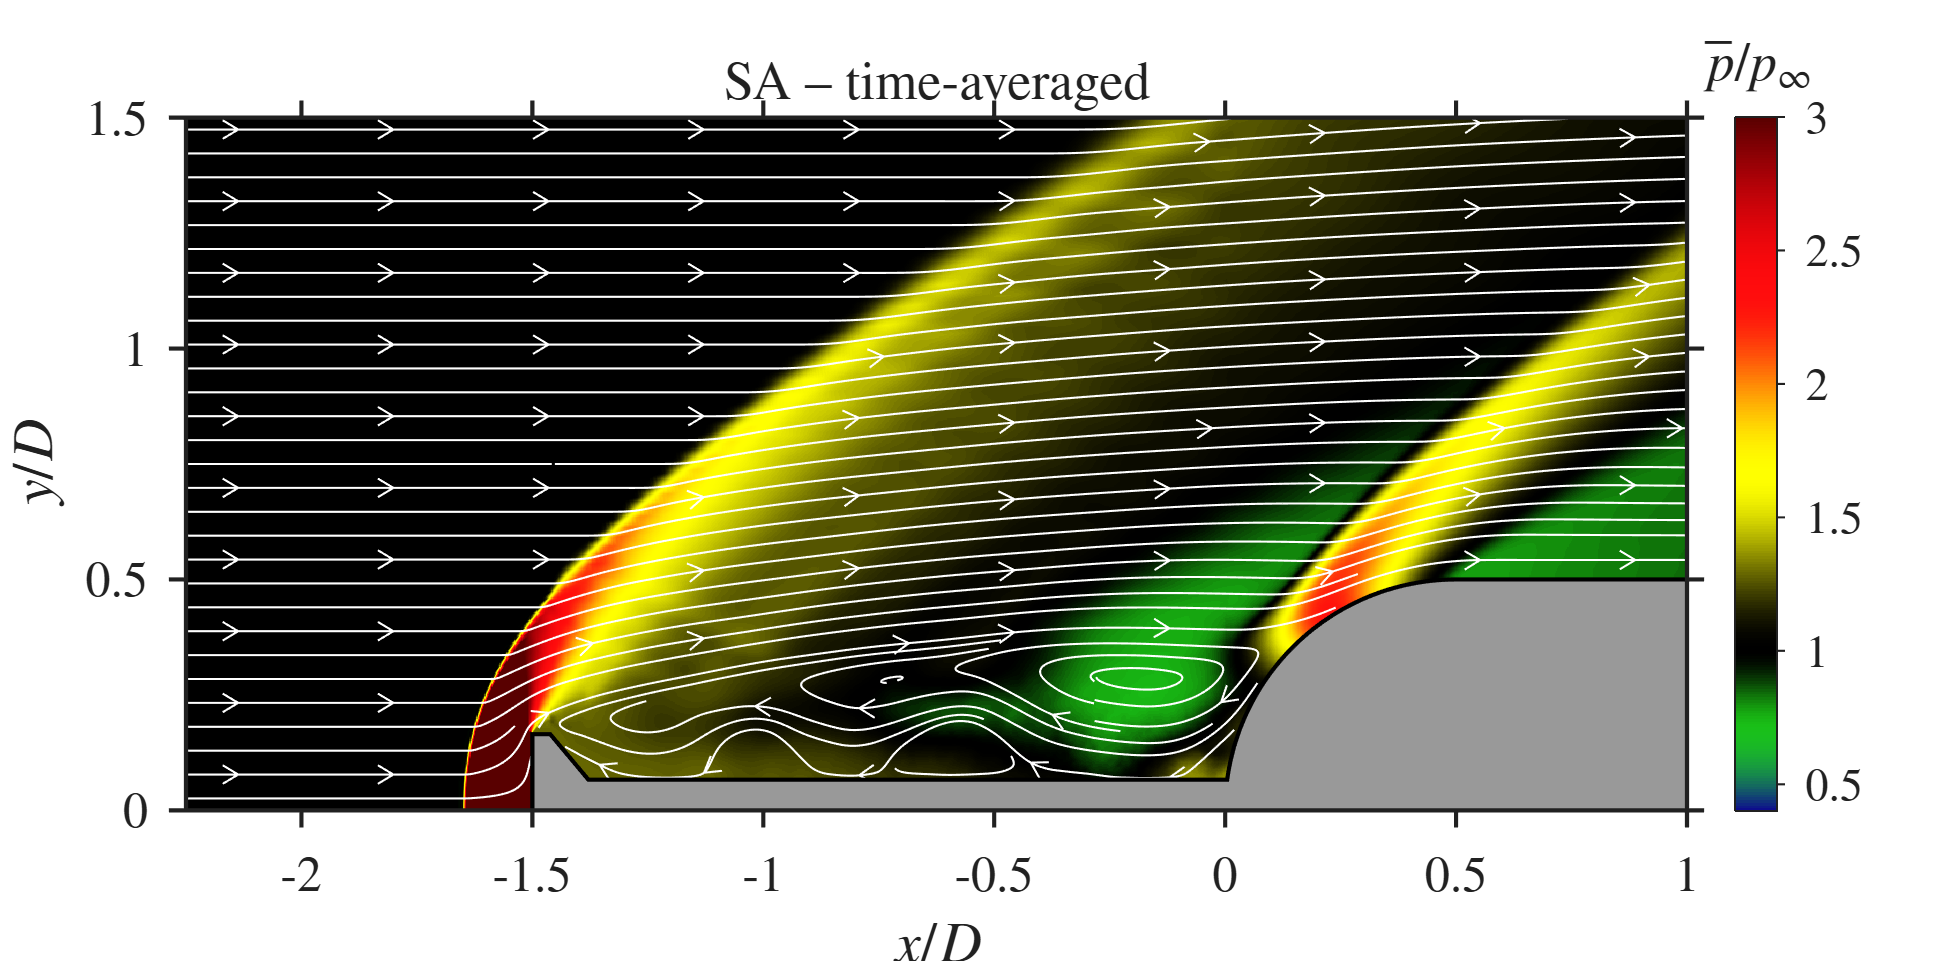
\includegraphics[width=\linewidth]{SA_mean.png}\caption{SA, $\pbar$}\end{subfigure}
  \begin{subfigure}{0.49\textwidth}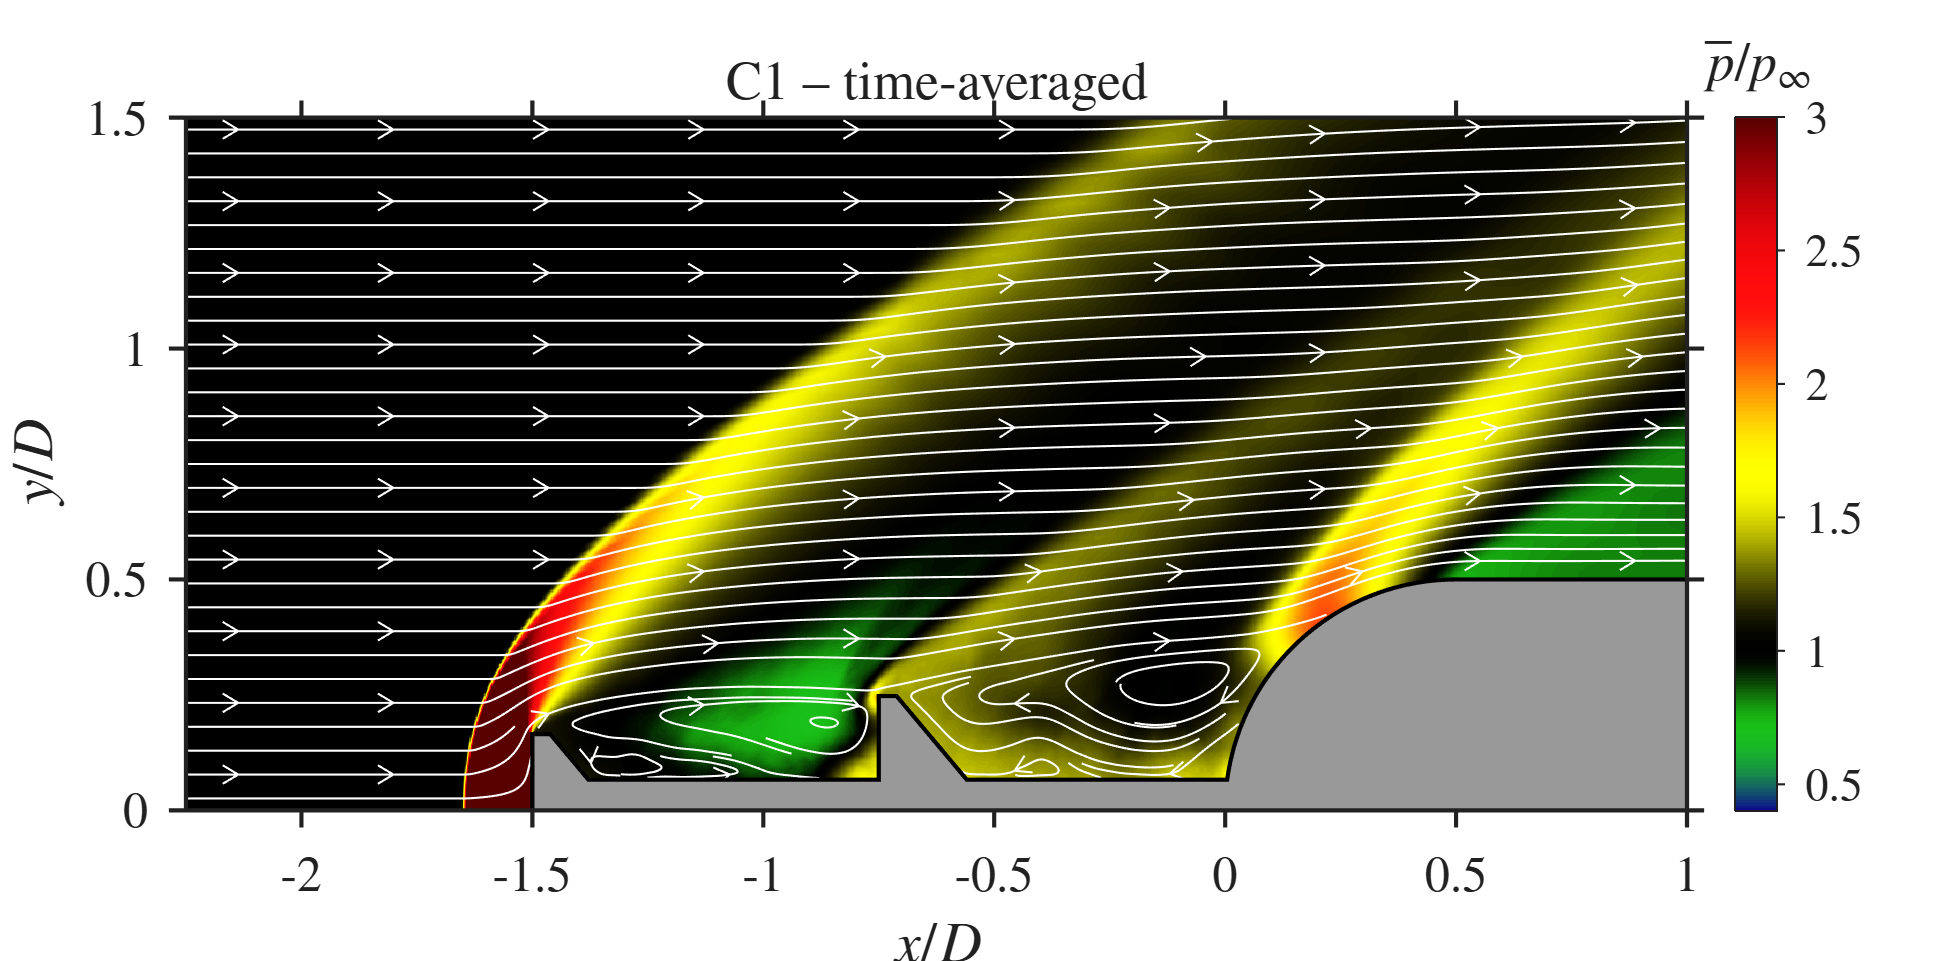
\includegraphics[width=\linewidth]{C1_mean.png}\caption{C1, $\pbar$}\end{subfigure}\\[2pt]
  \begin{subfigure}{0.49\textwidth}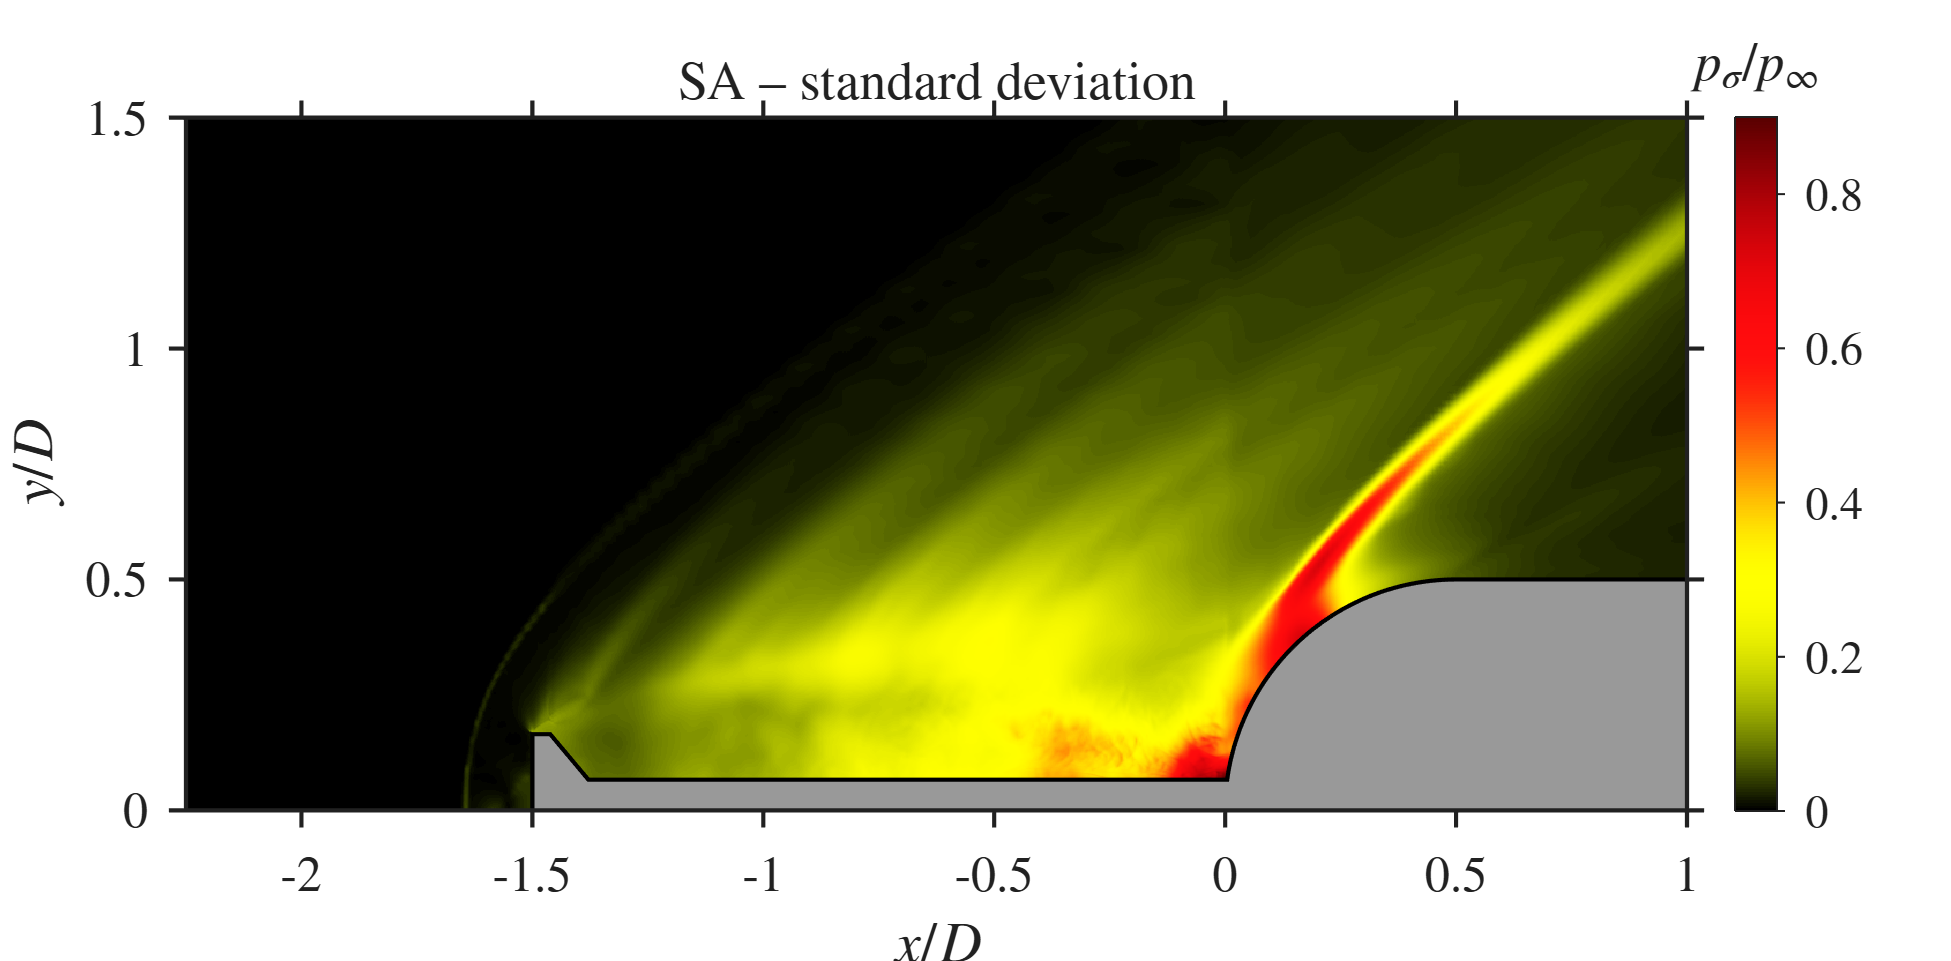
\includegraphics[width=\linewidth]{SA_std.png}\caption{SA, $\psd$}\end{subfigure}
  \begin{subfigure}{0.49\textwidth}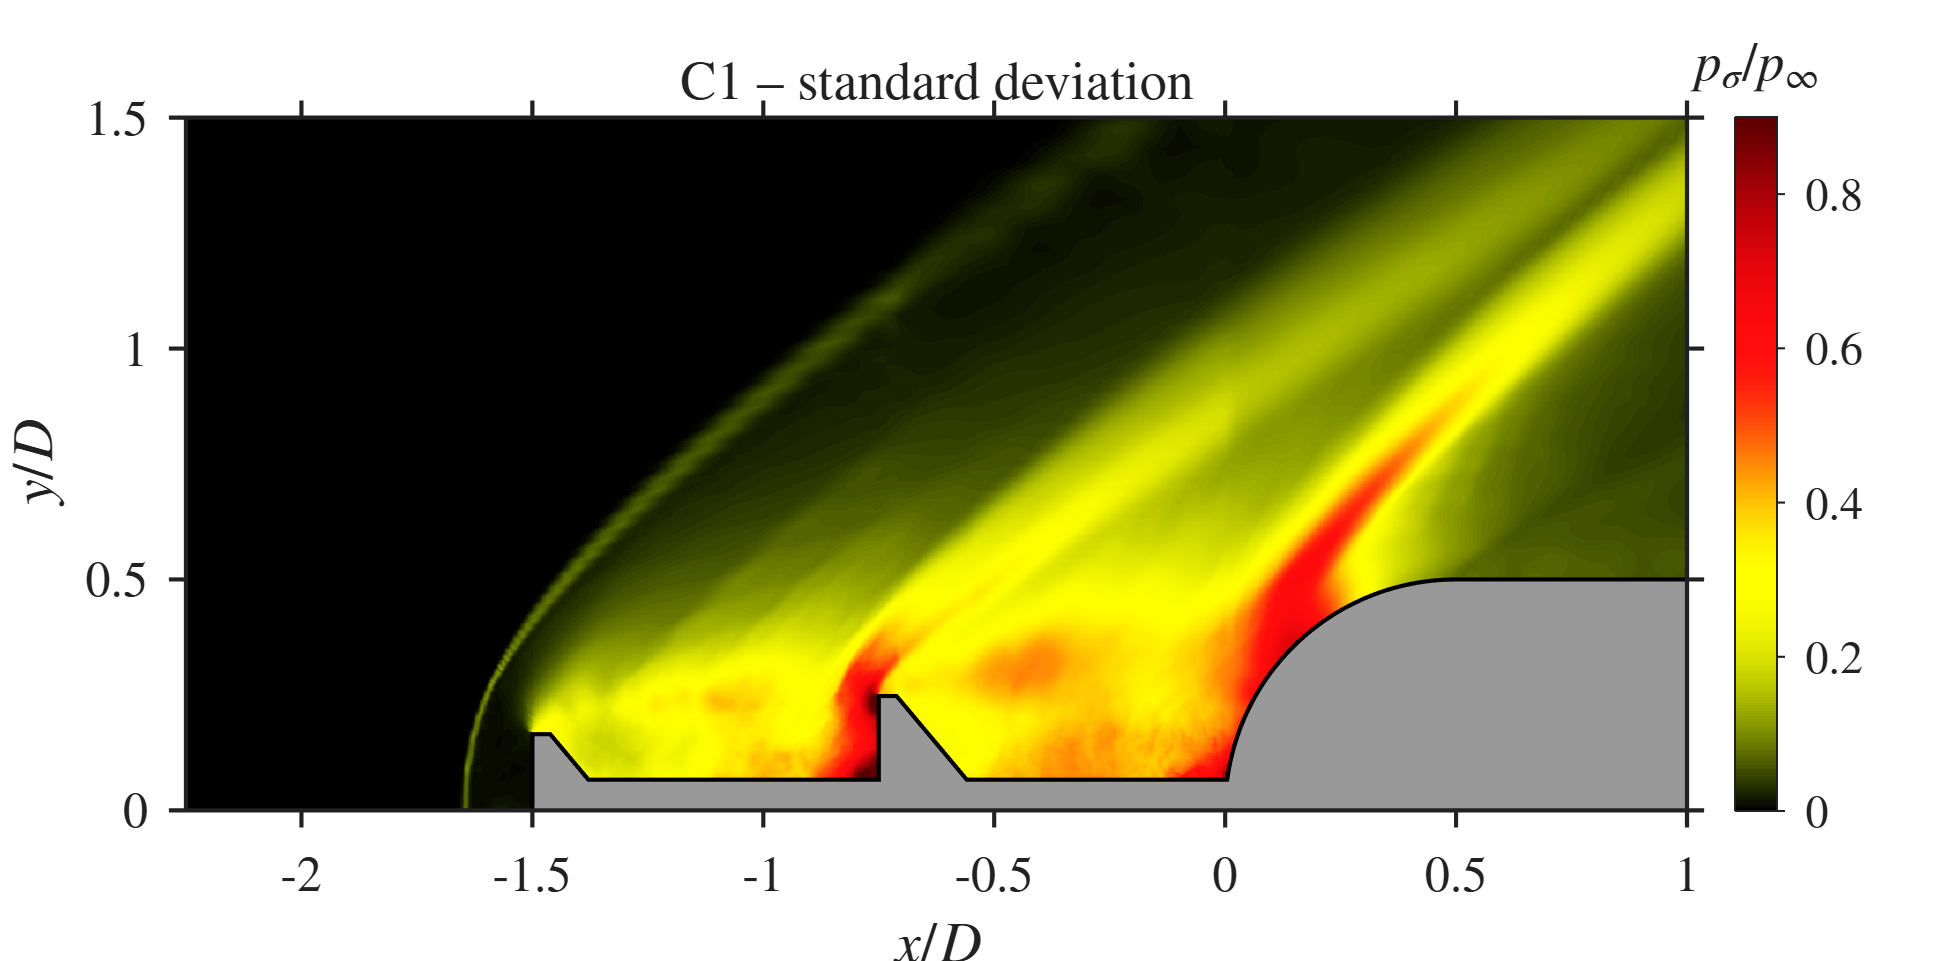
\includegraphics[width=\linewidth]{C1_std.png}\caption{C1, $\psd$}\end{subfigure}
  \caption{Mean pressure with streamlines (top) and pressure standard deviation (bottom) for SA and C1.}
  \label{fig:sac1_ms}
\end{figure}

\paragraph{Space-time behaviour.} Figure~\ref{fig:sac1_xt} shows the $x$--$t$ diagrams. In SA, diagonal streaks run from the disk ($x/D \approx -1.5$) toward the reattachment line ($x_r/D = 0.218$). These are vortical structures convecting down the shear layer. At the reattachment line, high- and low-pressure bands alternate with a period of about $1.3D/U_\infty$, which corresponds to $St \approx 0.76$. In C1 the second disk appears as a gap in the probe line and splits the diagram into two parts. Cavity 1 shows irregular high-pressure bursts instead of regular streaks, and Cavity 2 shows several time scales at once. The reattachment line ($x_r/D = 0.207$) still alternates between high and low pressure, but the period is less regular.

\begin{figure}[htbp]
  \centering
  \begin{subfigure}{0.48\textwidth}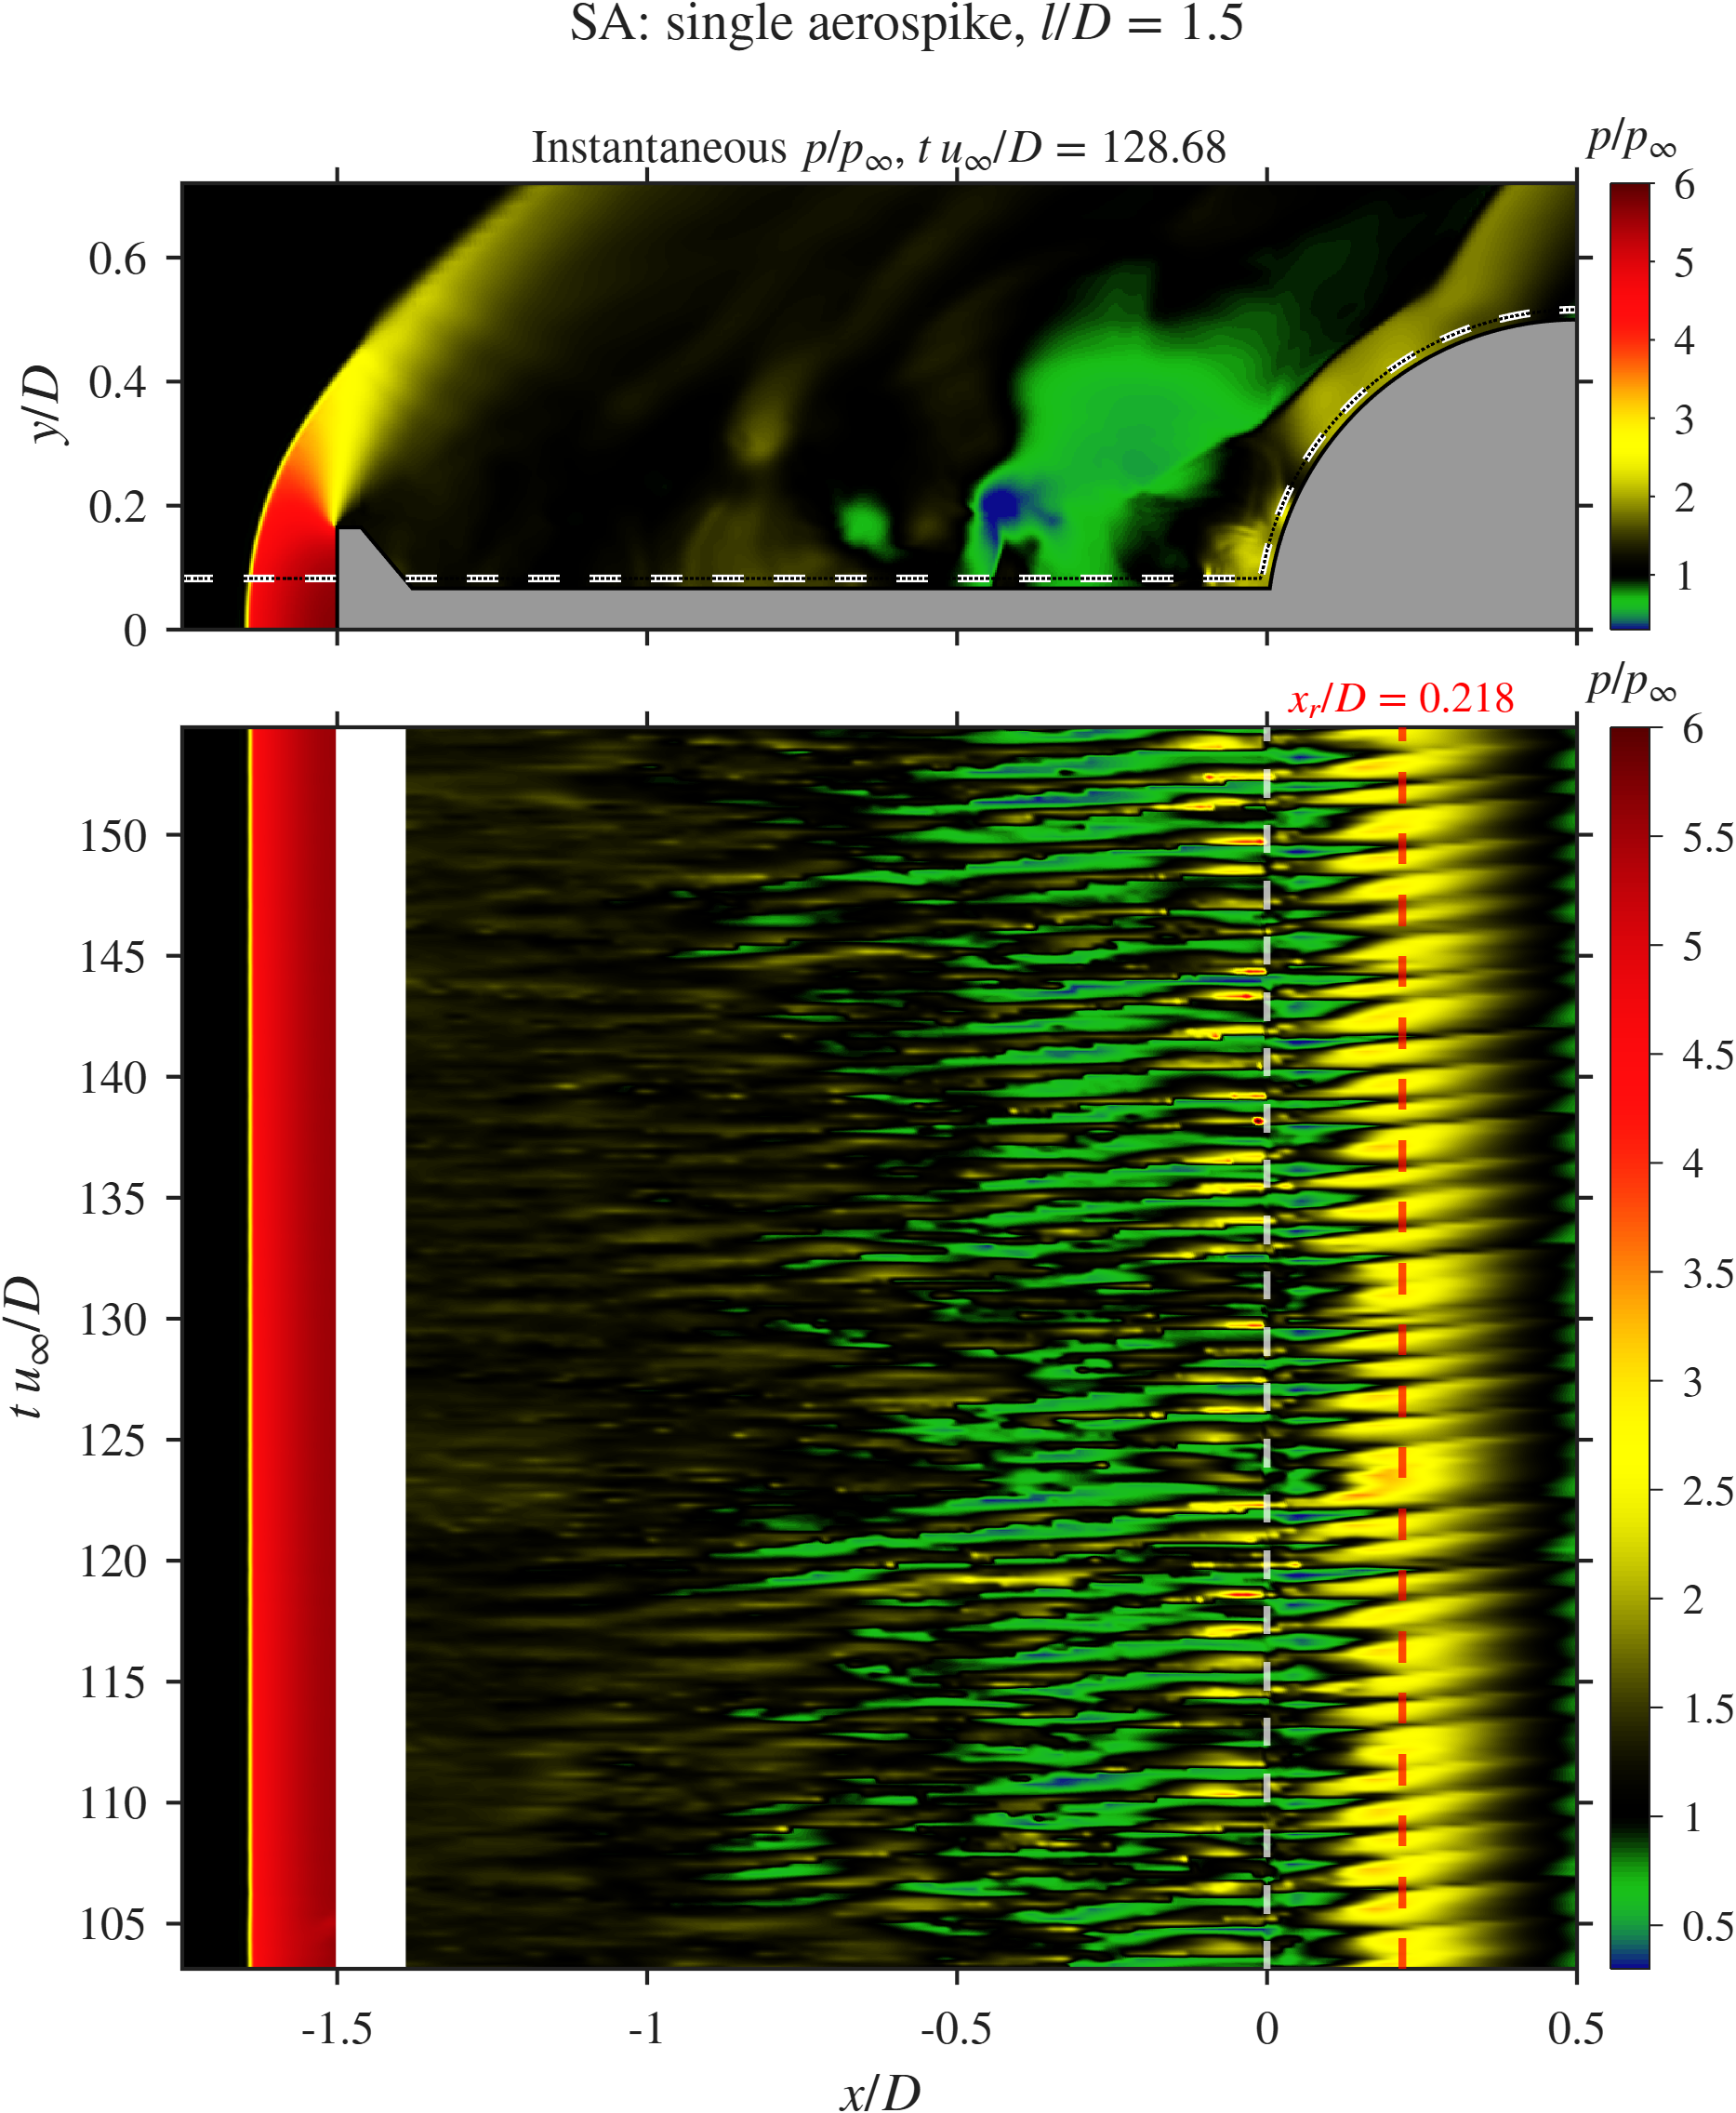
\includegraphics[width=\linewidth]{SA_xt.png}\caption{SA}\end{subfigure}
  \begin{subfigure}{0.48\textwidth}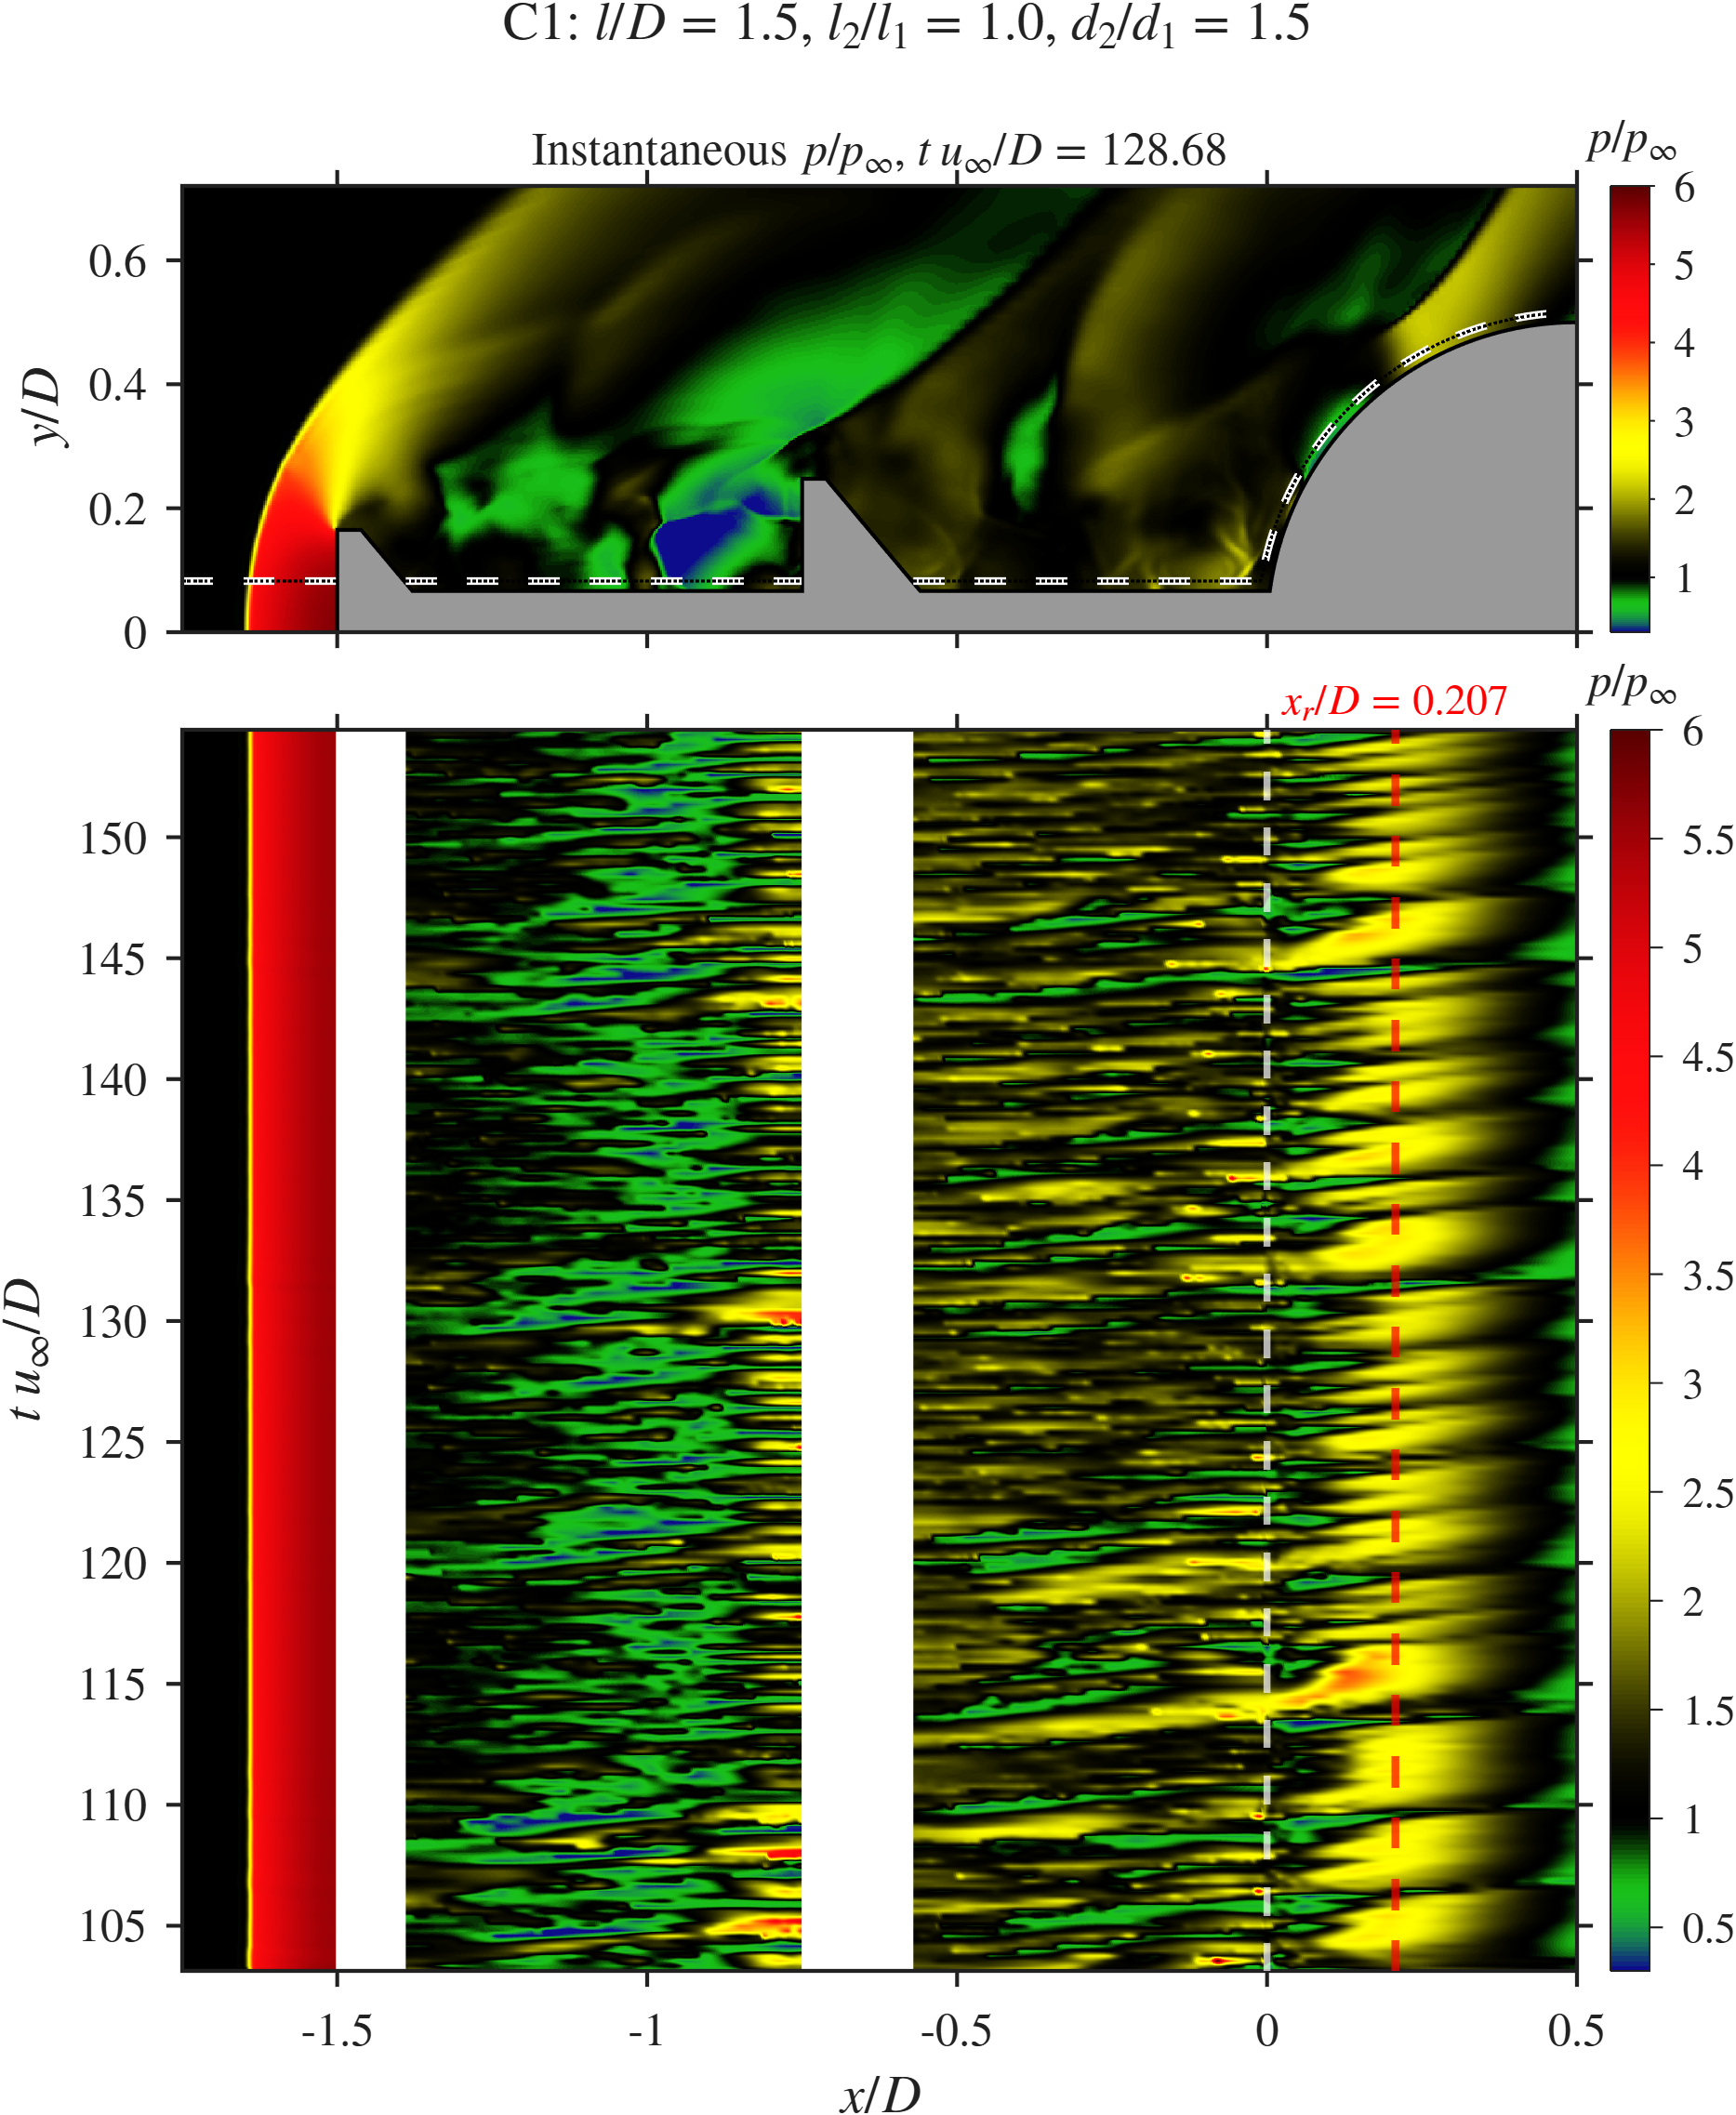
\includegraphics[width=\linewidth]{C1_xt.png}\caption{C1}\end{subfigure}
  \caption{$x$--$t$ diagrams of $p/\pinf$ along the probe line for SA and C1 (top panels: instantaneous field with the probe line dashed). The red dashed line marks the reattachment point $x_r$.}
  \label{fig:sac1_xt}
\end{figure}

Figure~\ref{fig:sac1_xf} shows where along the probe line each frequency lives. In SA one band at $St \approx 0.76$ runs along the whole line, strongest near the reattachment point. In C1 the energy splits by cavity: a band at $St \approx 1.14$ sits at the face of the second disk, and a weaker band at $St \approx 0.68$ sits in Cavity 2 and at the shoulder.

\begin{figure}[htbp]
  \centering
  \begin{subfigure}{0.48\textwidth}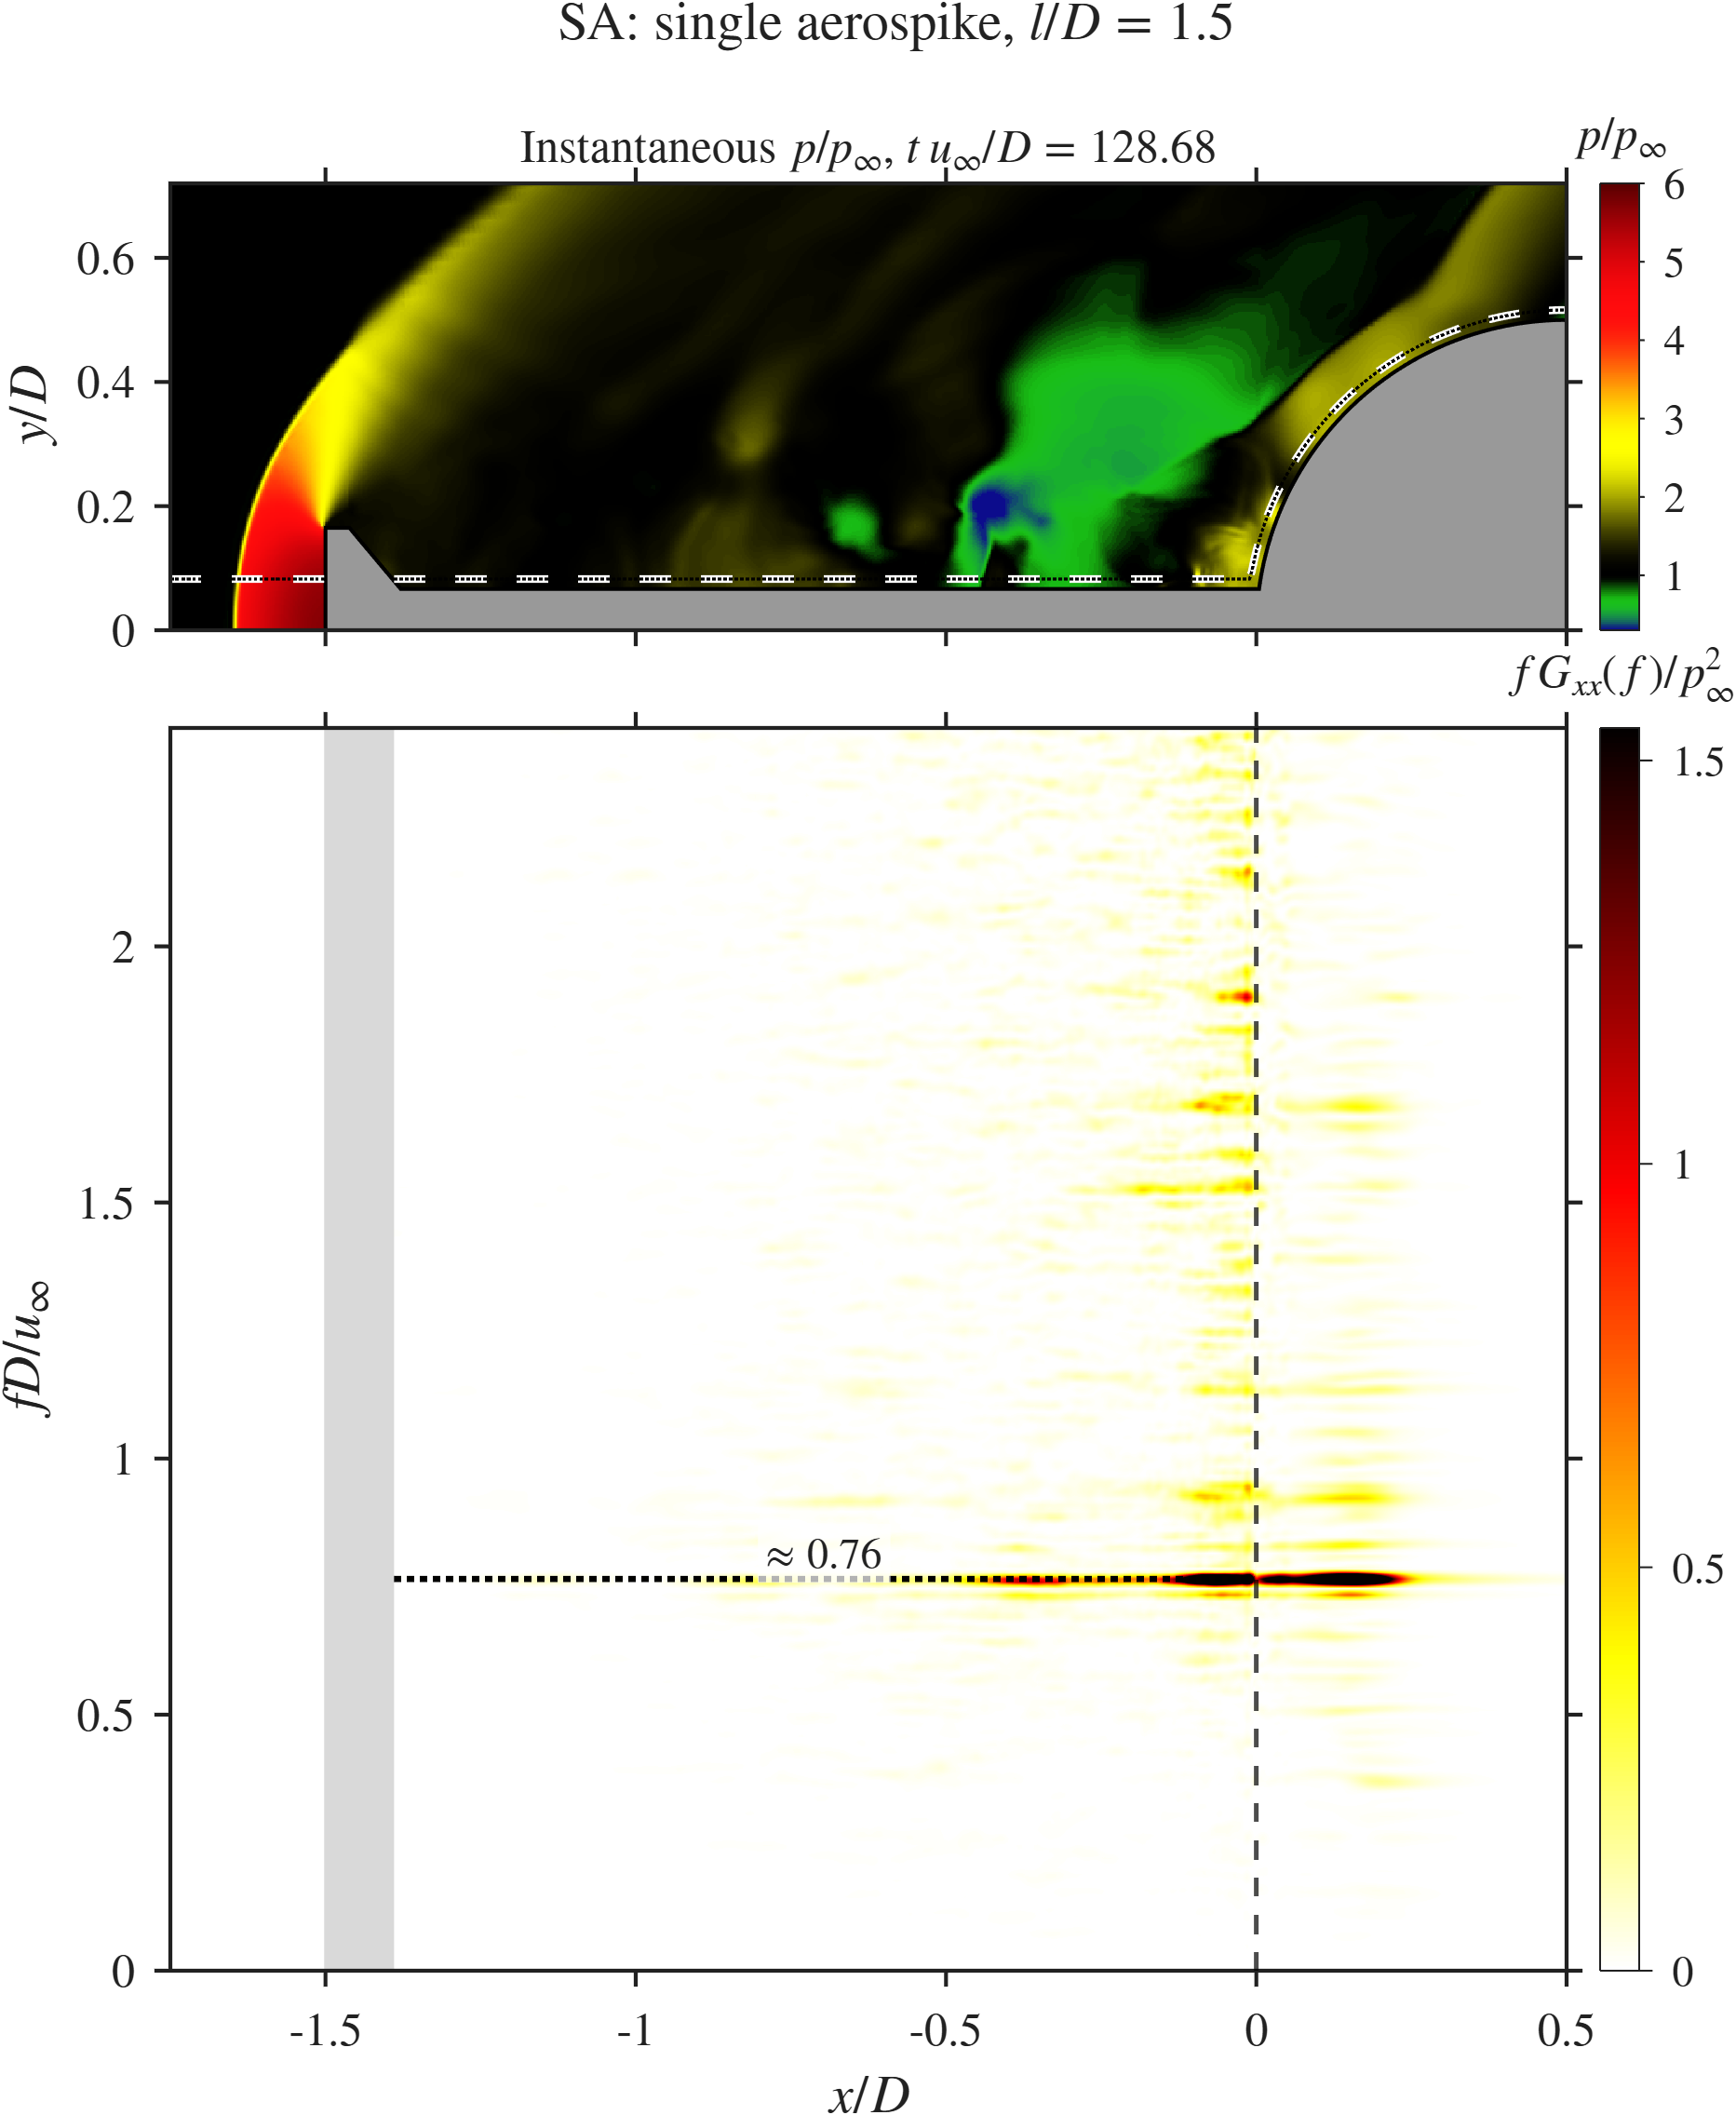
\includegraphics[width=\linewidth]{SA_xf.png}\caption{SA}\end{subfigure}
  \begin{subfigure}{0.48\textwidth}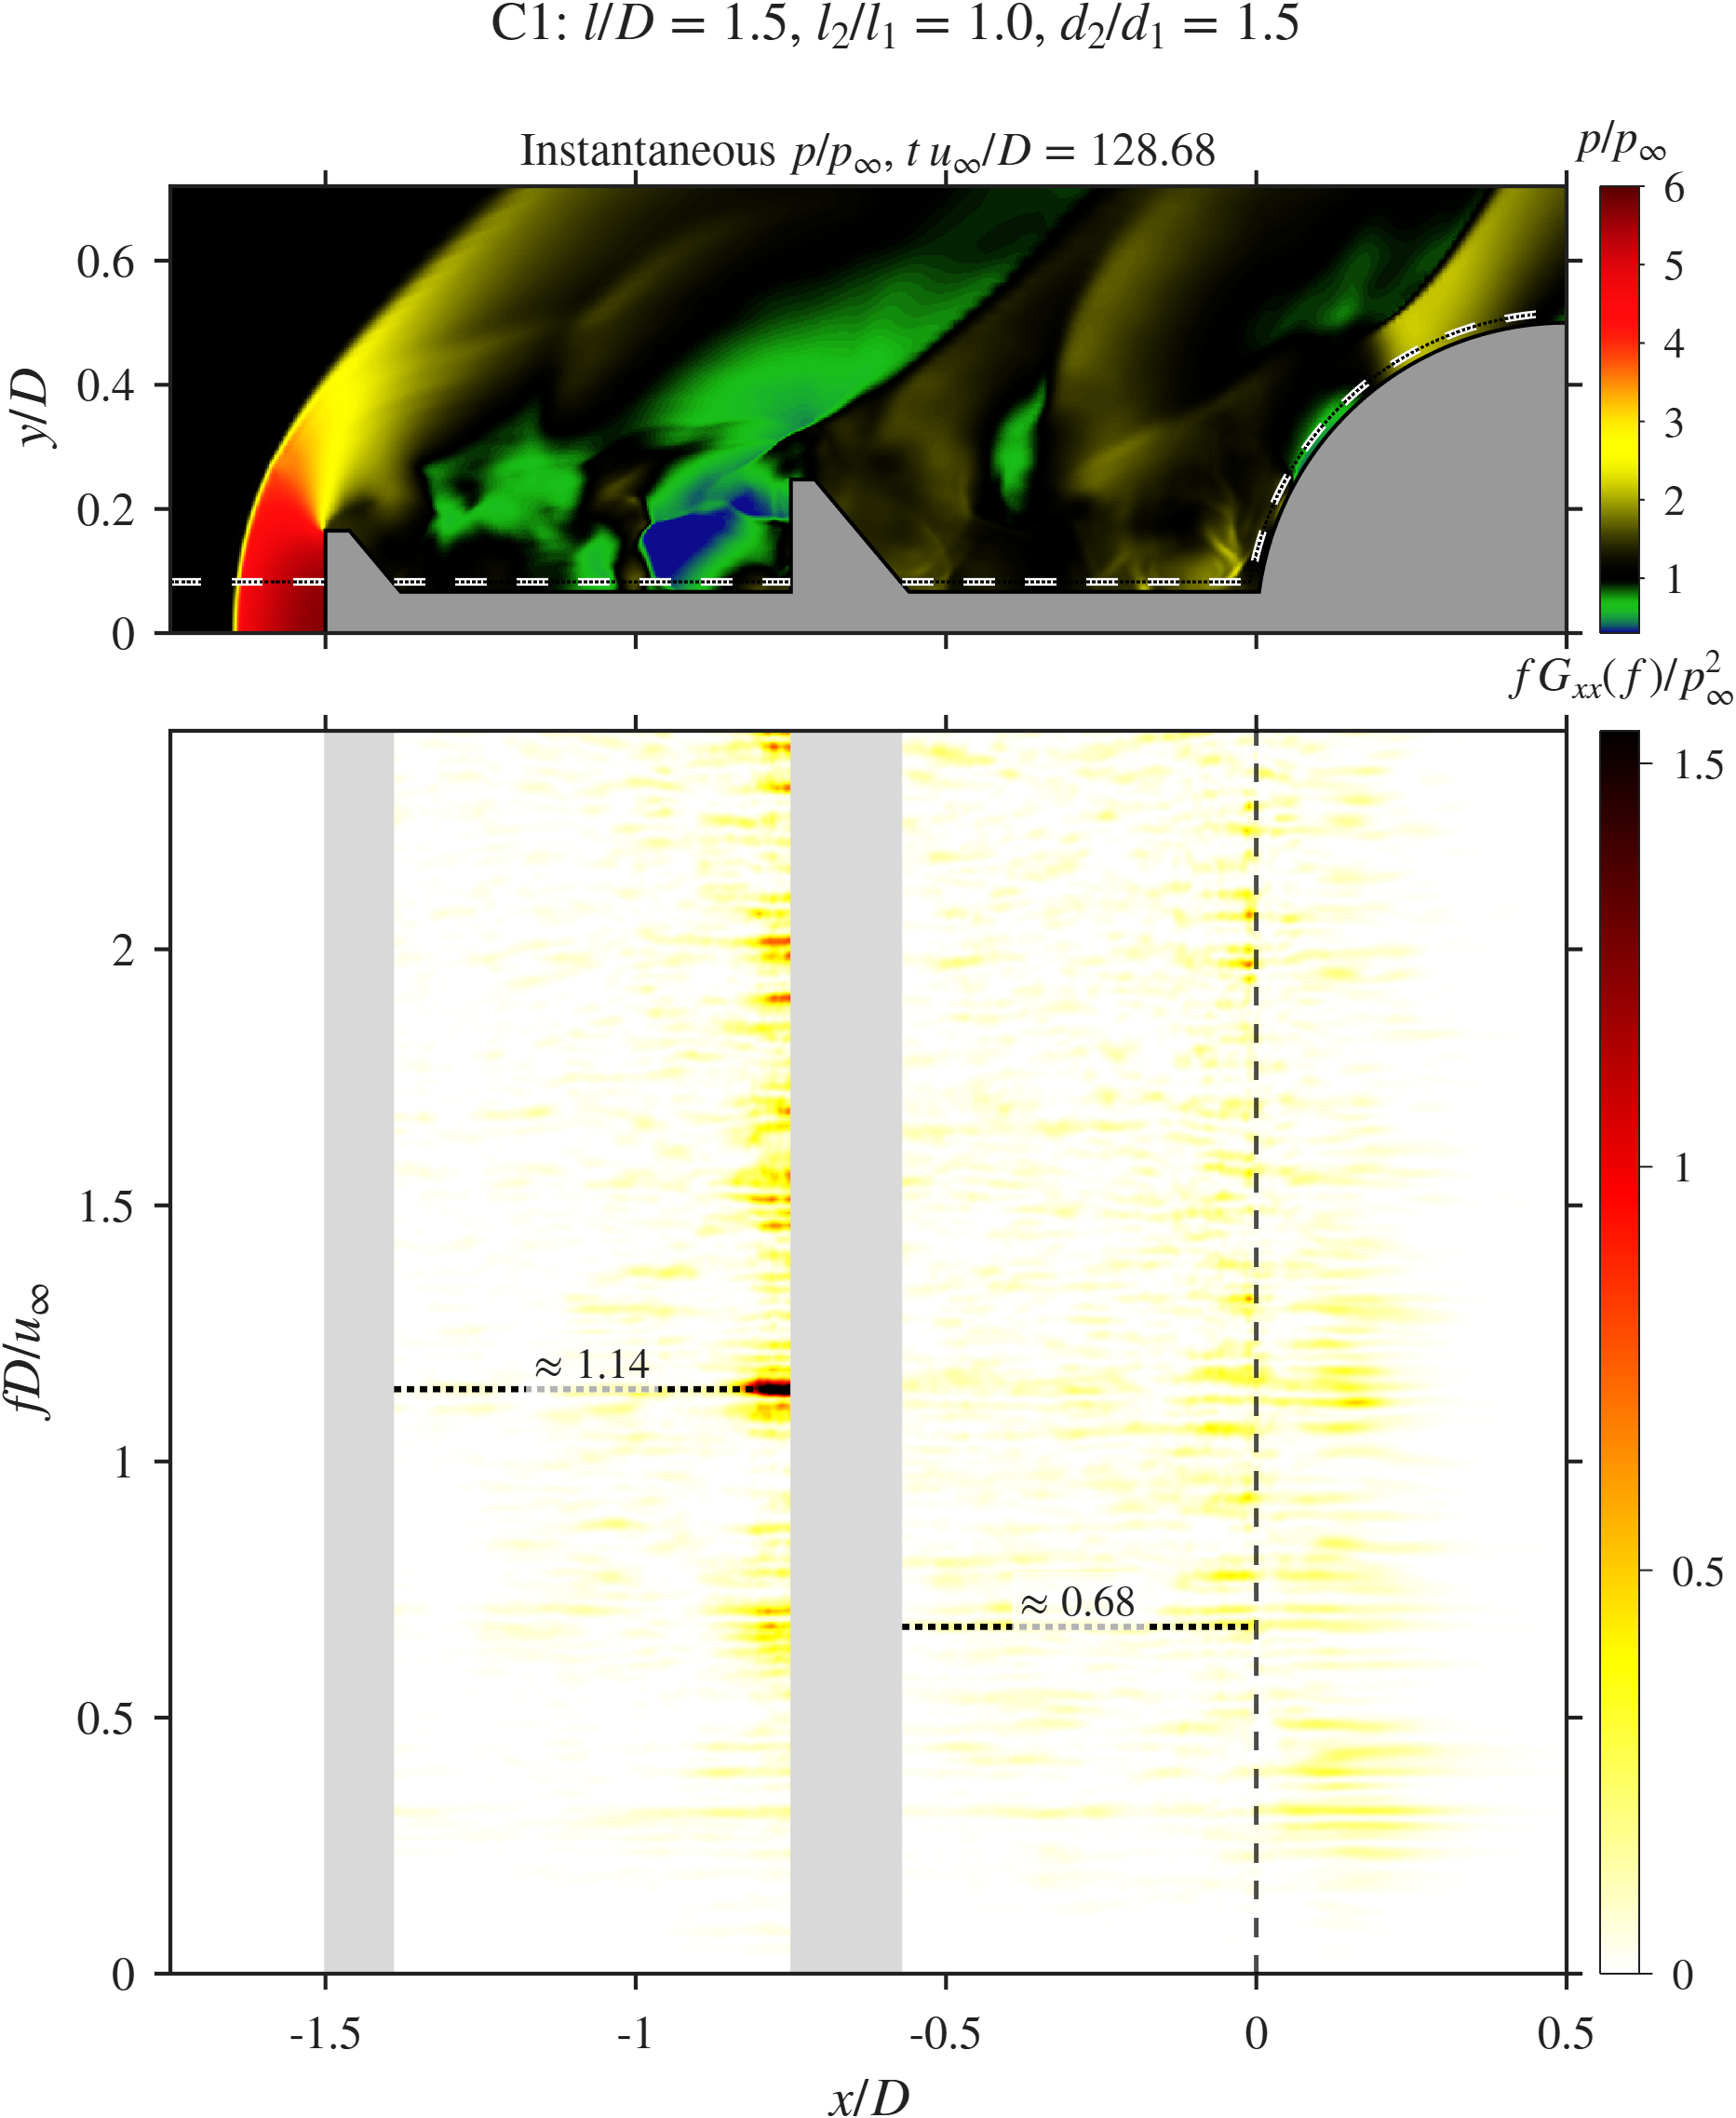
\includegraphics[width=\linewidth]{C1_xf.png}\caption{C1}\end{subfigure}
  \caption{$x$--$f$ diagrams (premultiplied PSD $fG_{xx}/\pinf^2$ along the probe line) for SA and C1. Grey bands mark the disks.}
  \label{fig:sac1_xf}
\end{figure}

\paragraph{Probe signals and spectra.} Figure~\ref{fig:sac1_sig} shows the probe pressure and drag signals and their spectra. The SA pressure is close to periodic, with $\pbar = 1.78$ and $\psd = 0.71$, and its spectrum has one sharp peak at $St = 0.76$ with $\Pi \approx 3.6$. The drag signal ($\Cdm = 0.36$, $\sCd = 0.10$) peaks at the same $St = 0.76$, so the shoulder pressure and the body drag follow the same feedback loop.

C1 has a similar mean ($\pbar = 1.86$, 4.5\% higher) and standard deviation ($\psd = 0.73$, 2.8\% higher), but its spectrum spreads over $St \approx 0.3$ to 2.5. The highest peak, at $St = 1.12$, reaches only $\Pi \approx 0.37$, about 90\% below the SA peak. The drag is slightly higher ($\Cdm = 0.39$, $\sCd = 0.12$) and peaks at $St = 1.14$. The pressure and drag peaks of C1 lie close together (1.12 and 1.14) and match the $St \approx 1.14$ band at the second-disk face in Fig.~\ref{fig:sac1_xf}(b). This suggests that the impingement of the Cavity 1 shear layer on the second disk now sets the dominant frequency.

\begin{figure}[htbp]
  \centering
  \begin{subfigure}{\textwidth}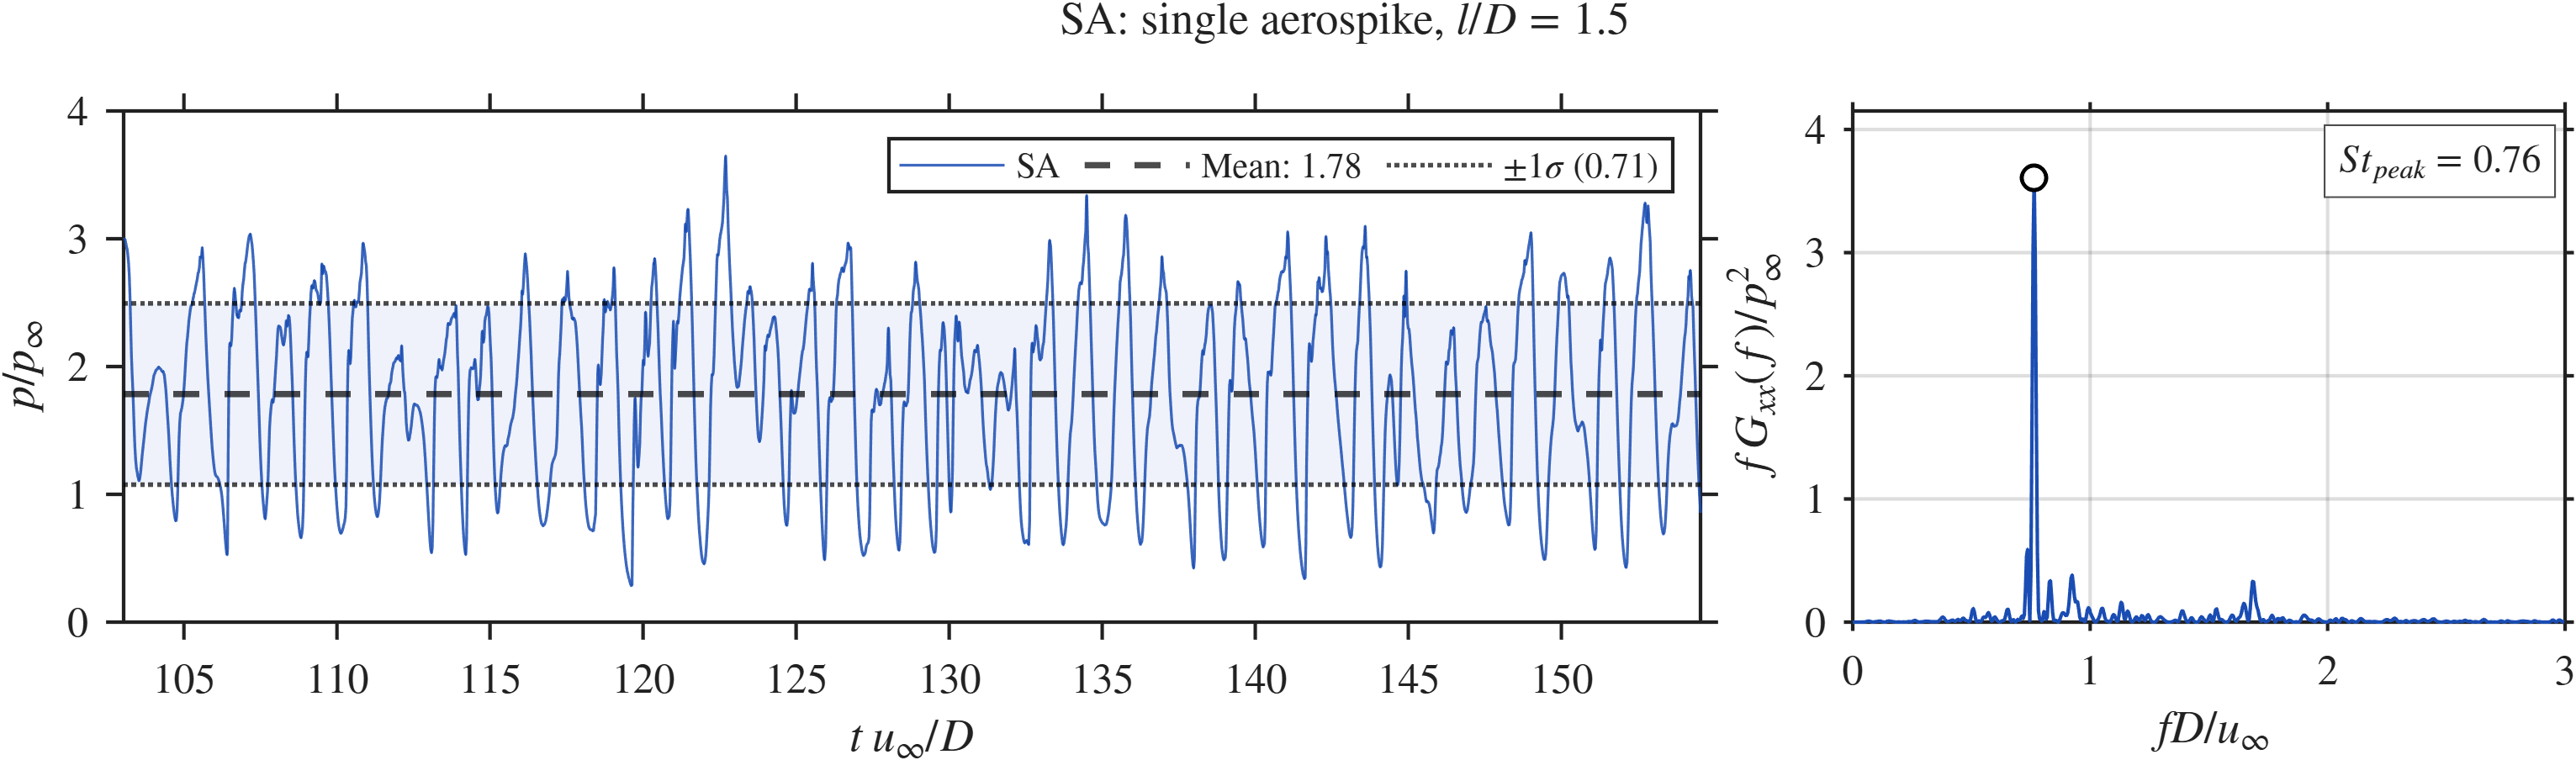
\includegraphics[width=\linewidth]{SA_psig.png}\caption{SA, pressure}\end{subfigure}\\
  \begin{subfigure}{\textwidth}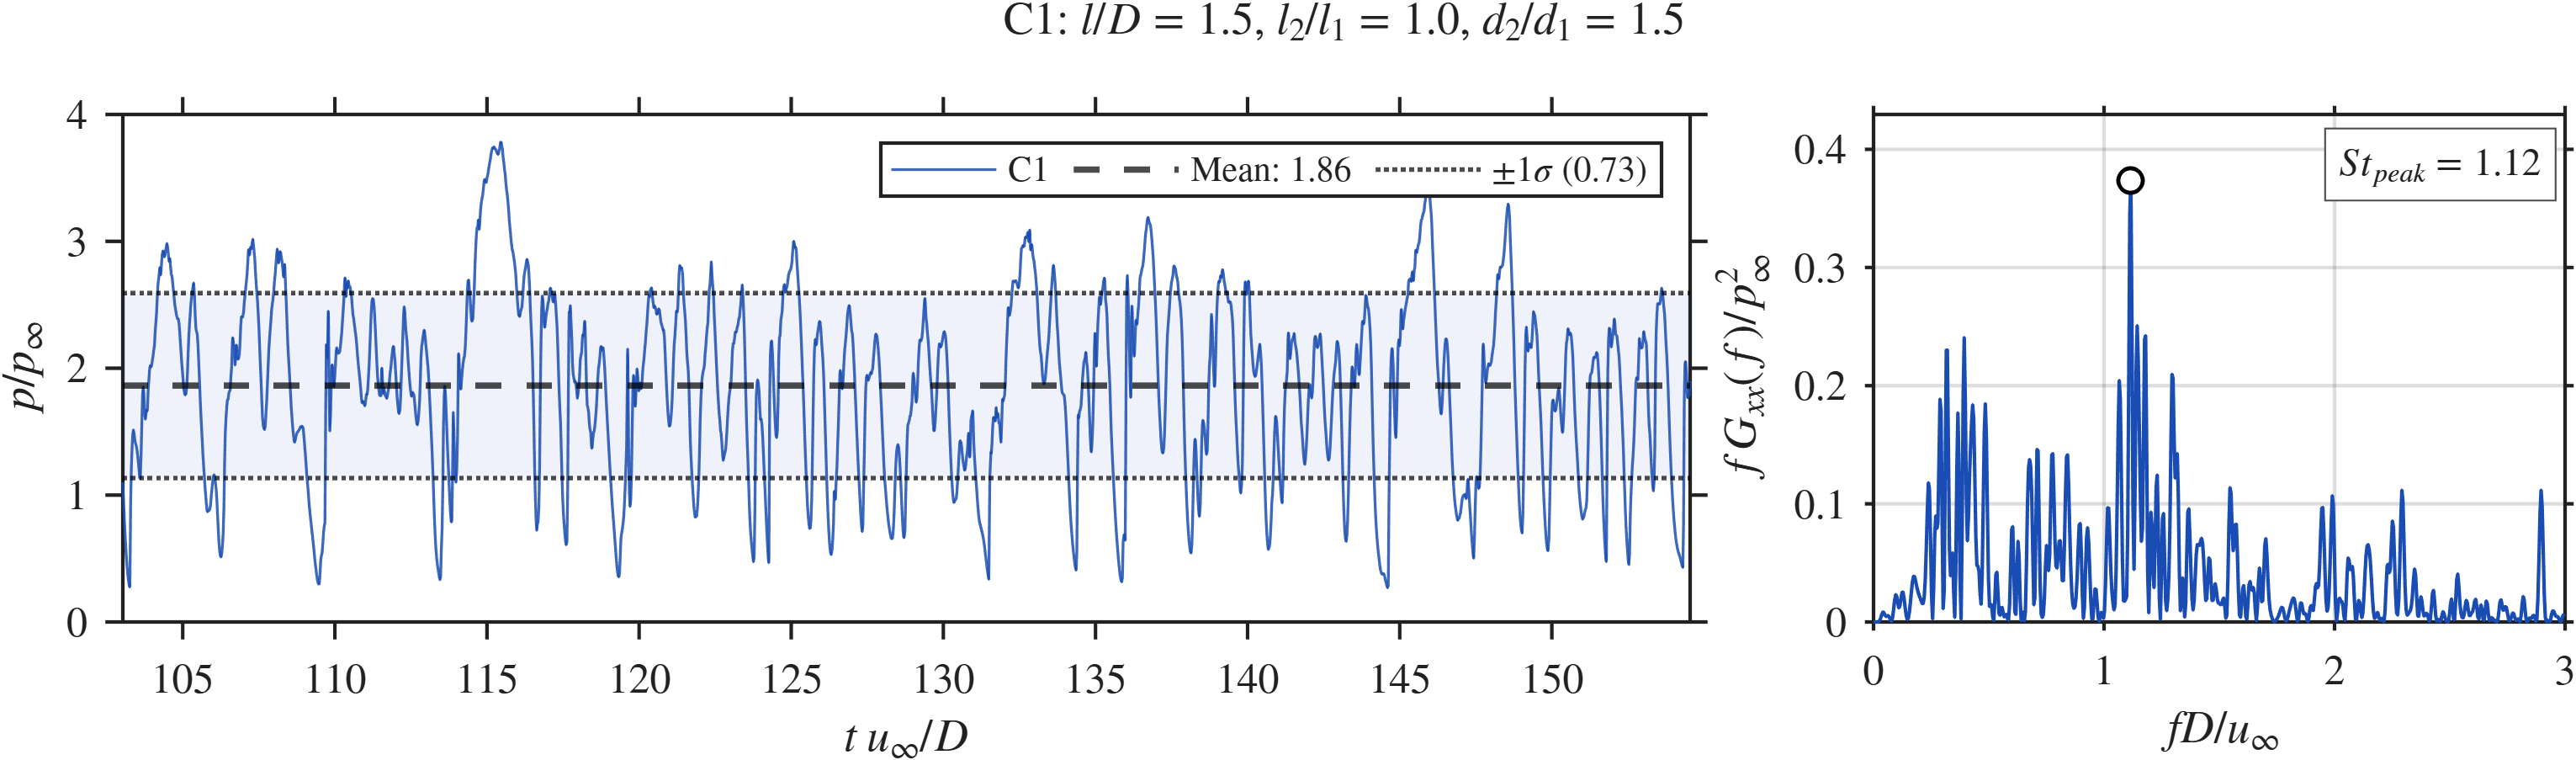
\includegraphics[width=\linewidth]{C1_psig.png}\caption{C1, pressure}\end{subfigure}\\
  \begin{subfigure}{\textwidth}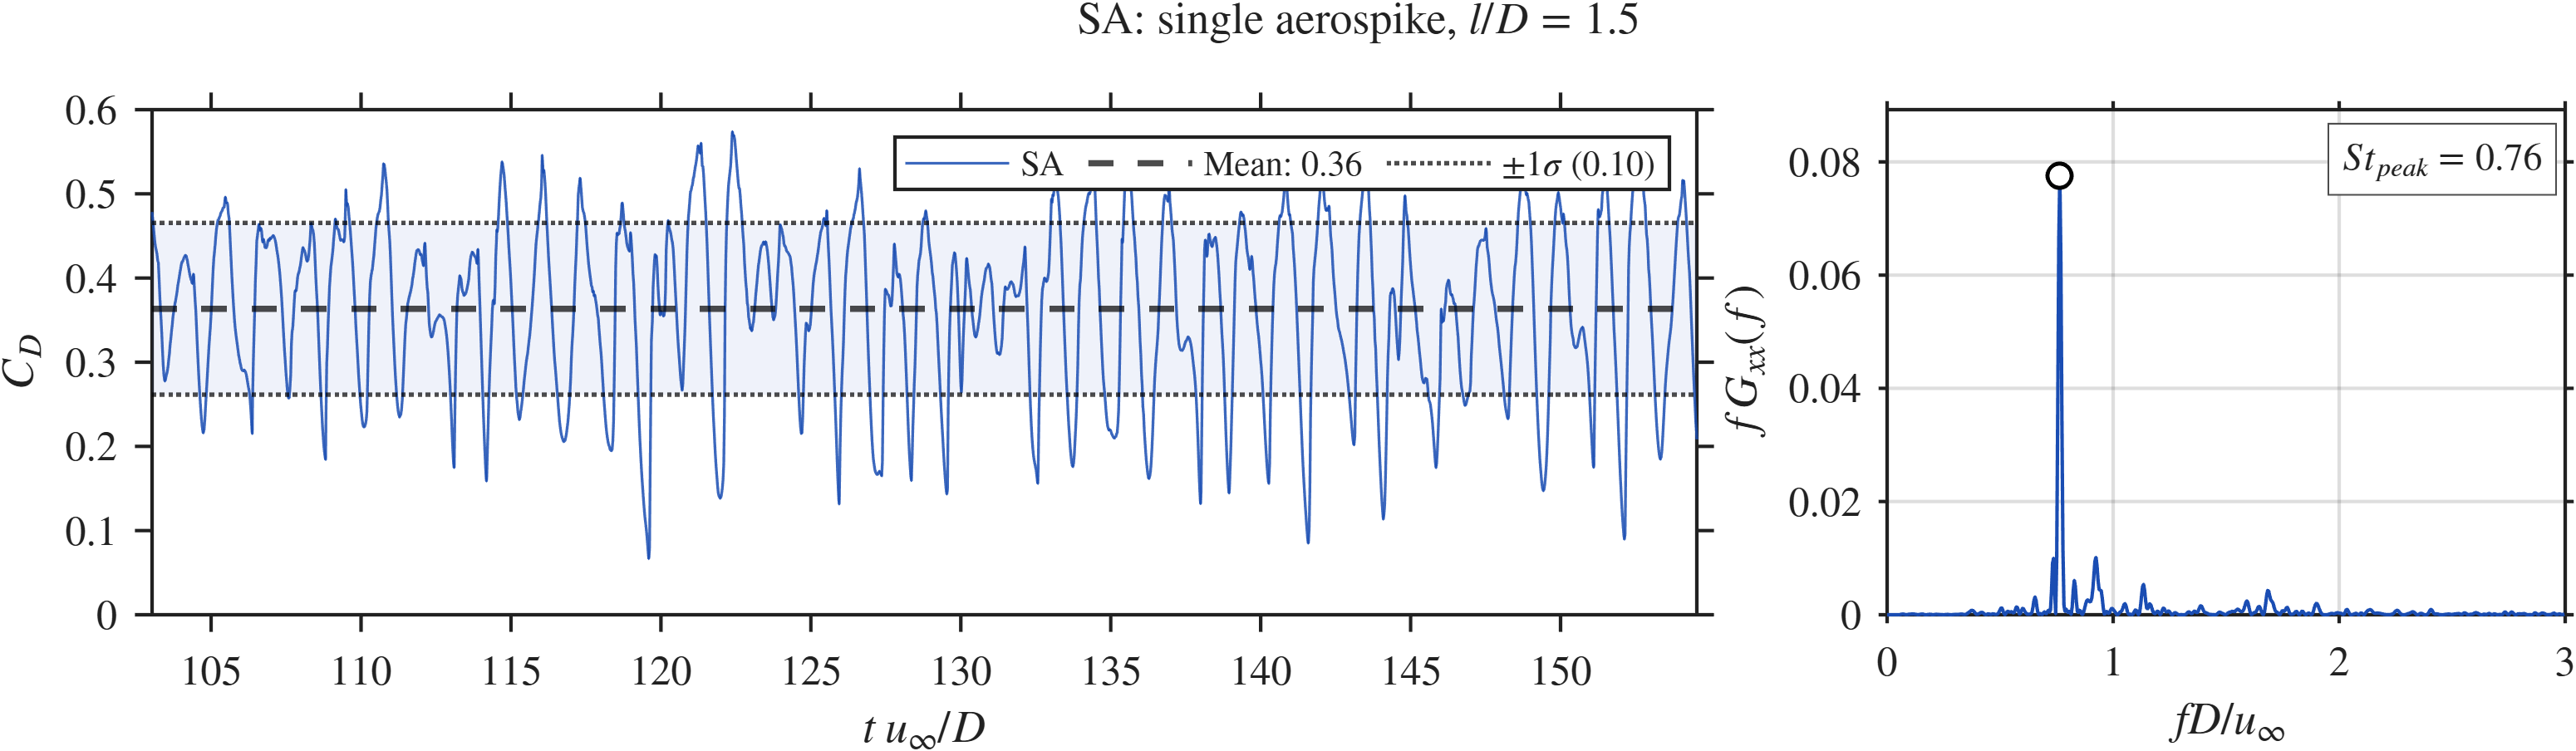
\includegraphics[width=\linewidth]{SA_dsig.png}\caption{SA, drag}\end{subfigure}\\
  \begin{subfigure}{\textwidth}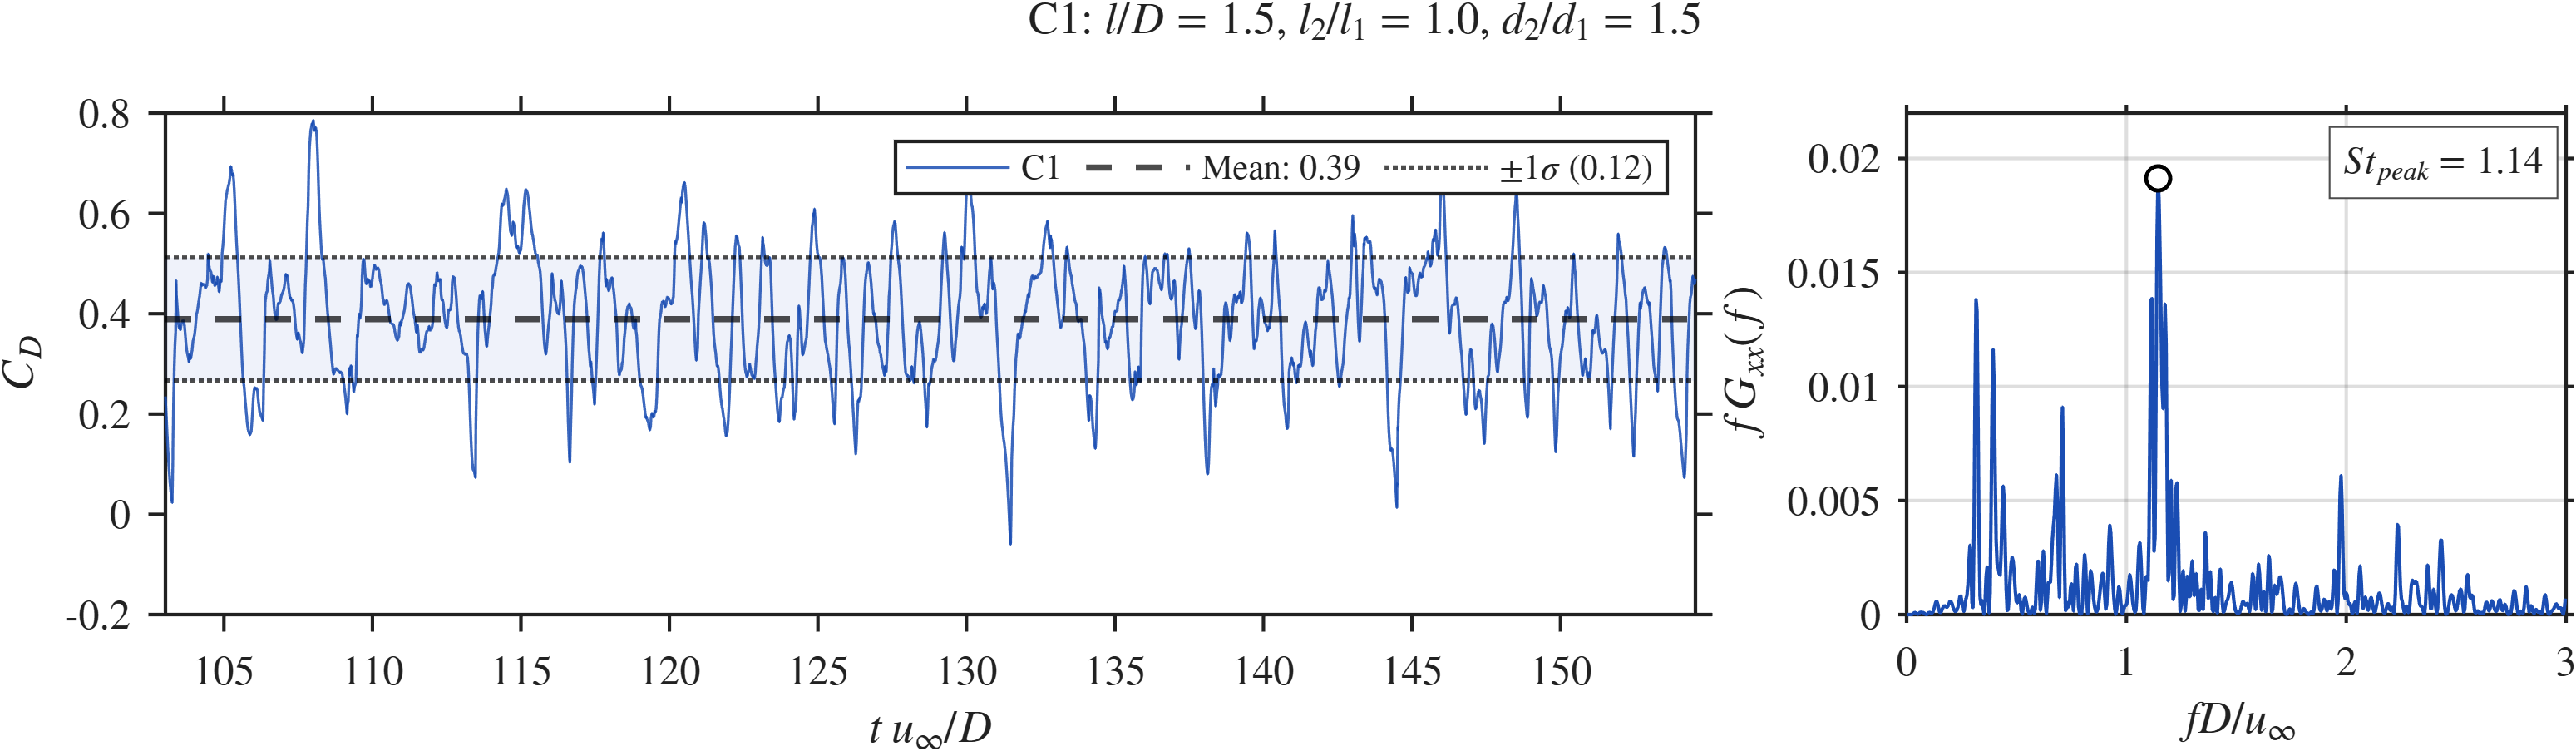
\includegraphics[width=\linewidth]{C1_dsig.png}\caption{C1, drag}\end{subfigure}
  \caption{Probe pressure $p/\pinf$ at $s/D \approx 0.4$ and drag coefficient $C_D$ over the sampling window (left) with their premultiplied spectra (right), for SA and C1.}
  \label{fig:sac1_sig}
\end{figure}

\paragraph{SPOD.} Figure~\ref{fig:sac1_spod} shows the SPOD spectra and the leading modes at the three highest peaks. The SA spectrum has one sharp peak at $St = 0.757$ ($\lambda_1 \approx 2.6\times10^{-5}$) with a wide gap to the second eigenvalue, which marks low-rank, tonal behaviour. Its mode is a set of large structures running from the disk along the shear layer to the shoulder. A smaller peak at $St = 0.912$ has finer structures in the downstream shear layer, and a peak at $St = 0.097$ is a slow breathing of the recirculation zone. In C1 the leading peak moves to $St = 0.291$ ($\lambda_1 \approx 1.3\times10^{-5}$), with a smaller gap to the second eigenvalue. The mode at $St = 0.291$ has large structures in both cavities with opposite sign across the second disk, which points to a coupled two-cavity oscillation. The second peak at $St = 0.718$, near the SA tone, is concentrated in Cavity 2 and at the shoulder. This suggests that the SA-type loop survives in Cavity 2 with less energy. The third peak at $St = 1.145$ is concentrated around the second disk and matches the disk-face band of the $x$--$f$ diagram.

\begin{figure}[htbp]
  \centering
  \begin{subfigure}{0.85\textwidth}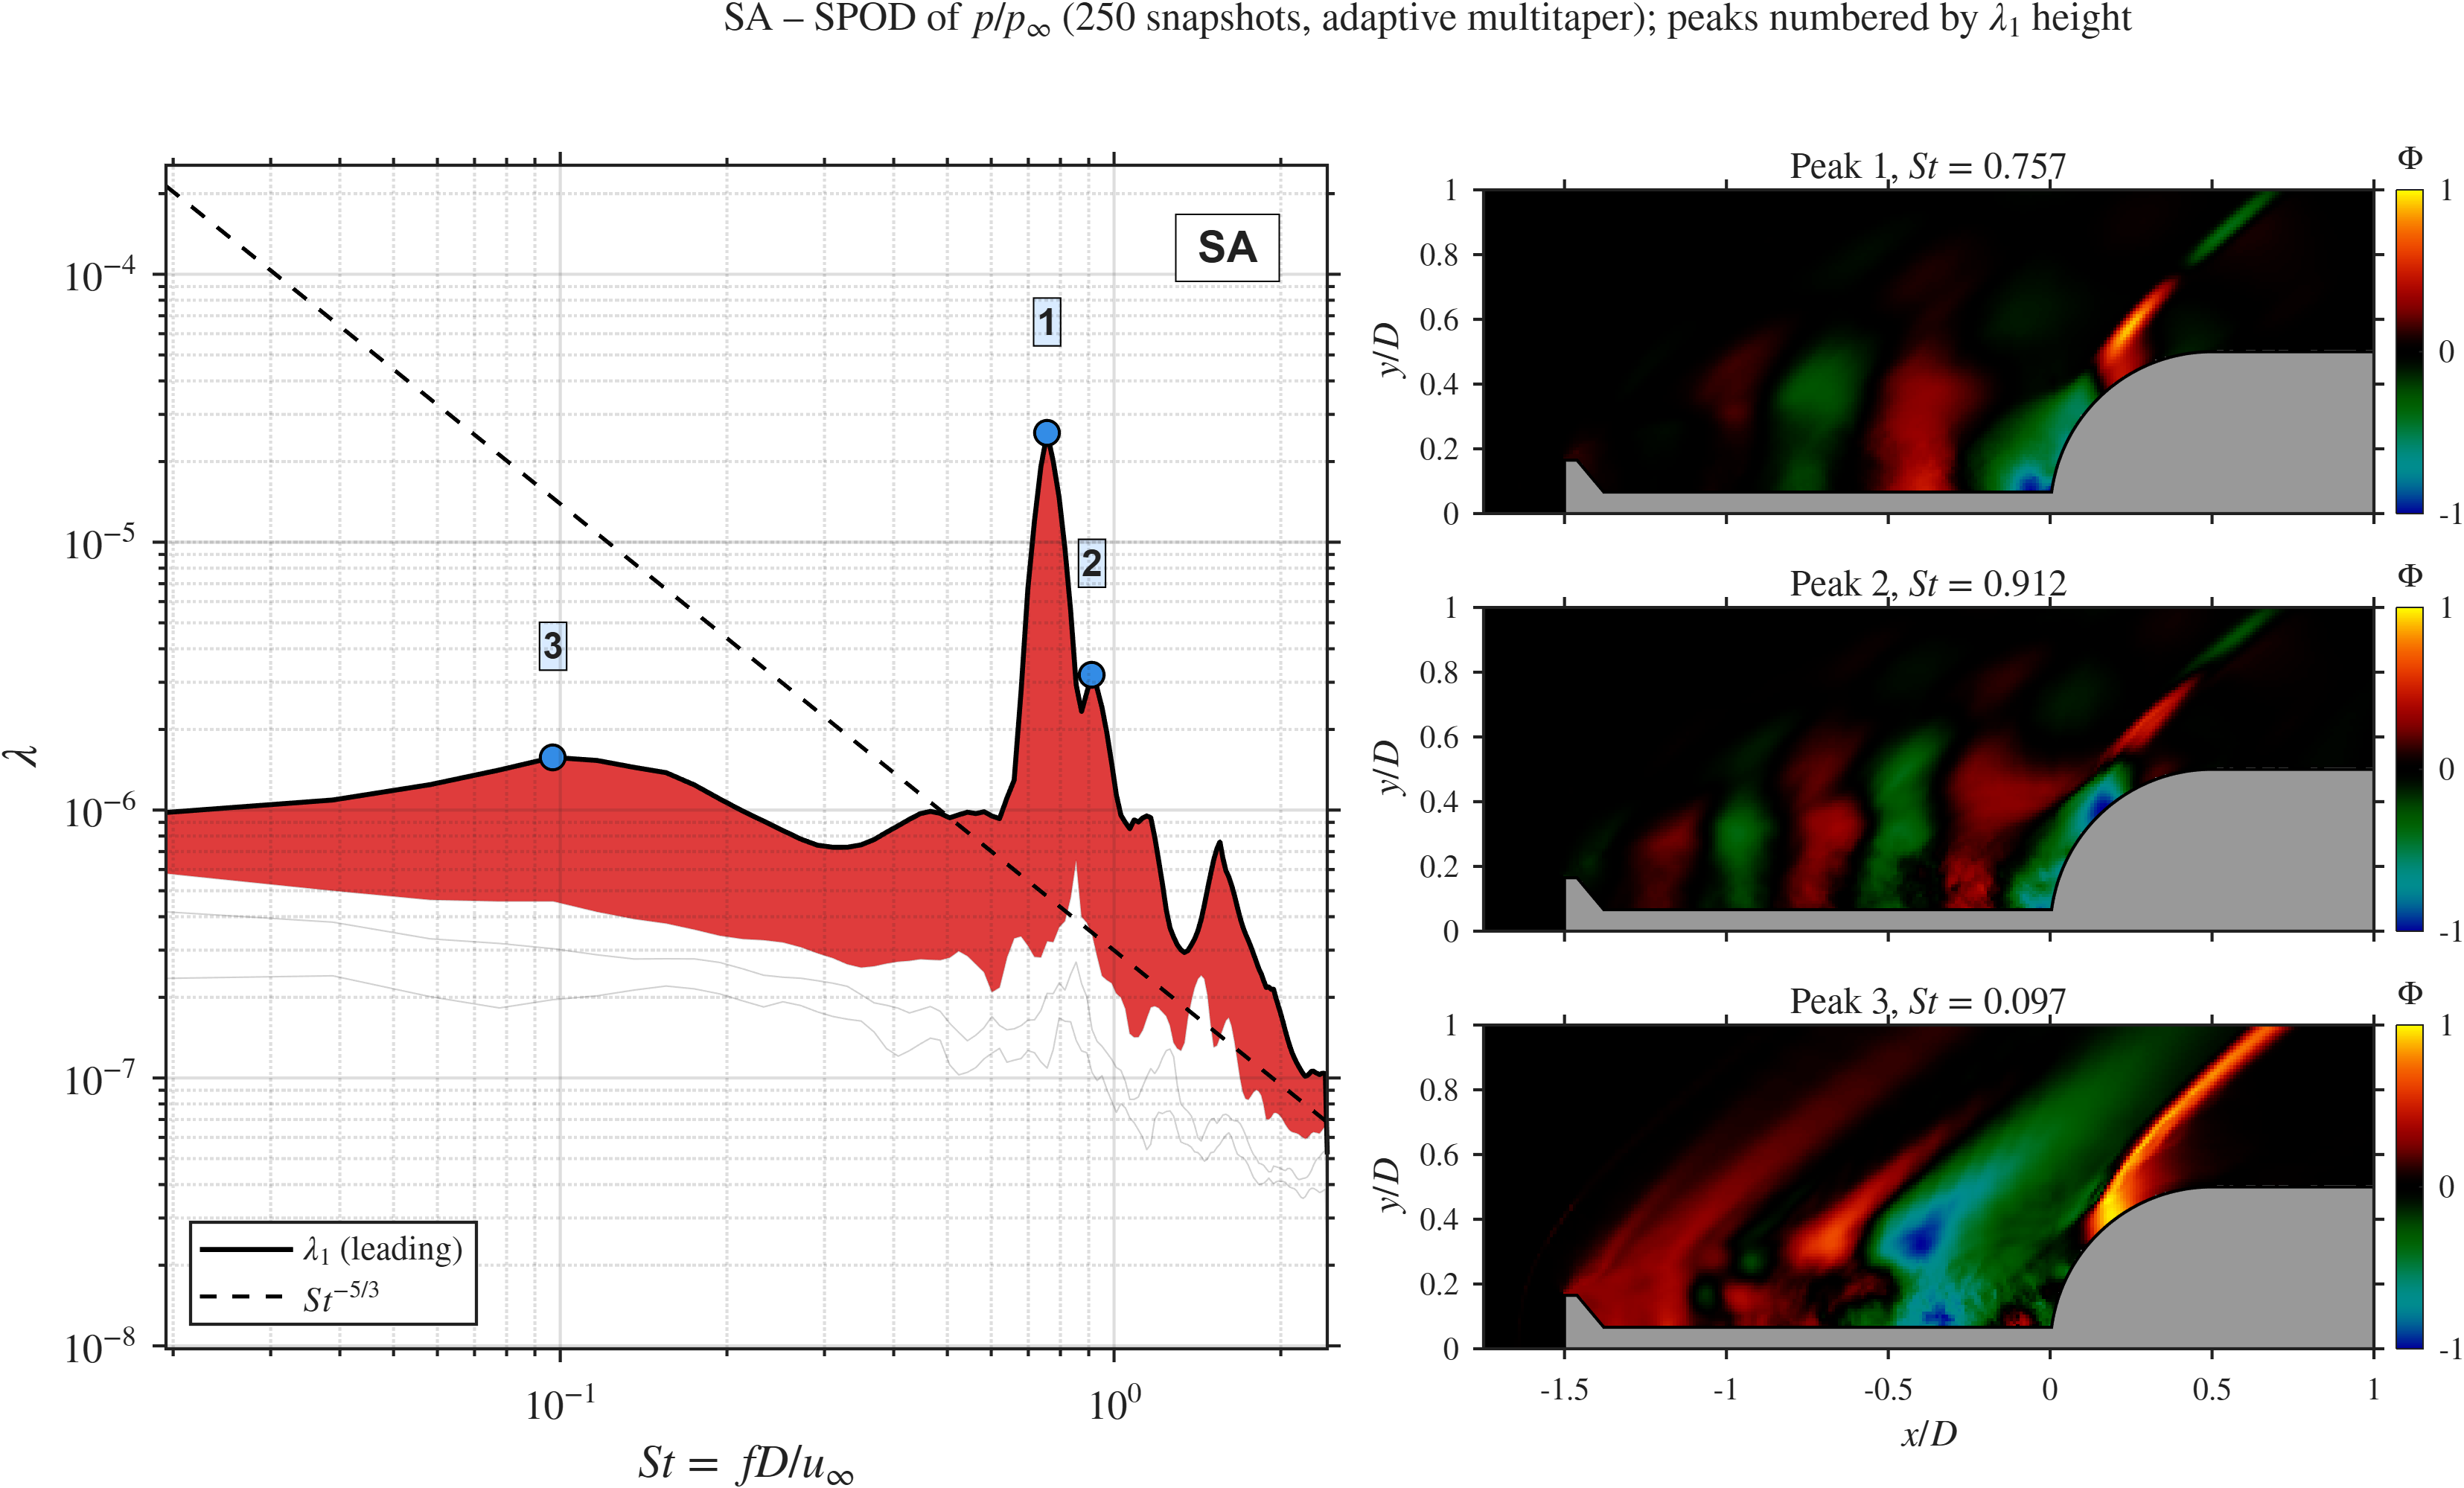
\includegraphics[width=\linewidth]{SA_spod.png}\caption{SA}\end{subfigure}\\
  \begin{subfigure}{0.85\textwidth}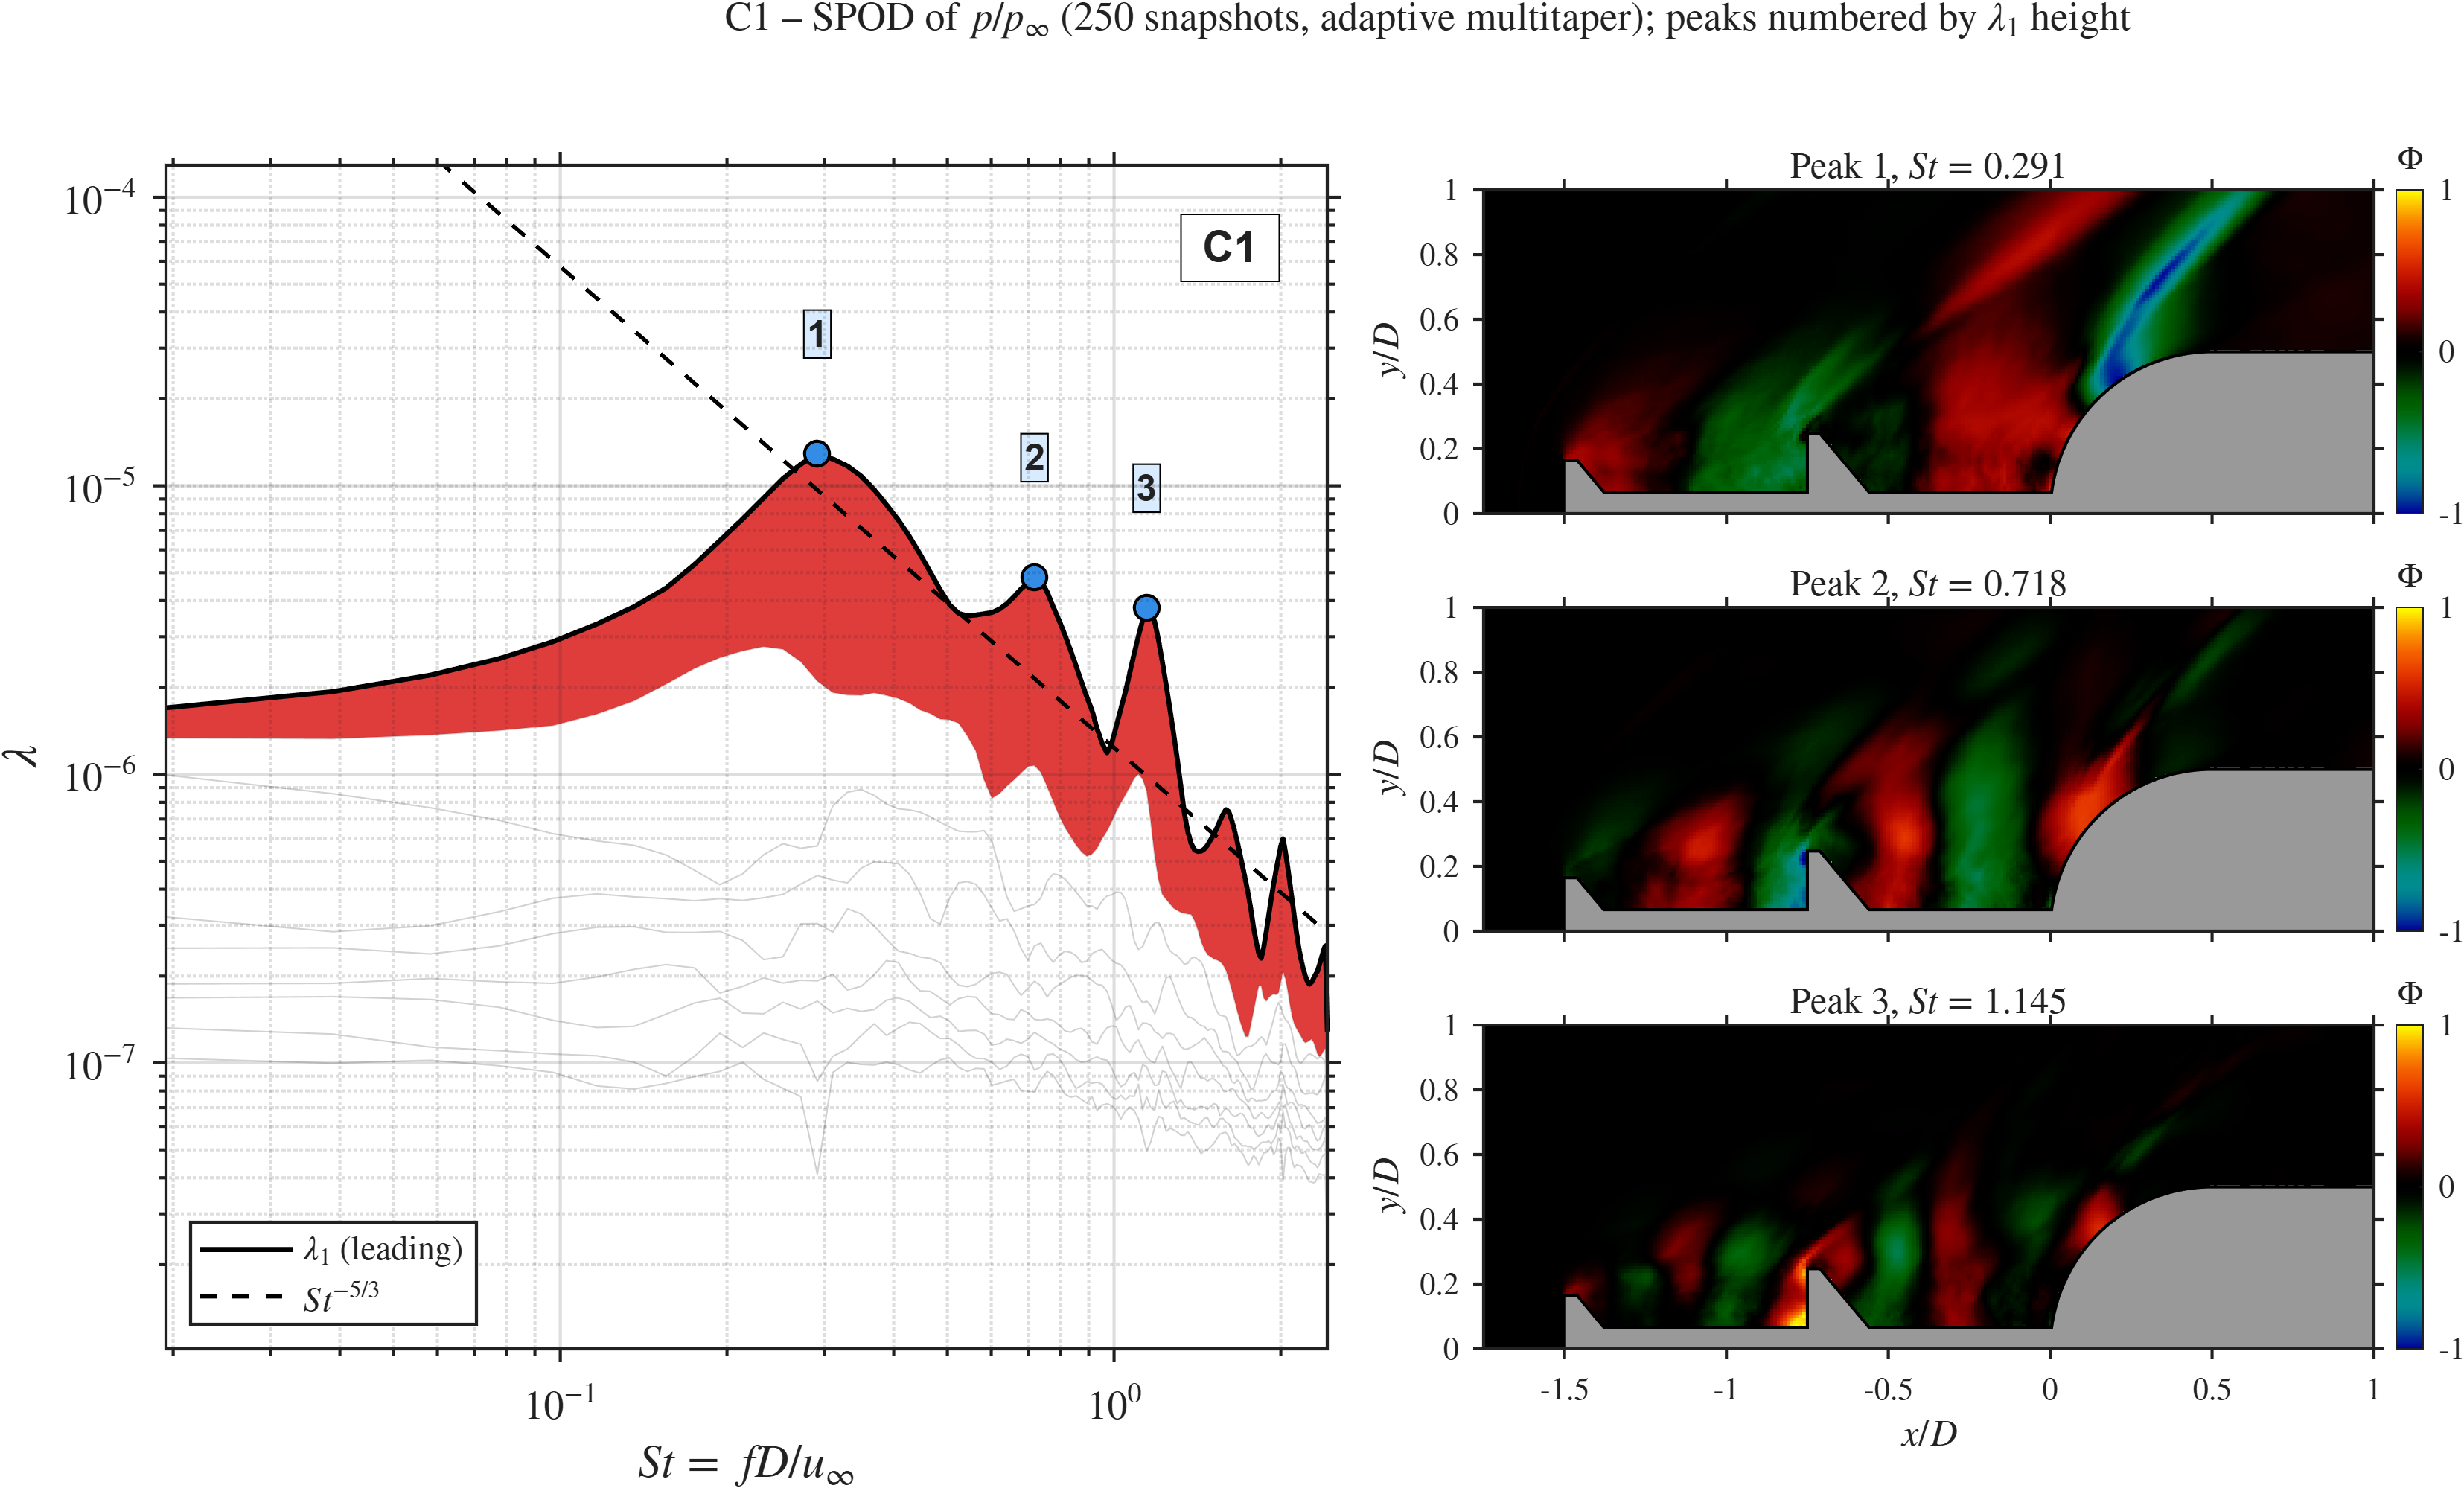
\includegraphics[width=\linewidth]{C1_spod.png}\caption{C1}\end{subfigure}
  \caption{SPOD of $p/\pinf$ (250 snapshots): leading eigenvalue $\lambda_1$ against $St$ (red band: gap to $\lambda_2$) and the real part of the leading mode at the three highest peaks.}
  \label{fig:sac1_spod}
\end{figure}

\paragraph{Summary.} Table~\ref{tab:sac1} lists the main numbers. The second disk does not reduce the mean loading or the overall fluctuation level at the shoulder. It changes the spectrum: the single SA tone at $St \approx 0.76$ is replaced by a broad band with a peak about ten times lower. The SPOD shows a new low-frequency coupled mode at $St \approx 0.29$ and a disk-face mode at $St \approx 1.1$, while the SA-type mode remains weaker in Cavity 2. This answers RQ1.

\begin{table}[htbp]
  \centering
  \caption{SA against the pivot DDAS C1. $\Delta$ is relative to SA.}
  \label{tab:sac1}
  \begin{tabular}{lccc}
    \toprule
    Metric & SA & C1 & $\Delta$ (\%) \\
    \midrule
    $\pbar$ & 1.78 & 1.86 & $+4.5$ \\
    $\psd$ & 0.71 & 0.73 & $+2.8$ \\
    $\Cdm$ & 0.36 & 0.39 & $+8.3$ \\
    $\sCd$ & 0.10 & 0.12 & $+20$ \\
    $St$ peak, pressure & 0.76 & 1.12 & -- \\
    $St$ peak, drag & 0.76 & 1.14 & -- \\
    Peak $\Pi$, pressure & $\approx 3.6$ & $\approx 0.37$ & $\approx -90$ \\
    SPOD leading $St$ & 0.757 & 0.291 & -- \\
    SPOD peak $\lambda_1$ & $\approx 2.6\times10^{-5}$ & $\approx 1.3\times10^{-5}$ & $\approx -50$ \\
    \bottomrule
  \end{tabular}
\end{table}

% ------------------------------------------------------------
\subsection{Effect of the gap ratio $\ltl$ (C3, C1, C2)}\label{sec:gap}

This sweep changes the axial position of the second disk at fixed $l/D = 1.5$ and $\dtd = 1.5$ (RQ3). In C3 ($\ltl = 0.5$) the disk sits at $x/D = -0.5$, which gives a long Cavity 1 ($l_1 = 1.0D$) and a short Cavity 2 ($l_2 = 0.5D$). In C2 ($\ltl = 2$) the disk sits at $x/D = -1.0$, which gives a short Cavity 1 ($l_1 = 0.5D$) and a long Cavity 2 ($l_2 = 1.0D$).

\paragraph{Mean flow and fluctuations.} Figure~\ref{fig:gap_ms} shows the mean and fluctuating pressure. In C3 the long Cavity 1 holds a large low-pressure region ($\pbar < 0.4$), and the short Cavity 2 is squeezed between the second disk and the hemisphere. The shoulder pressure is the highest of the sweep ($\pbar = 1.98$). In C2 the short Cavity 1 is barely visible, and the long Cavity 2 holds one large recirculation cell that looks like the SA cavity. Its shoulder pressure is the lowest of the sweep ($\pbar = 1.67$, 15.7\% below C3). C3 also has the strongest fluctuations. The face of the second disk and the short Cavity 2 reach $\psd > 0.8$, and the shoulder stays high, so the short cavity appears to trap and amplify the disturbances created where the Cavity 1 shear layer strikes the disk. In C2 the fluctuations concentrate at the shoulder and along the shear layer, with little activity in the short Cavity 1.

\begin{figure}[htbp]
  \centering
  \begin{subfigure}{0.49\textwidth}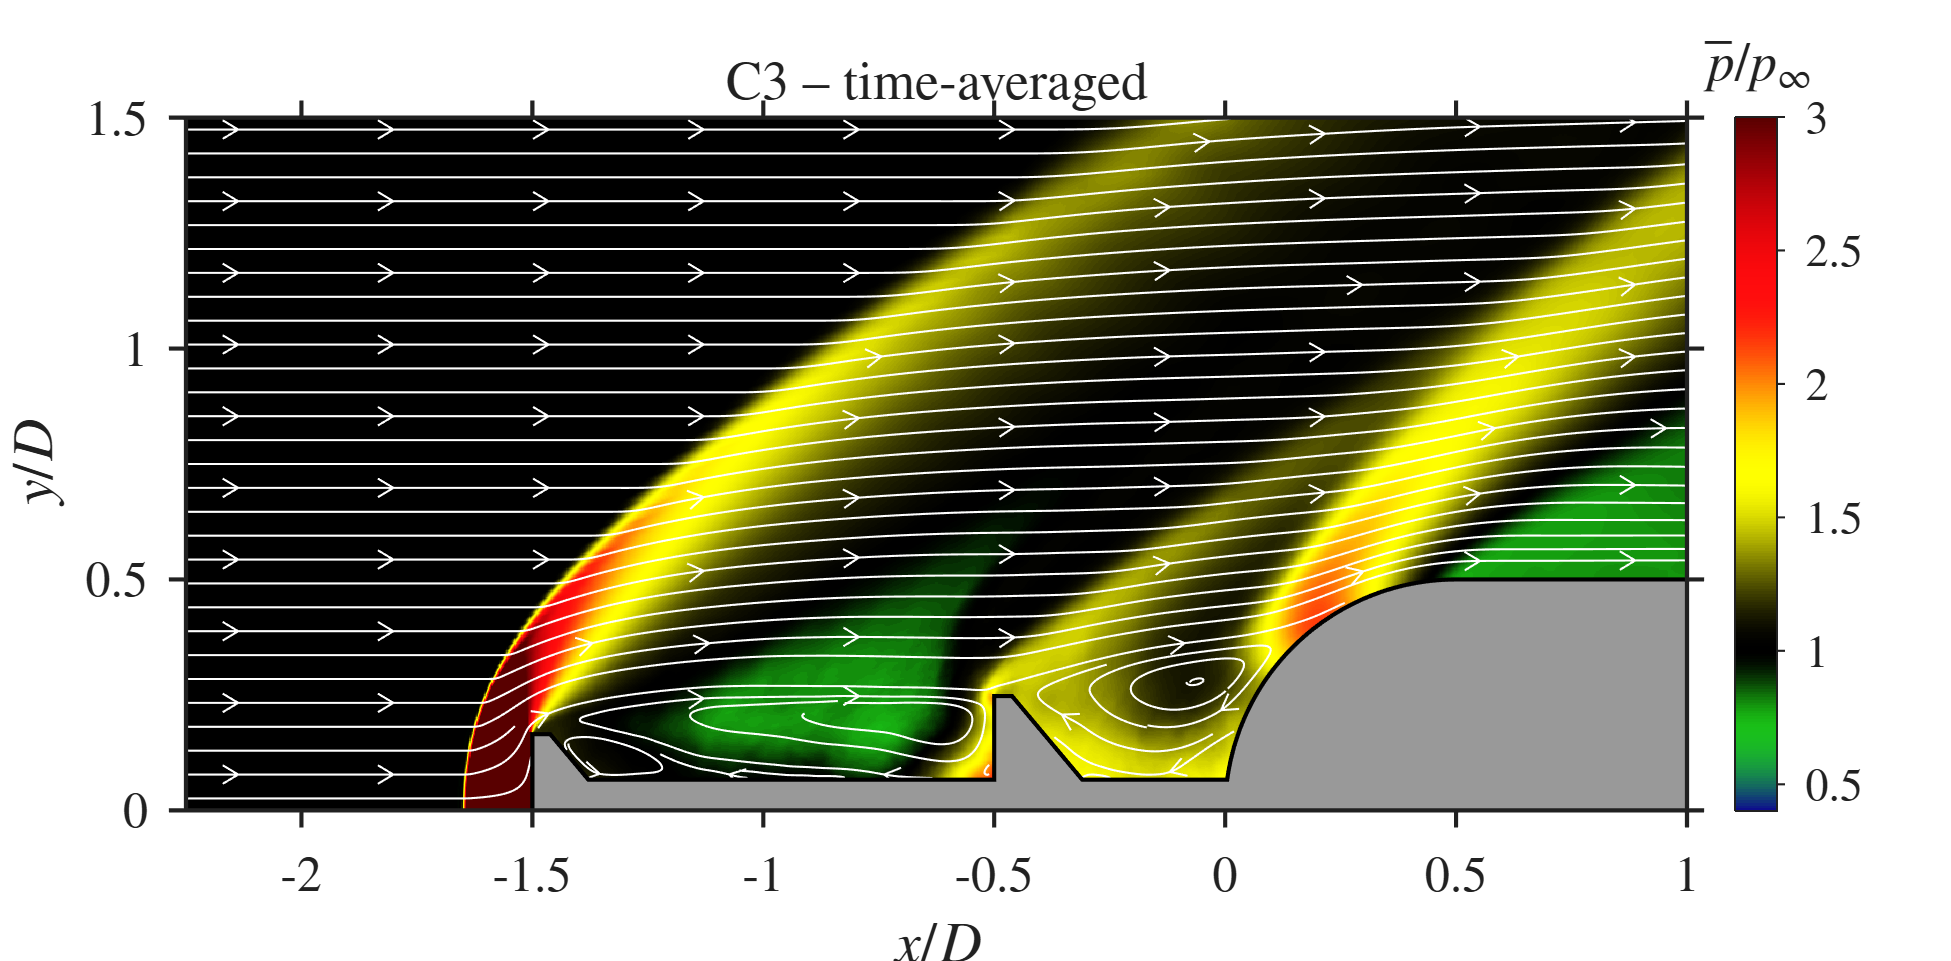
\includegraphics[width=\linewidth]{C3_mean.png}\caption{C3 ($\ltl = 0.5$), $\pbar$}\end{subfigure}
  \begin{subfigure}{0.49\textwidth}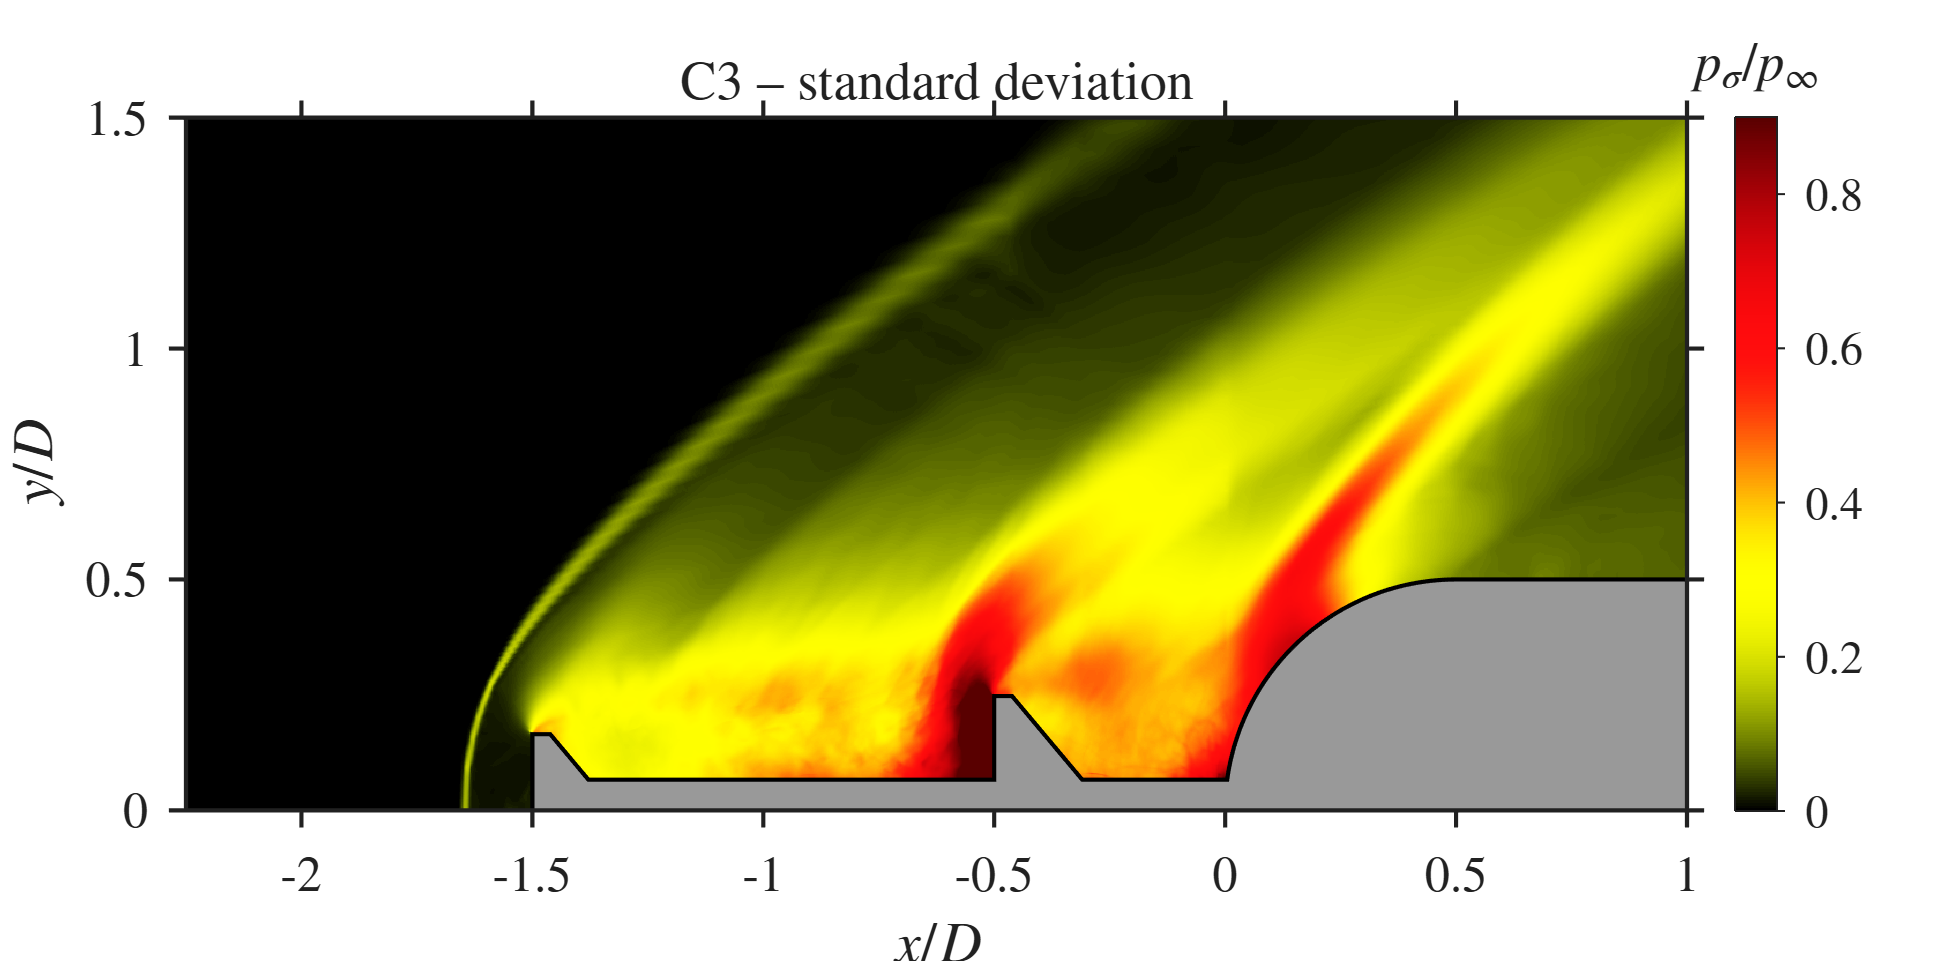
\includegraphics[width=\linewidth]{C3_std.png}\caption{C3, $\psd$}\end{subfigure}\\[2pt]
  \begin{subfigure}{0.49\textwidth}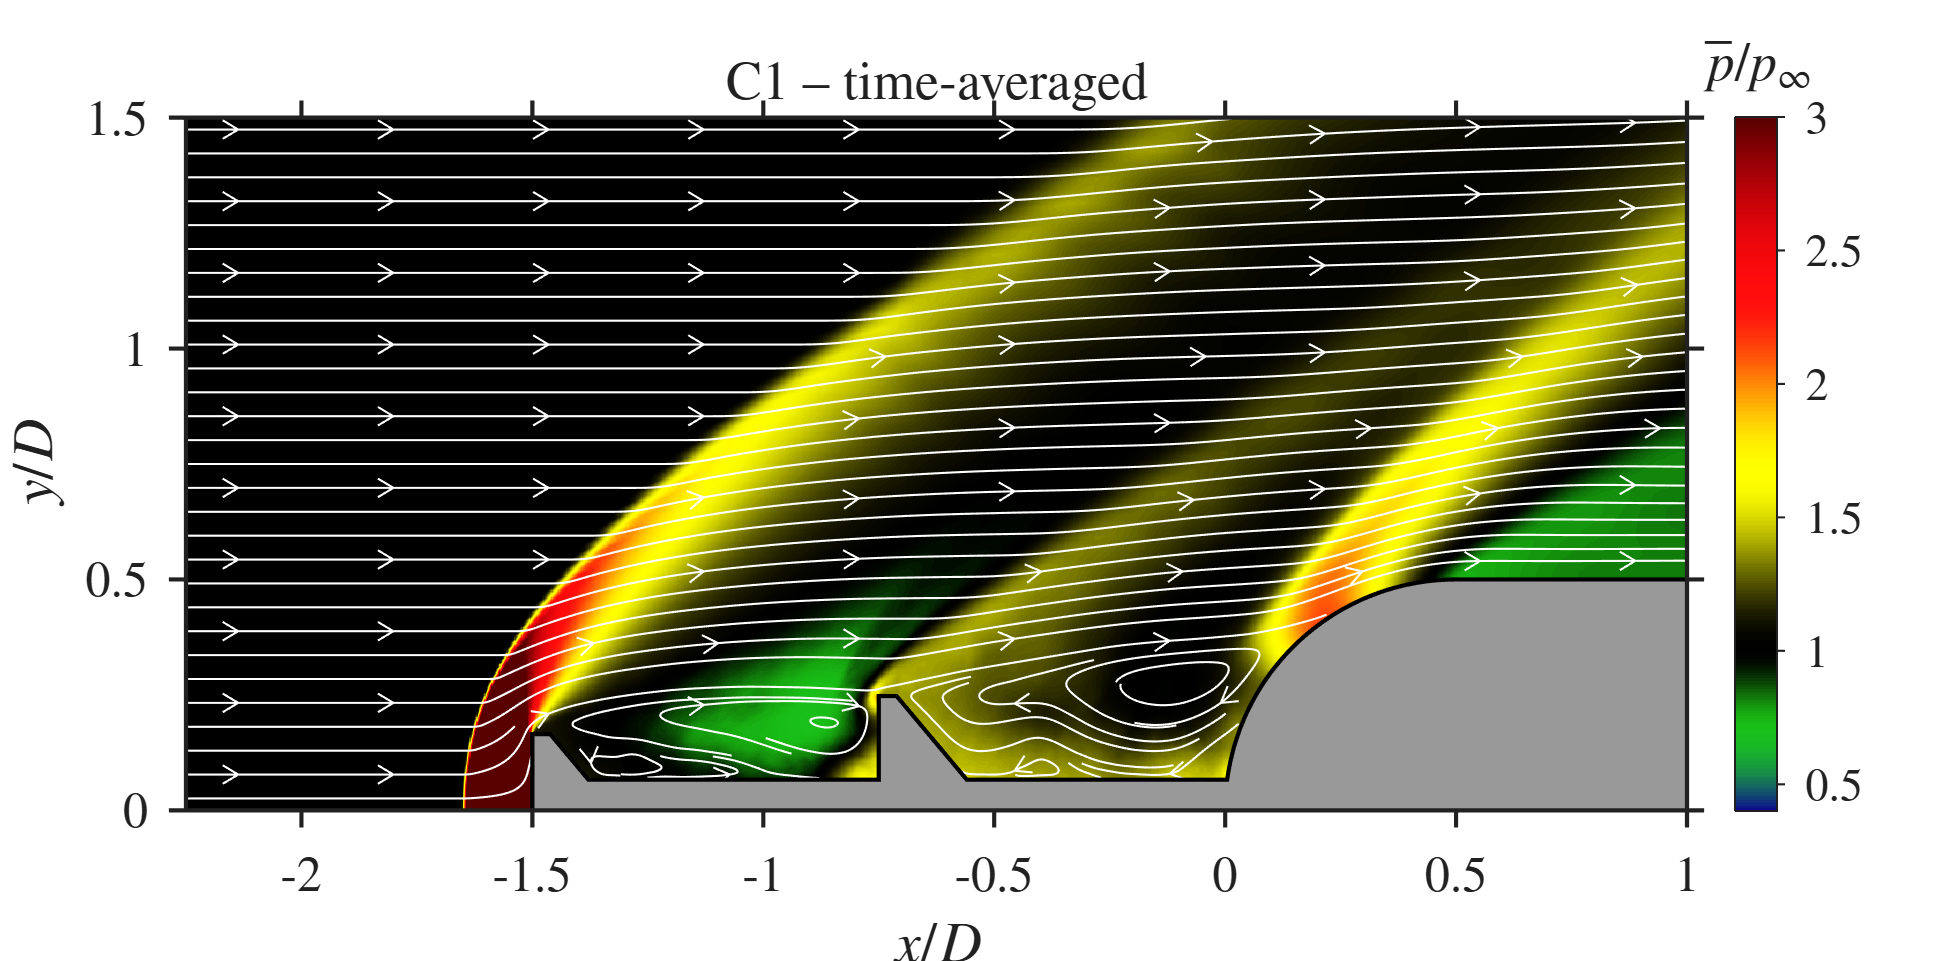
\includegraphics[width=\linewidth]{C1_mean.png}\caption{C1 ($\ltl = 1$), $\pbar$}\end{subfigure}
  \begin{subfigure}{0.49\textwidth}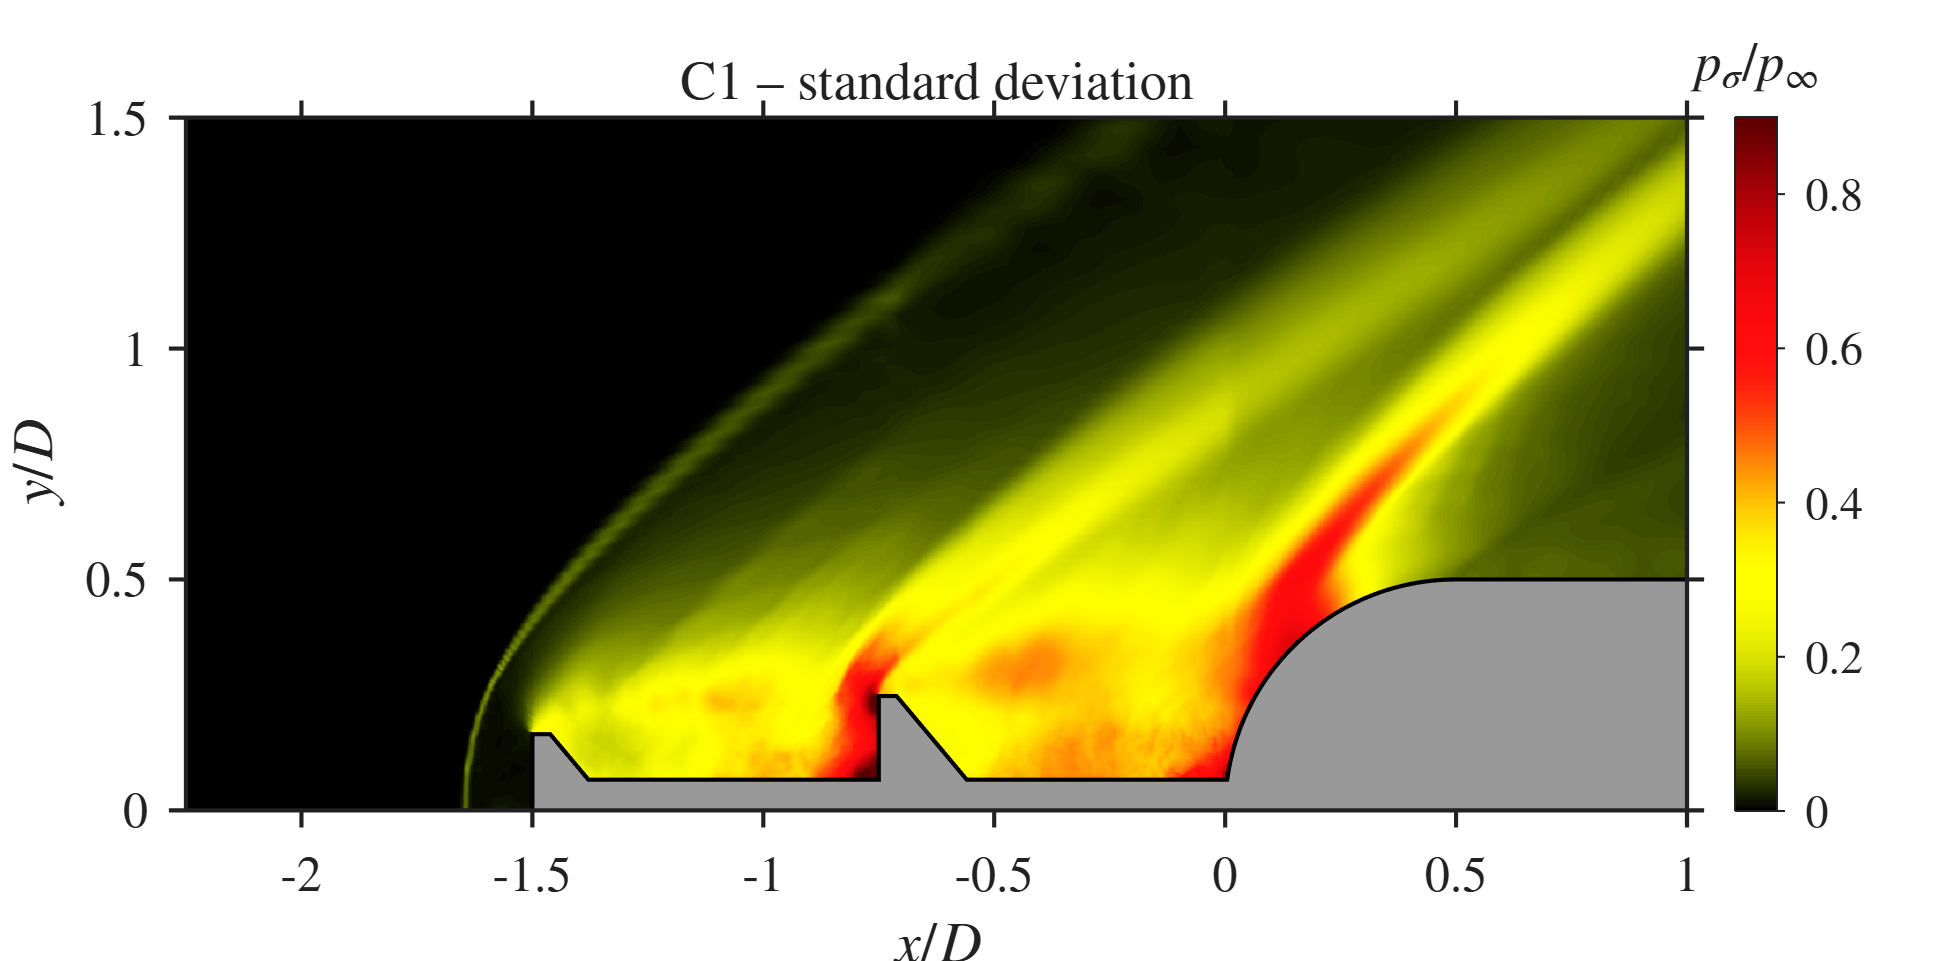
\includegraphics[width=\linewidth]{C1_std.png}\caption{C1, $\psd$}\end{subfigure}\\[2pt]
  \begin{subfigure}{0.49\textwidth}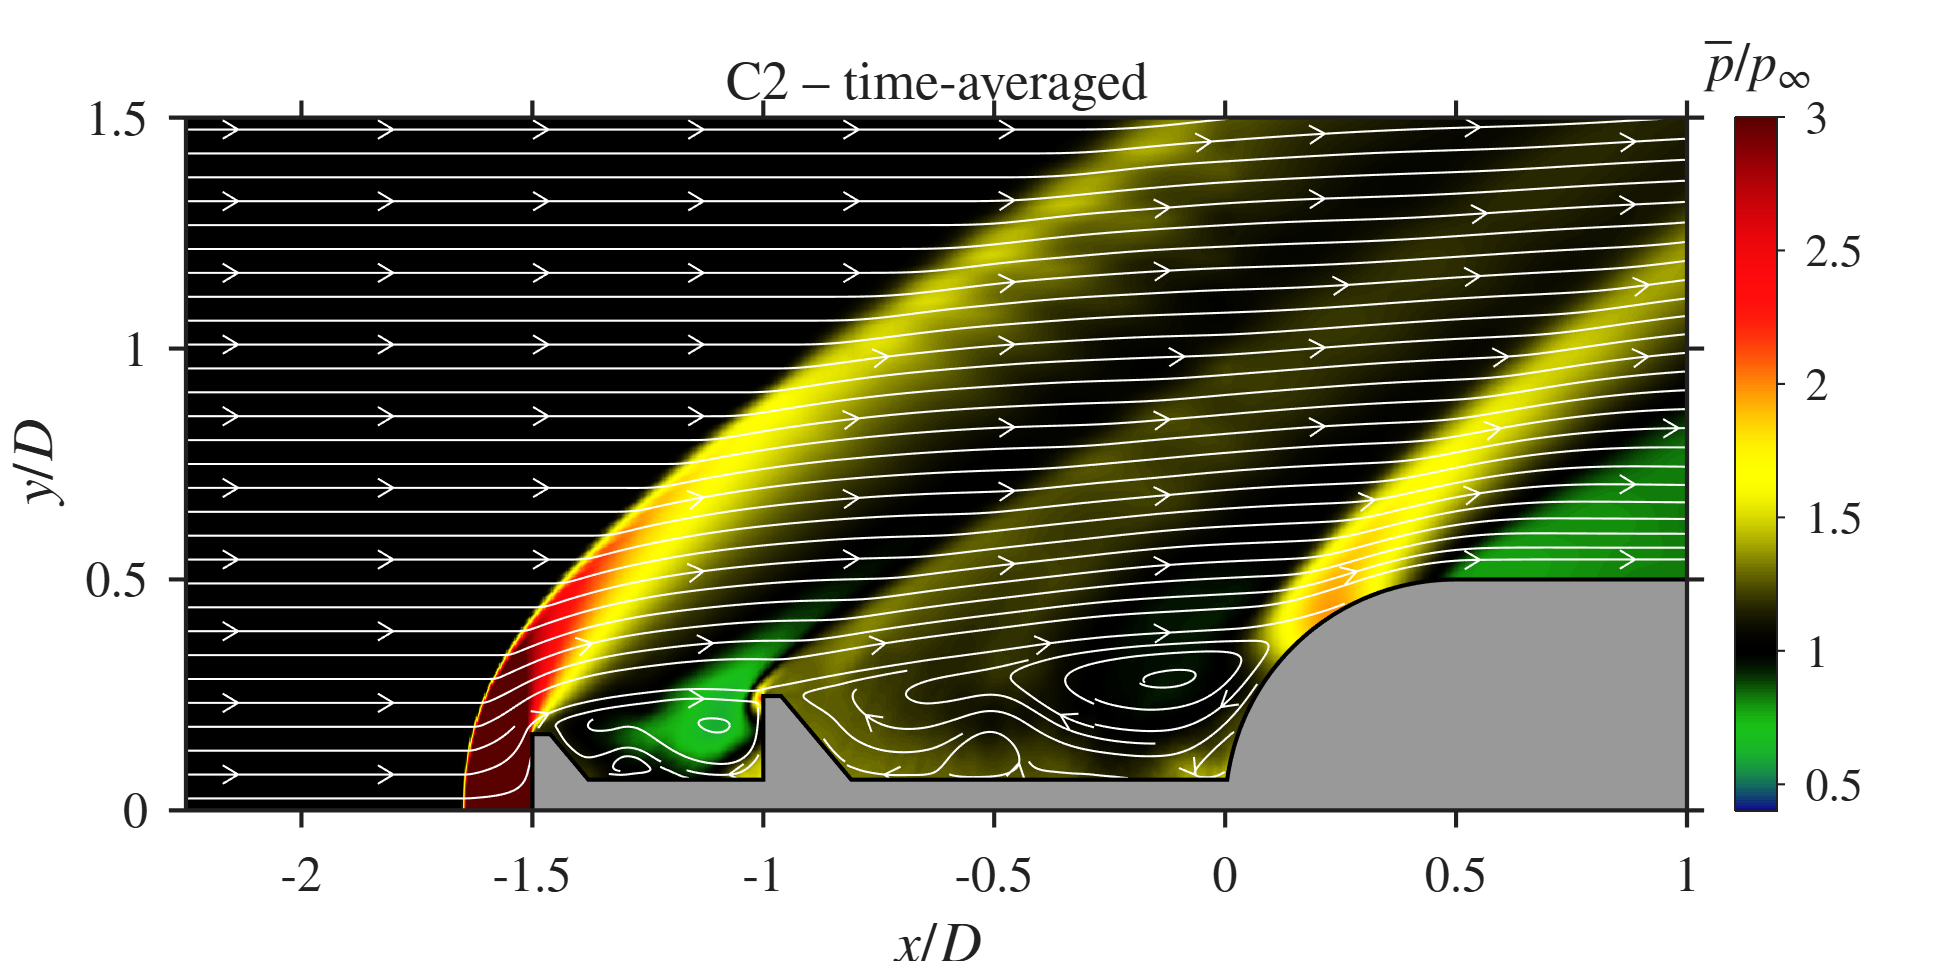
\includegraphics[width=\linewidth]{C2_mean.png}\caption{C2 ($\ltl = 2$), $\pbar$}\end{subfigure}
  \begin{subfigure}{0.49\textwidth}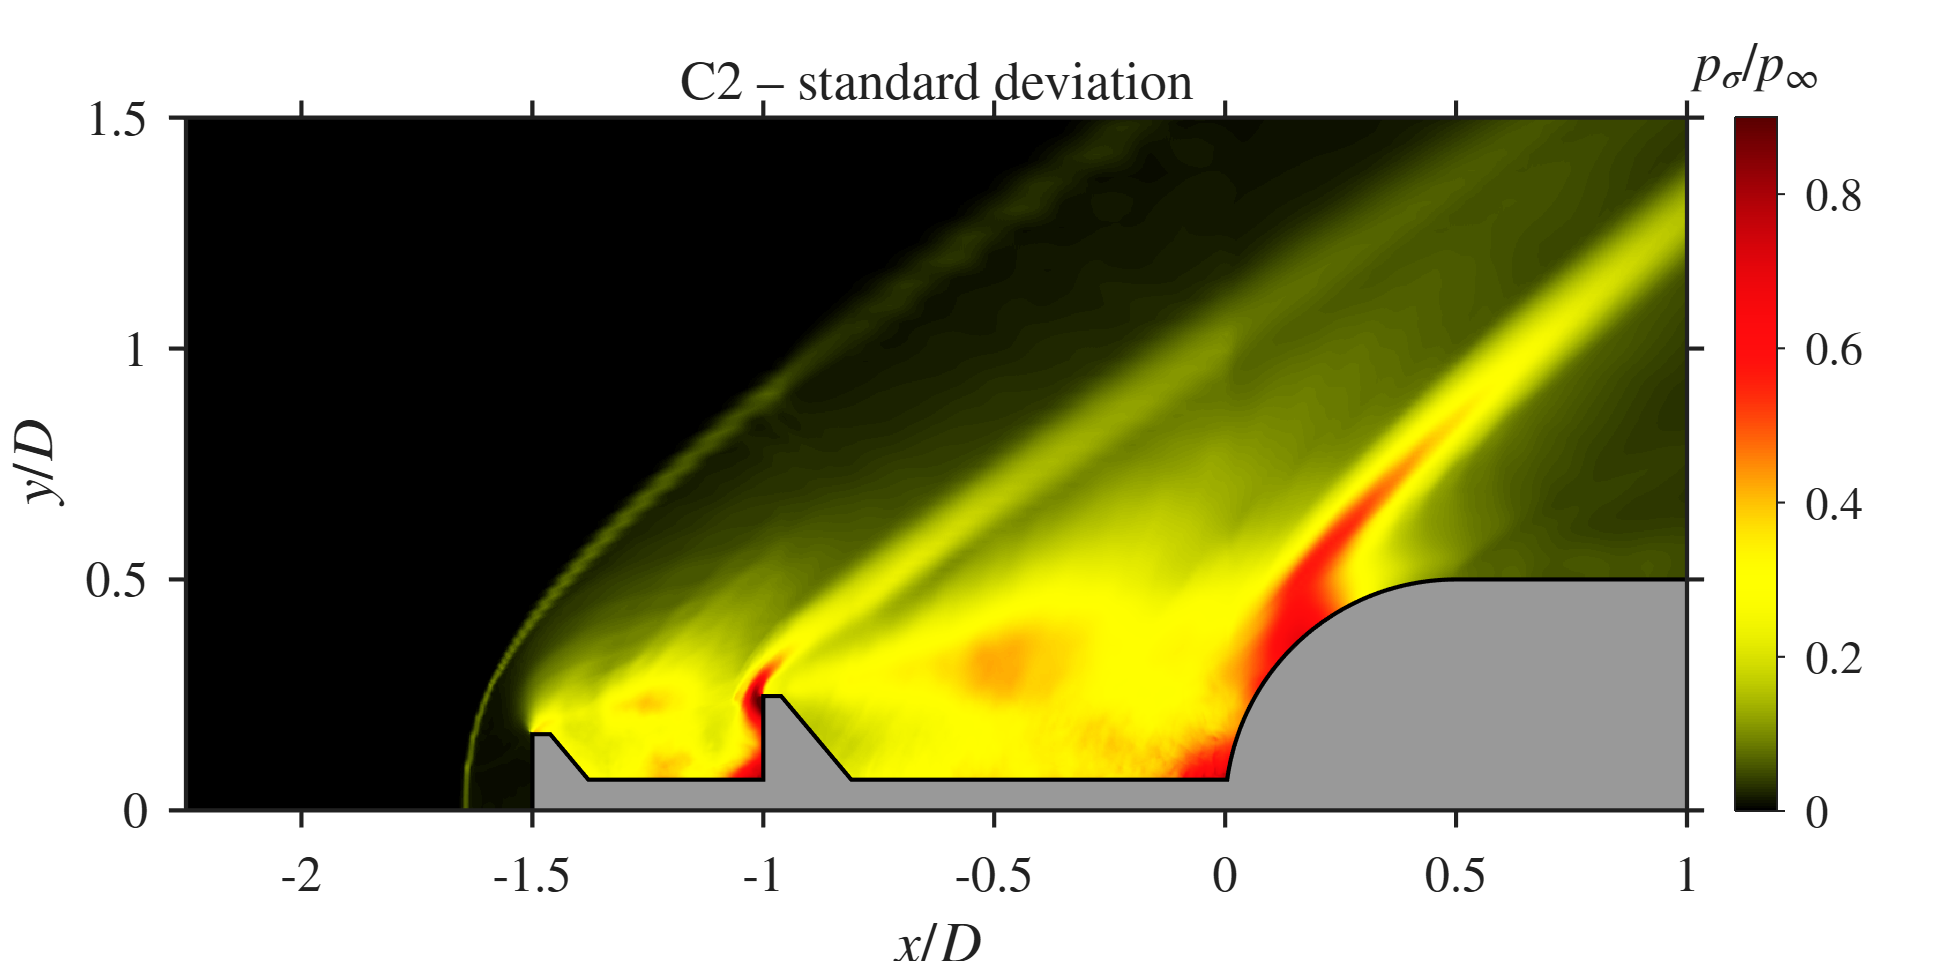
\includegraphics[width=\linewidth]{C2_std.png}\caption{C2, $\psd$}\end{subfigure}
  \caption{Gap-ratio sweep: mean pressure with streamlines (left) and pressure standard deviation (right).}
  \label{fig:gap_ms}
\end{figure}

\paragraph{Space-time behaviour.} In the $x$--$t$ diagram of C3 (Fig.~\ref{fig:gap_xt}a), Cavity 1 shows large, slow oscillations, and strong high-pressure bursts ($p/\pinf > 4$) travel from the second-disk face through Cavity 2 to the hemisphere. The reattachment line ($x_r/D = 0.196$) switches between high and low pressure with a long period, consistent with the low dominant $St = 0.25$. The pattern looks like a pulsation in which the short Cavity 2 fills and empties. C2 (Fig.~\ref{fig:gap_xt}c) looks more like SA: Cavity 1 adds little structure, Cavity 2 shows convecting streaks, and the reattachment line ($x_r/D = 0.226$) oscillates at $St = 0.56$.

\begin{figure}[htbp]
  \centering
  \begin{subfigure}{0.325\textwidth}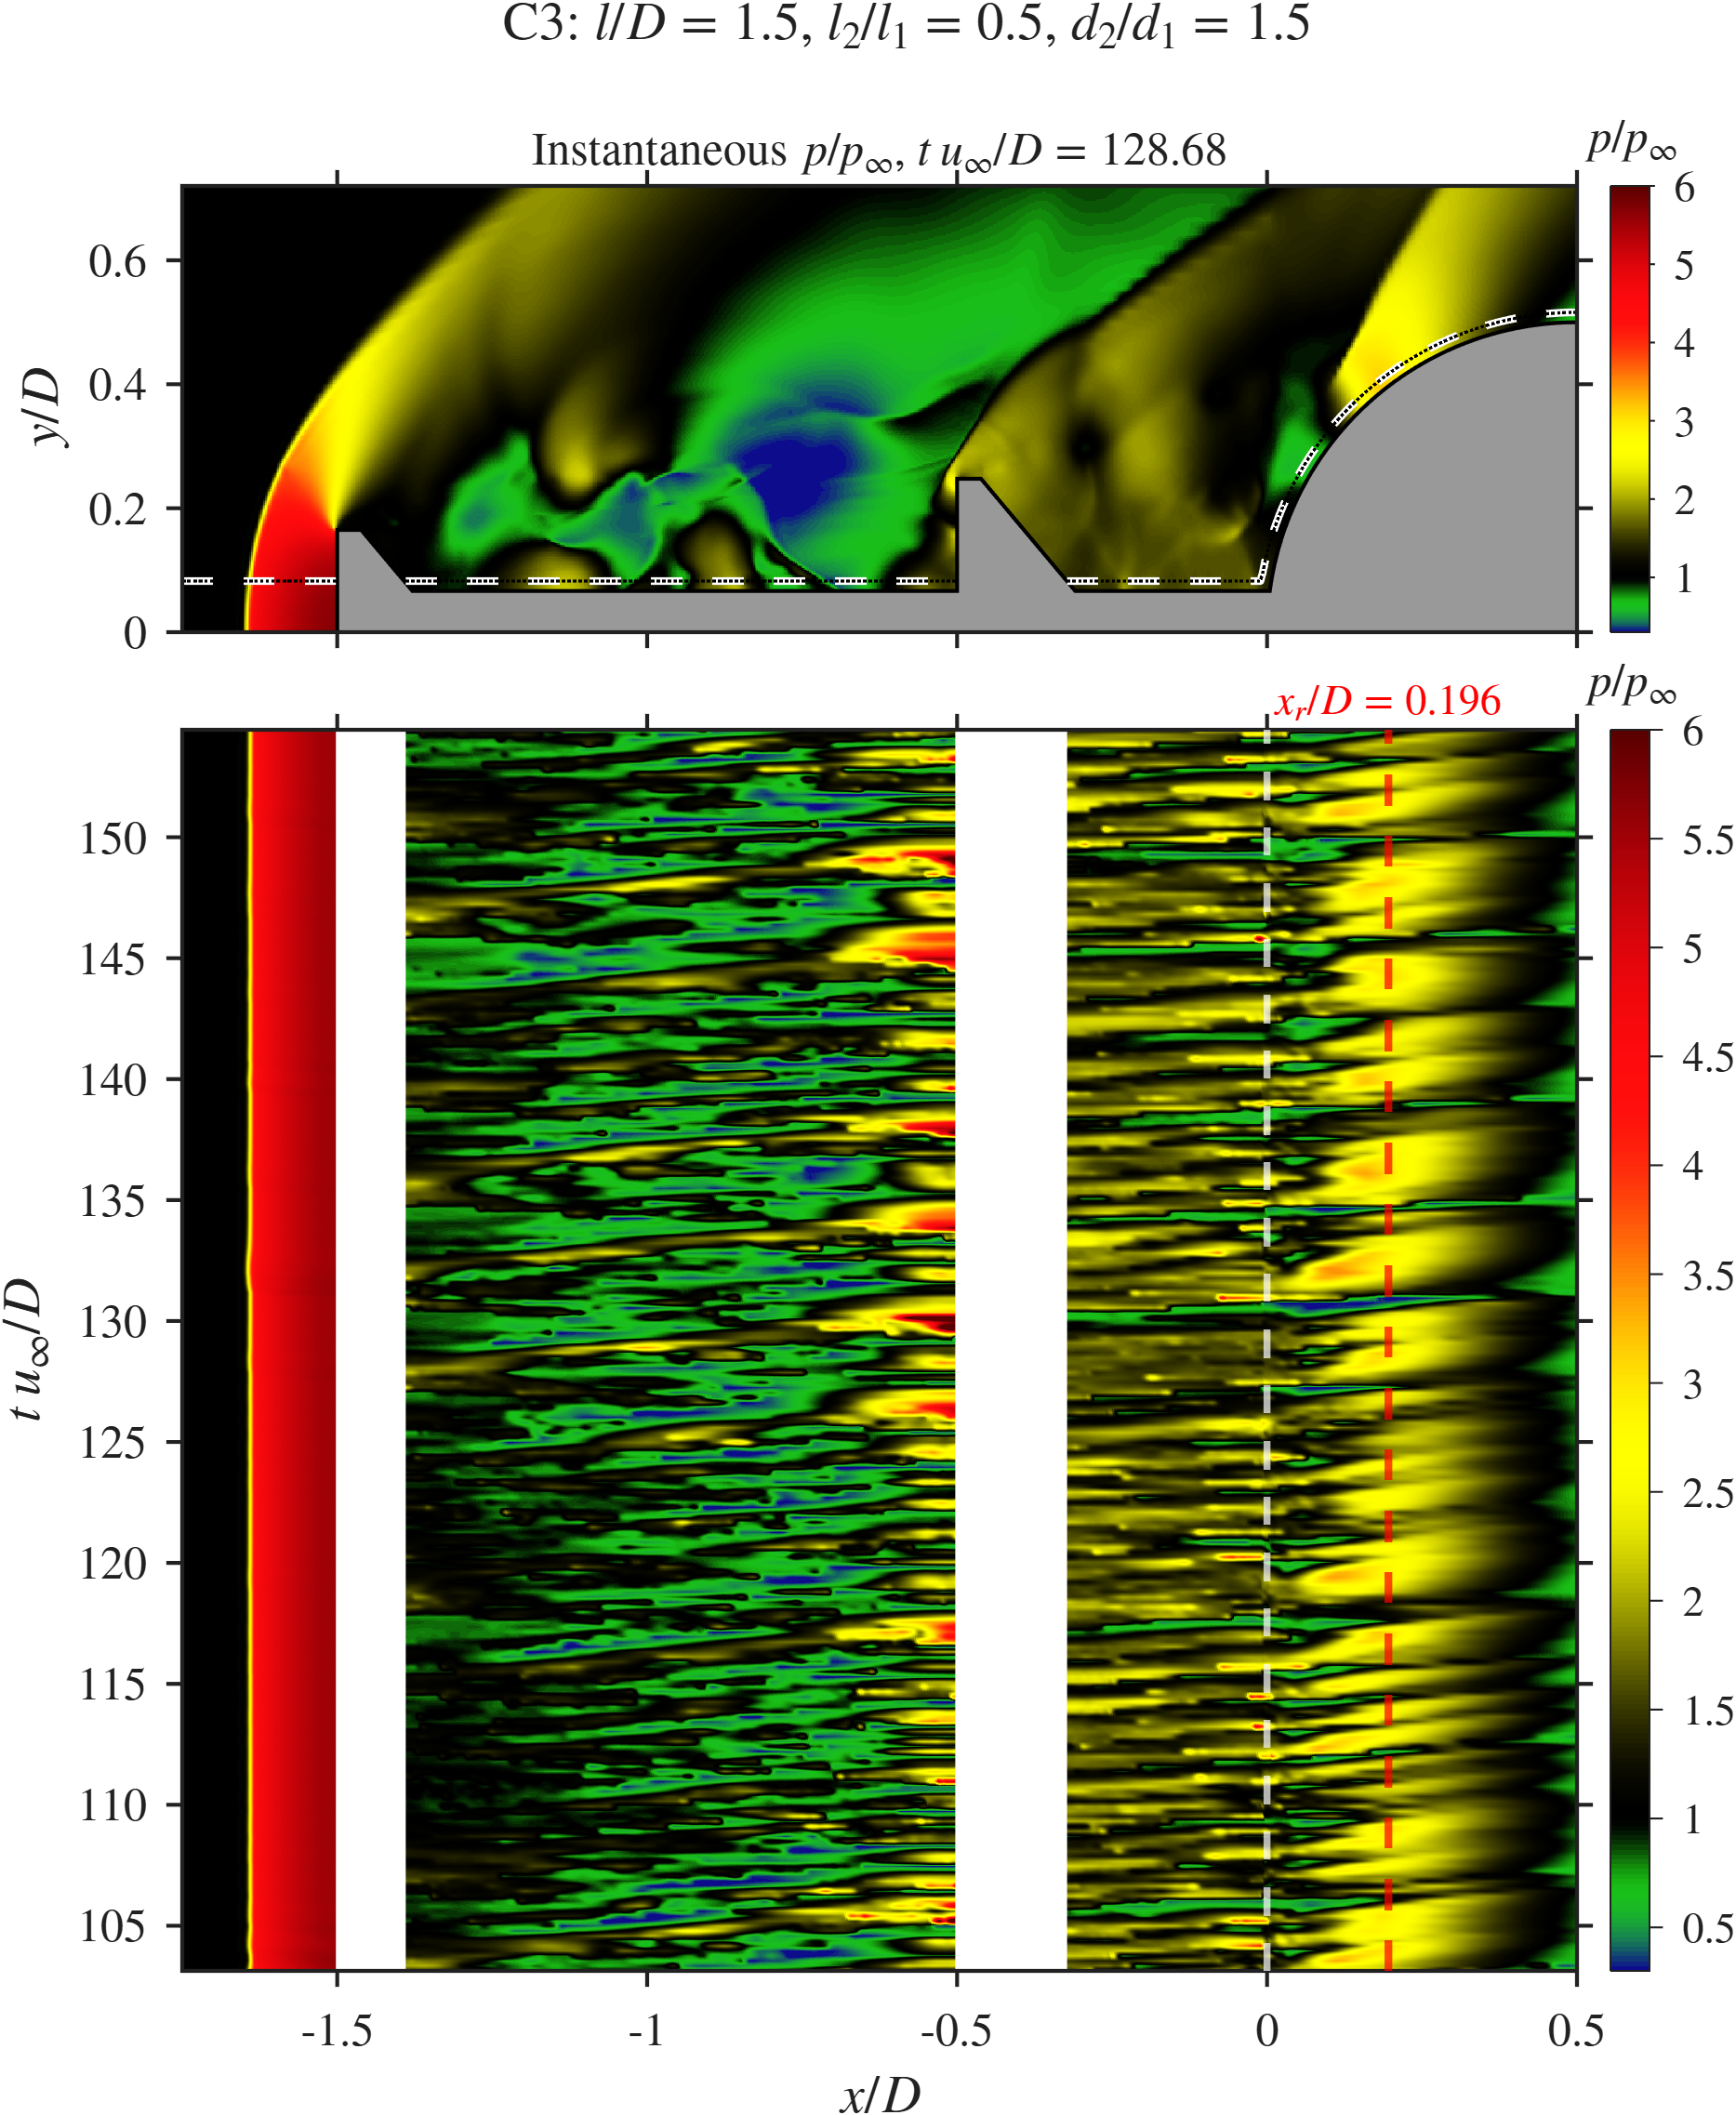
\includegraphics[width=\linewidth]{C3_xt.png}\caption{C3}\end{subfigure}
  \begin{subfigure}{0.325\textwidth}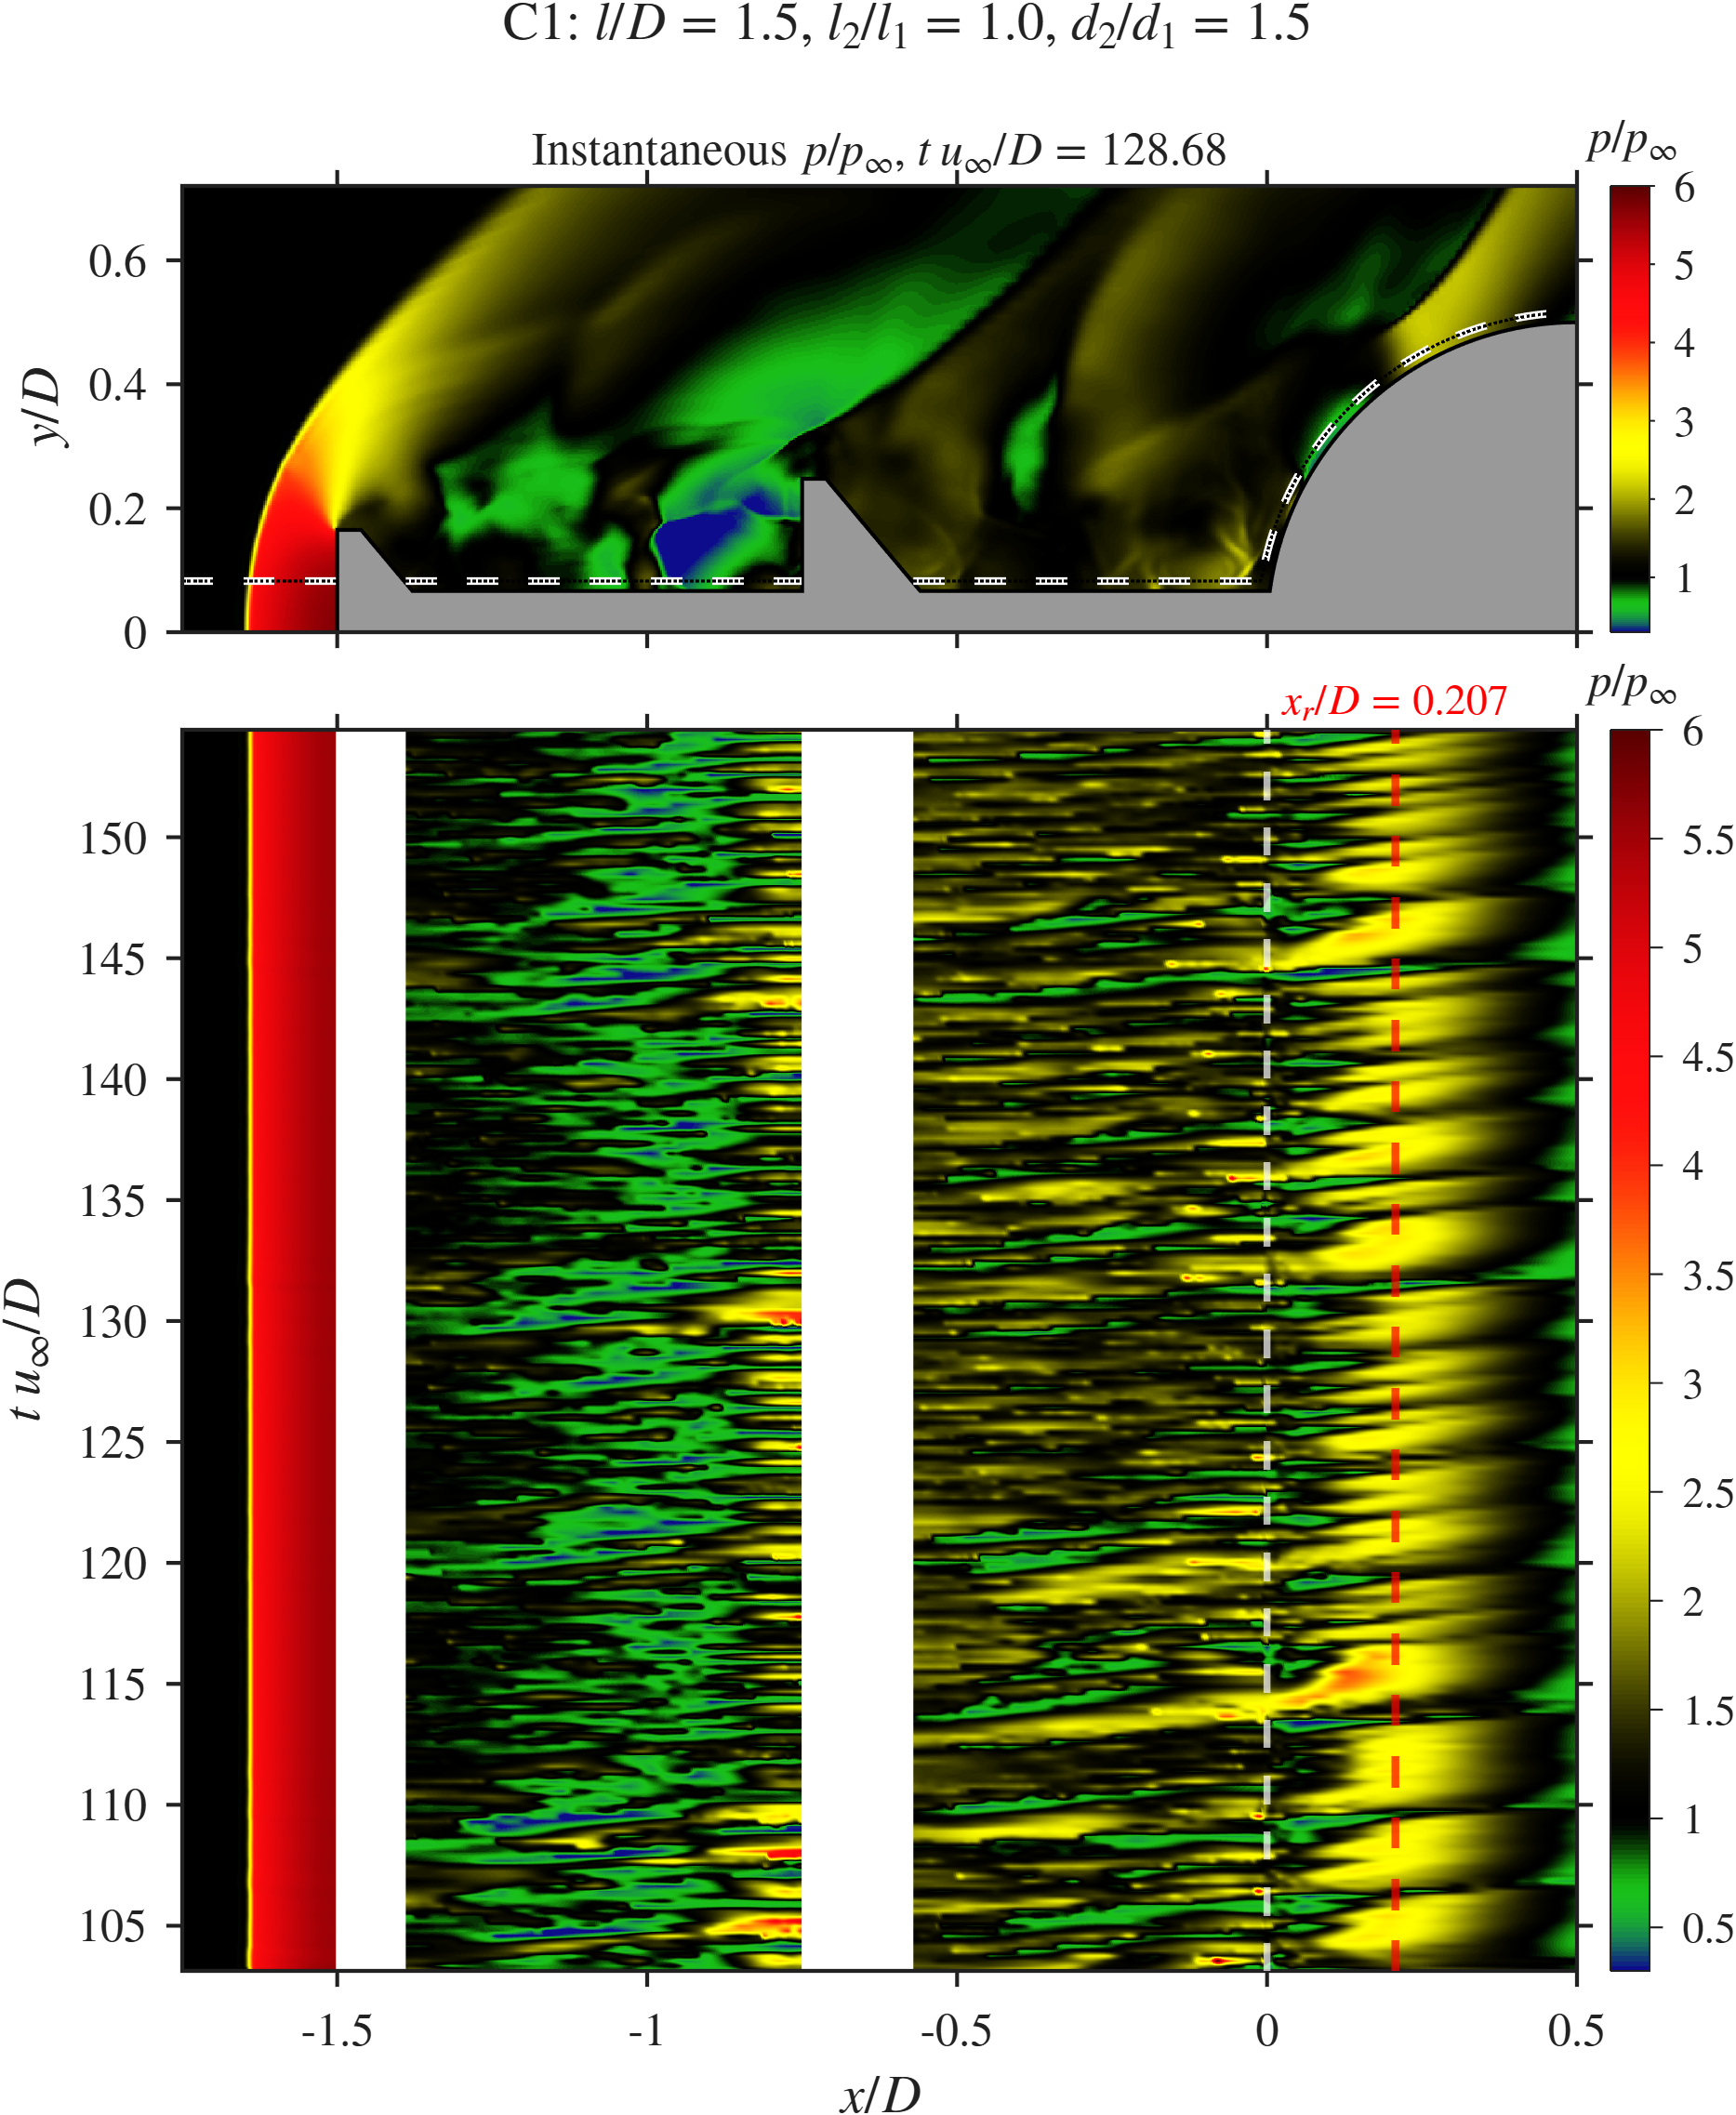
\includegraphics[width=\linewidth]{C1_xt.png}\caption{C1}\end{subfigure}
  \begin{subfigure}{0.325\textwidth}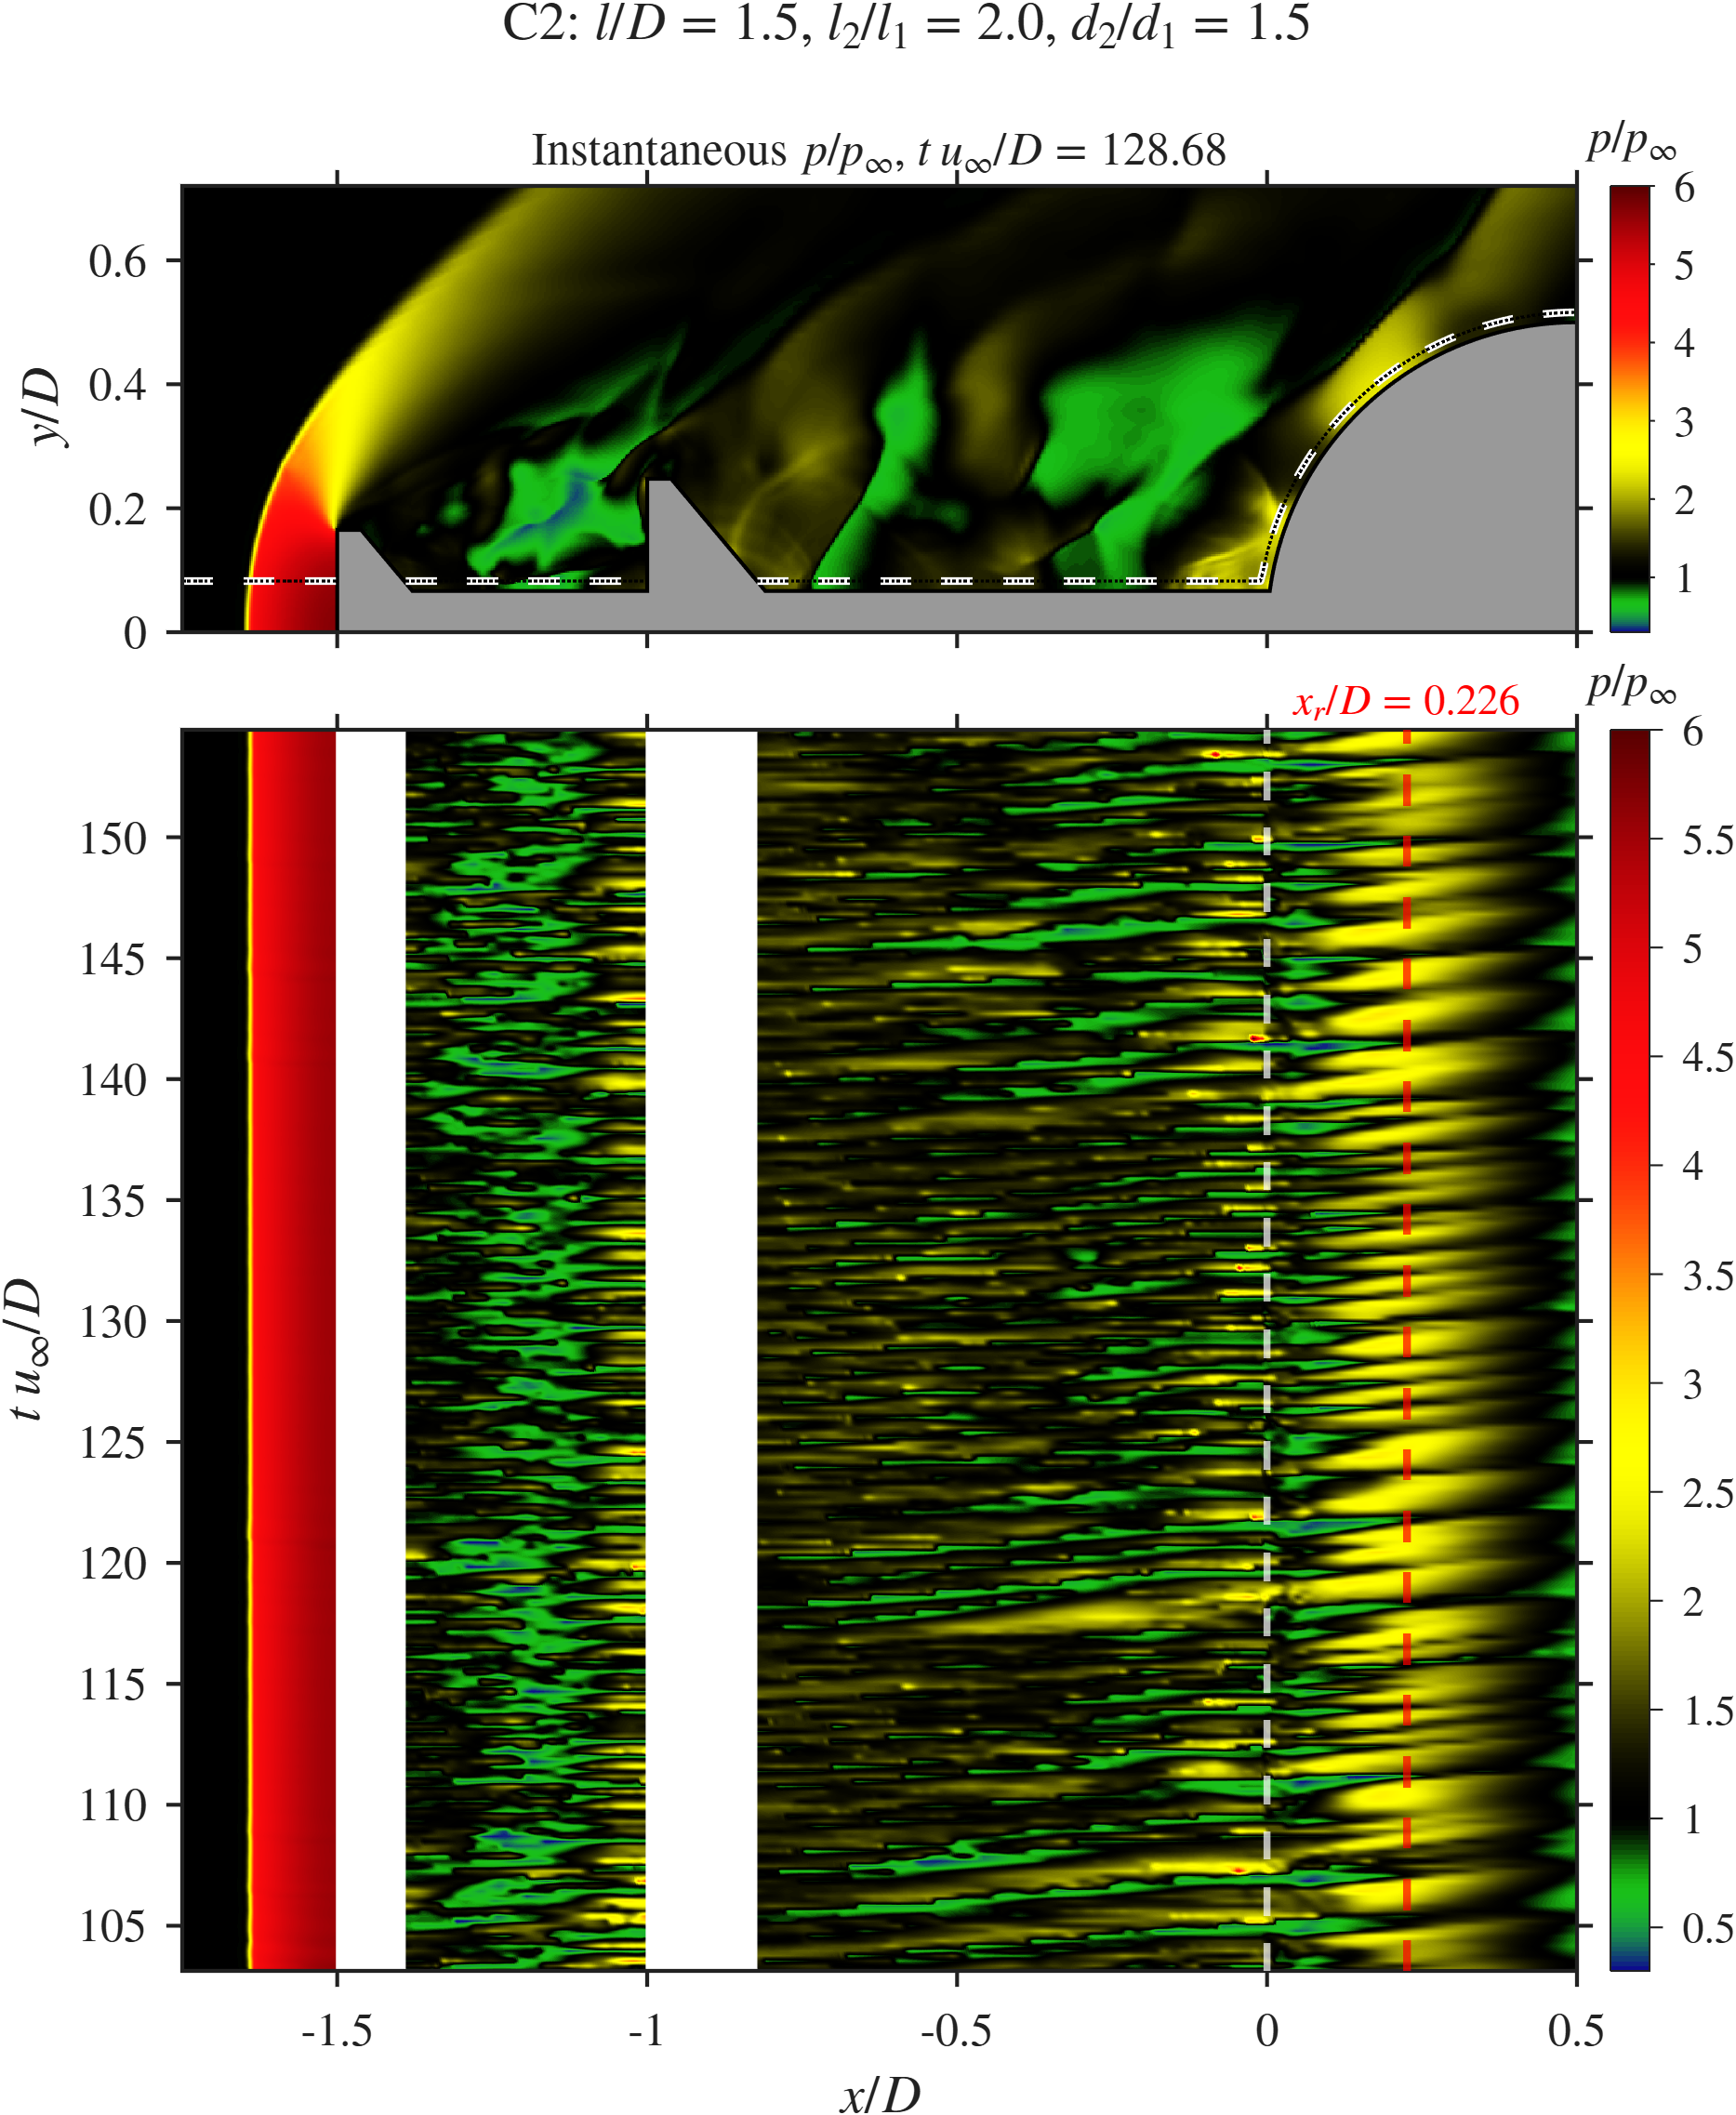
\includegraphics[width=\linewidth]{C2_xt.png}\caption{C2}\end{subfigure}
  \caption{Gap-ratio sweep: $x$--$t$ diagrams of $p/\pinf$ along the probe line.}
  \label{fig:gap_xt}
\end{figure}

The $x$--$f$ diagrams (Fig.~\ref{fig:gap_xf}) show how the gap changes the frequency of each cavity. In C3 the disk-face band drops to $St \approx 0.53$, and Cavity 2 carries $St \approx 0.88$. In C2 both cavities share the same band at $St \approx 1.12$, so the two cavities are locked to one frequency.

\begin{figure}[htbp]
  \centering
  \begin{subfigure}{0.325\textwidth}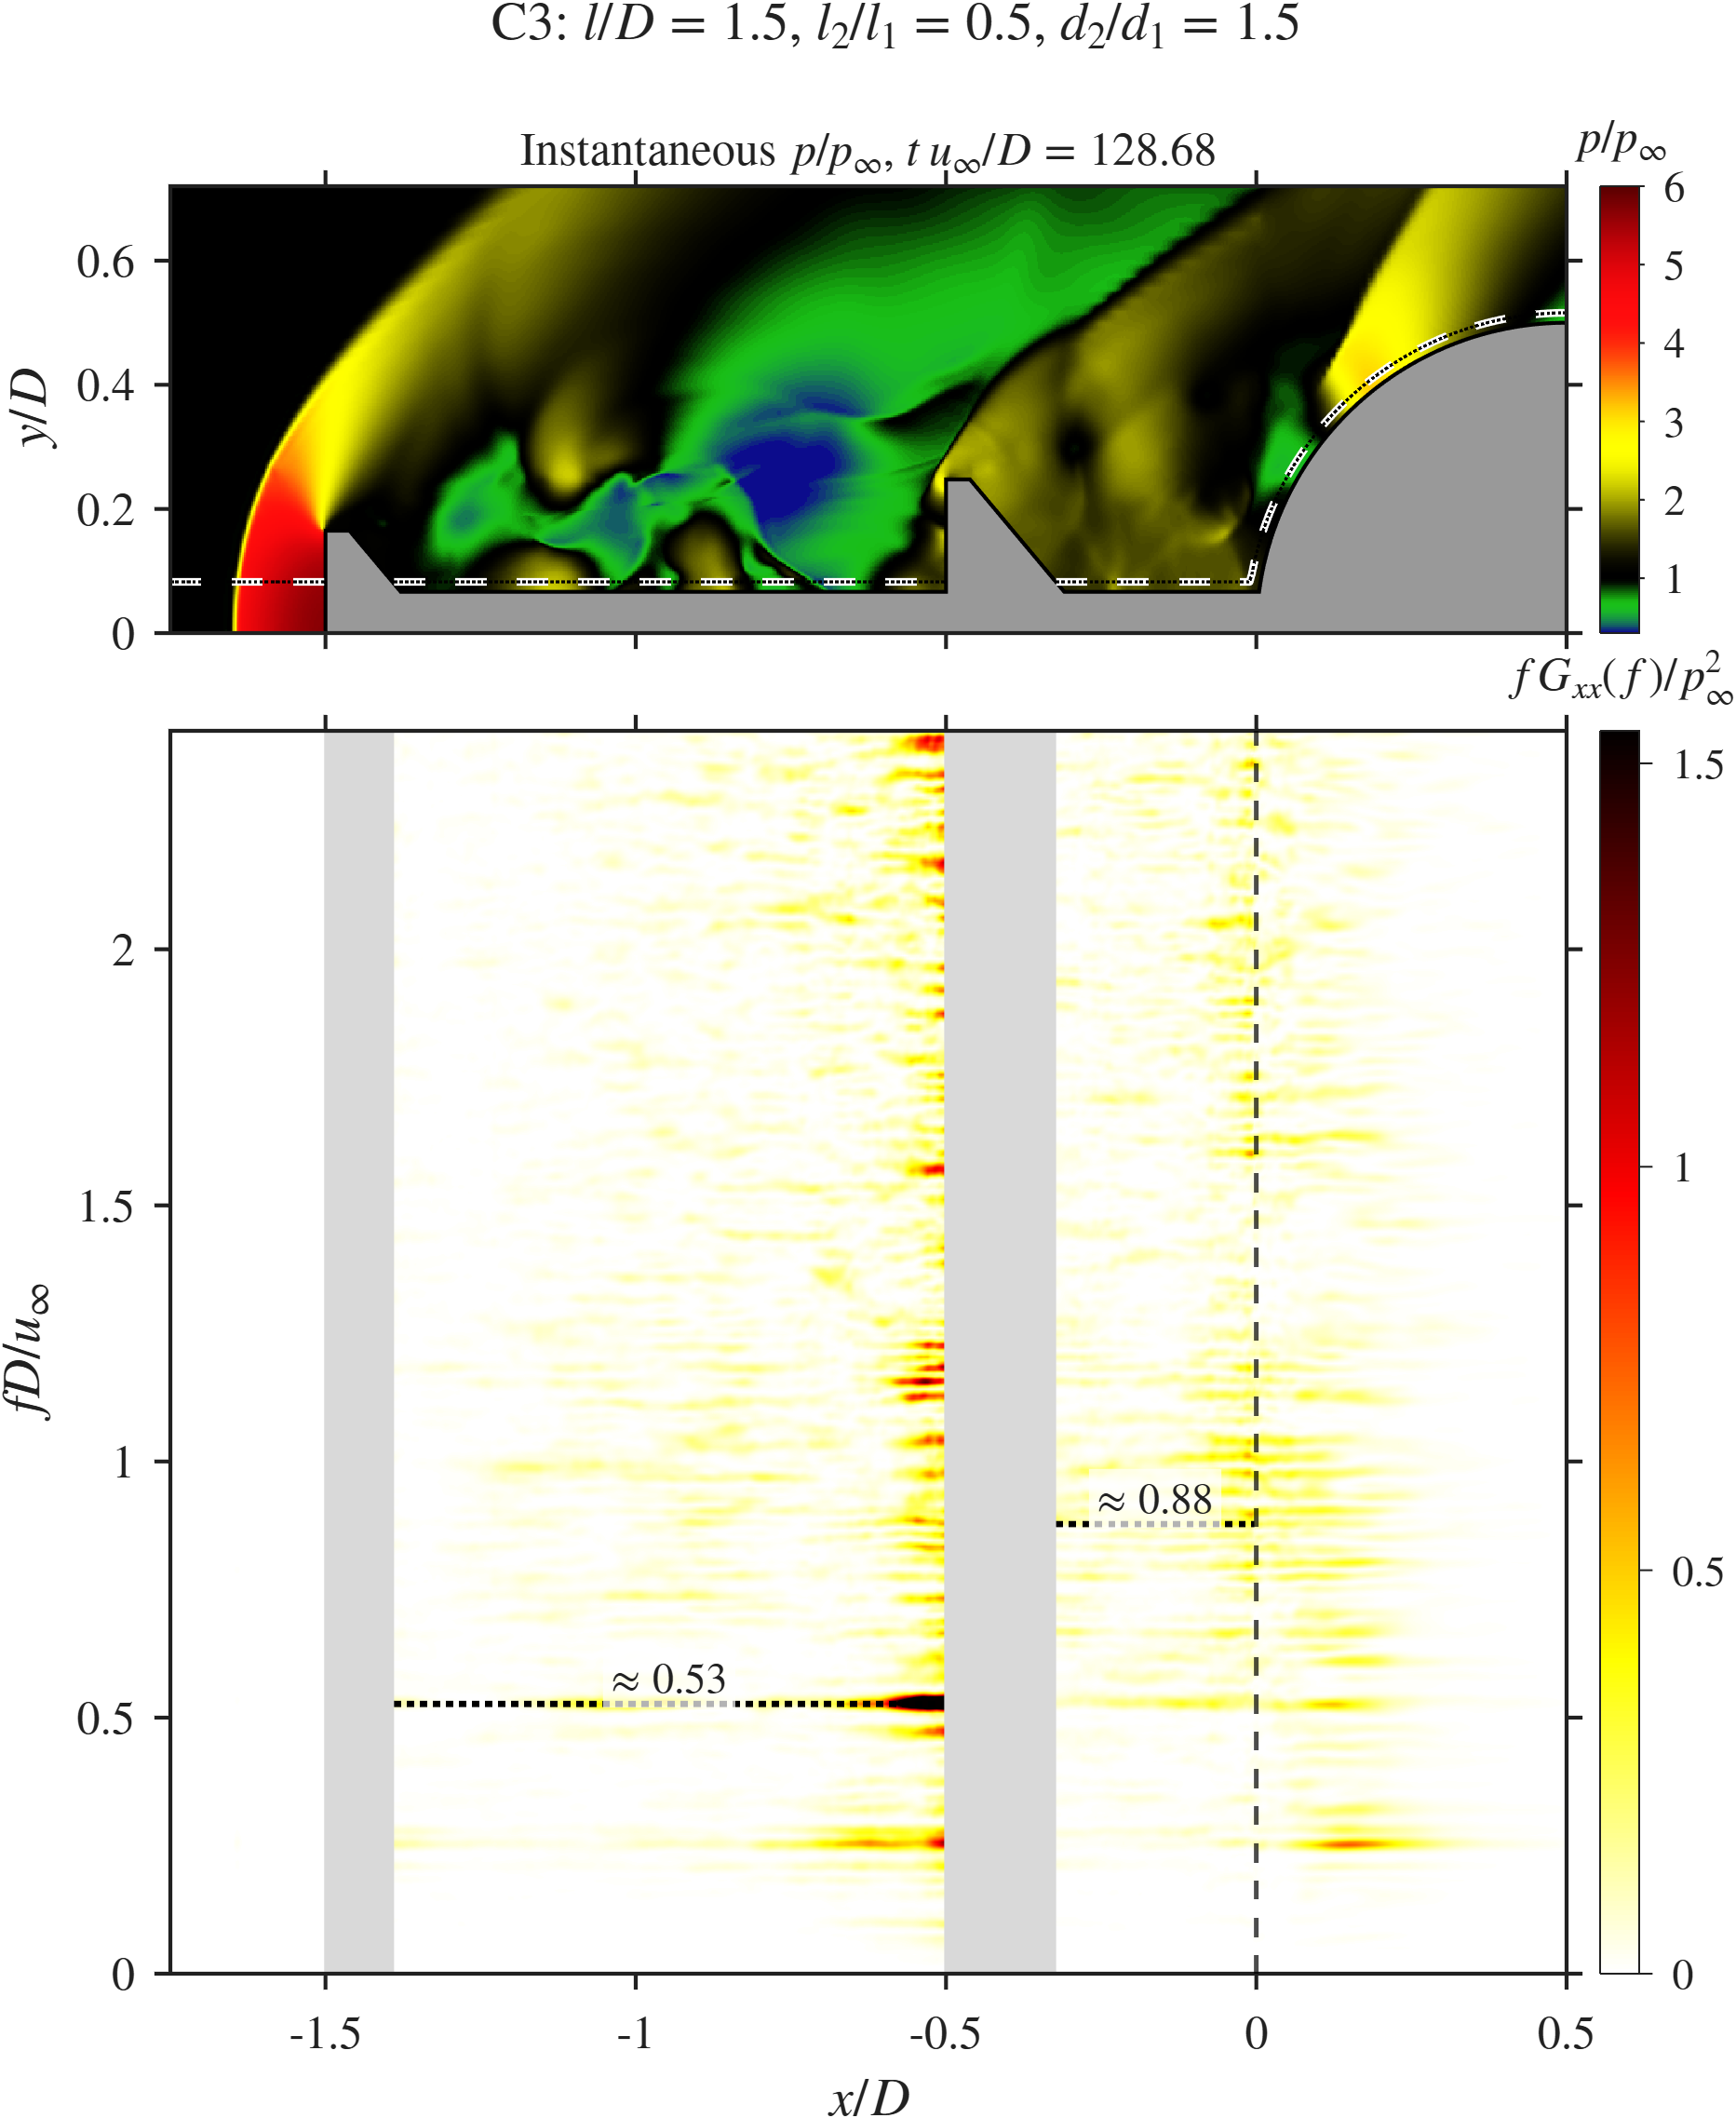
\includegraphics[width=\linewidth]{C3_xf.png}\caption{C3}\end{subfigure}
  \begin{subfigure}{0.325\textwidth}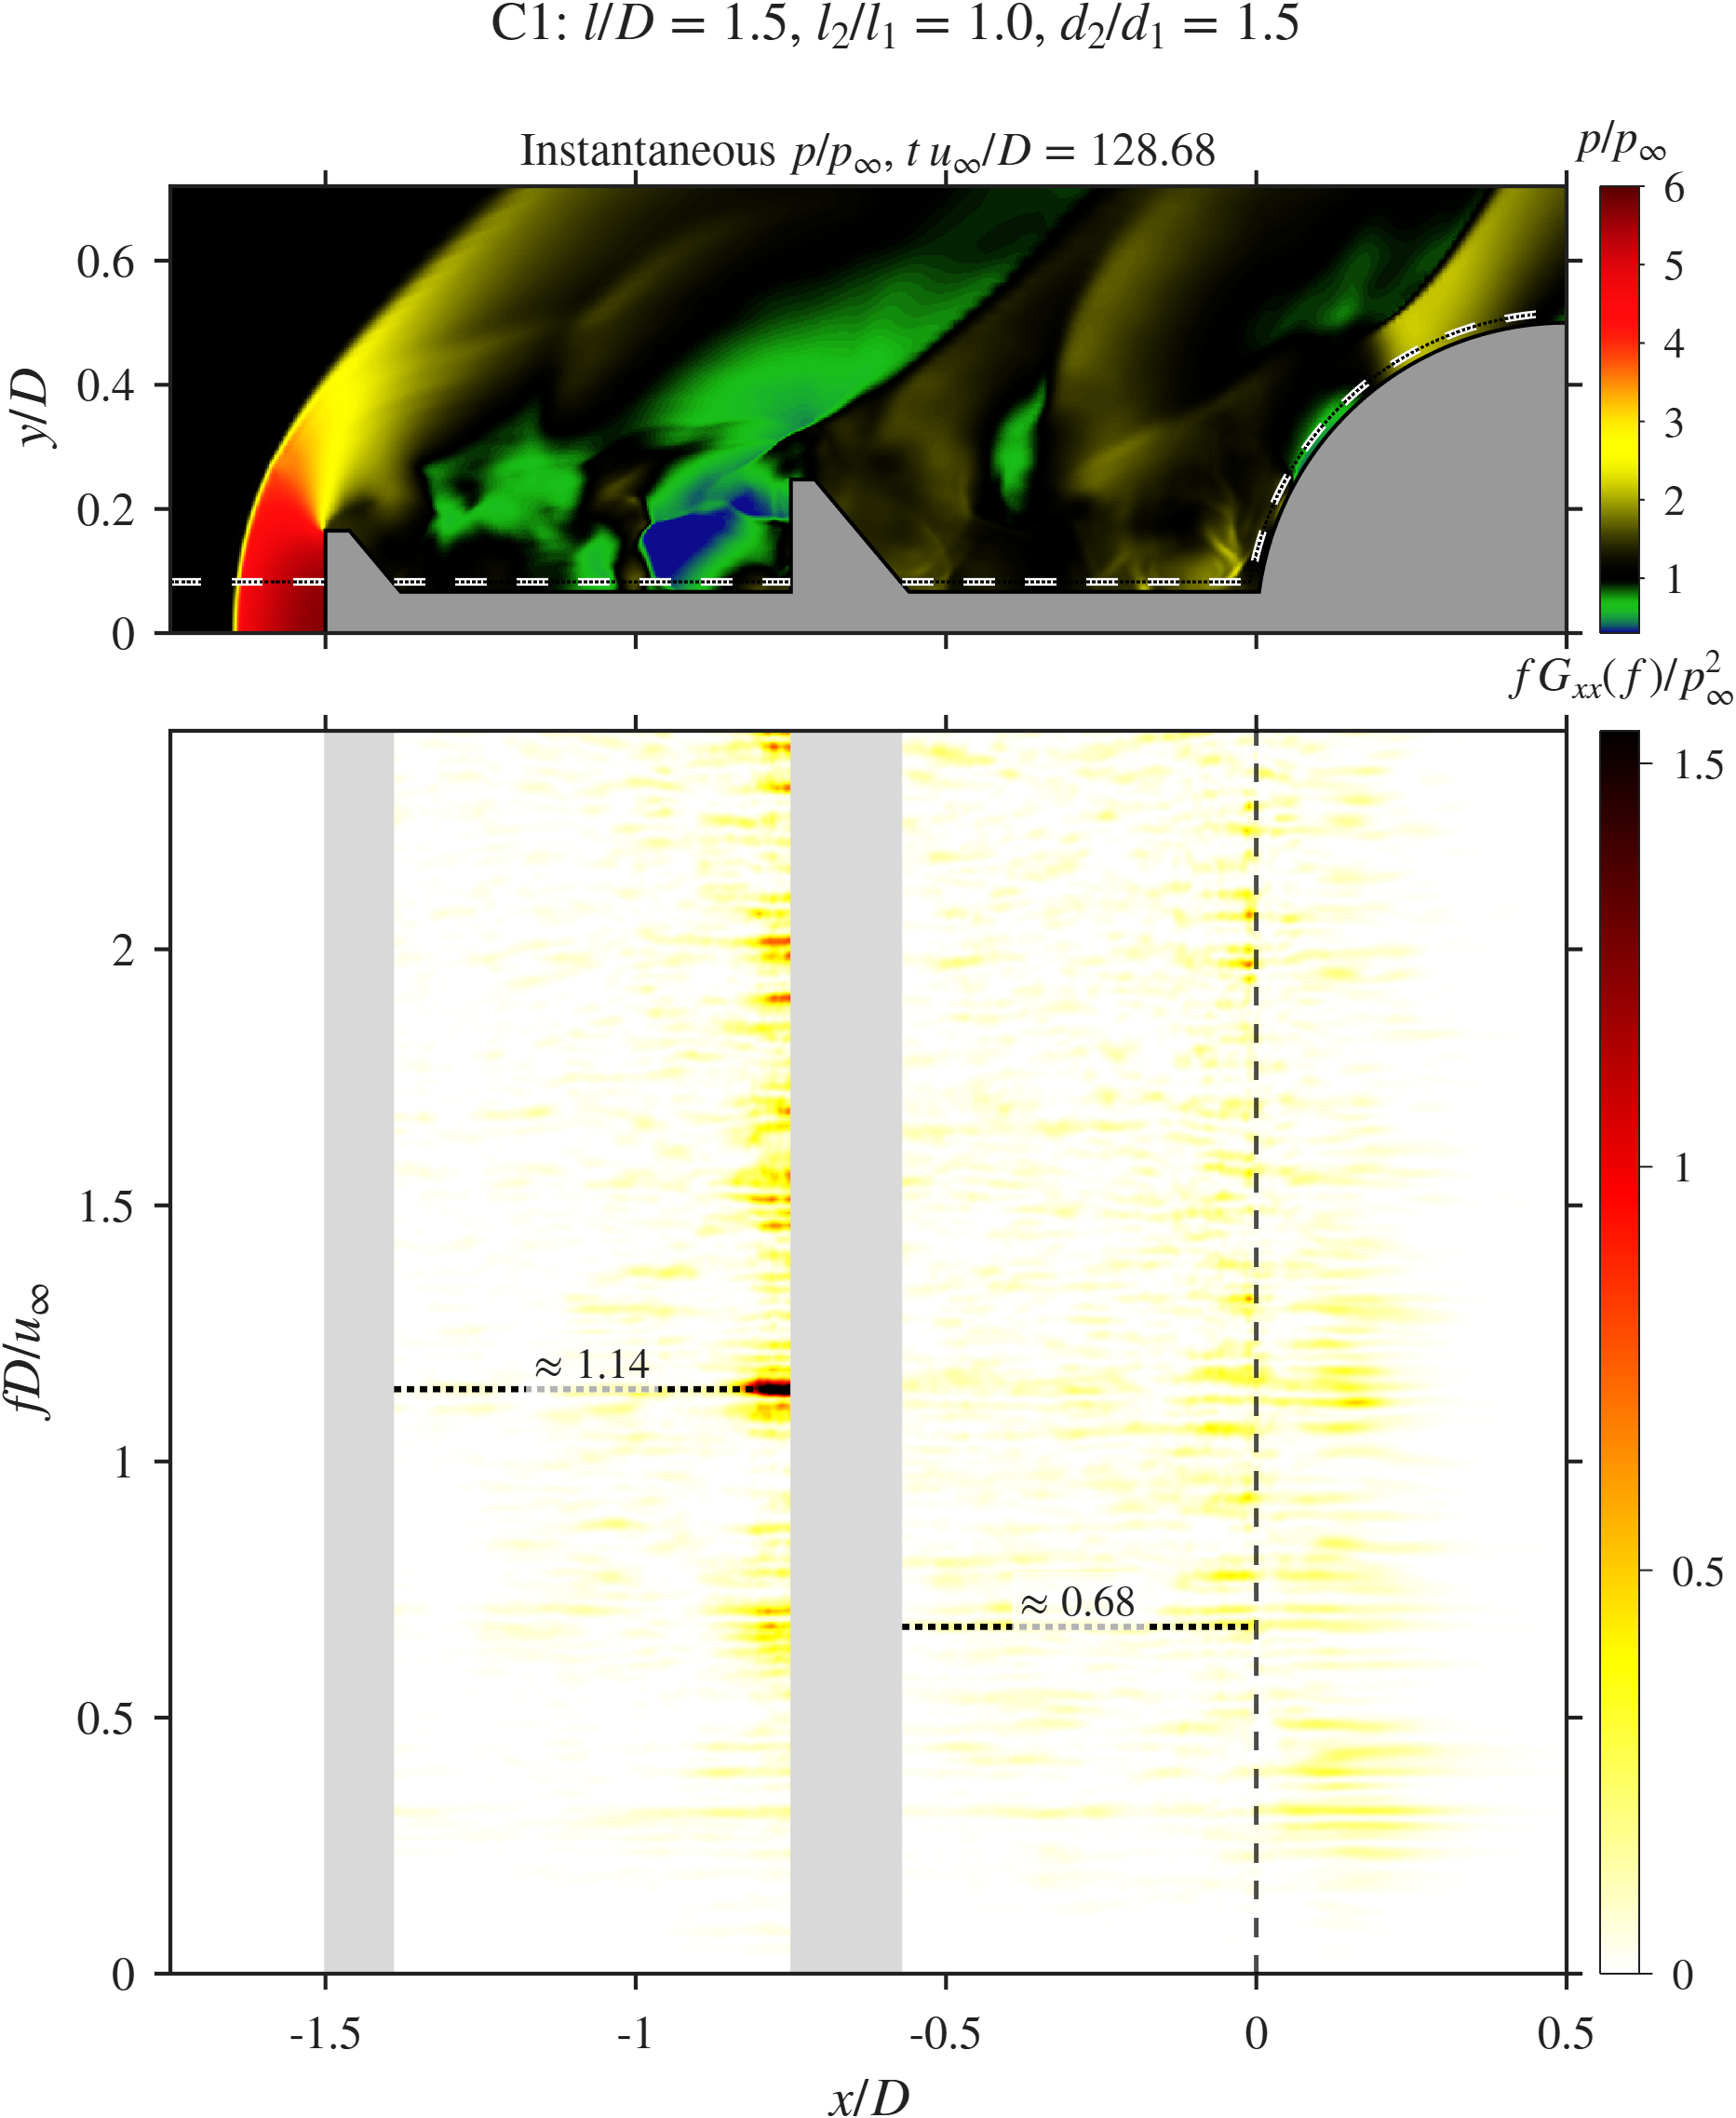
\includegraphics[width=\linewidth]{C1_xf.png}\caption{C1}\end{subfigure}
  \begin{subfigure}{0.325\textwidth}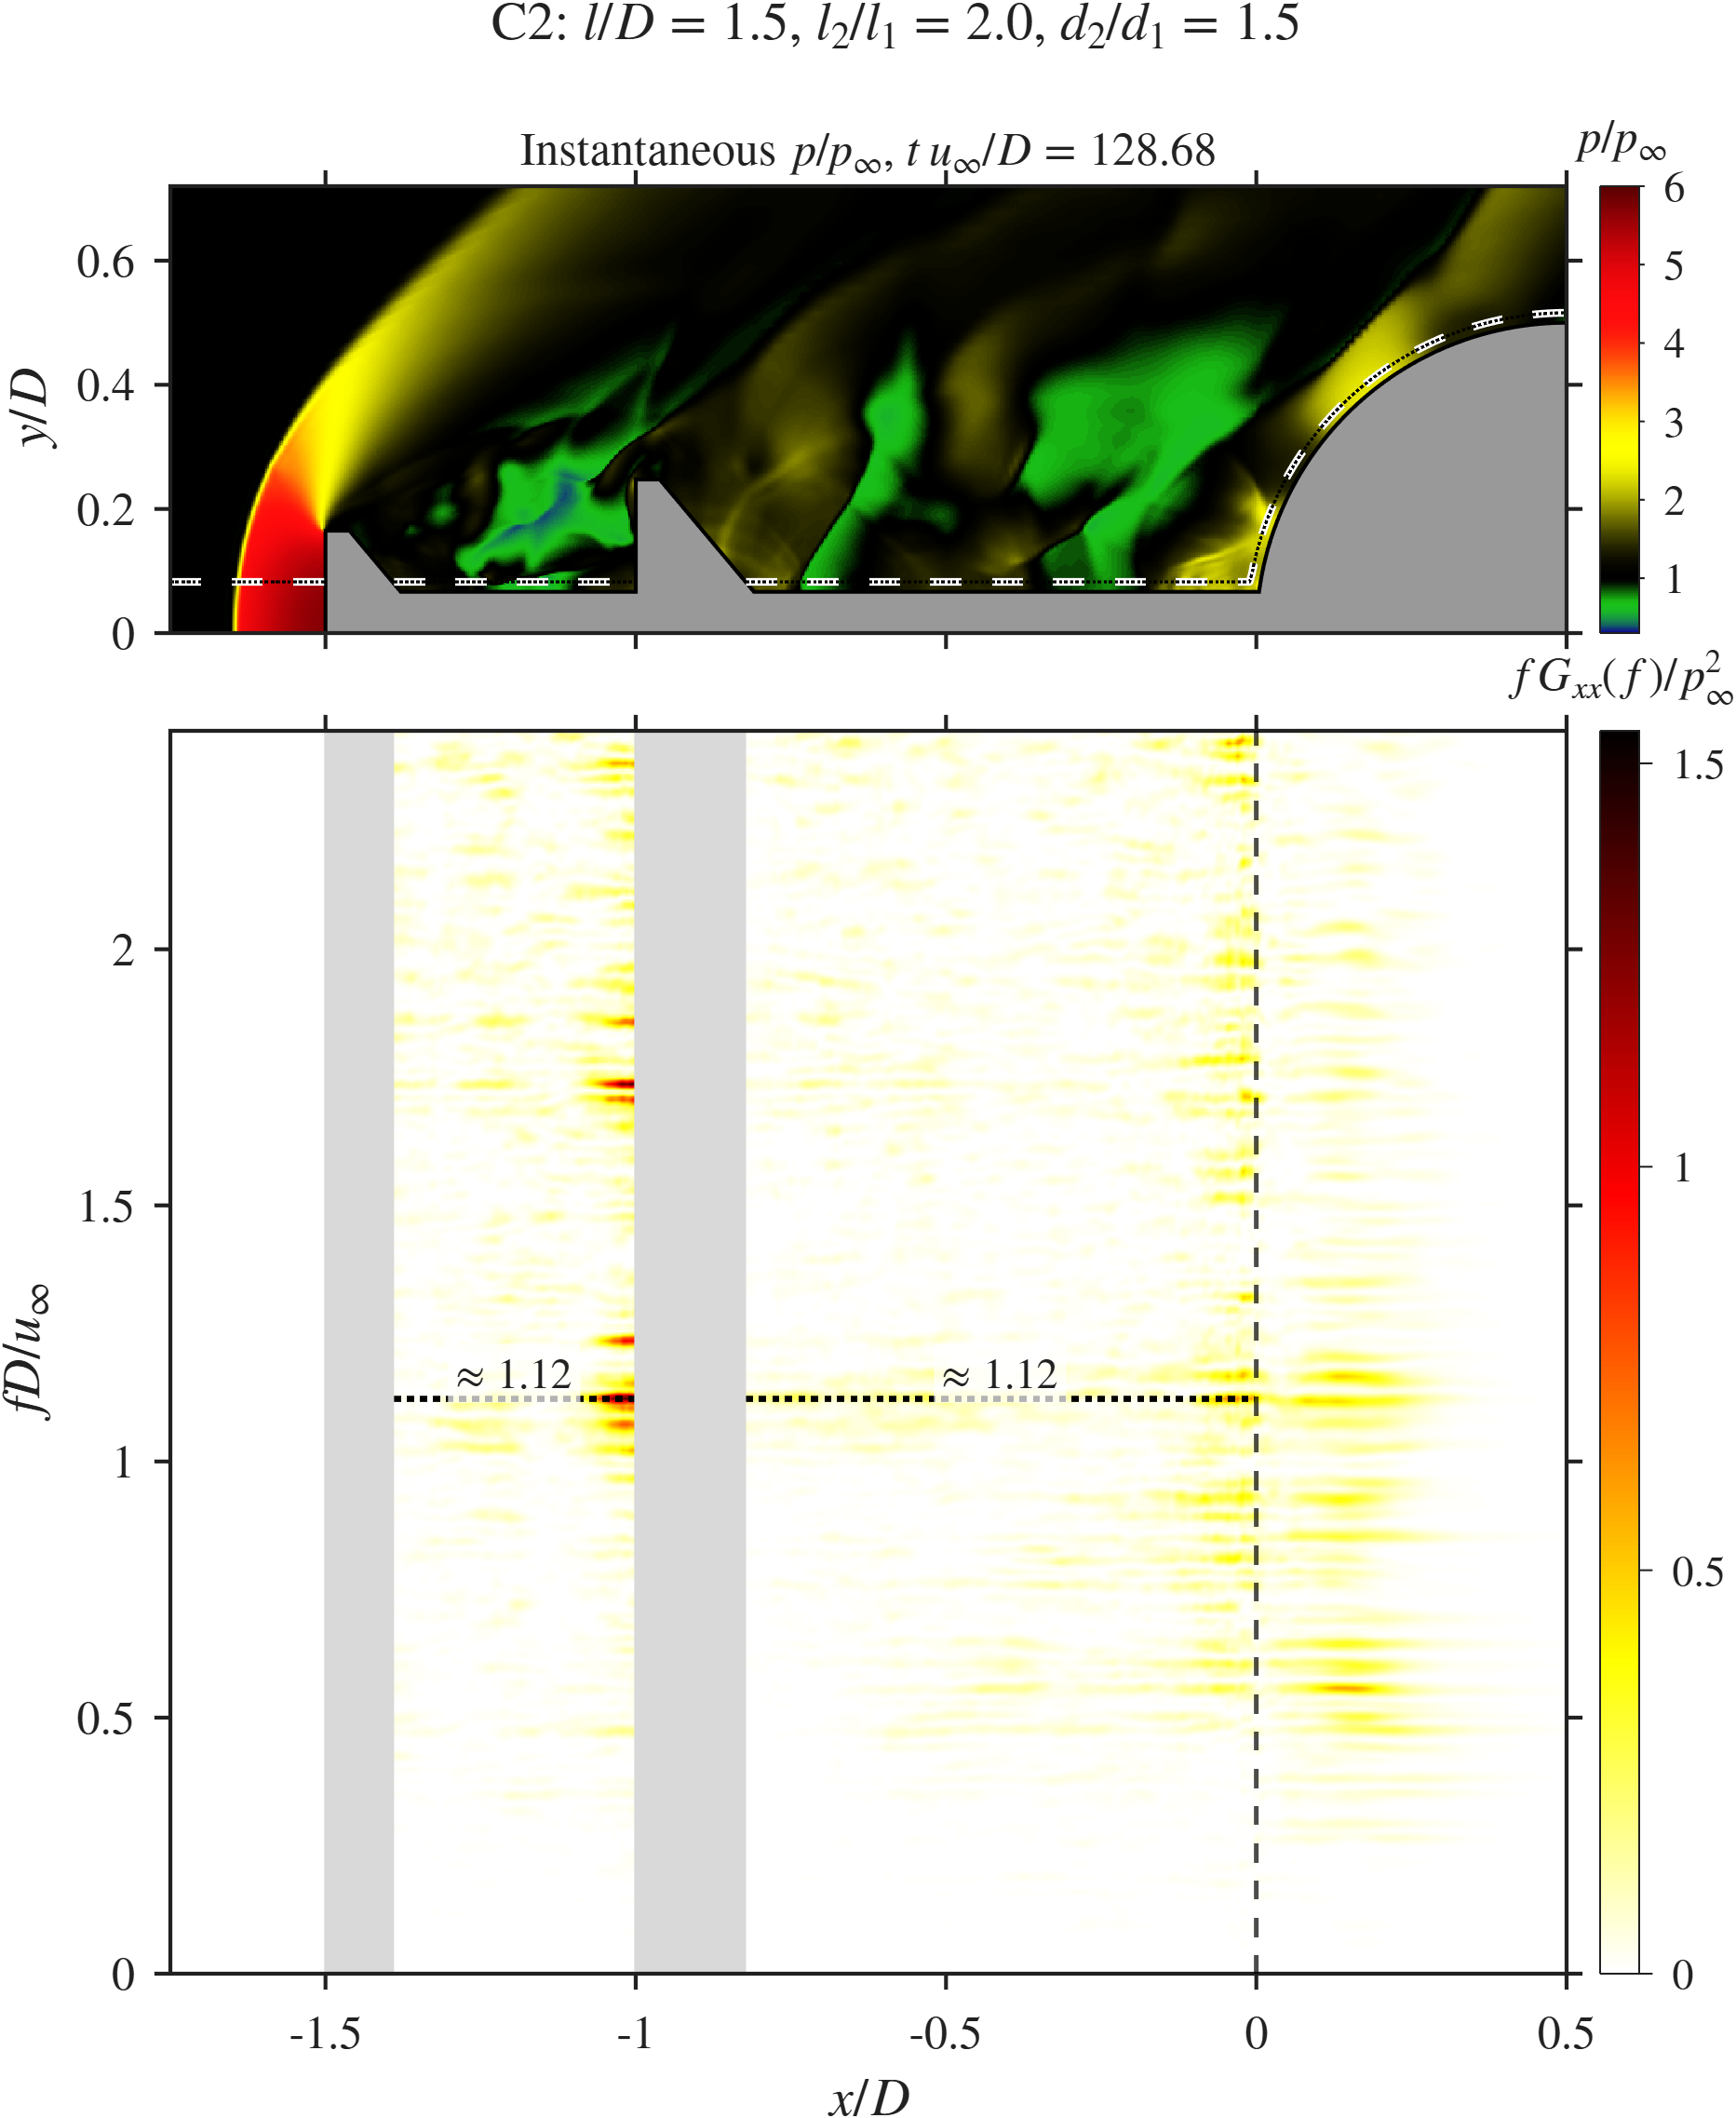
\includegraphics[width=\linewidth]{C2_xf.png}\caption{C2}\end{subfigure}
  \caption{Gap-ratio sweep: $x$--$f$ diagrams along the probe line.}
  \label{fig:gap_xf}
\end{figure}

\paragraph{Probe signals and spectra.} Figure~\ref{fig:gap_sig} shows the signals and spectra. C3 has its peak at a low $St = 0.25$ with $\Pi \approx 0.61$, the highest peak of the three cases, though still about 83\% below SA. The low frequency and the strong peak fit a pulsation-like process in which the short Cavity 2 exchanges mass with the outer flow at a slow rate. C1 has the broad spectrum described above (peak at $St = 1.12$, $\Pi \approx 0.37$). C2 has a peak at $St = 0.56$ with $\Pi \approx 0.50$, which sits between the SA tone and the broad C1 spectrum.

The pressure and drag frequencies also separate in this sweep. In C1 they are close ($St = 1.12$ and 1.14). In C2 they are 0.56 and 0.89, and in C3 they are 0.25 and 0.53. The C3 drag peak (0.53) matches the disk-face band of its $x$--$f$ diagram ($St \approx 0.53$), so in C3 the drag follows the impingement on the second disk while the shoulder probe follows the slower pulsation. Drag integrates pressure over the disks, the stem and the hemisphere, so it can be set by a different part of the flow than a single shoulder probe.

\begin{figure}[htbp]
  \centering
  \begin{subfigure}{\textwidth}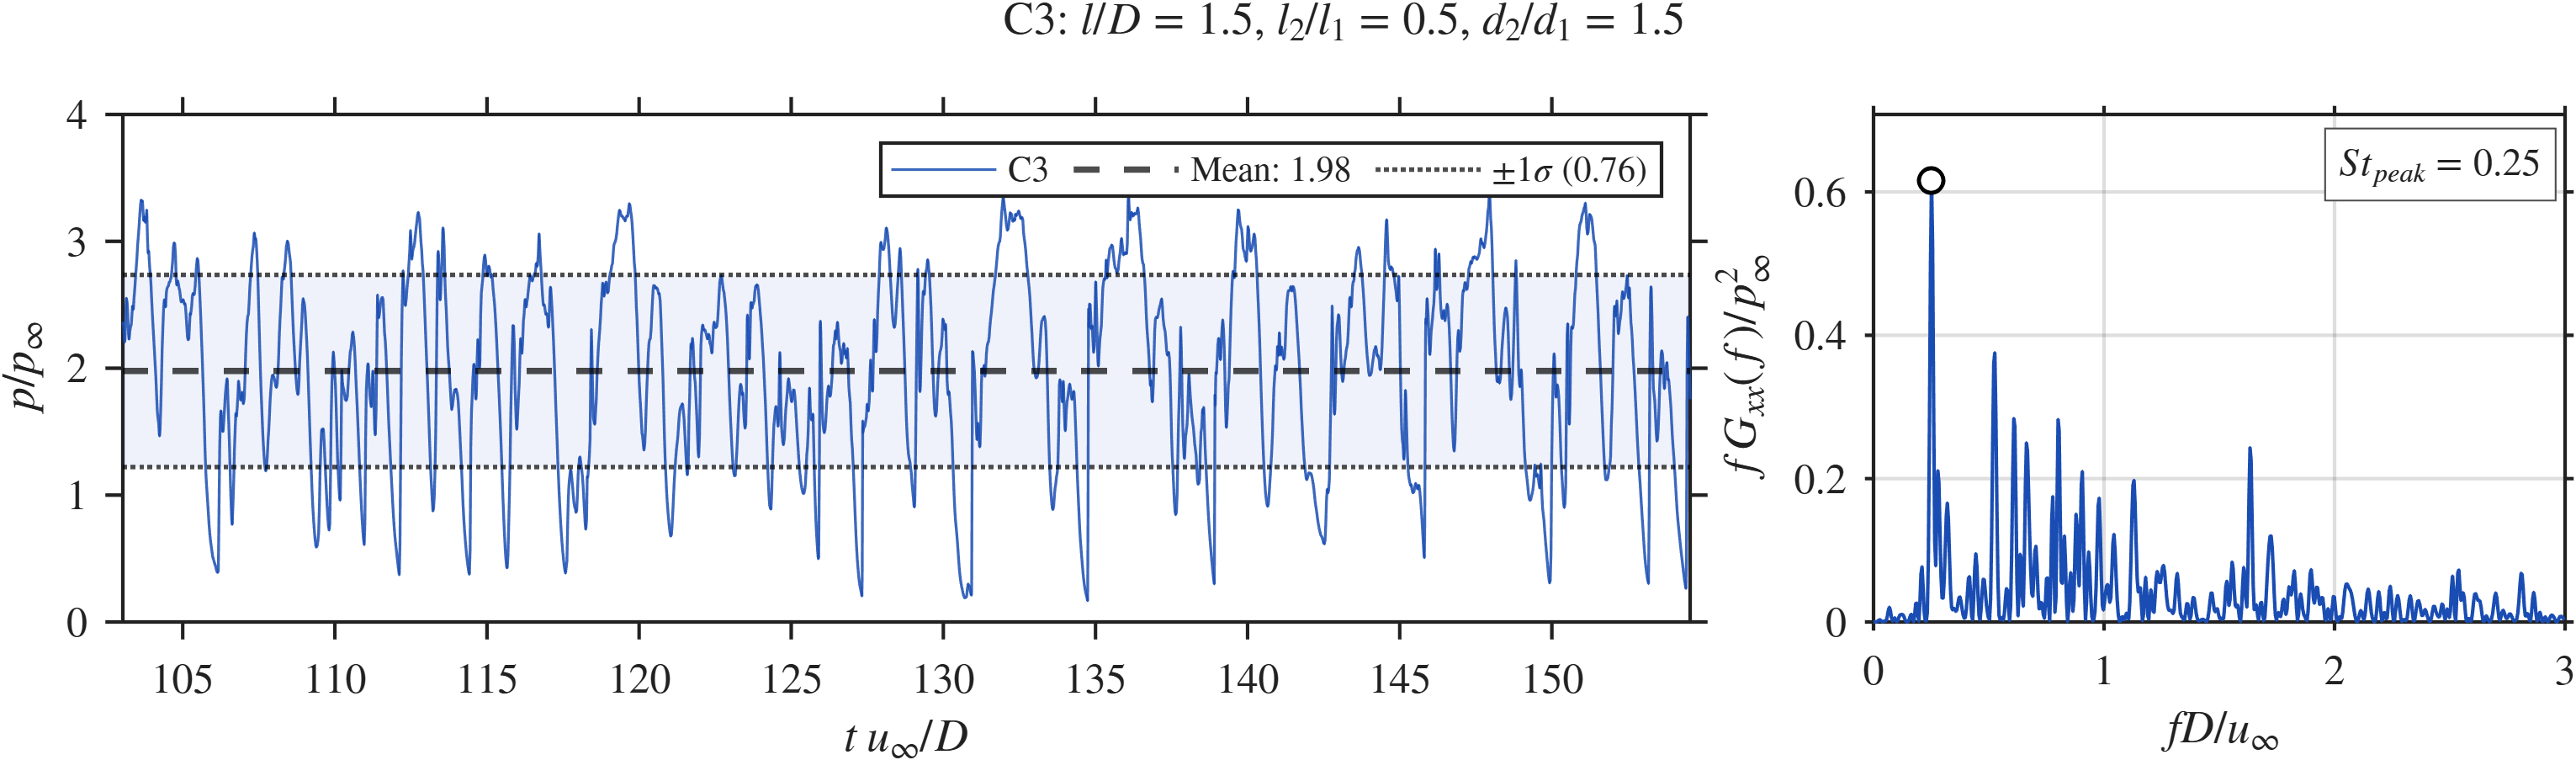
\includegraphics[width=\linewidth]{C3_psig.png}\caption{C3, pressure}\end{subfigure}\\
  \begin{subfigure}{\textwidth}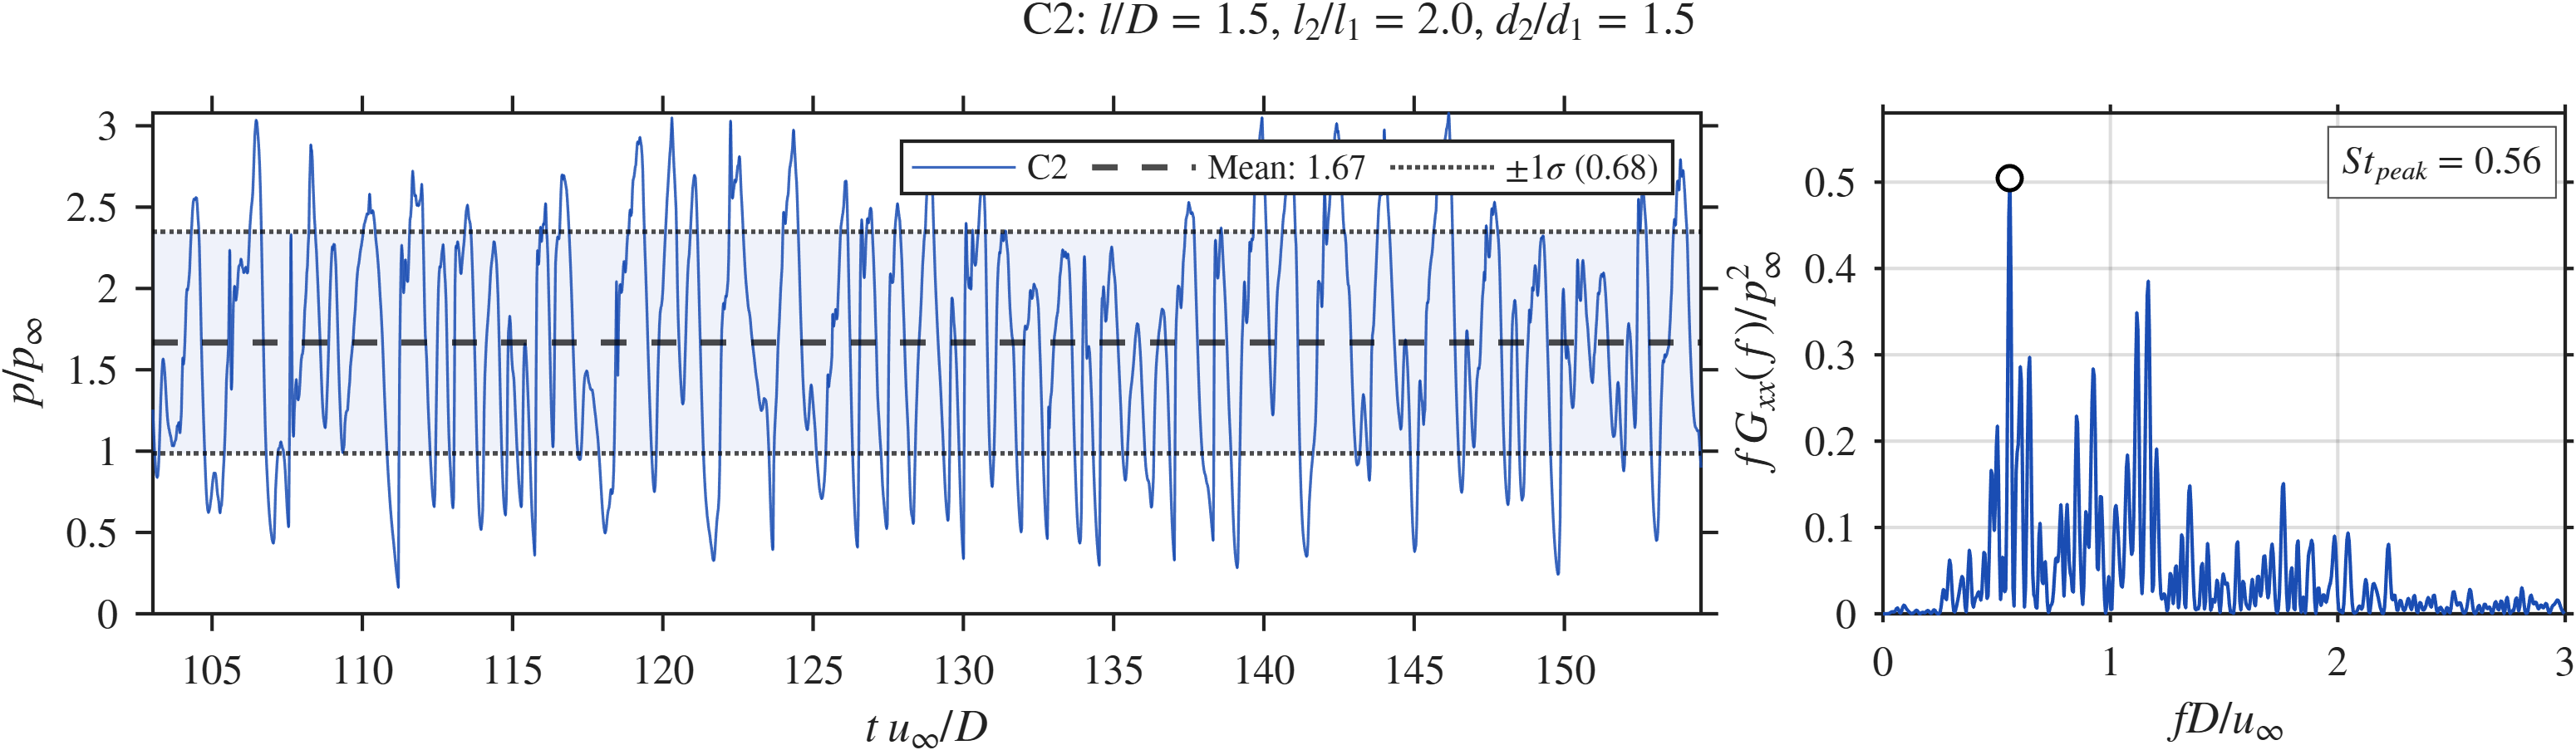
\includegraphics[width=\linewidth]{C2_psig.png}\caption{C2, pressure}\end{subfigure}\\
  \begin{subfigure}{\textwidth}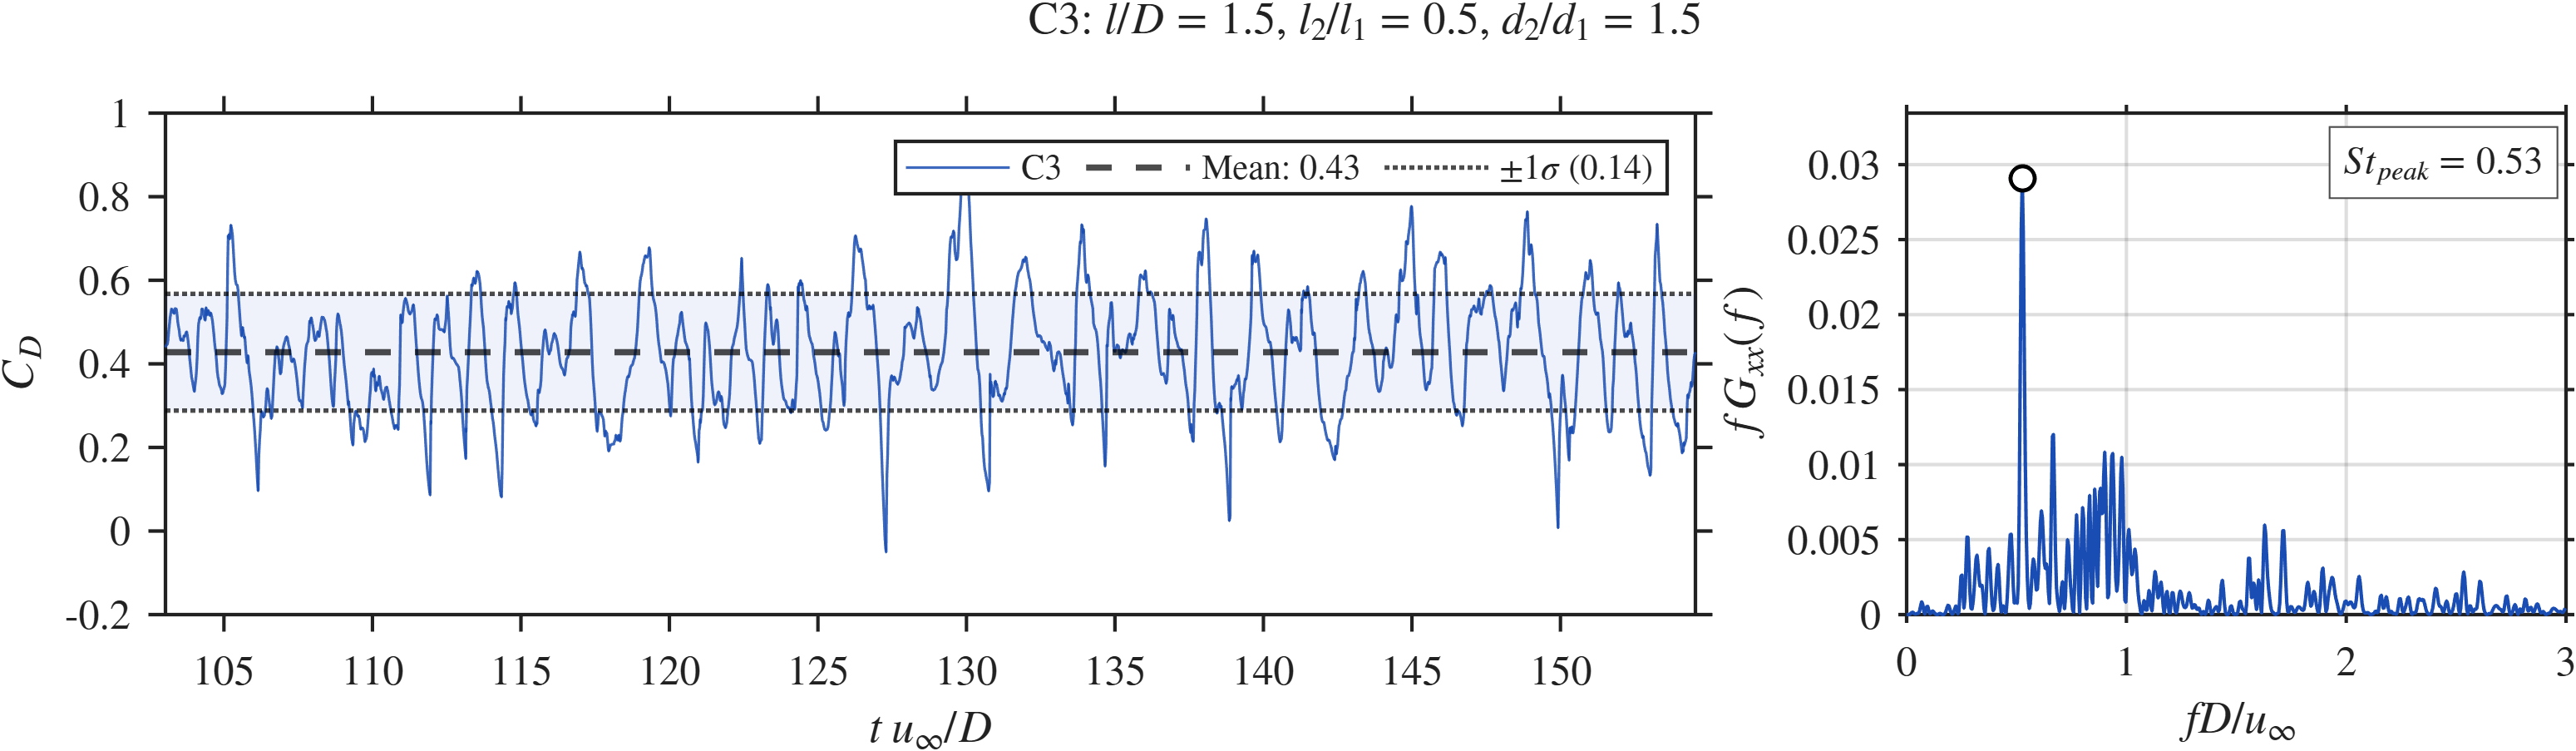
\includegraphics[width=\linewidth]{C3_dsig.png}\caption{C3, drag}\end{subfigure}\\
  \begin{subfigure}{\textwidth}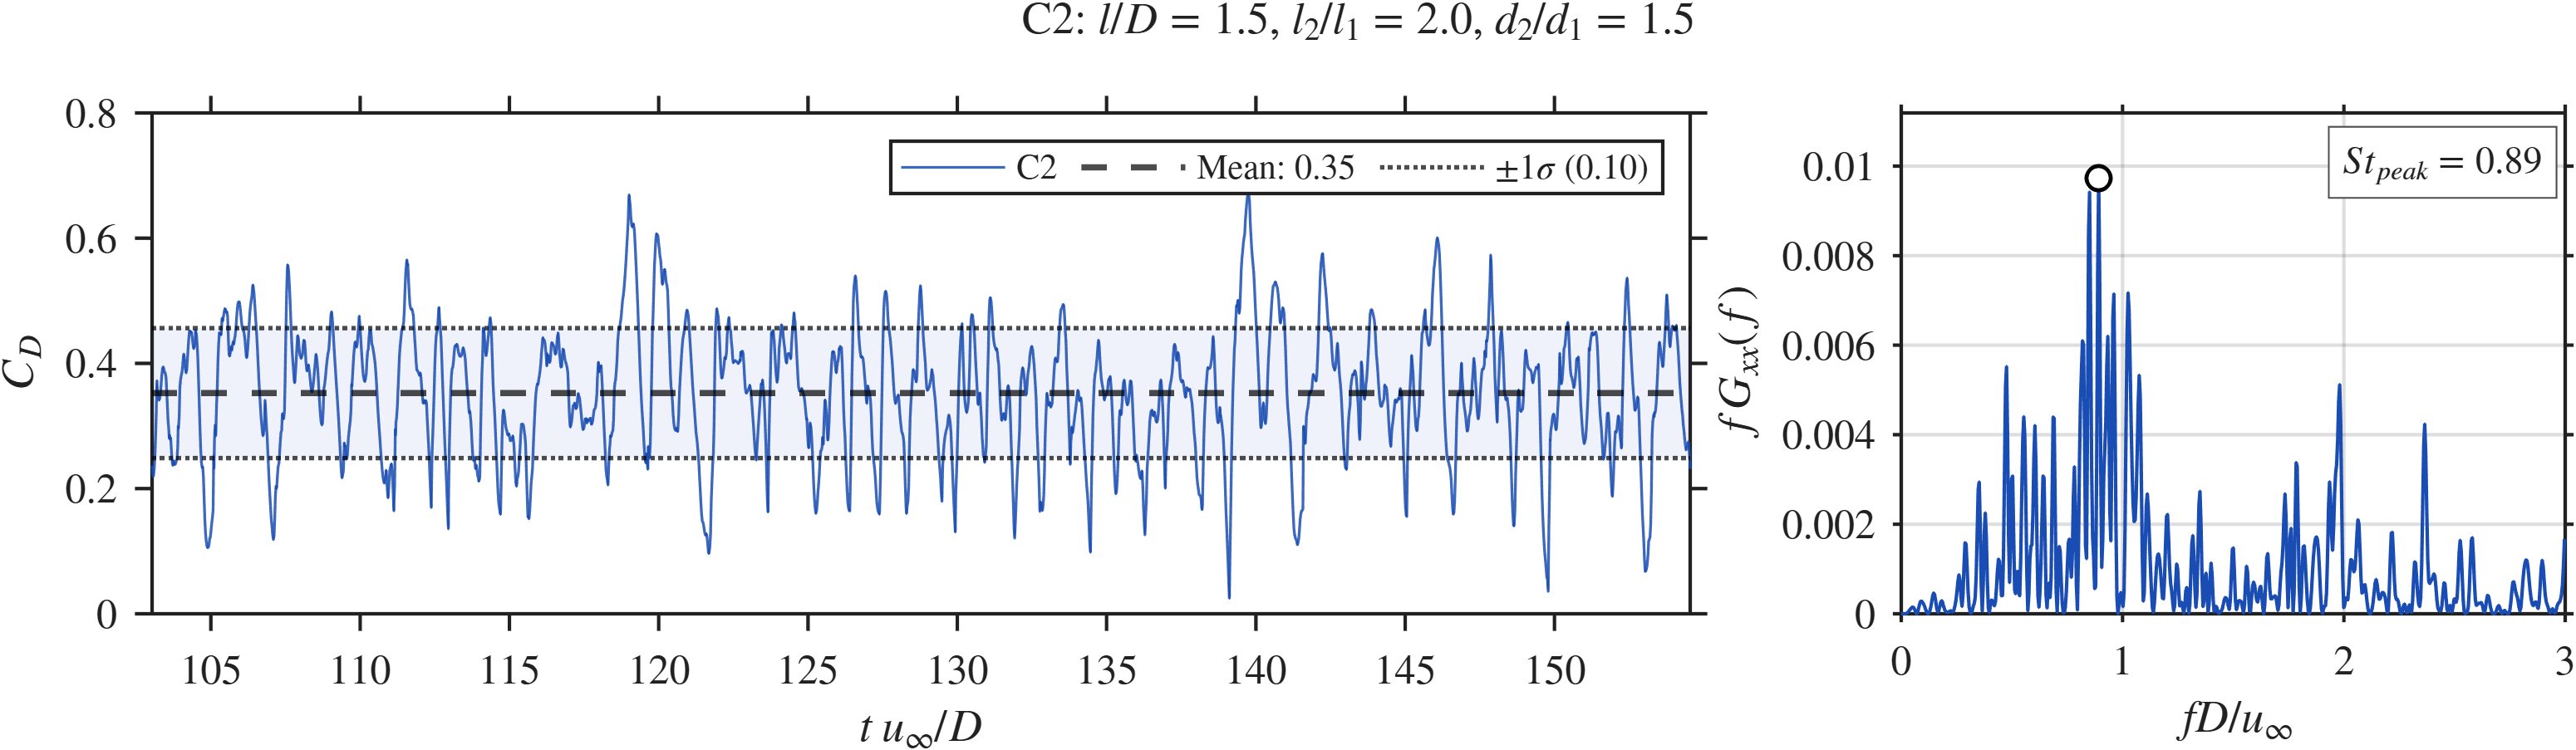
\includegraphics[width=\linewidth]{C2_dsig.png}\caption{C2, drag}\end{subfigure}
  \caption{Gap-ratio sweep: probe pressure and drag signals with spectra for C3 and C2 (C1 is in Fig.~\ref{fig:sac1_sig}).}
  \label{fig:gap_sig}
\end{figure}

\paragraph{SPOD.} Figure~\ref{fig:gap_spod} shows the SPOD results. C3 has the highest peak of this sweep ($\lambda_1 \approx 4\times10^{-5}$ at $St = 0.252$), above the SA peak. Its leading mode has large structures that span both cavities and the hemisphere, a cavity-wide oscillation. The second peak at $St = 0.505$ is twice the first, which points to a strongly non-sinusoidal, pulsation-like cycle. The third peak at $St = 0.893$ has finer structures in Cavity 2 and matches the Cavity 2 band of the $x$--$f$ diagram. C2 has the lowest peak of the sweep ($\lambda_1 \approx 8\times10^{-6}$ at $St = 0.524$), about five times below C3. Its leading mode sits mostly in Cavity 2 and barely enters the short Cavity 1, so the coupling between the cavities is weak. Its other peaks at $St = 1.106$ and 1.728 show finer shear-layer structures.

\begin{figure}[htbp]
  \centering
  \begin{subfigure}{0.72\textwidth}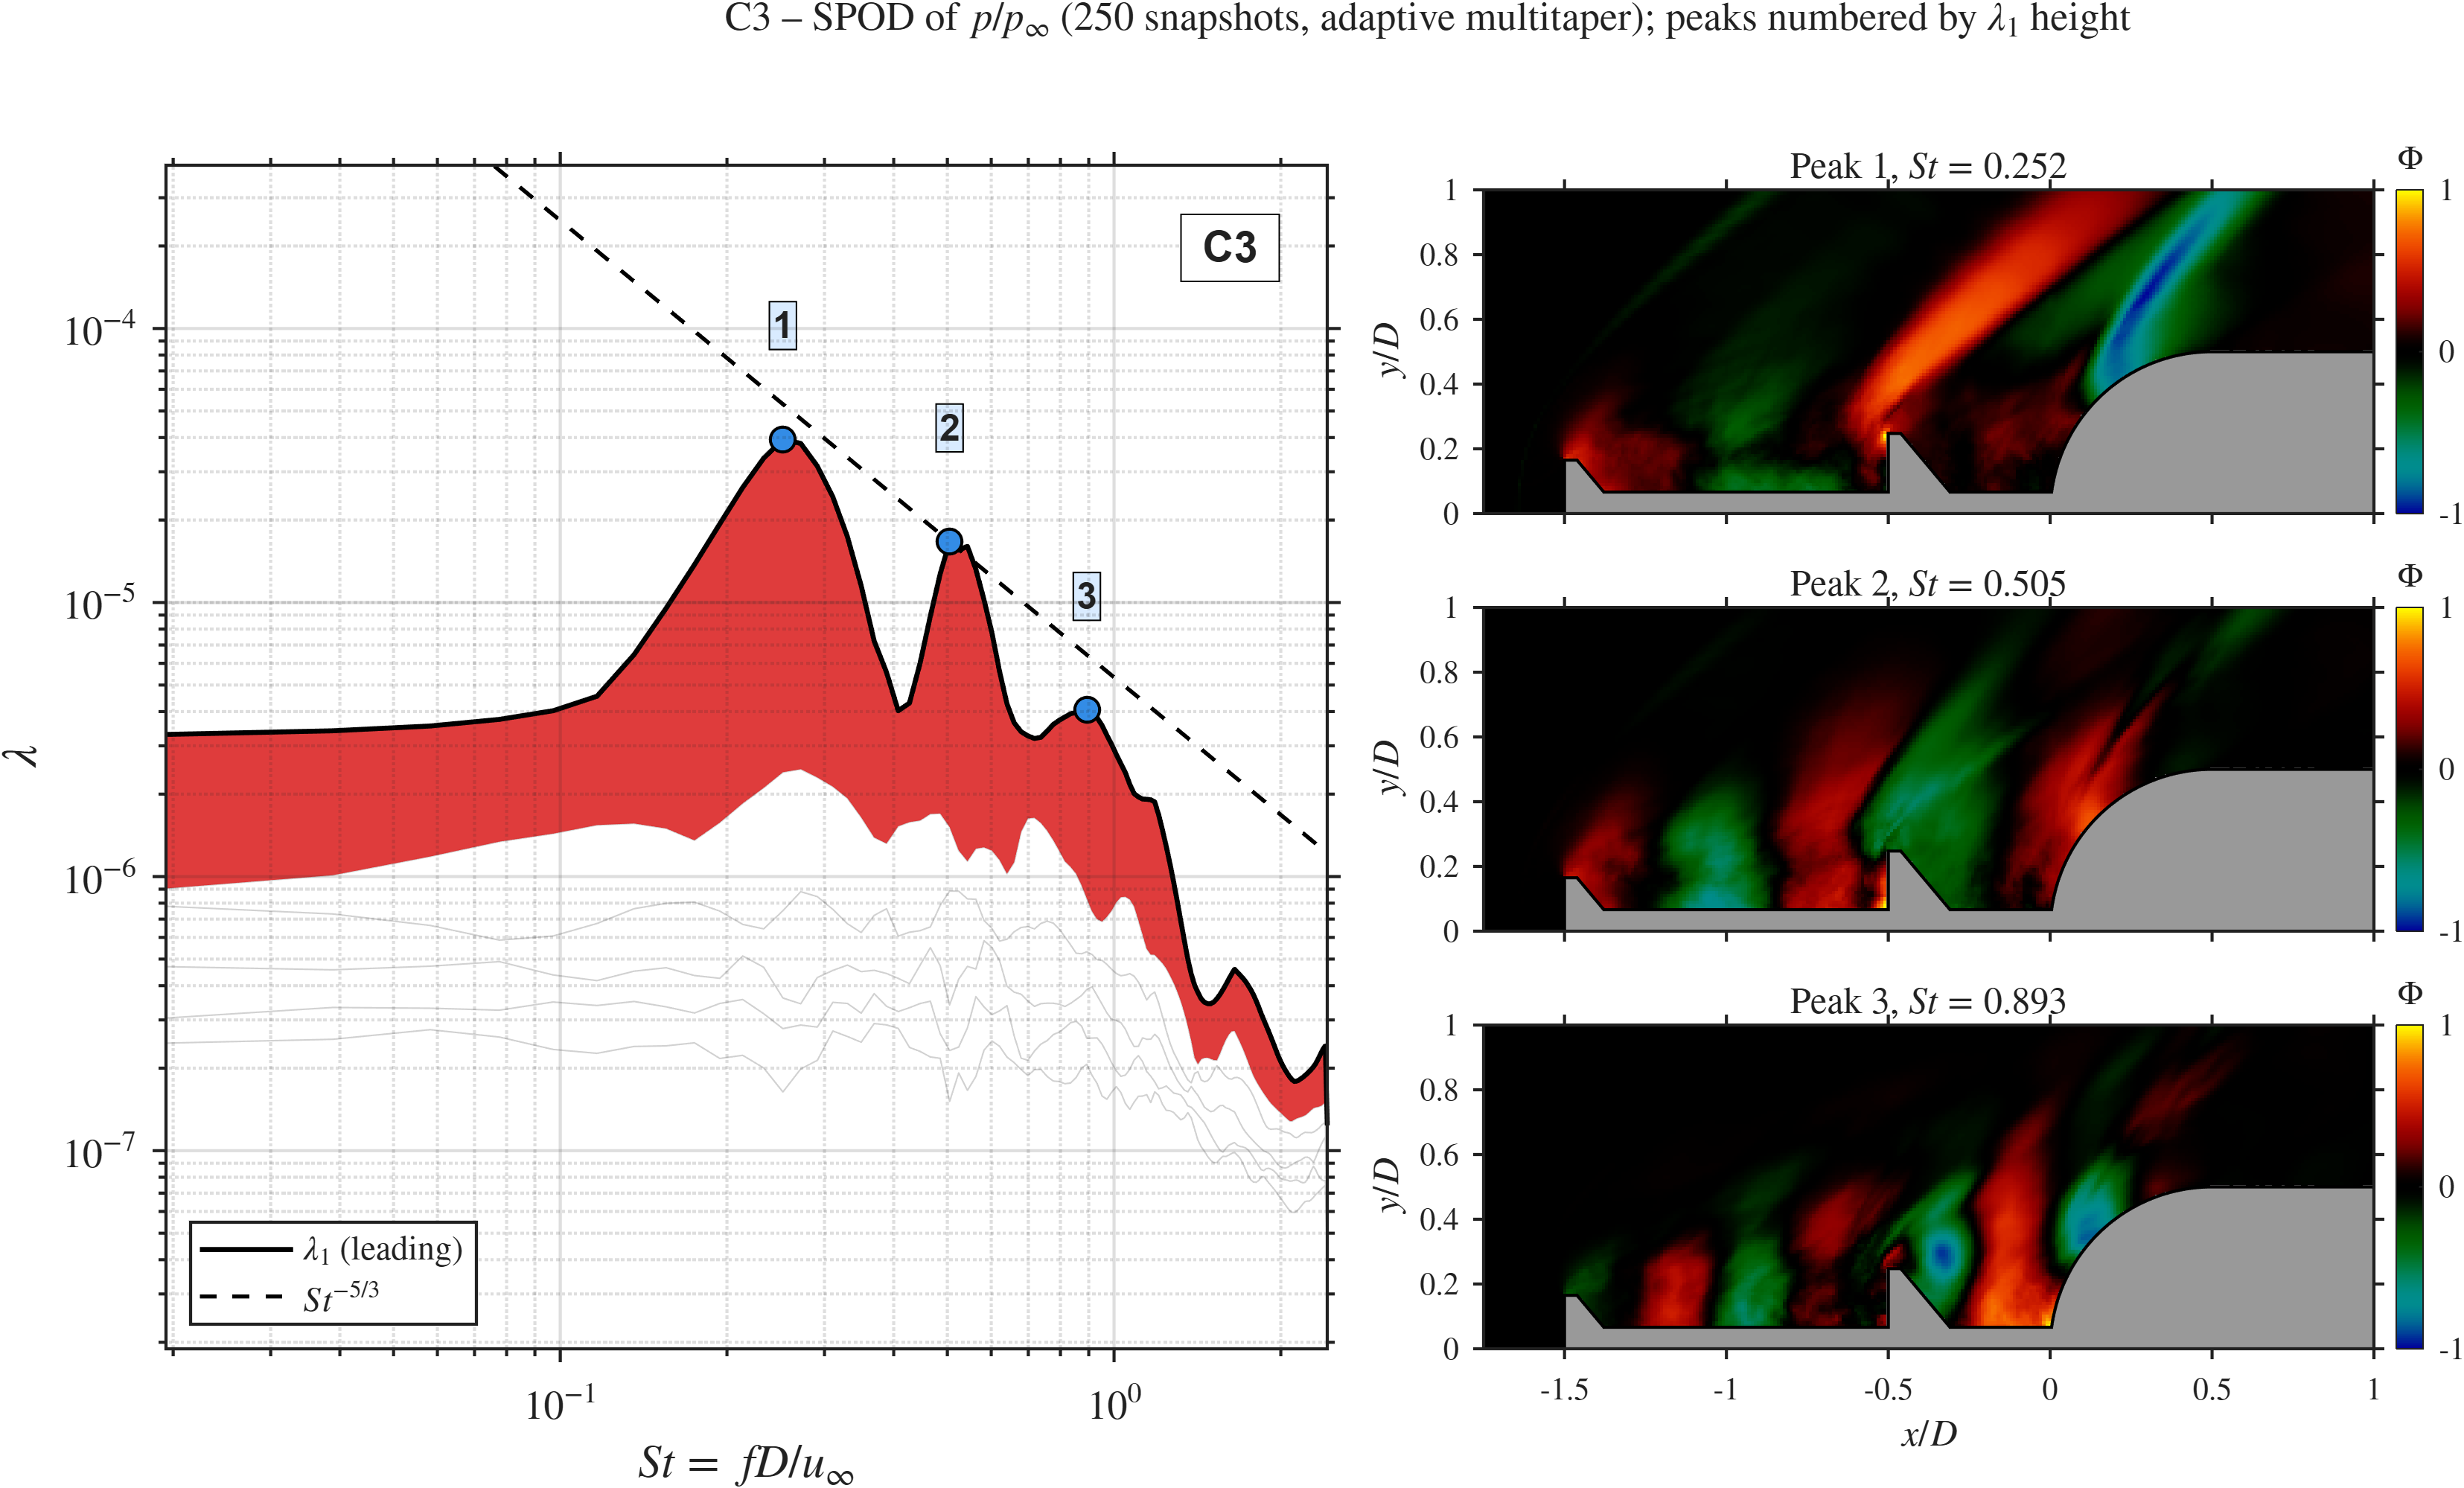
\includegraphics[width=\linewidth]{C3_spod.png}\caption{C3 ($\ltl = 0.5$)}\end{subfigure}\\
  \begin{subfigure}{0.72\textwidth}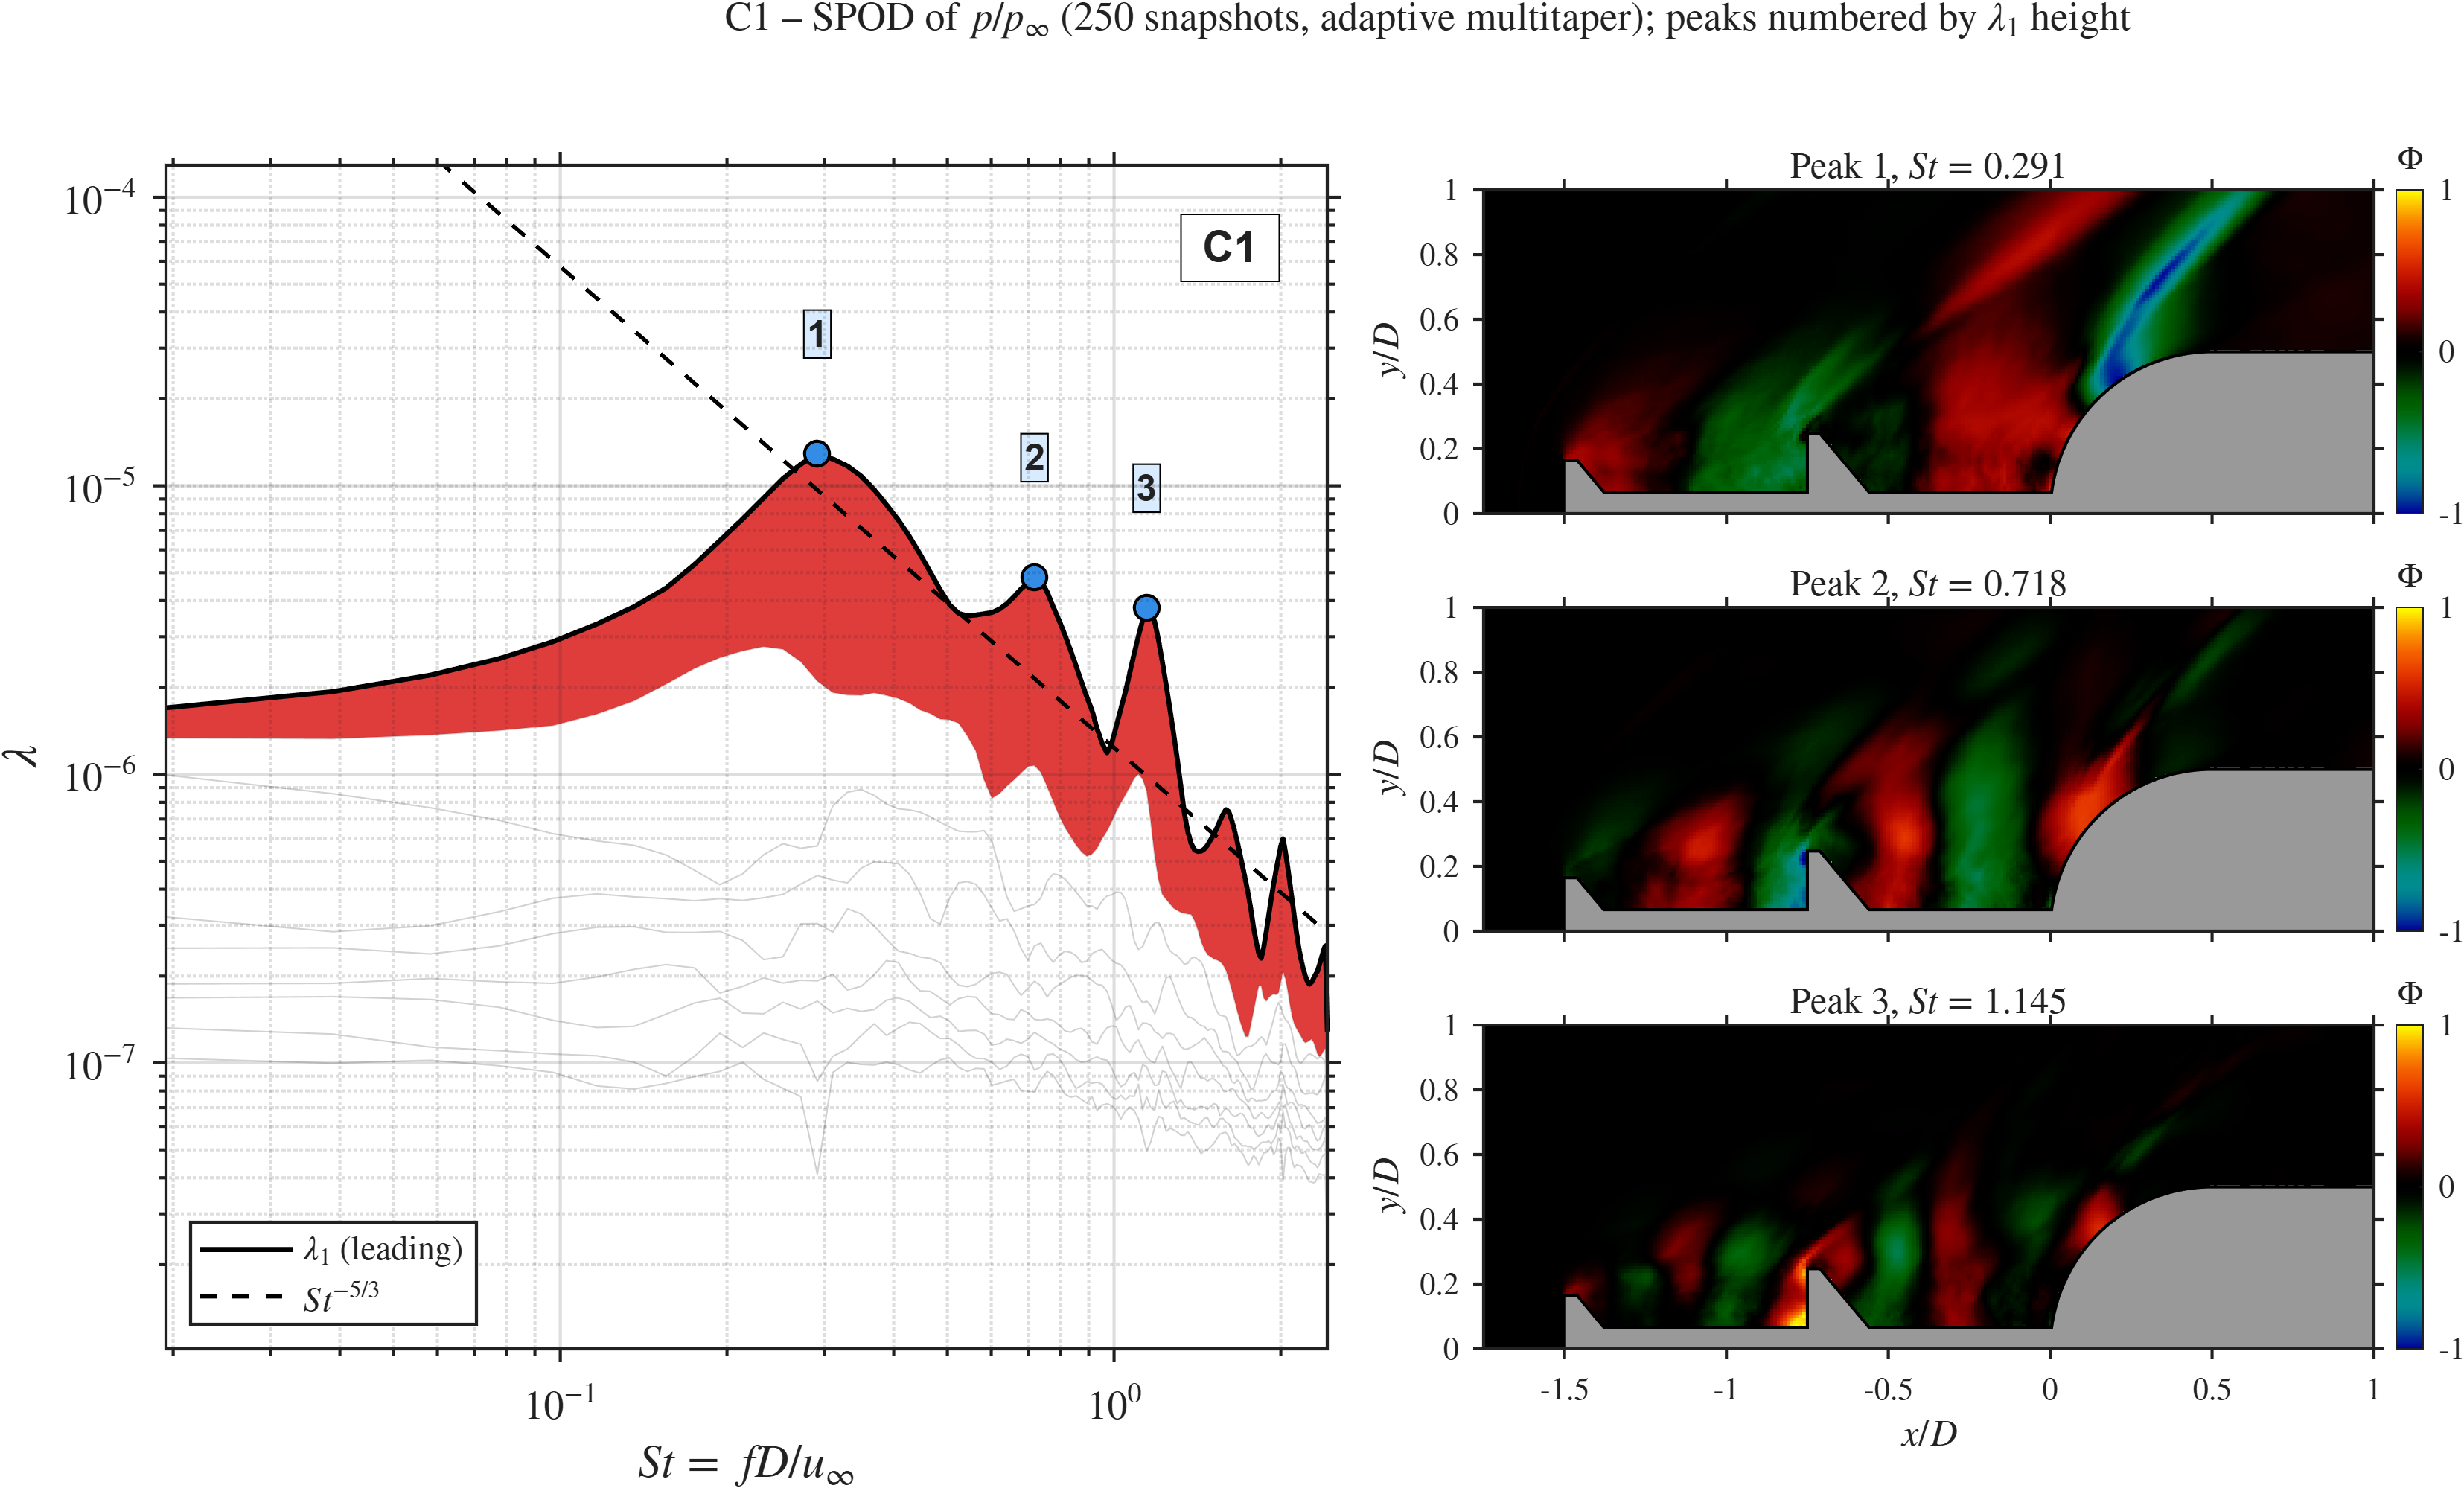
\includegraphics[width=\linewidth]{C1_spod.png}\caption{C1 ($\ltl = 1$)}\end{subfigure}\\
  \begin{subfigure}{0.72\textwidth}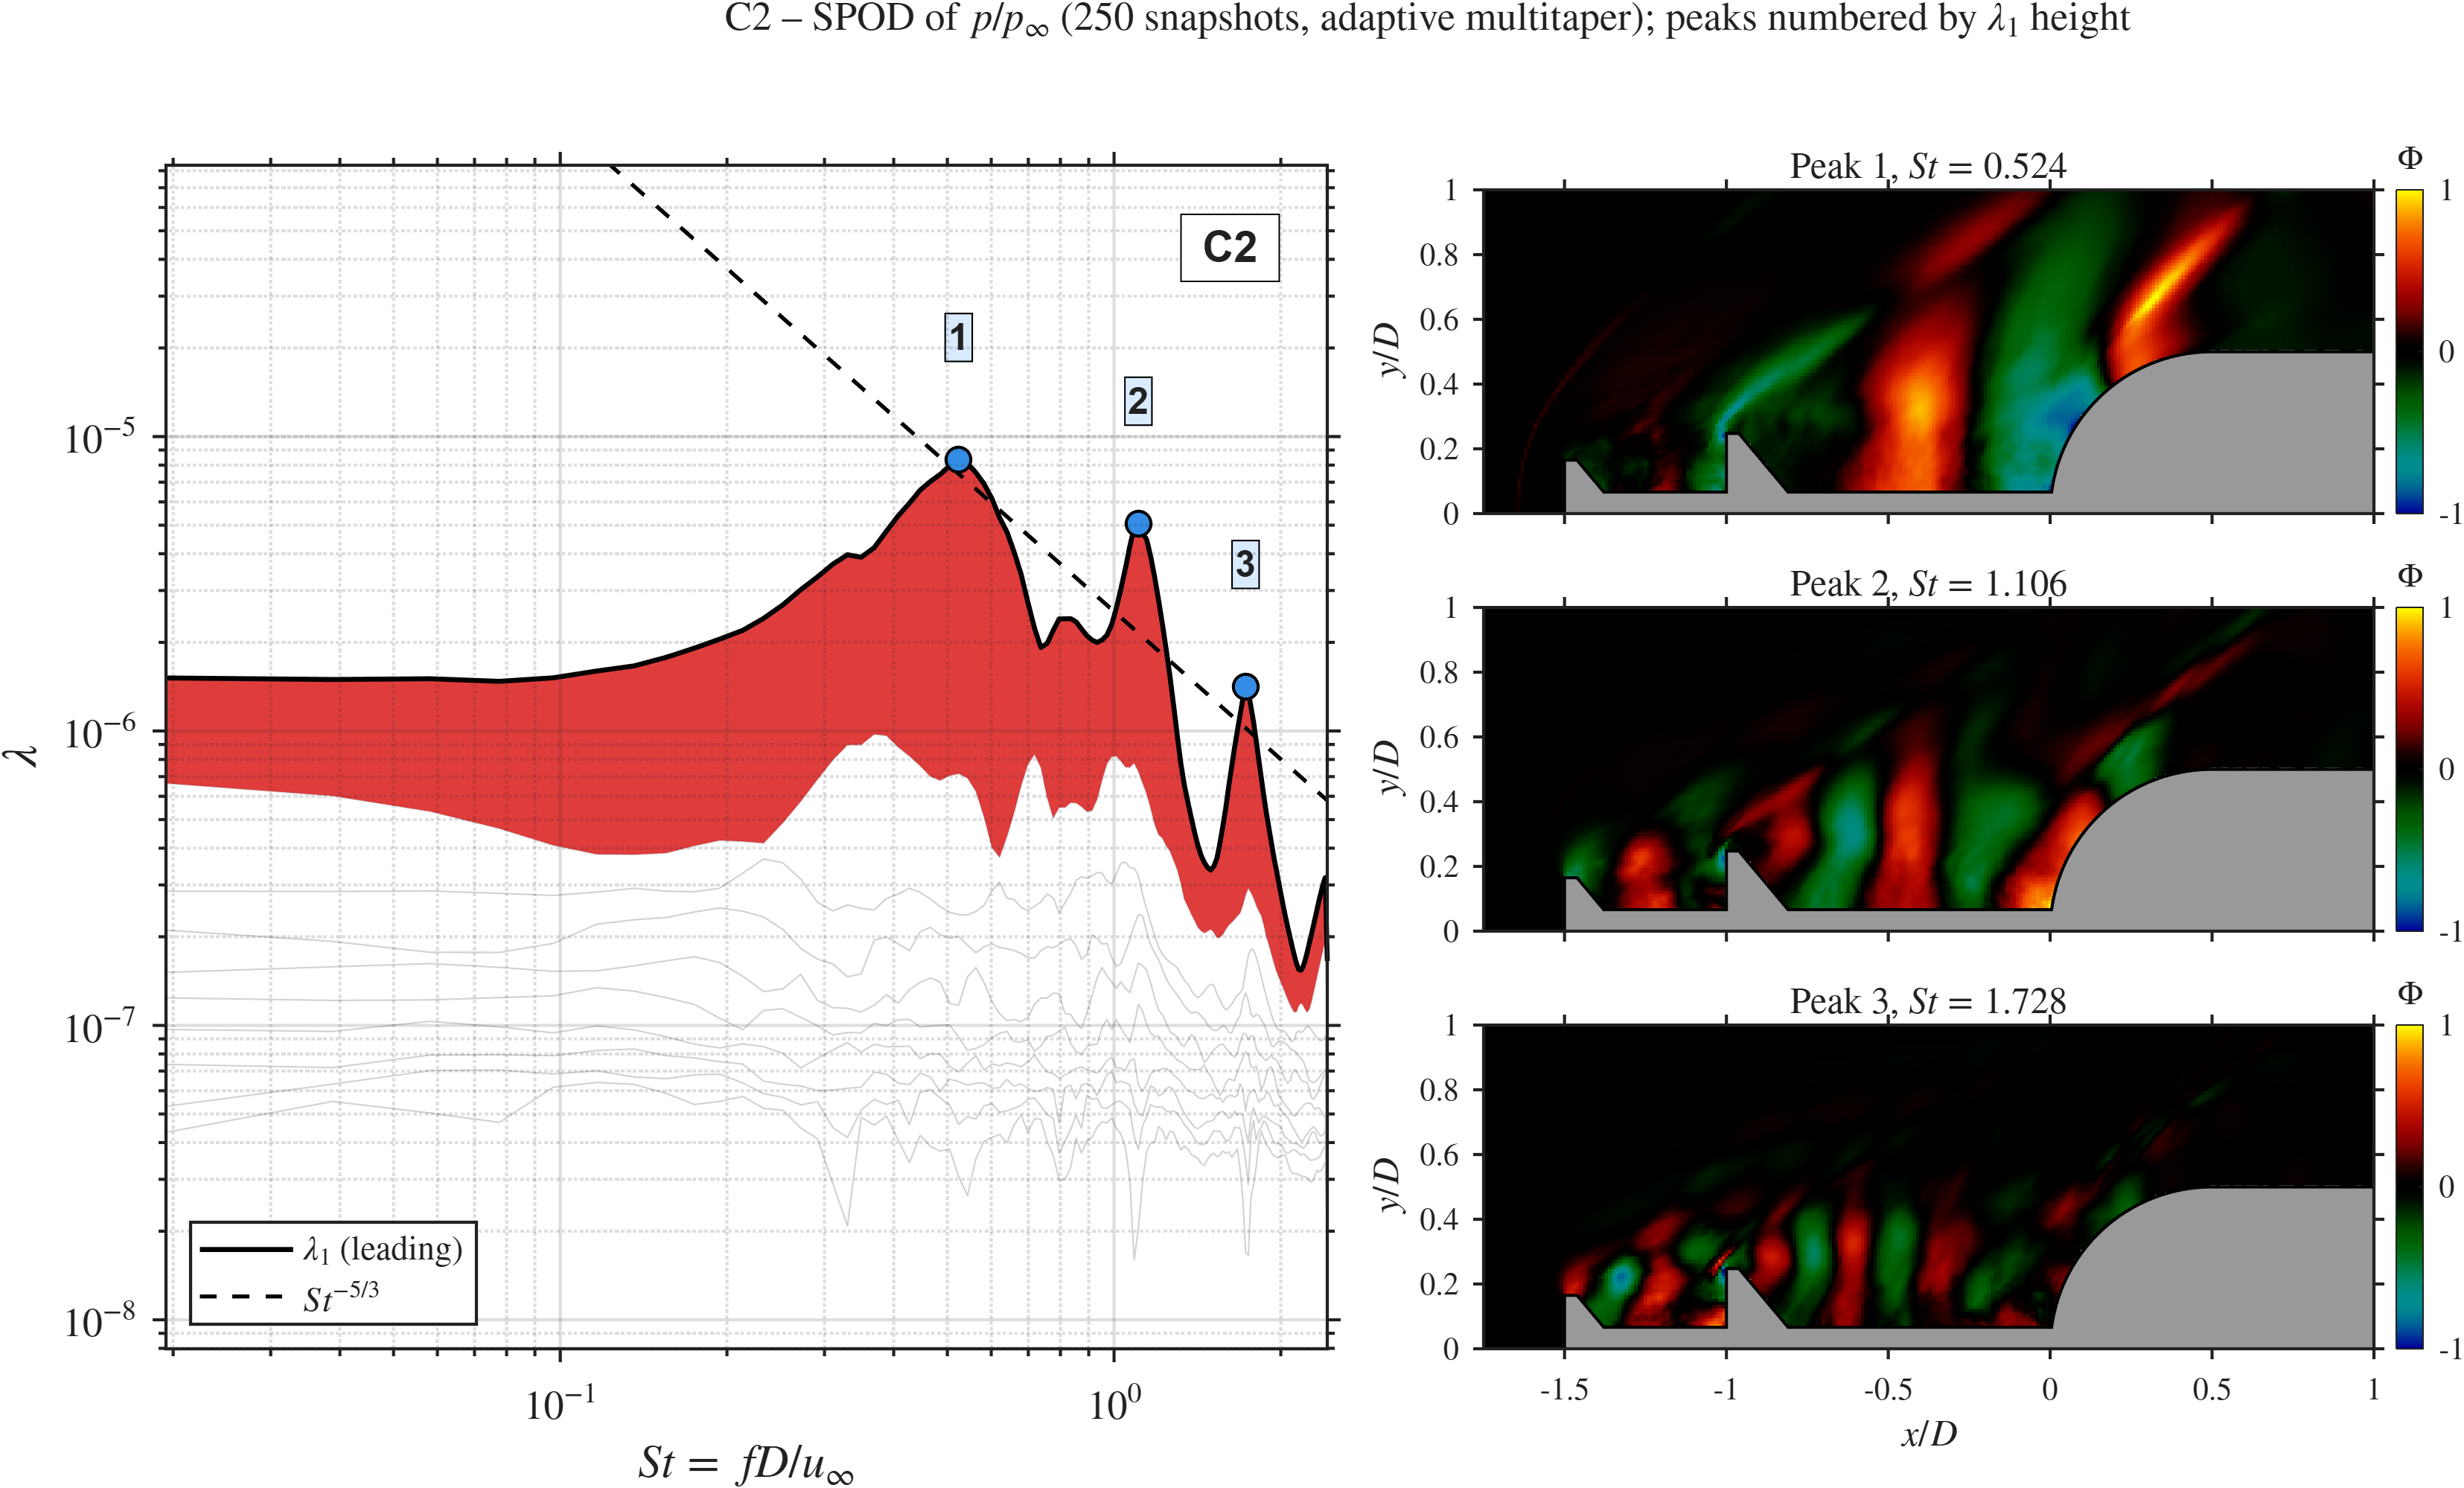
\includegraphics[width=\linewidth]{C2_spod.png}\caption{C2 ($\ltl = 2$)}\end{subfigure}
  \caption{Gap-ratio sweep: SPOD spectra and leading modes.}
  \label{fig:gap_spod}
\end{figure}

\paragraph{Summary.} Table~\ref{tab:gap} lists the trends. Moving the second disk forward (larger $\ltl$) lowers the shoulder pressure, the fluctuation level, the mean drag and the drag fluctuation together. $\Cdm$ falls by 18.6\%, from 0.43 (C3) to 0.35 (C2), and $\lambda_1$ falls about fivefold. C2 has the lowest mean drag of all eight cases, 2.8\% below SA, with the same drag fluctuation as SA and a tonal peak about 86\% lower. This fits our steady RANS result that a forward-placed second disk ($\ltl = 2$) traps a compressed vortex that acts as a pneumatic buffer~\cite{Gujar2026staged}. A short Cavity 2 ($\ltl = 0.5$) gives a low-frequency, pulsation-like mode with strong coherent energy. A long Cavity 2 ($\ltl = 2$) weakens the coupling between the cavities and the flow moves back toward SA-like behaviour.

\begin{table}[htbp]
  \centering
  \caption{Gap-ratio sweep. Percentages are relative to the pivot C1.}
  \label{tab:gap}
  \begin{tabular}{lcccl}
    \toprule
    Metric & C3 ($\ltl = 0.5$) & C1 ($\ltl = 1$) & C2 ($\ltl = 2$) & Trend with $\ltl$ \\
    \midrule
    $\pbar$ & 1.98 ($+6.5\%$) & 1.86 & 1.67 ($-10.2\%$) & falls \\
    $\psd$ & 0.76 ($+4.1\%$) & 0.73 & 0.68 ($-6.8\%$) & falls \\
    $\Cdm$ & 0.43 ($+10.3\%$) & 0.39 & 0.35 ($-10.3\%$) & falls \\
    $\sCd$ & 0.14 ($+16.7\%$) & 0.12 & 0.10 ($-16.7\%$) & falls \\
    $St$ peak, pressure & 0.25 & 1.12 & 0.56 & non-monotonic \\
    $St$ peak, drag & 0.53 & 1.14 & 0.89 & non-monotonic \\
    Peak $\Pi$ & $\approx 0.61$ & $\approx 0.37$ & $\approx 0.50$ & non-monotonic \\
    SPOD leading $St$ & 0.252 & 0.291 & 0.524 & rises \\
    SPOD peak $\lambda_1$ & $\approx 4\times10^{-5}$ & $\approx 1.3\times10^{-5}$ & $\approx 8\times10^{-6}$ & falls \\
    \bottomrule
  \end{tabular}
\end{table}

% ------------------------------------------------------------
\subsection{Effect of the disk diameter ratio $\dtd$ (C4, C1, C5)}\label{sec:dia}

This sweep changes the diameter of the second disk at fixed $l/D = 1.5$ and $\ltl = 1$, so both cavities are $0.75D$ long (RQ2). The second-disk radius is $0.165D$ in C4 (equal to the primary disk), $0.248D$ in C1 and $0.330D$ in C5.

\paragraph{Mean flow and fluctuations.} Figure~\ref{fig:dia_ms} shows the contours. C4 ($\dtd = 1$) has the highest shoulder pressure of all cases ($\pbar = 2.12$). A second disk of the same size as the primary does not widen the effective body. The shear layer from the primary disk passes over its edge with little deflection, so the second disk takes little energy out of the separated flow, and the shear layer reaches Cavity 2 and the shoulder almost unchanged. The streamlines show one large recirculation spanning both cavities, so the equal disk does not split the dead-air zone. C5 ($\dtd = 2$) is the other extreme. Its second disk reaches 66\% of the hemisphere radius, intercepts the Cavity 1 shear layer and turns it outward through an expansion fan at the disk edge. The shoulder pressure drops to $\pbar = 1.45$, the lowest of all cases and 18.5\% below SA. Each cavity holds its own recirculation cell. In the fluctuation fields, C4 has the widest band of $\psd > 0.4$, running from the primary disk through Cavity 2 to the shoulder. C5 has lower fluctuations at the shoulder, but its second-disk face and edge become a strong source of their own ($\psd > 0.8$).

\begin{figure}[htbp]
  \centering
  \begin{subfigure}{0.49\textwidth}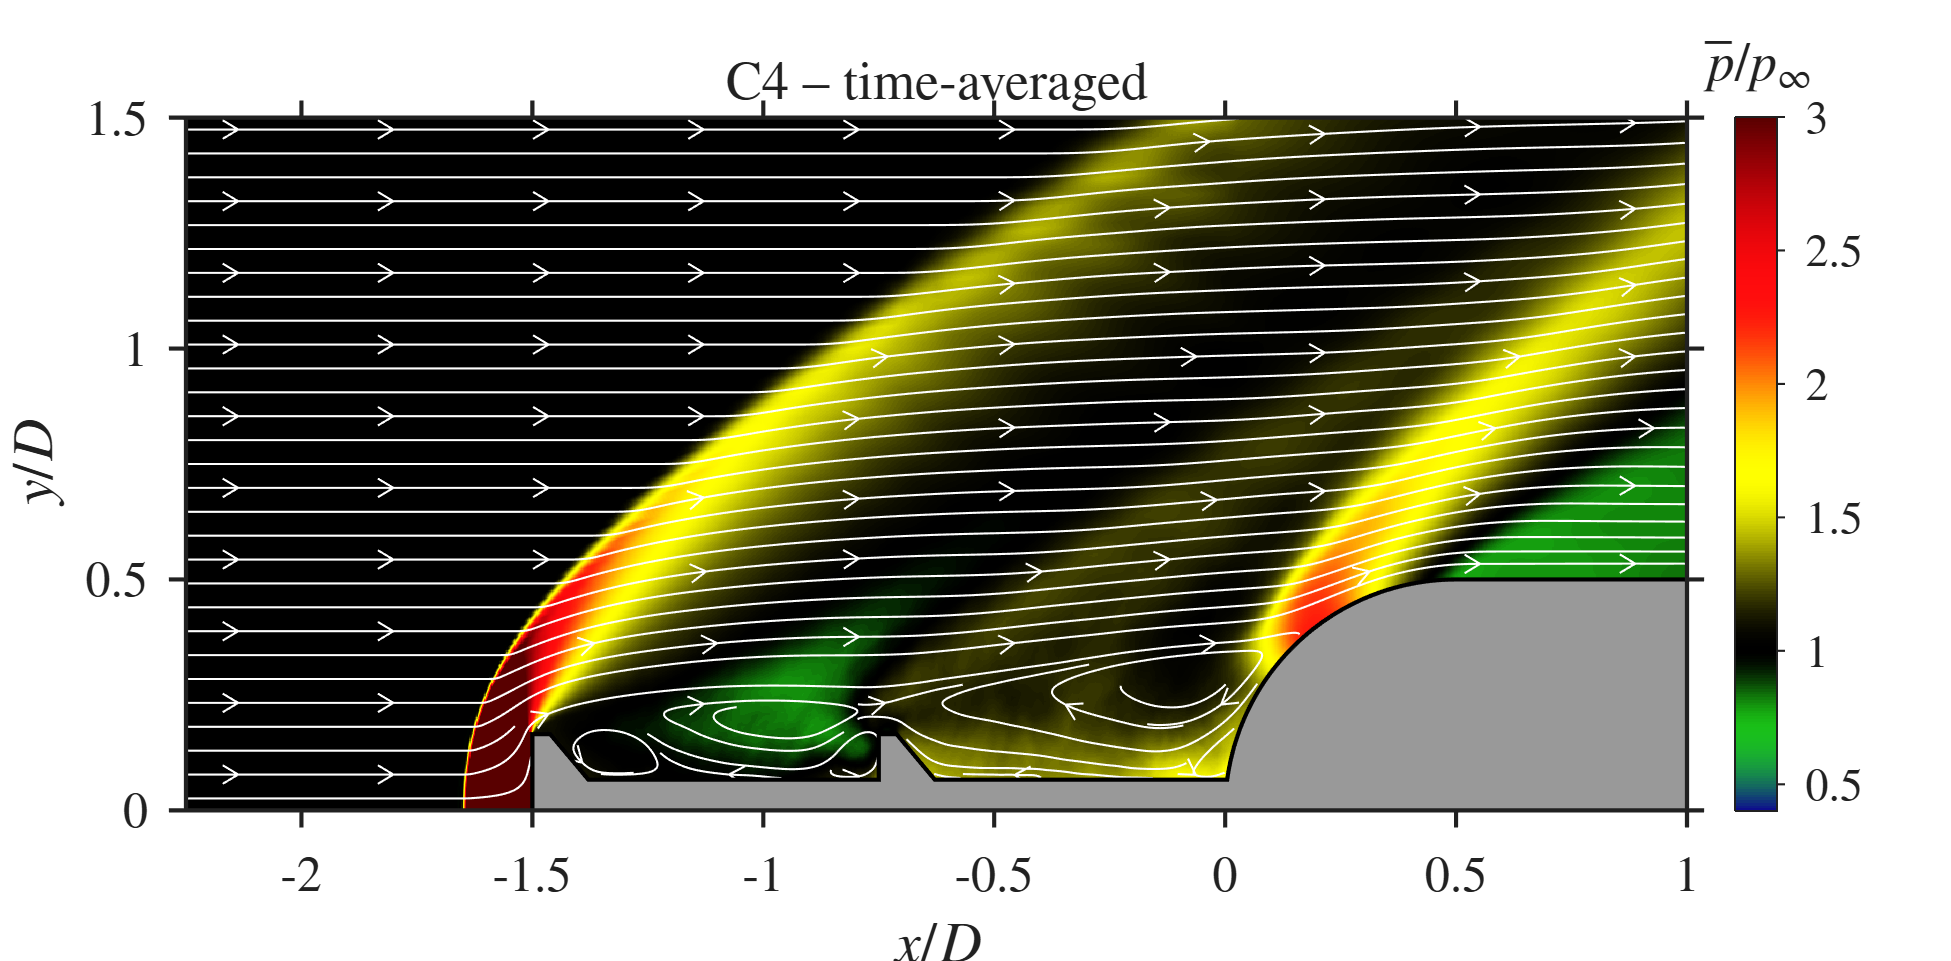
\includegraphics[width=\linewidth]{C4_mean.png}\caption{C4 ($\dtd = 1$), $\pbar$}\end{subfigure}
  \begin{subfigure}{0.49\textwidth}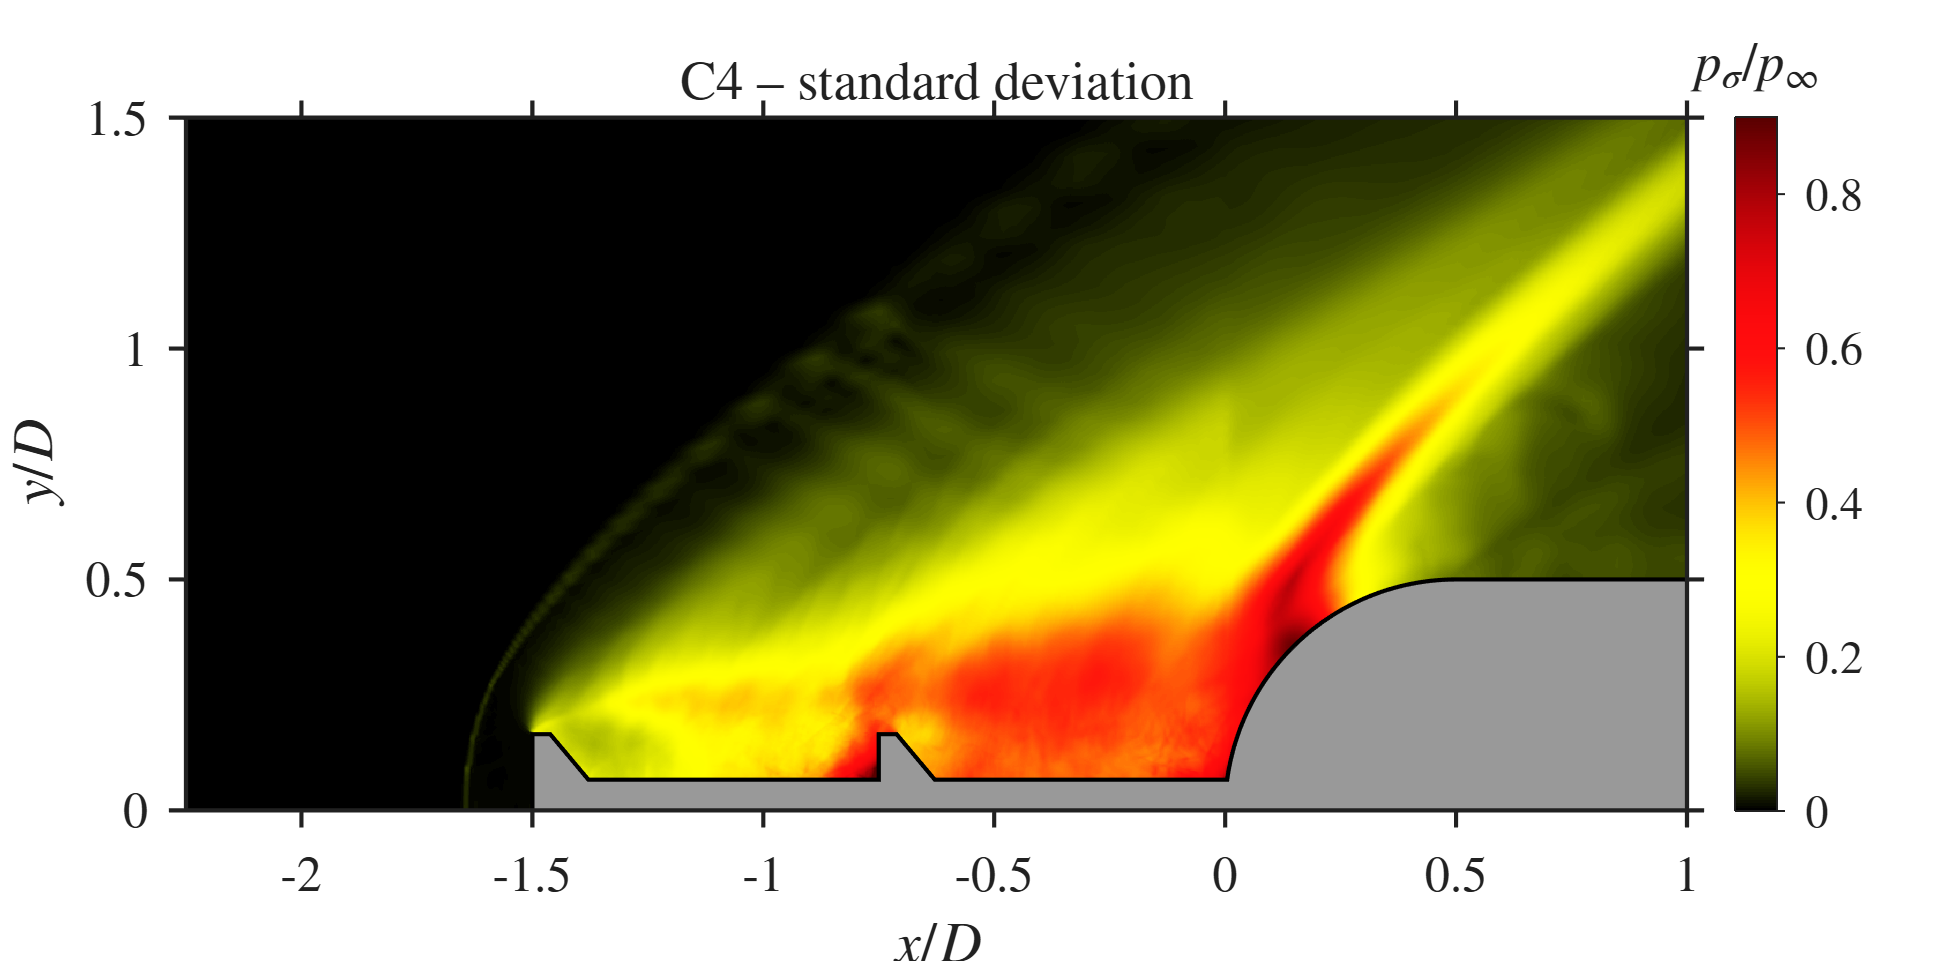
\includegraphics[width=\linewidth]{C4_std.png}\caption{C4, $\psd$}\end{subfigure}\\[2pt]
  \begin{subfigure}{0.49\textwidth}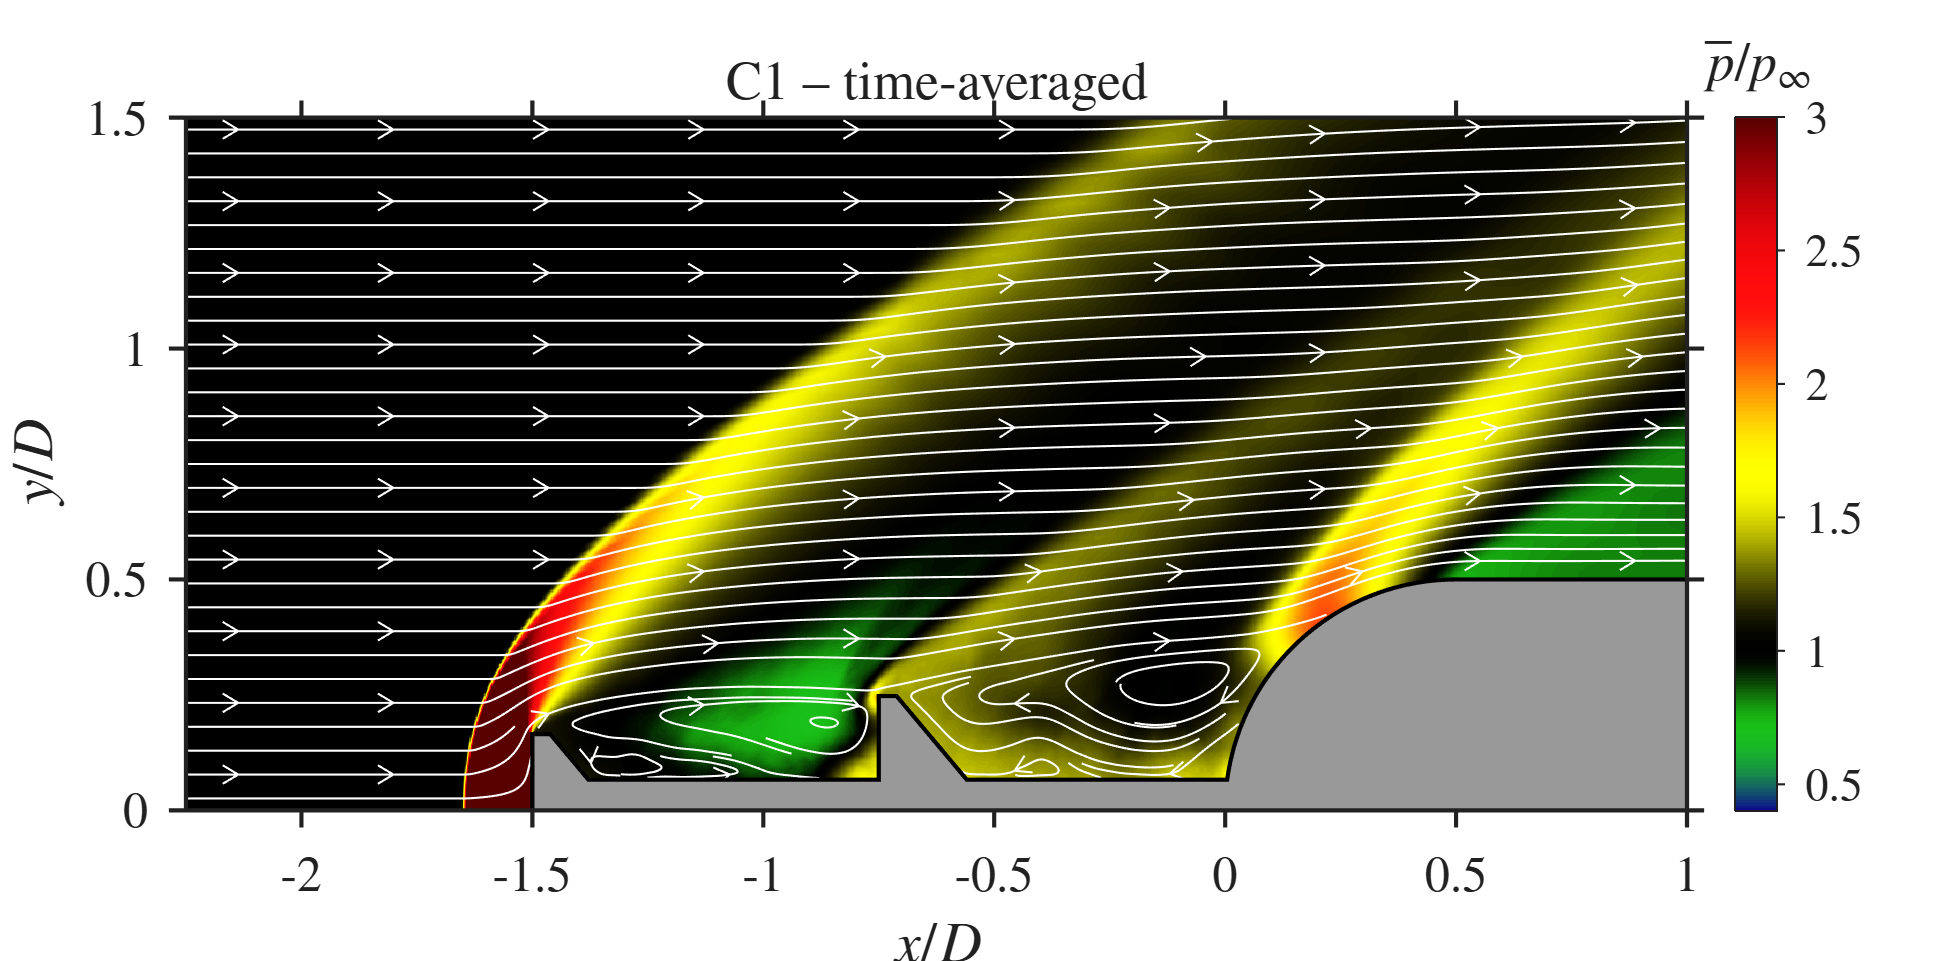
\includegraphics[width=\linewidth]{C1_mean.png}\caption{C1 ($\dtd = 1.5$), $\pbar$}\end{subfigure}
  \begin{subfigure}{0.49\textwidth}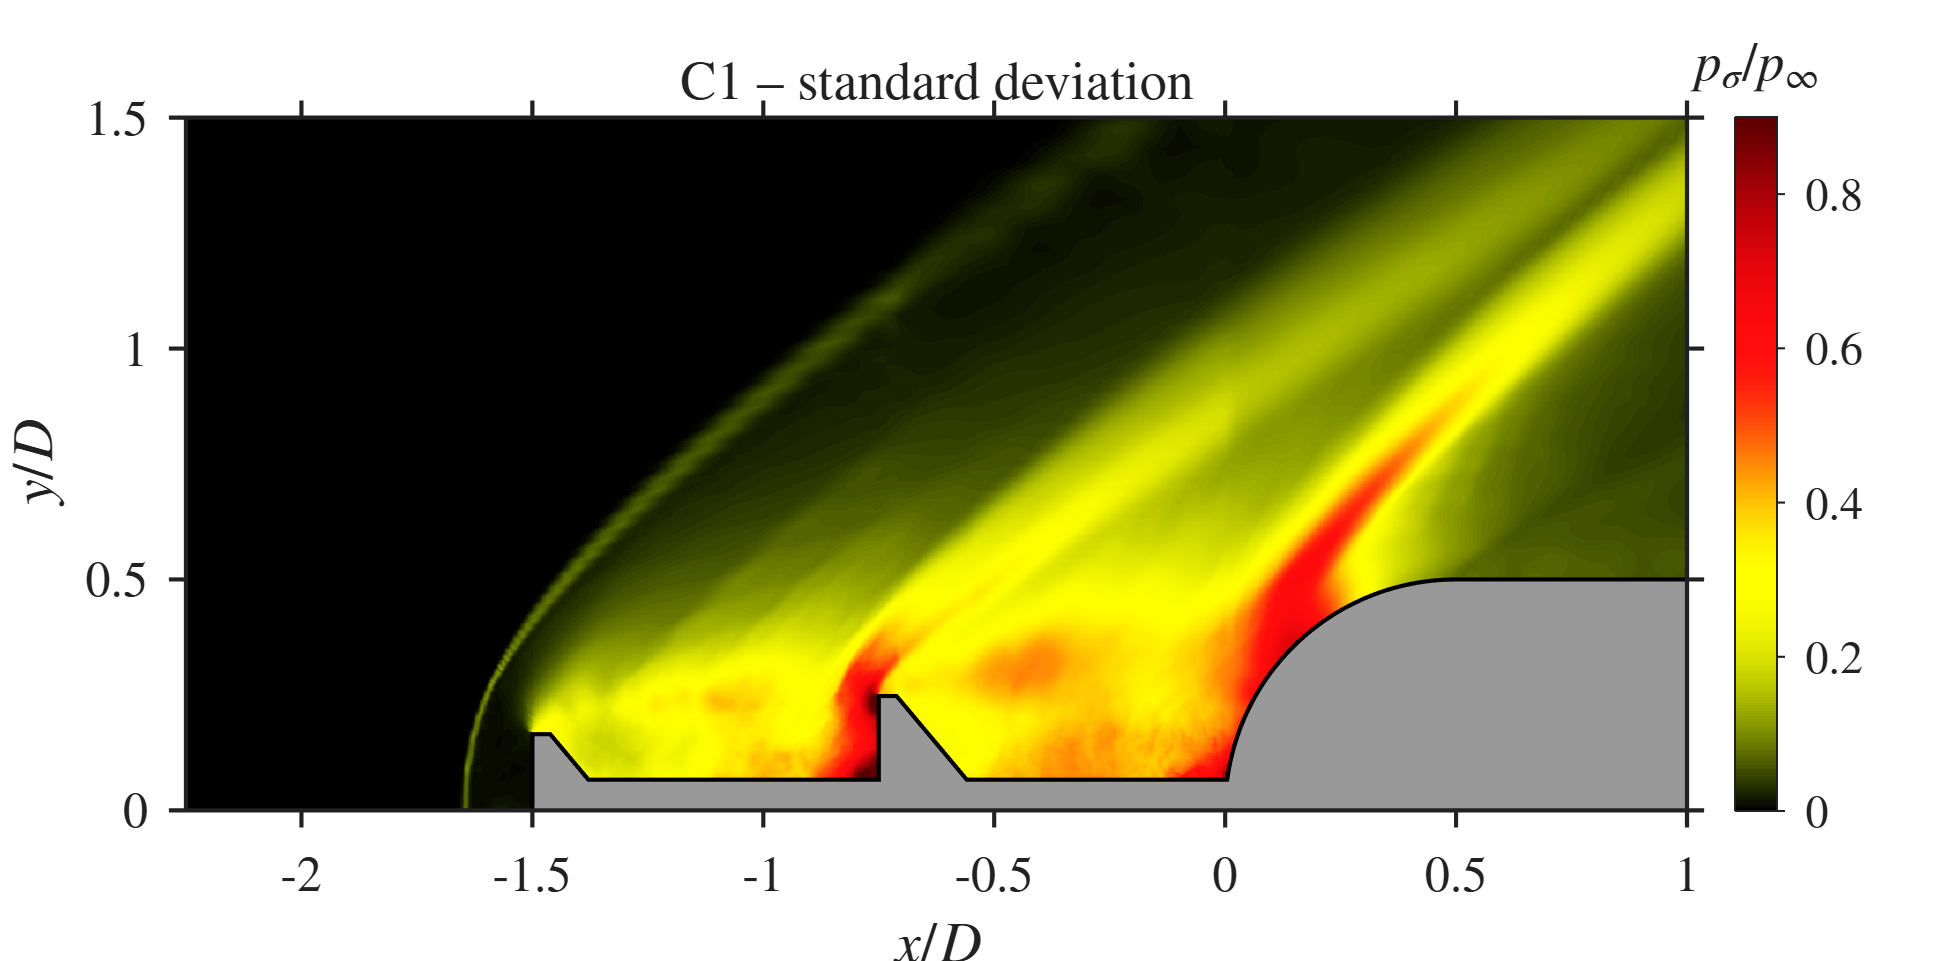
\includegraphics[width=\linewidth]{C1_std.png}\caption{C1, $\psd$}\end{subfigure}\\[2pt]
  \begin{subfigure}{0.49\textwidth}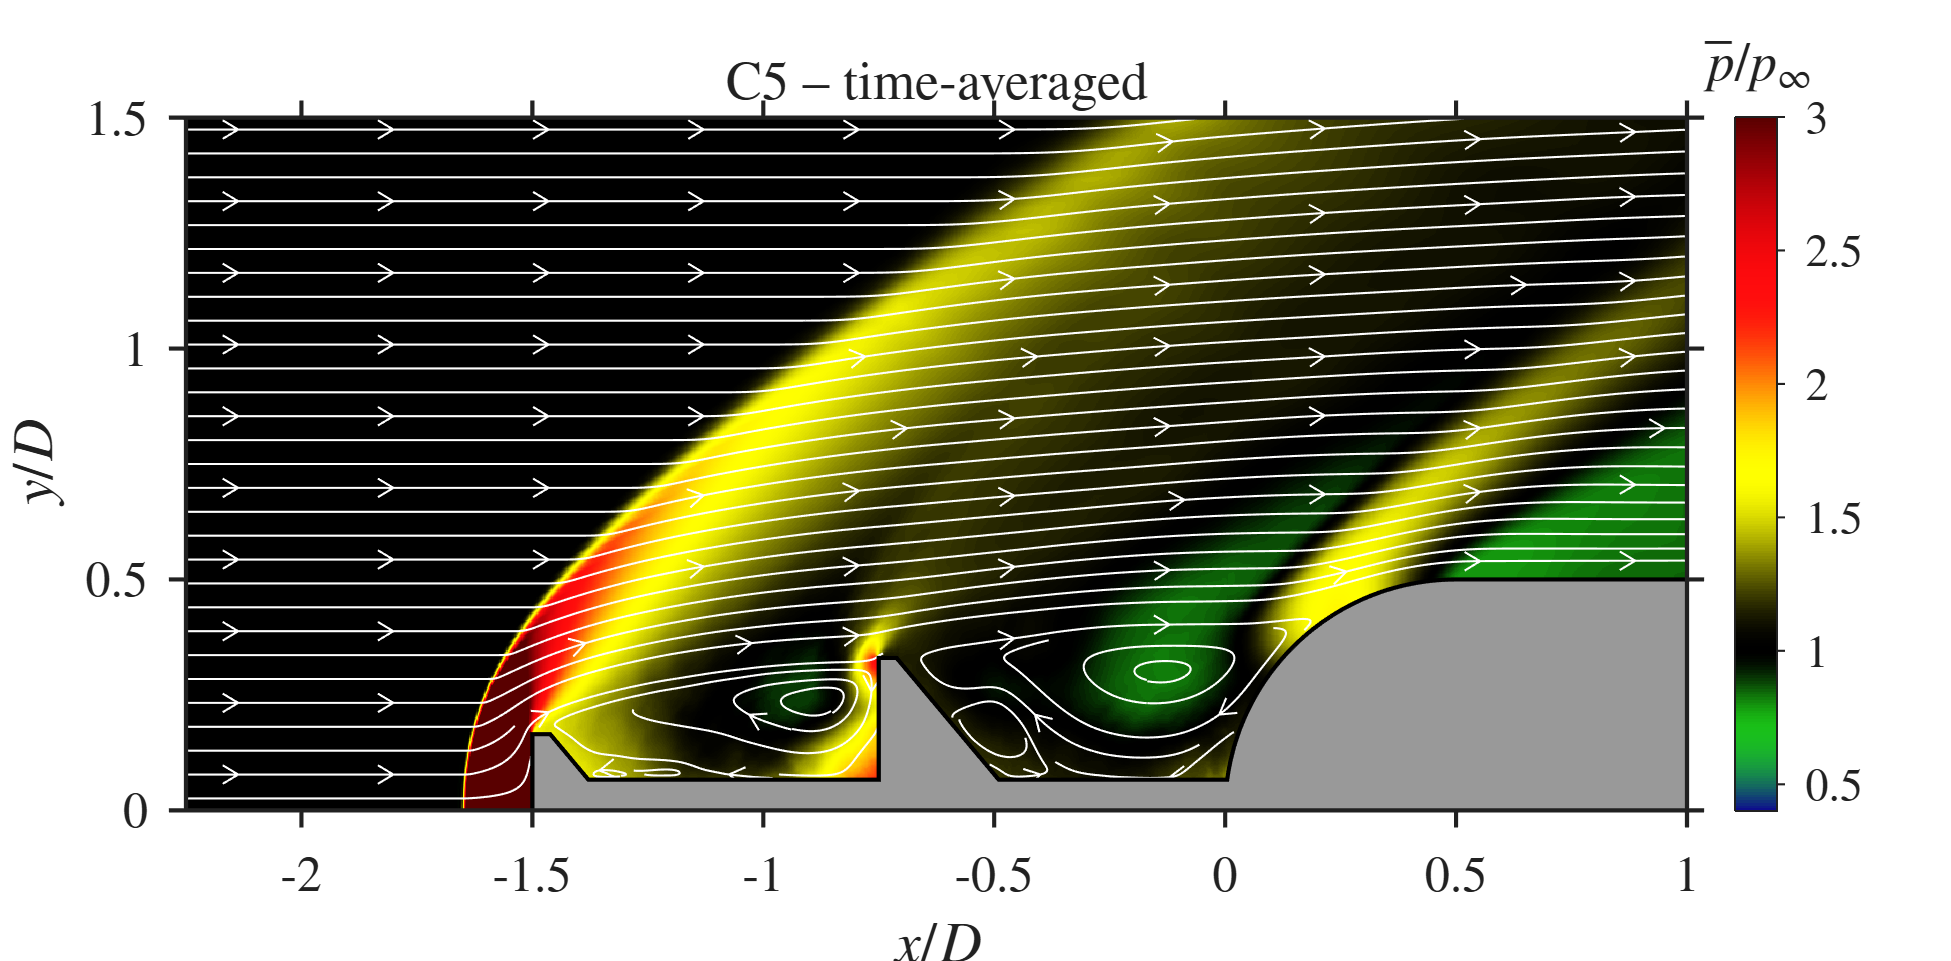
\includegraphics[width=\linewidth]{C5_mean.png}\caption{C5 ($\dtd = 2$), $\pbar$}\end{subfigure}
  \begin{subfigure}{0.49\textwidth}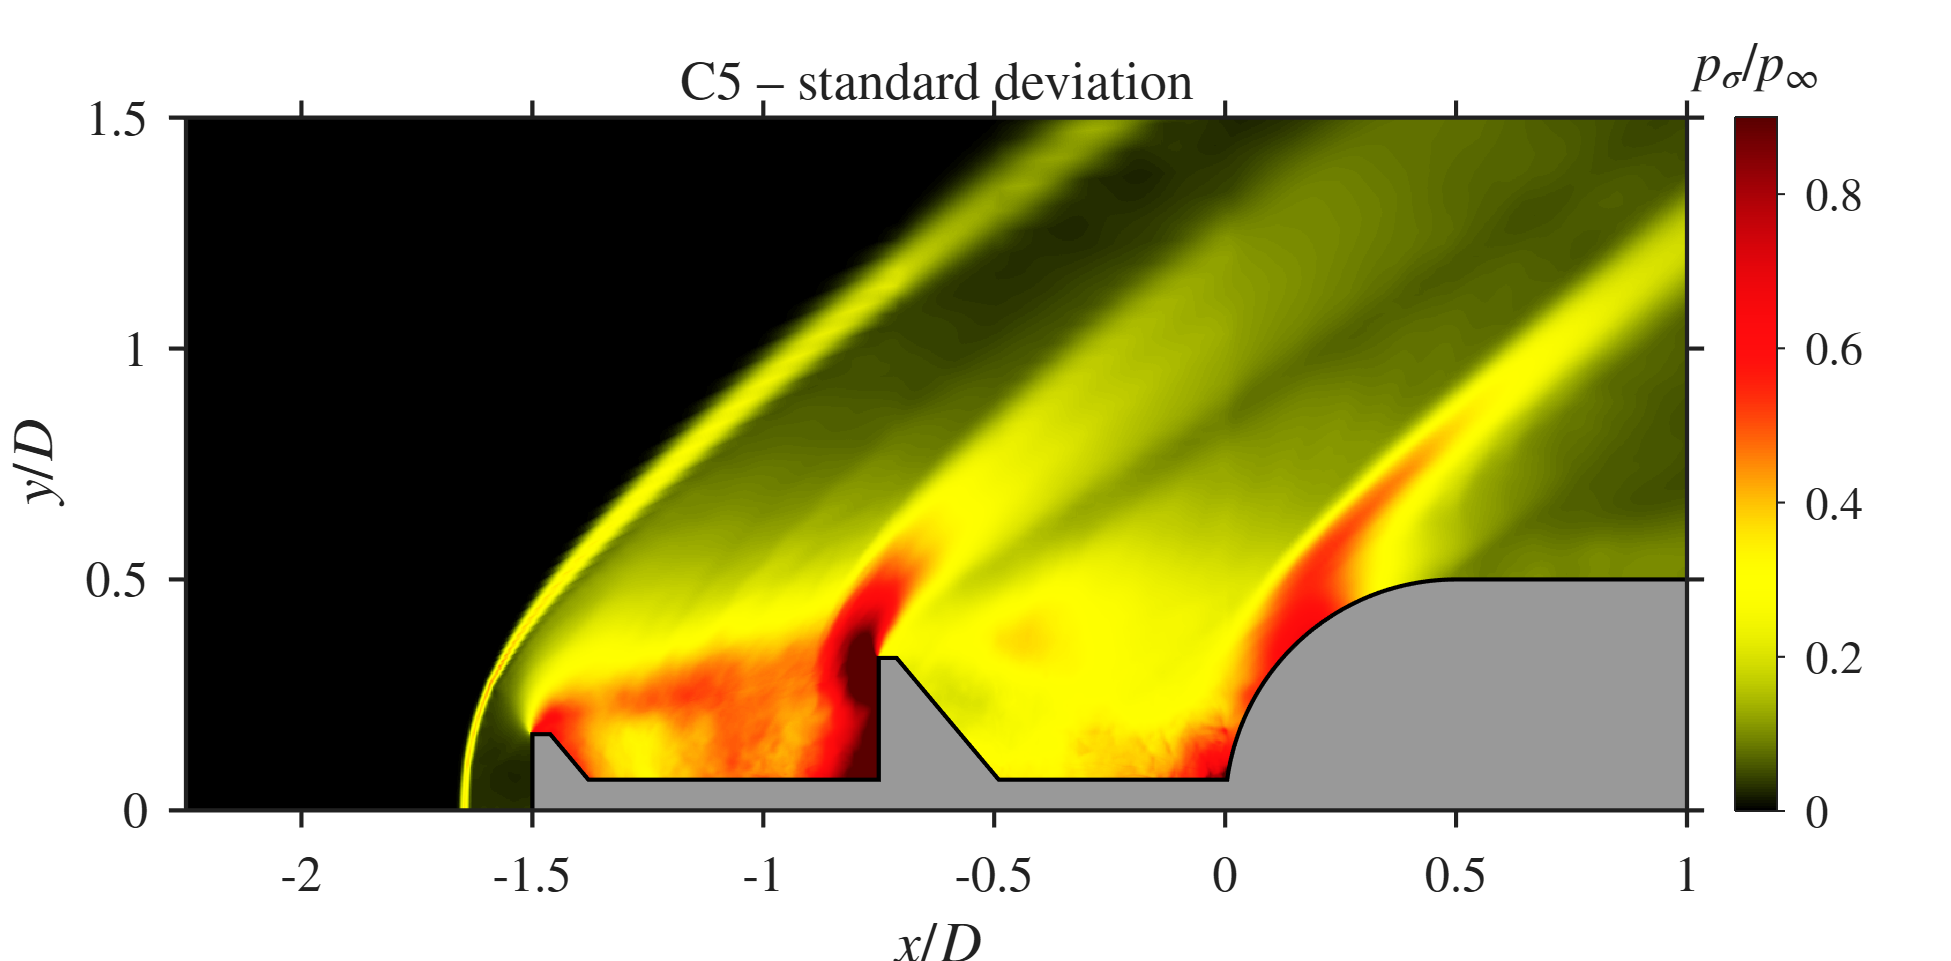
\includegraphics[width=\linewidth]{C5_std.png}\caption{C5, $\psd$}\end{subfigure}
  \caption{Disk-diameter sweep: mean pressure with streamlines (left) and pressure standard deviation (right).}
  \label{fig:dia_ms}
\end{figure}

\paragraph{Space-time behaviour.} Figures~\ref{fig:dia_xt} and~\ref{fig:dia_xf} show the $x$--$t$ and $x$--$f$ diagrams. In C4 the disk-face band sits at $St \approx 1.18$ and Cavity 2 carries $St \approx 0.83$, the same as the probe peak. In C5 the disk-face band drops to $St \approx 0.29$, matching the leading SPOD mode, while Cavity 2 carries $St \approx 0.74$, close to the SA tone.

\begin{figure}[htbp]
  \centering
  \begin{subfigure}{0.325\textwidth}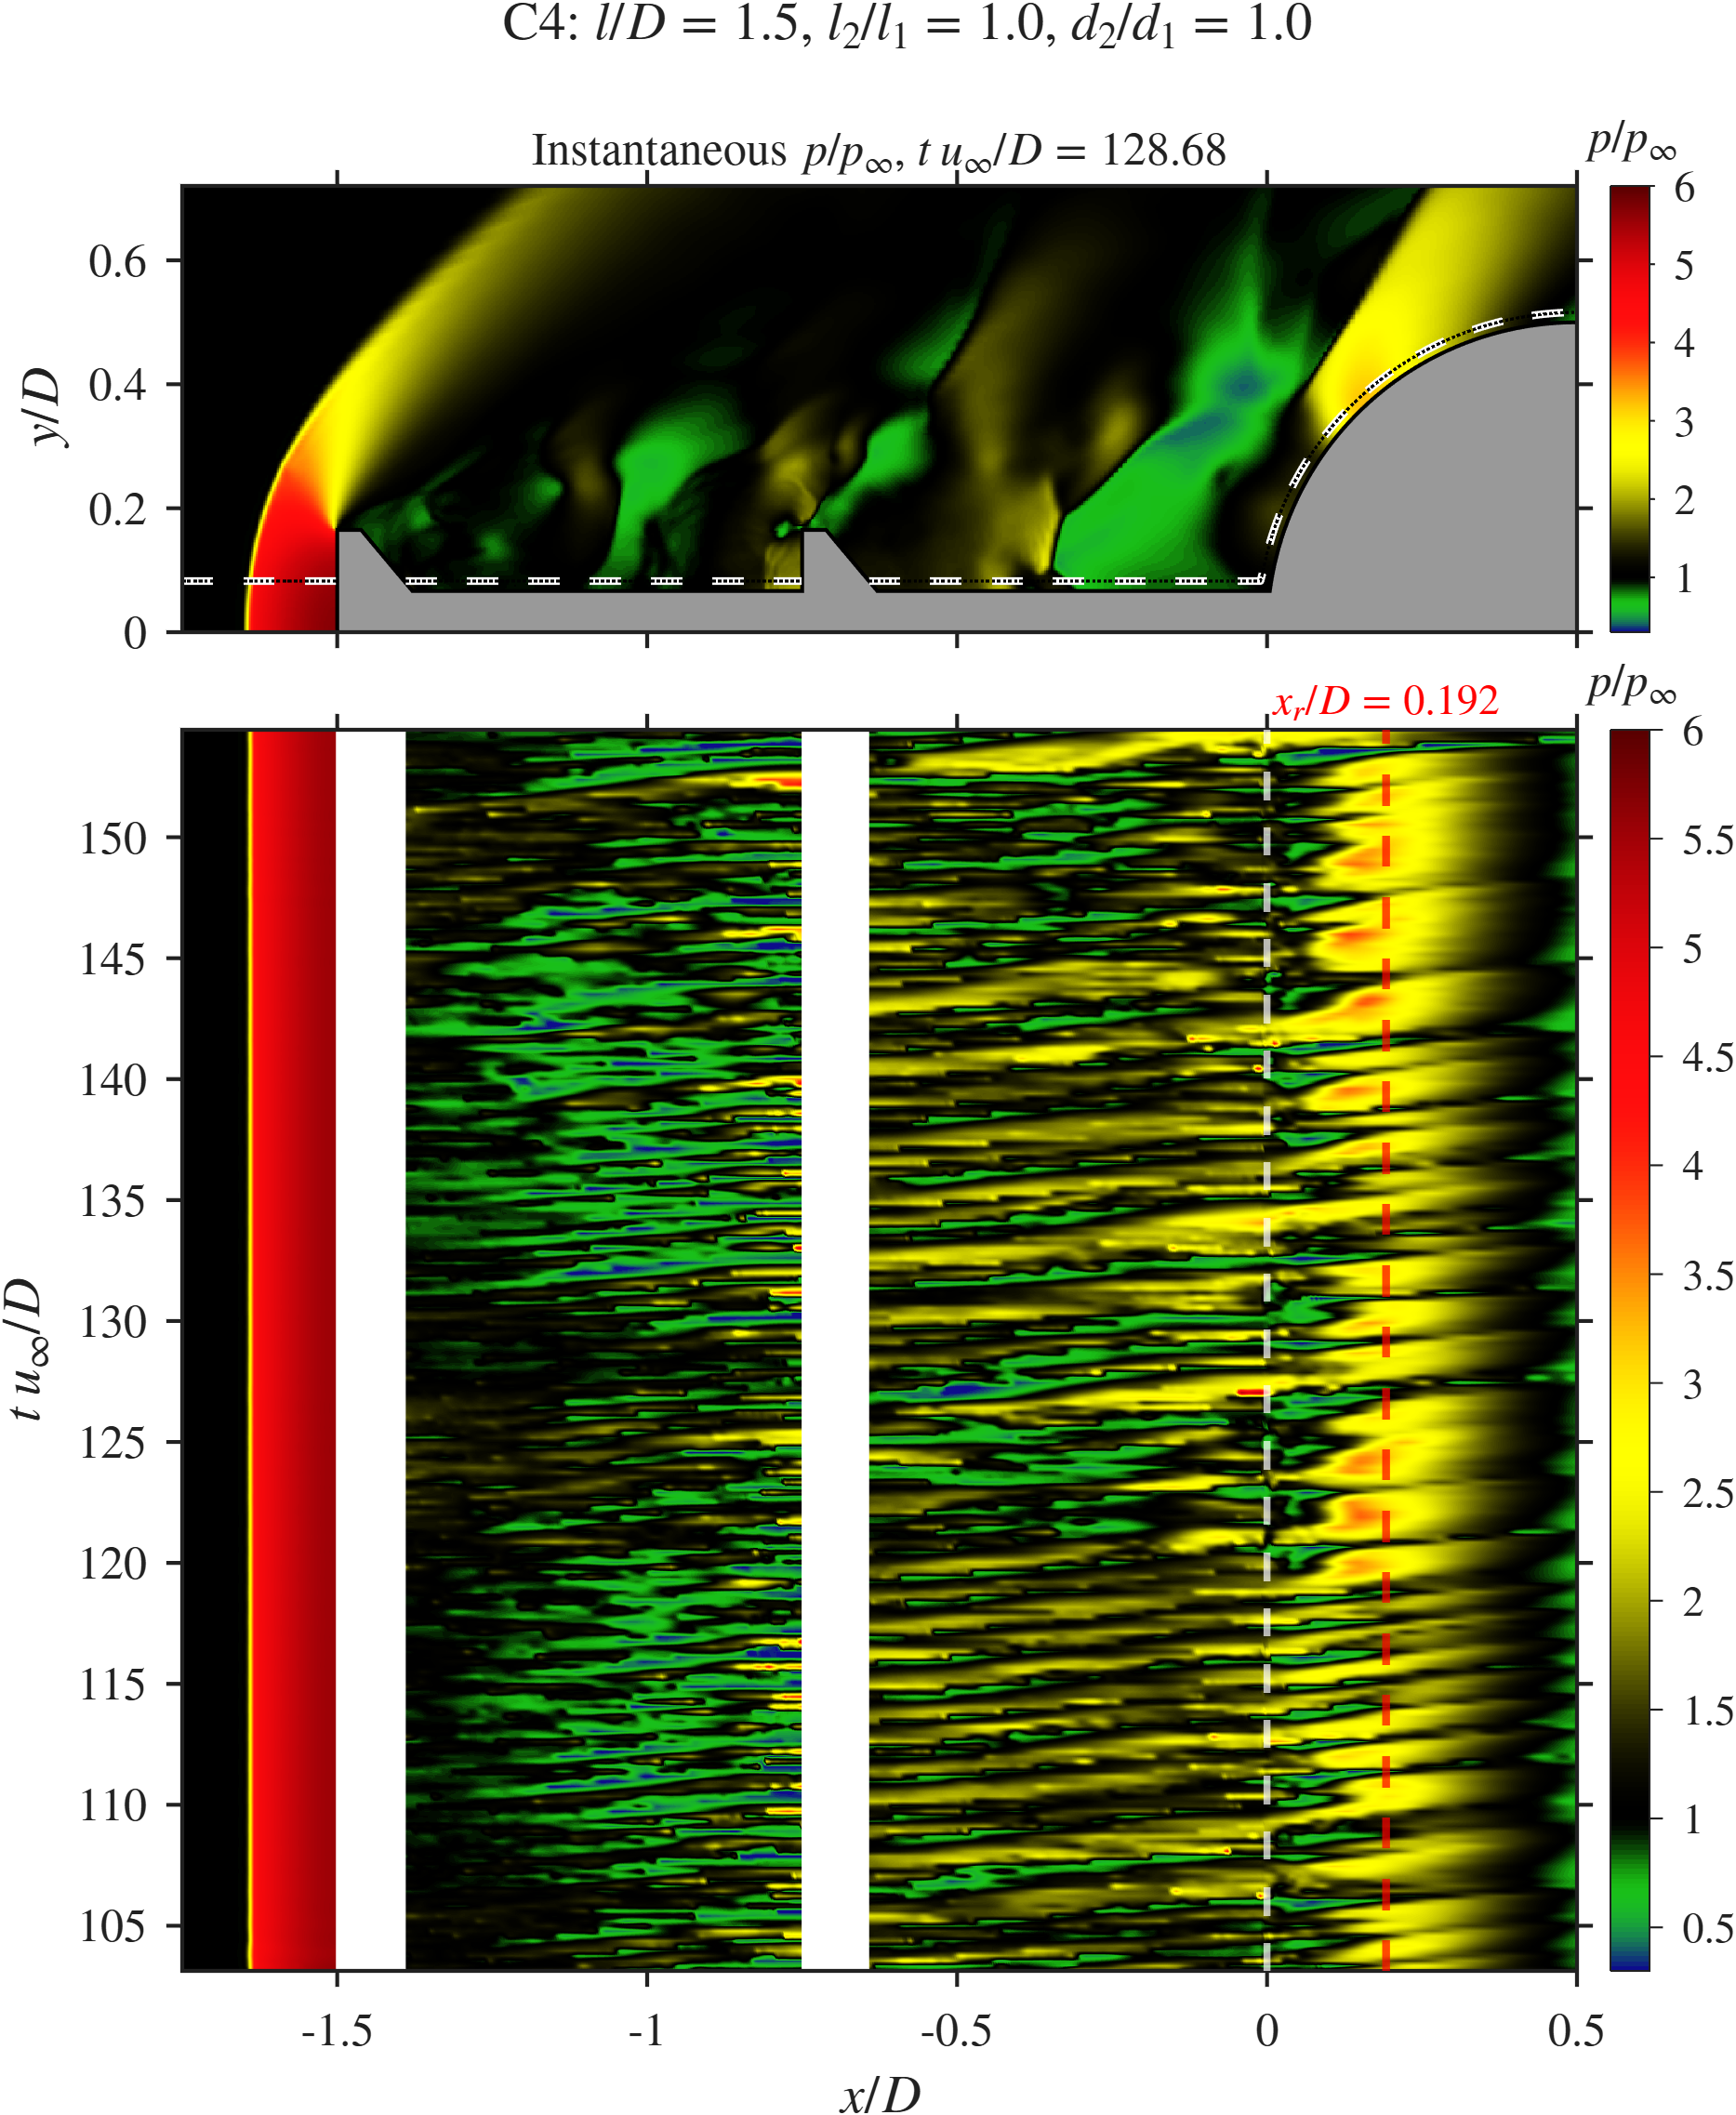
\includegraphics[width=\linewidth]{C4_xt.png}\caption{C4}\end{subfigure}
  \begin{subfigure}{0.325\textwidth}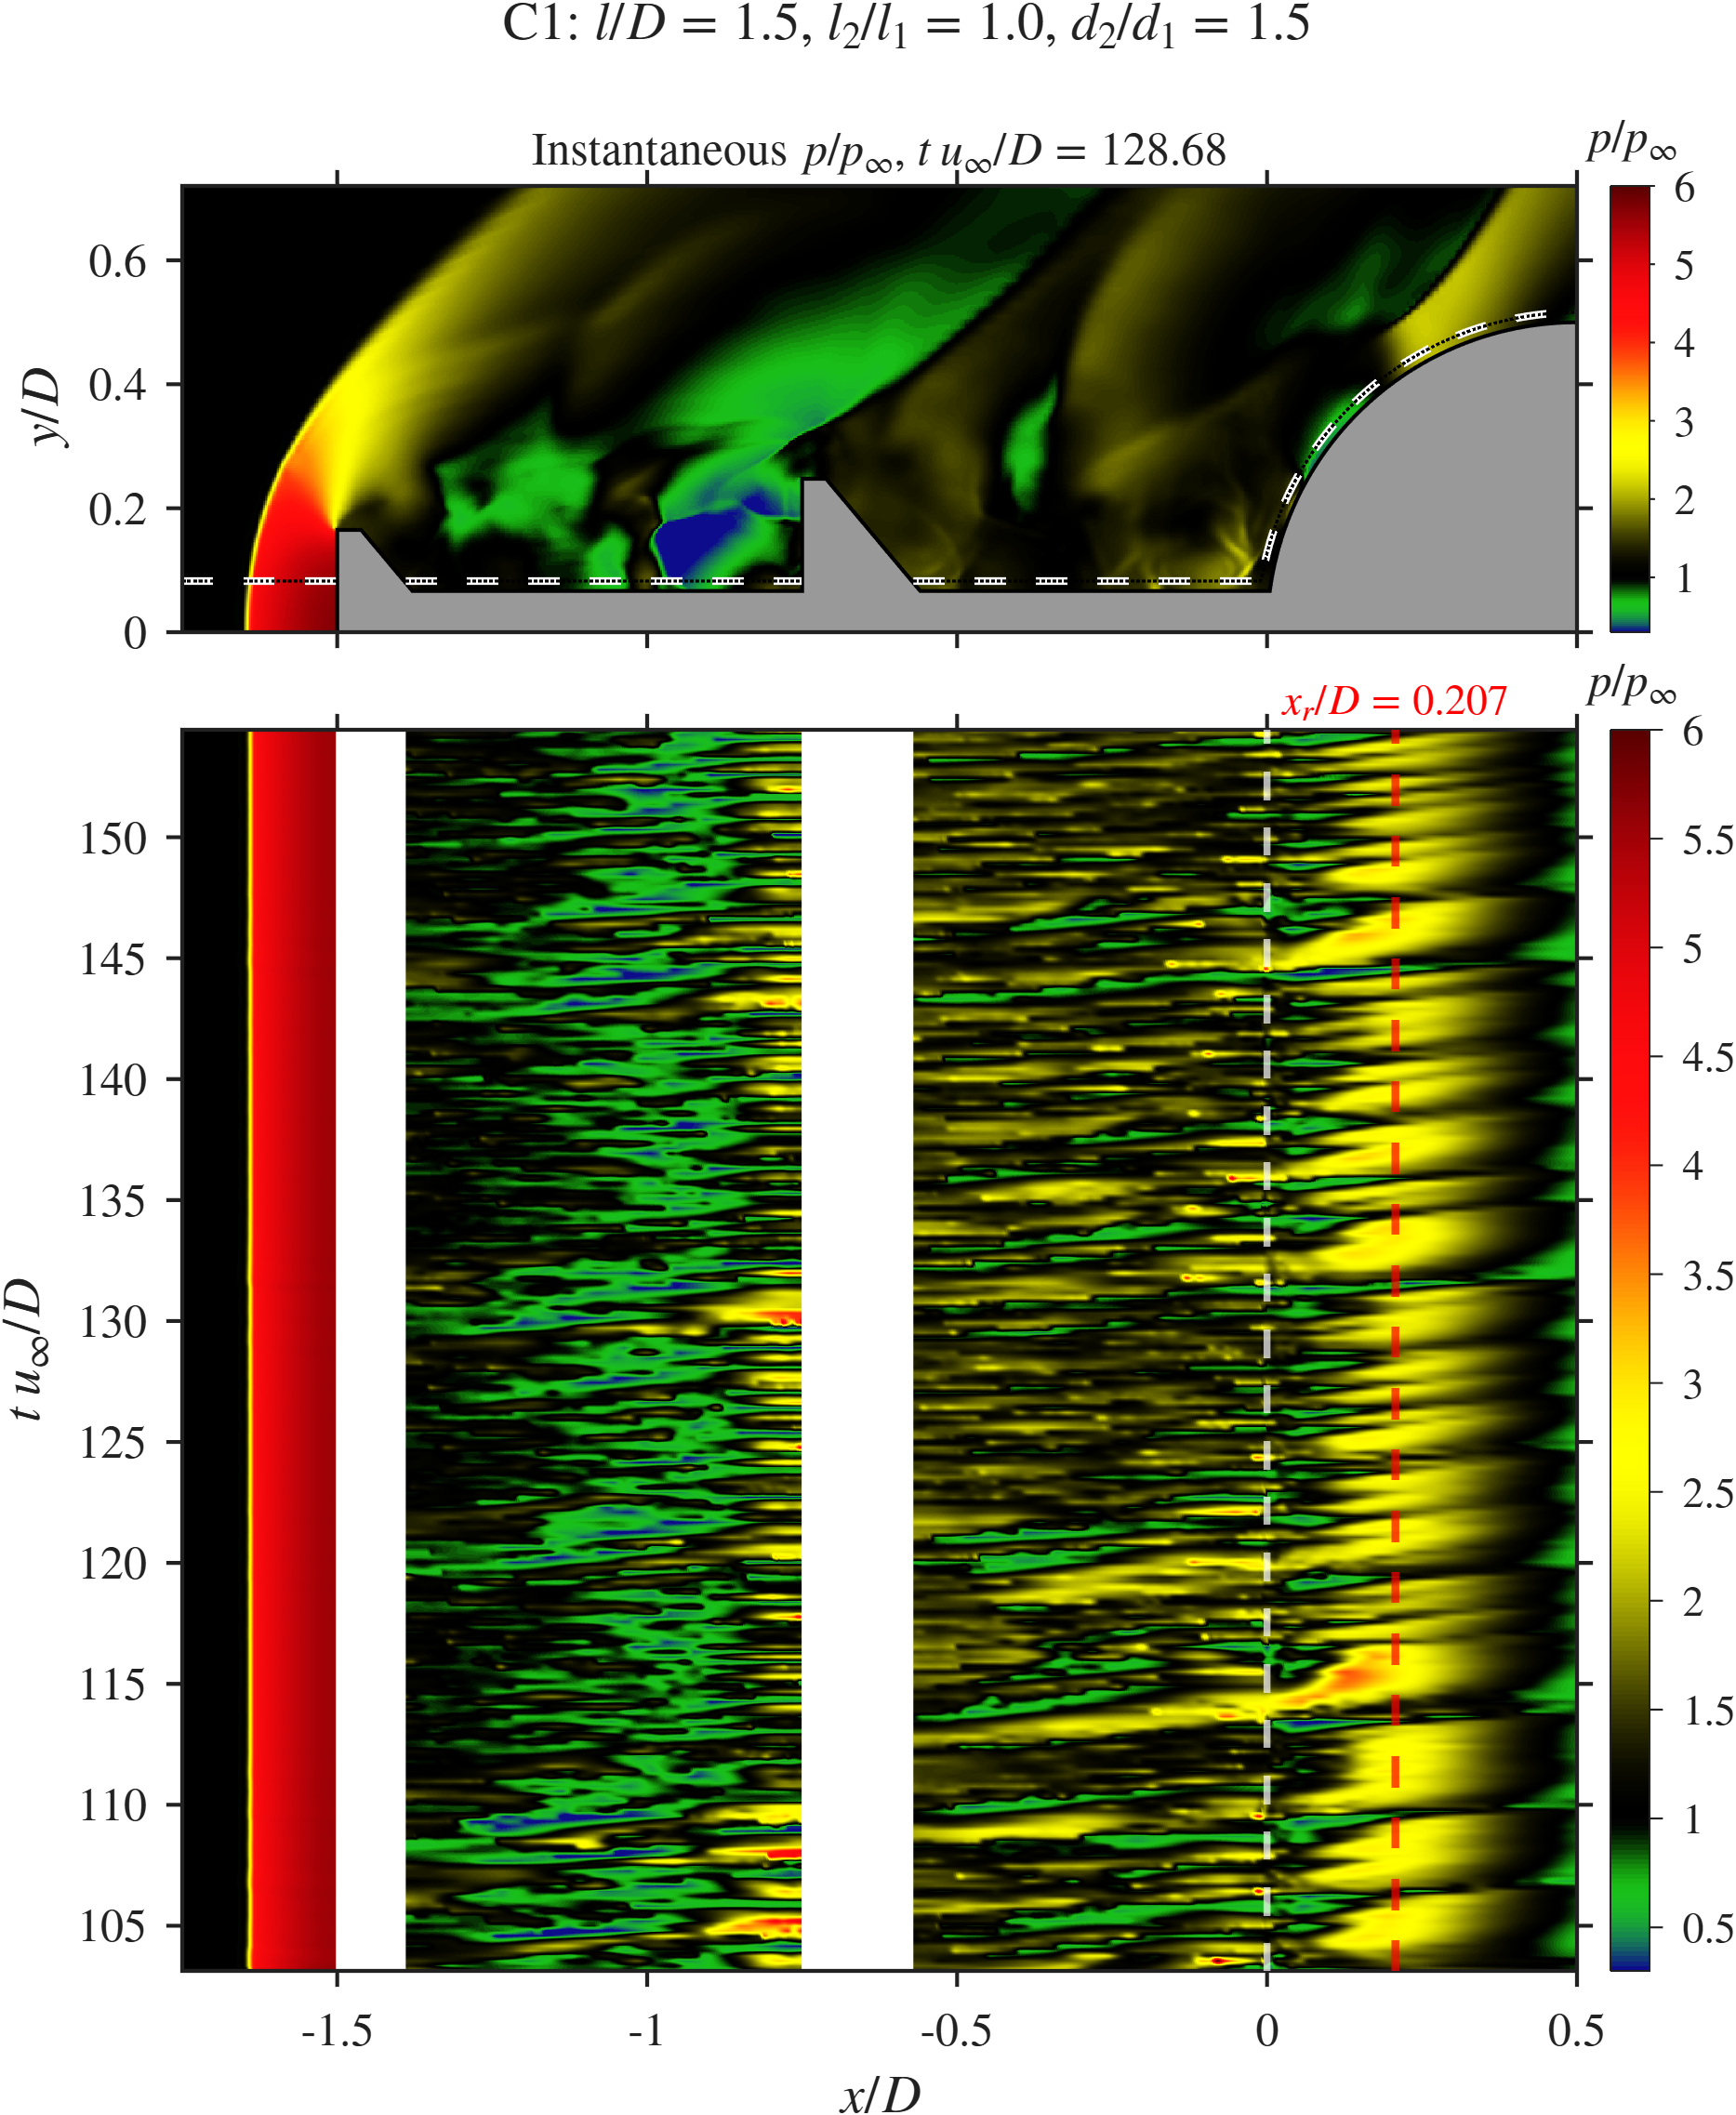
\includegraphics[width=\linewidth]{C1_xt.png}\caption{C1}\end{subfigure}
  \begin{subfigure}{0.325\textwidth}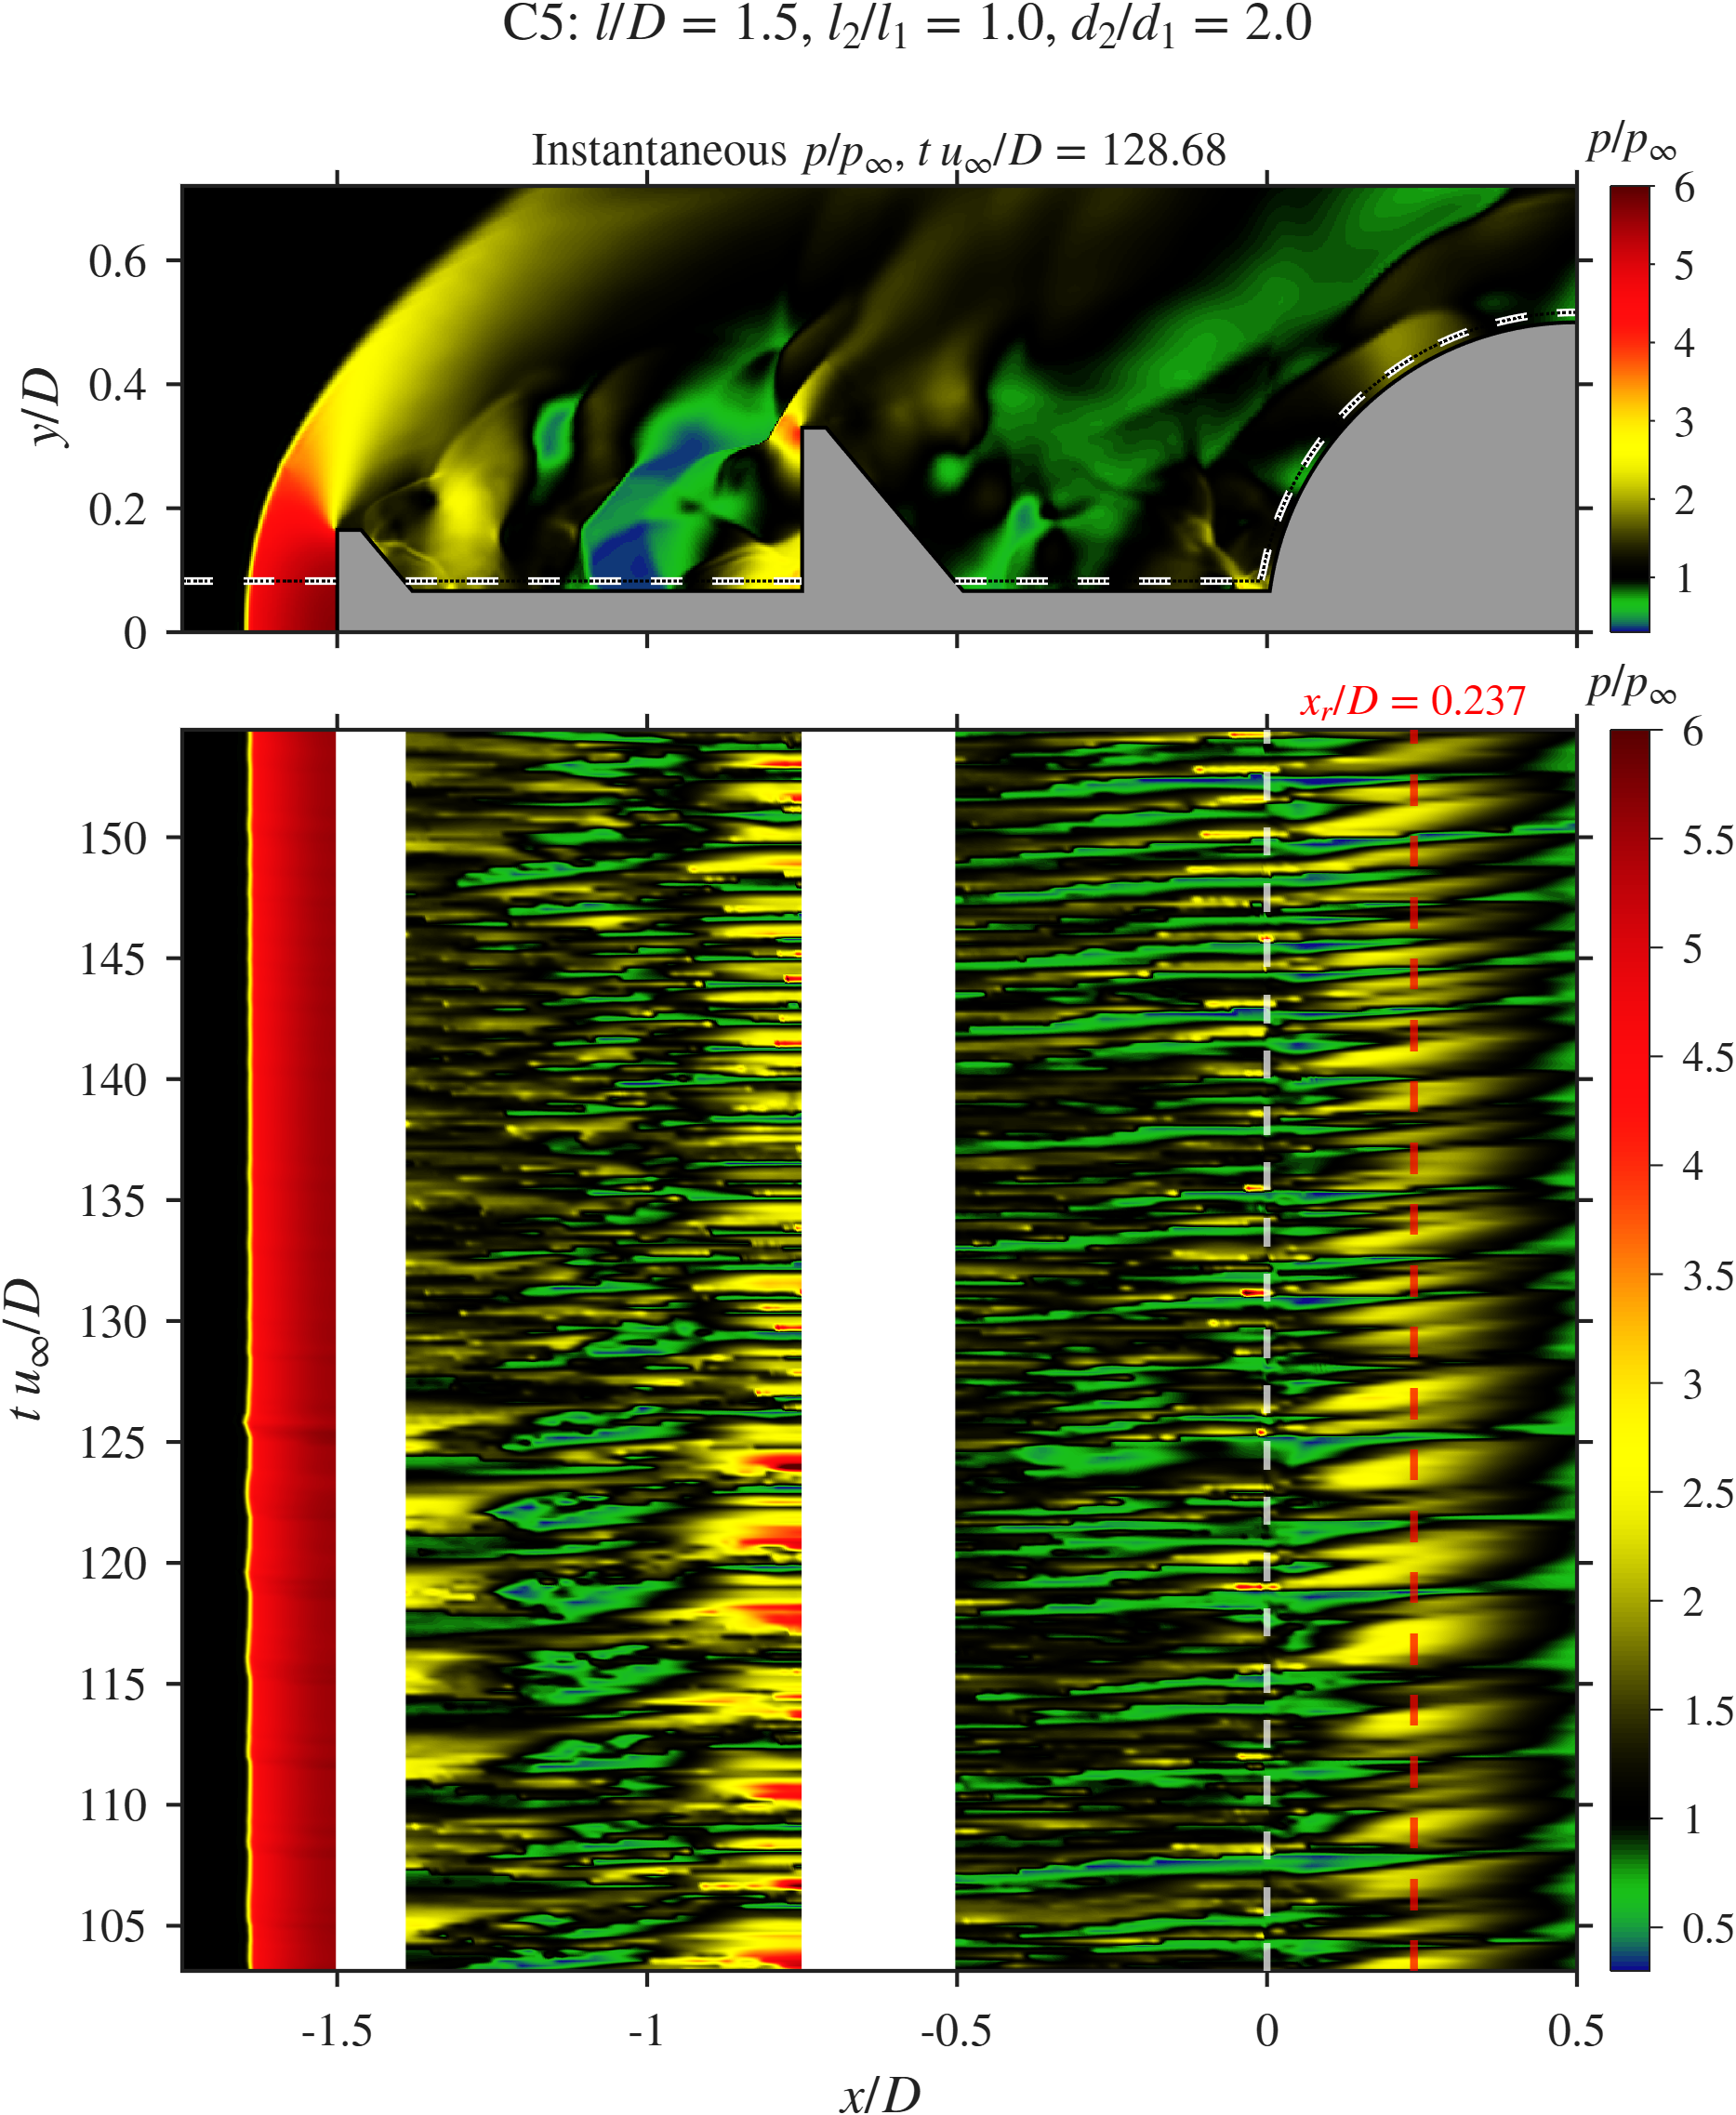
\includegraphics[width=\linewidth]{C5_xt.png}\caption{C5}\end{subfigure}
  \caption{Disk-diameter sweep: $x$--$t$ diagrams of $p/\pinf$ along the probe line.}
  \label{fig:dia_xt}
\end{figure}

\begin{figure}[htbp]
  \centering
  \begin{subfigure}{0.325\textwidth}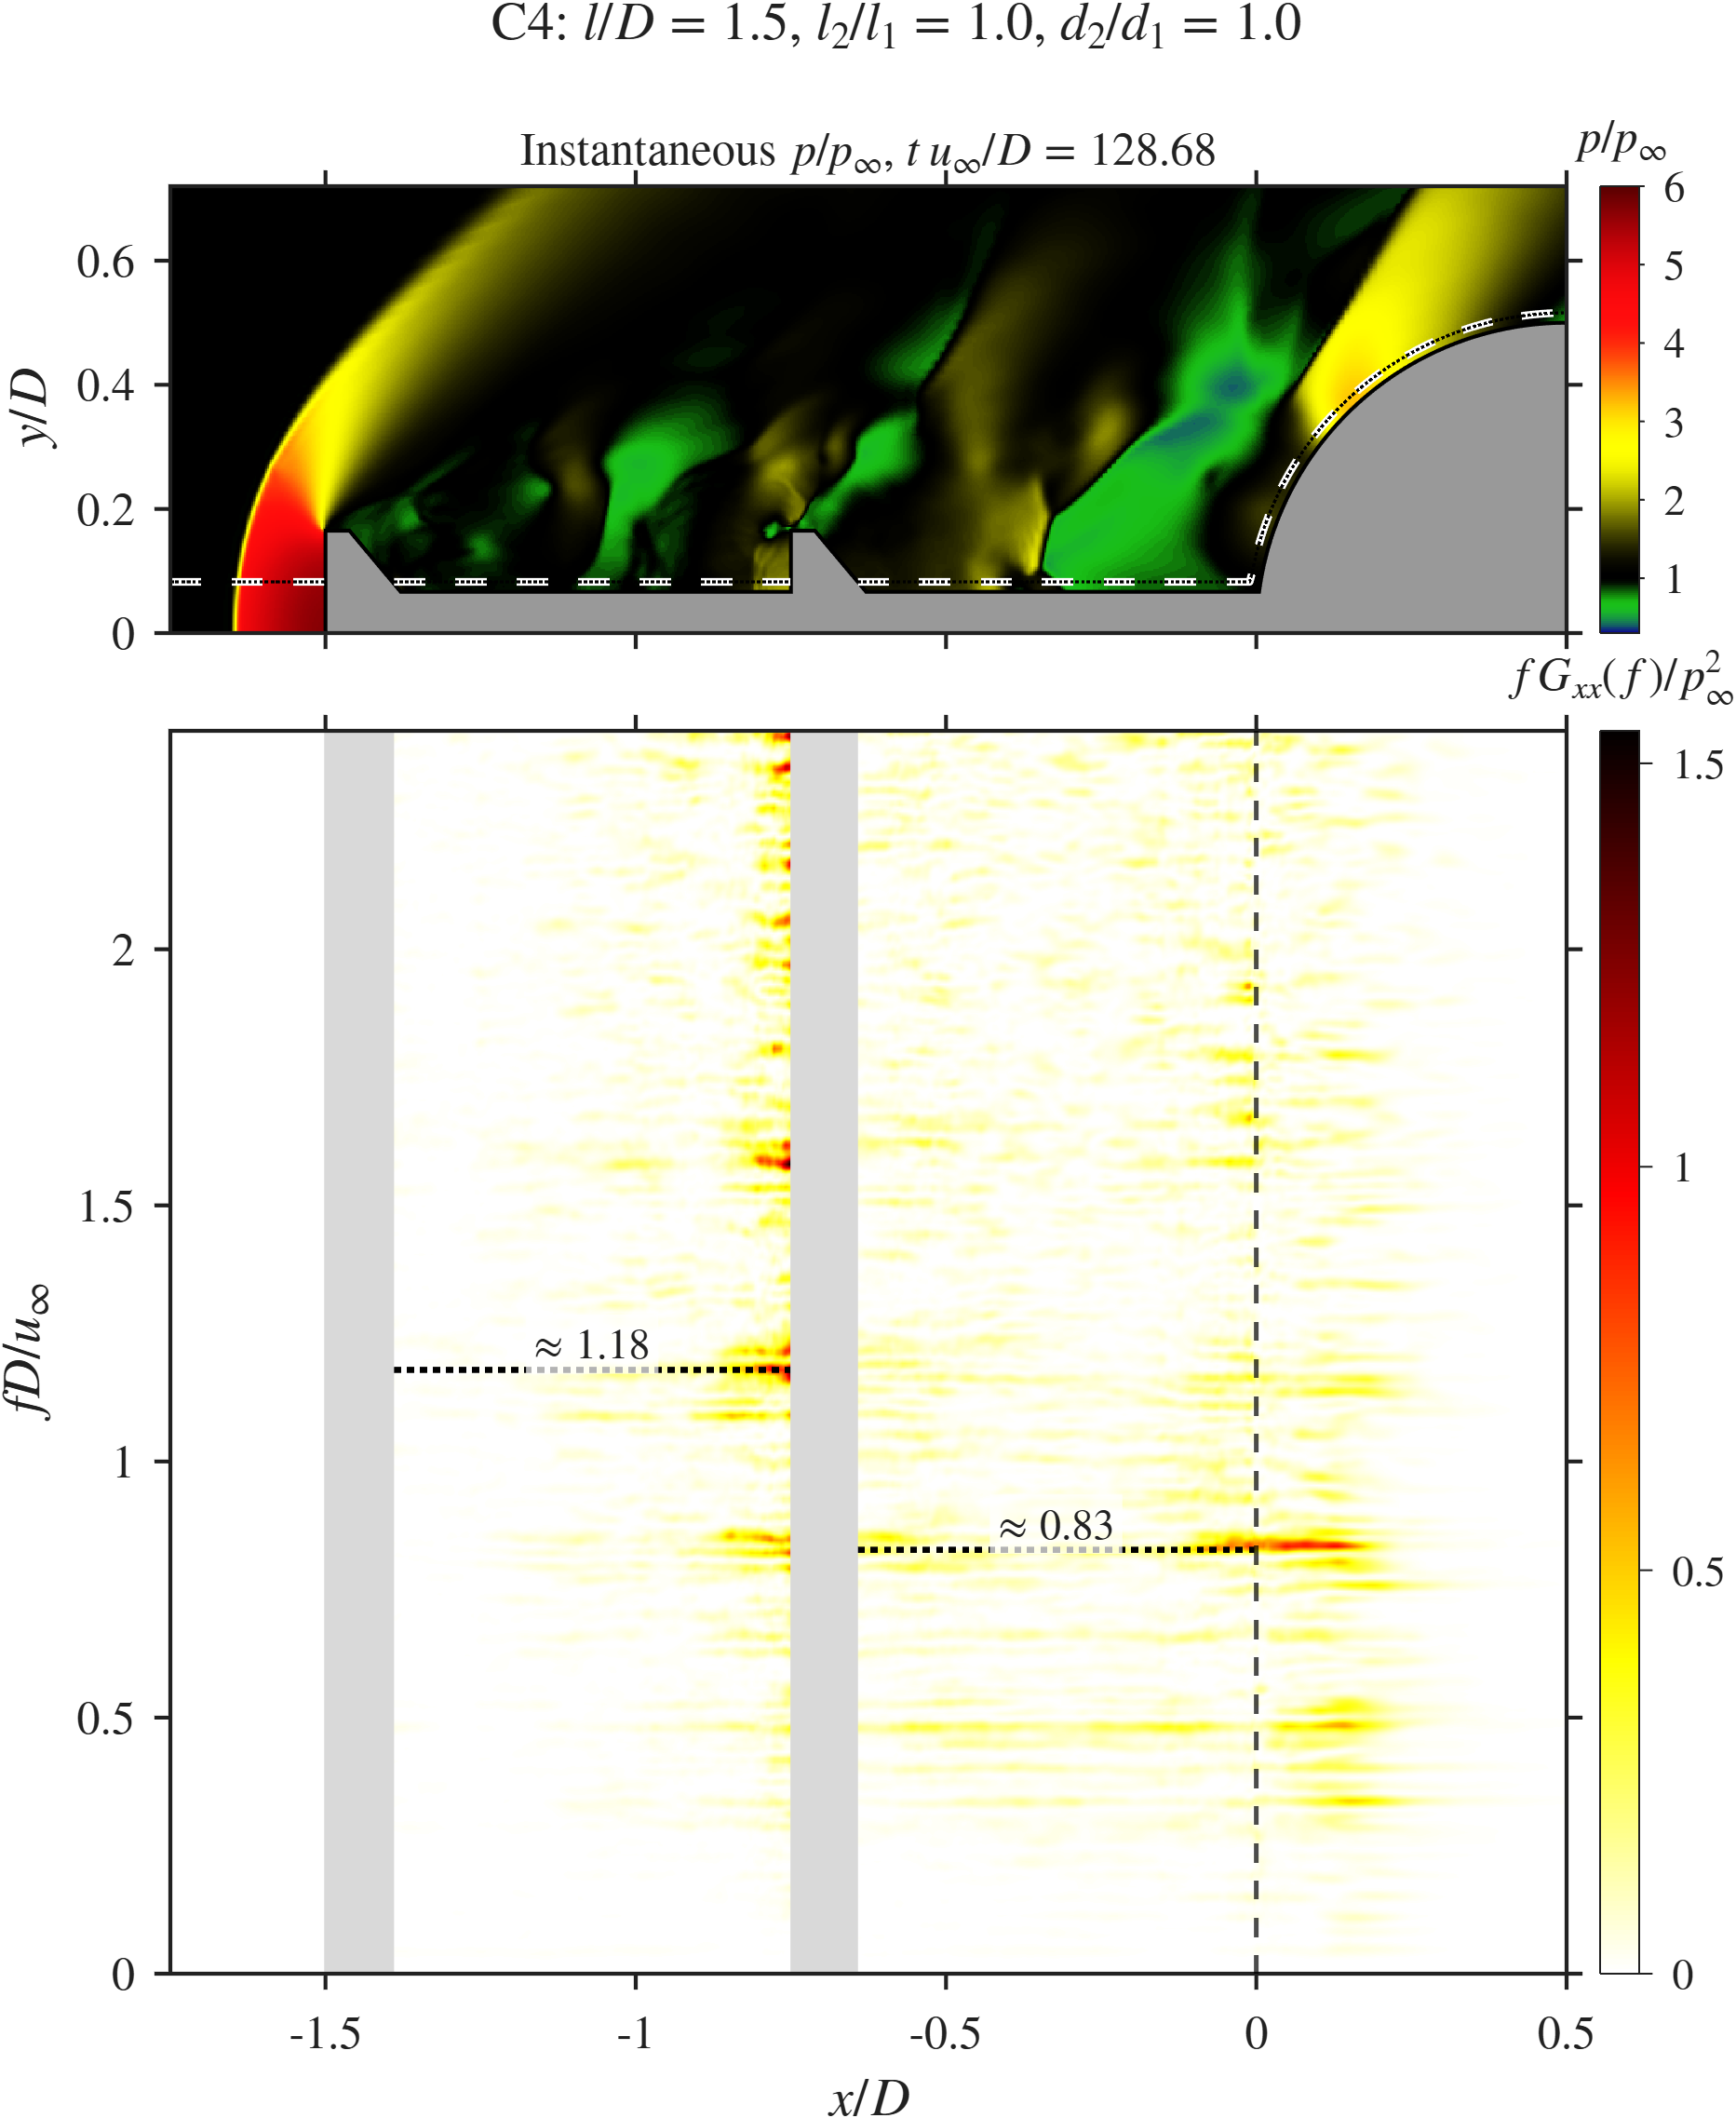
\includegraphics[width=\linewidth]{C4_xf.png}\caption{C4}\end{subfigure}
  \begin{subfigure}{0.325\textwidth}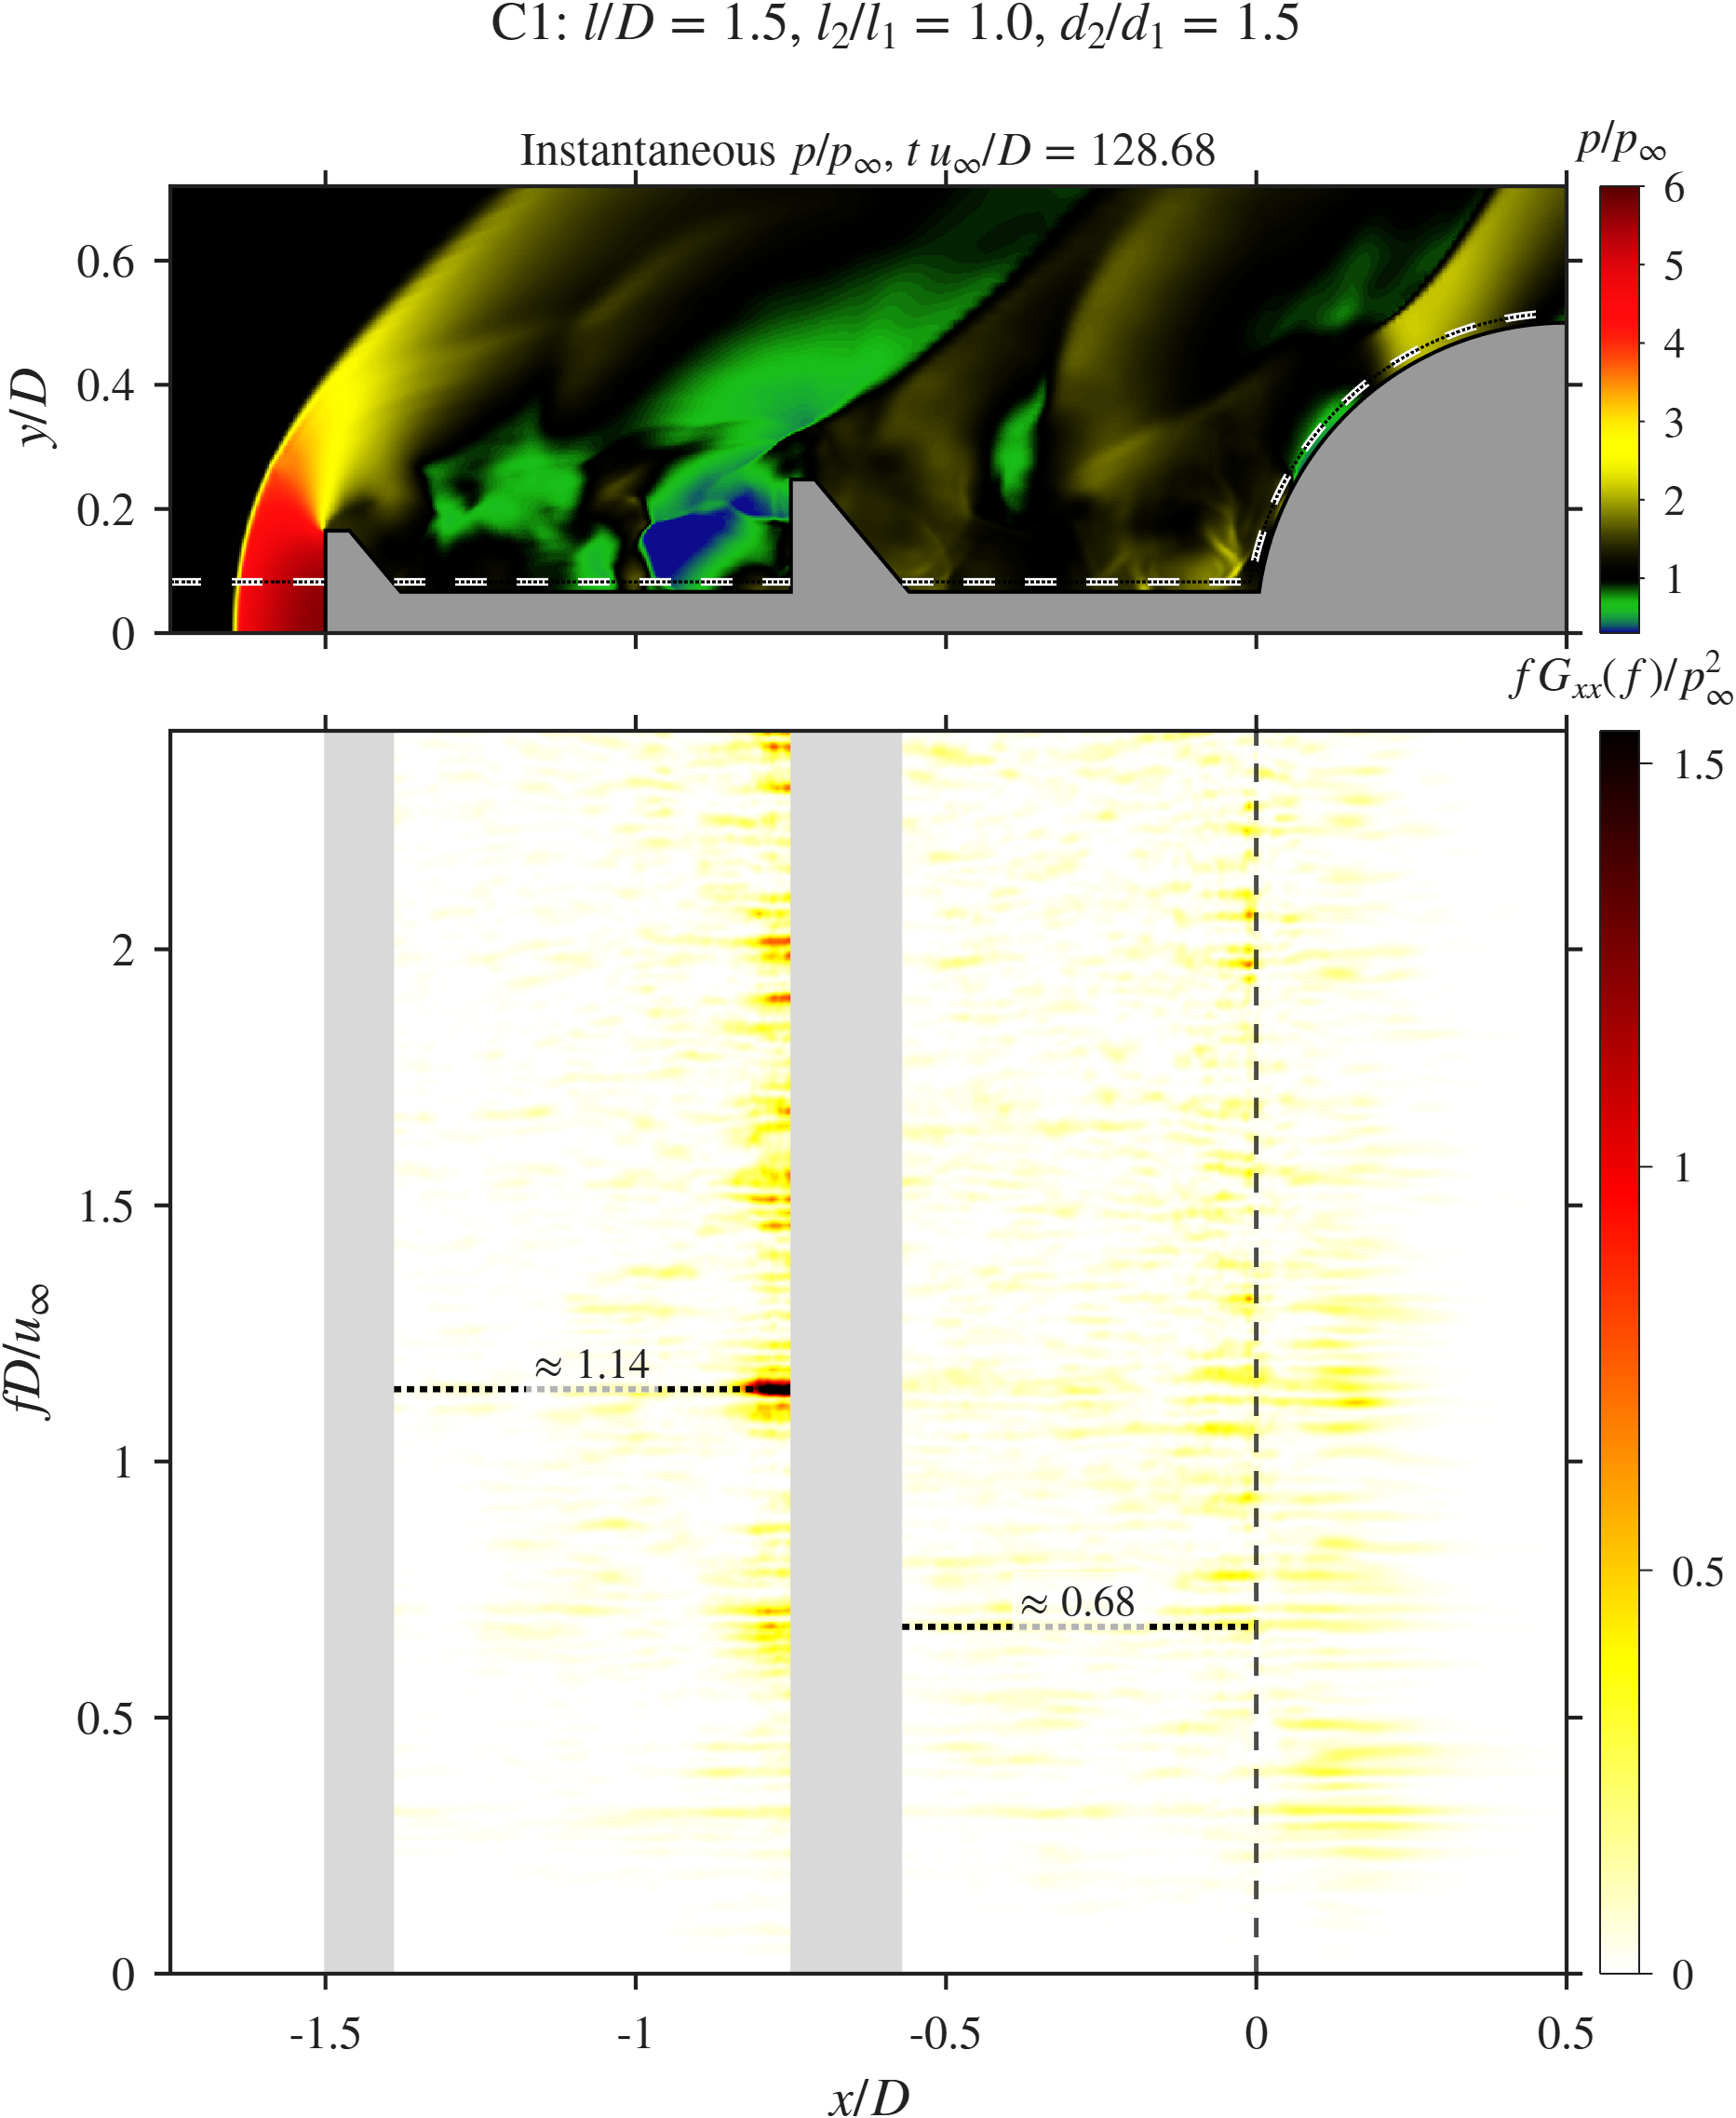
\includegraphics[width=\linewidth]{C1_xf.png}\caption{C1}\end{subfigure}
  \begin{subfigure}{0.325\textwidth}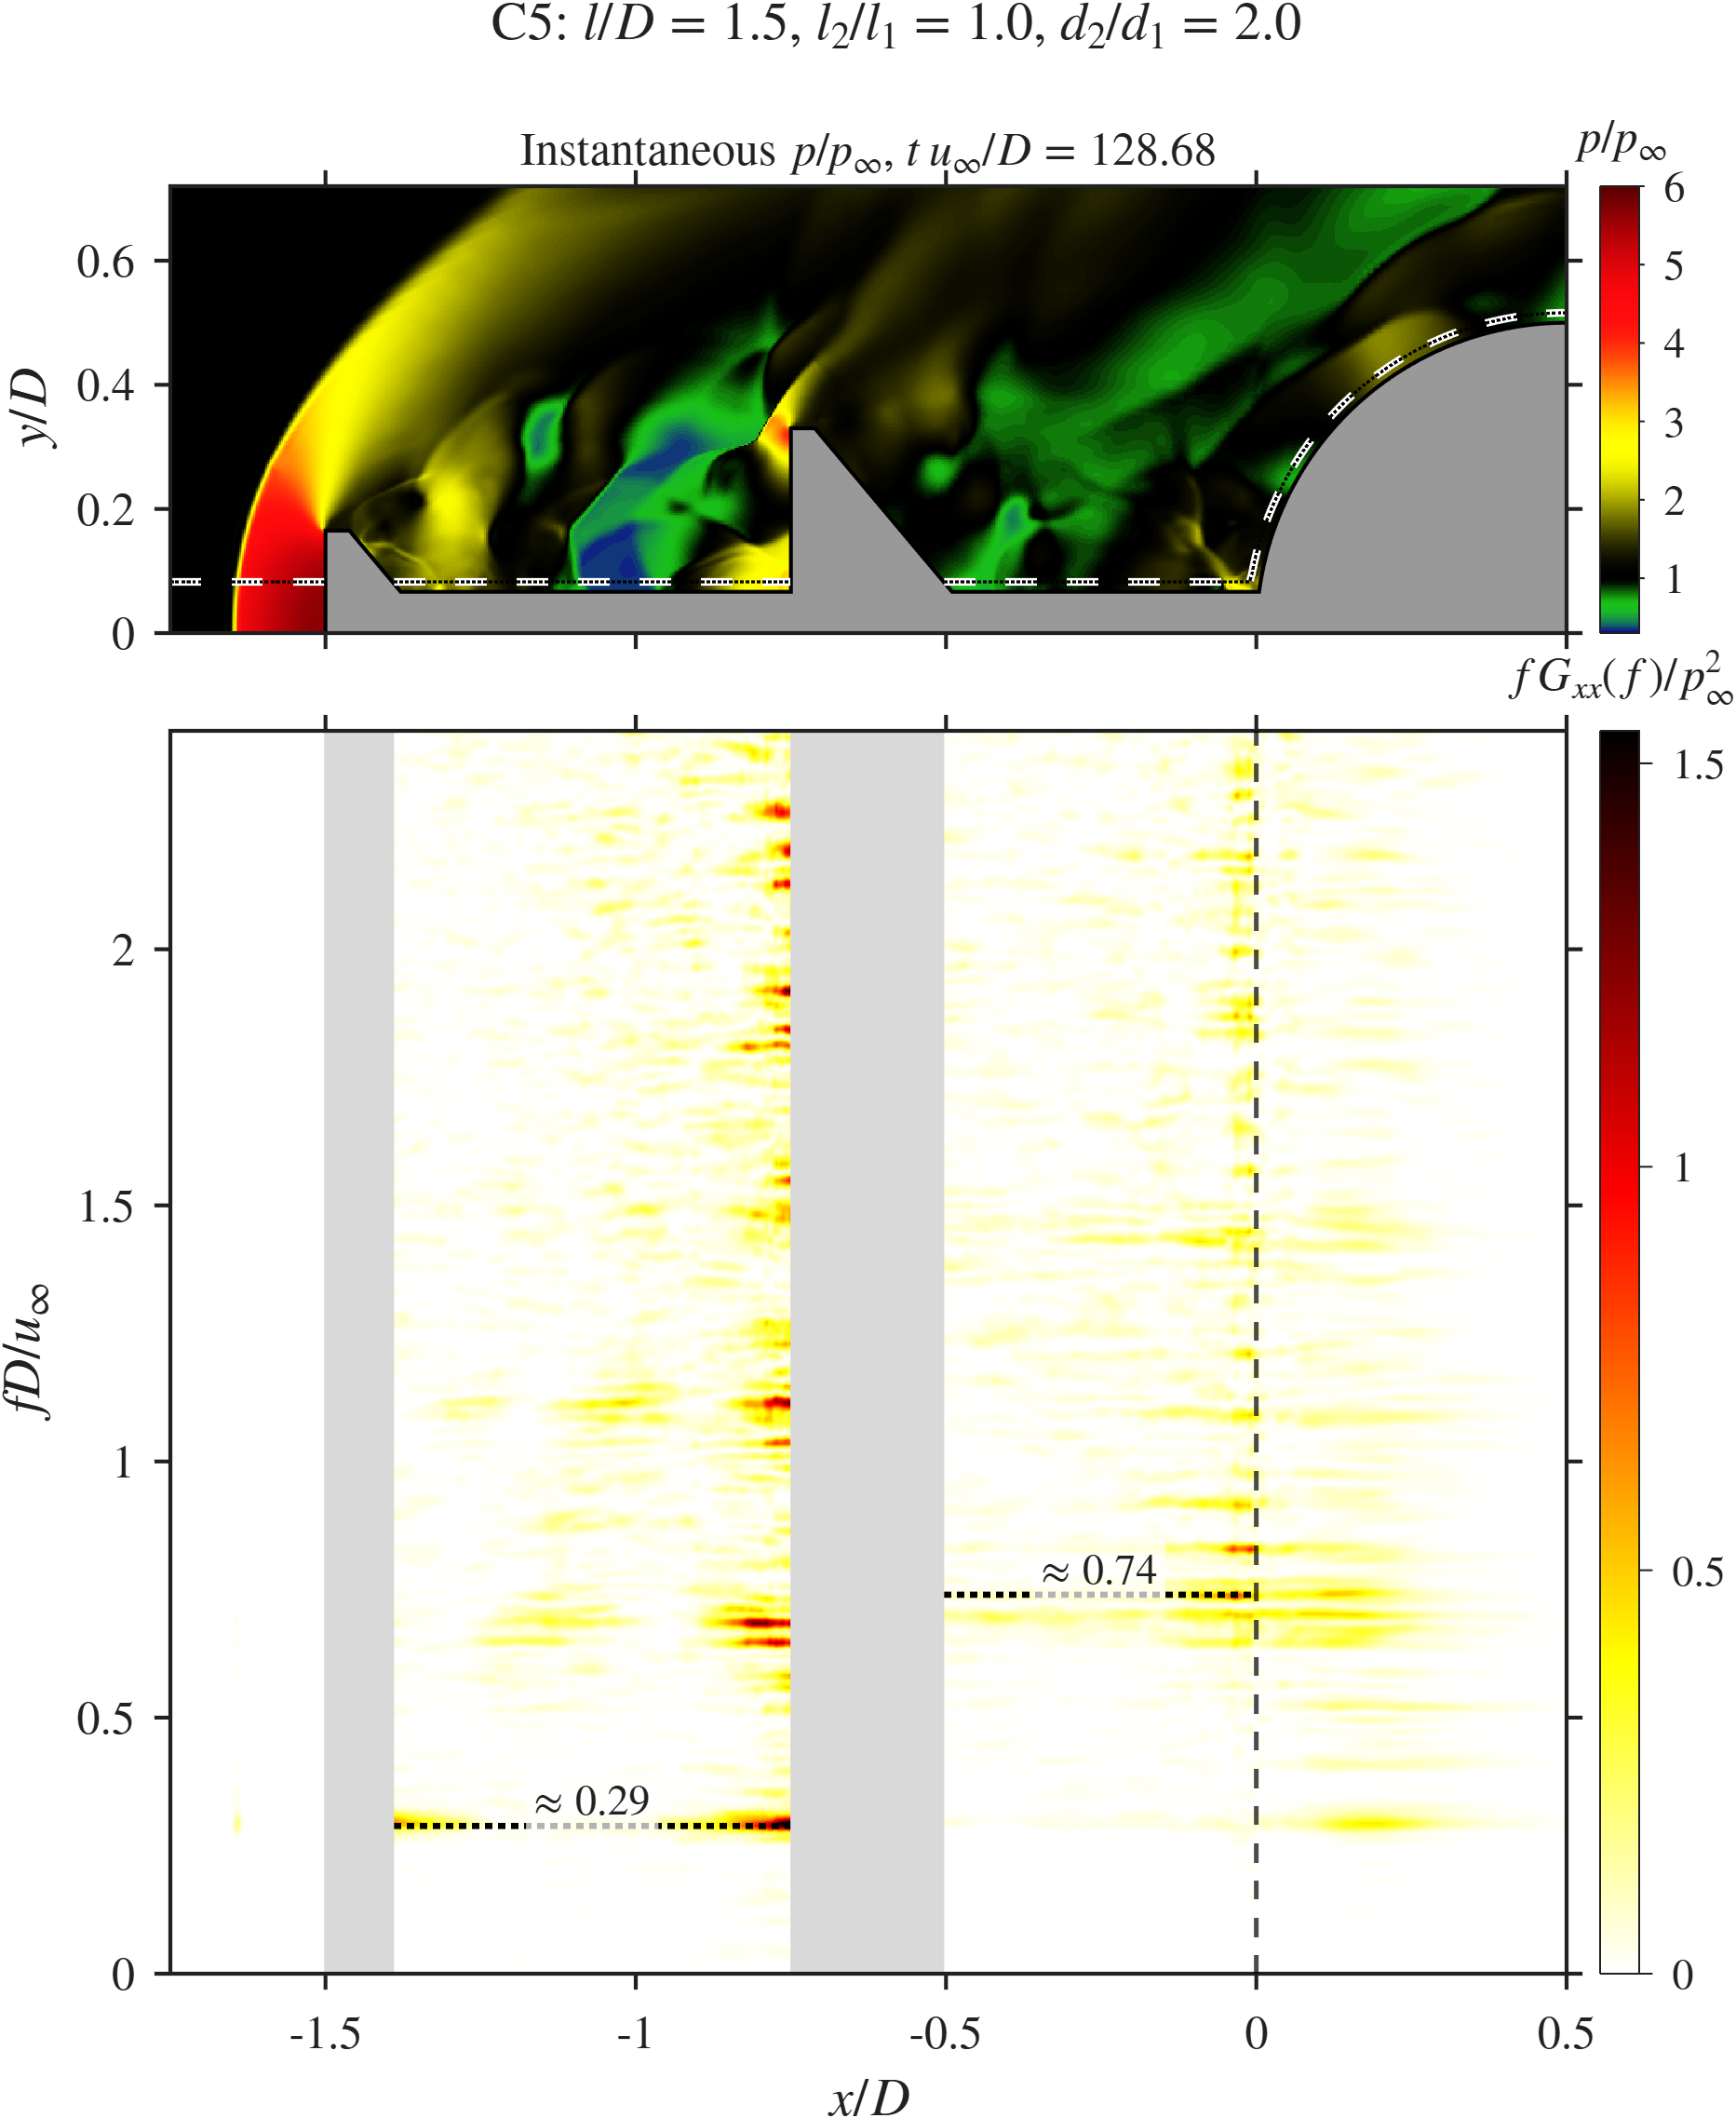
\includegraphics[width=\linewidth]{C5_xf.png}\caption{C5}\end{subfigure}
  \caption{Disk-diameter sweep: $x$--$f$ diagrams along the probe line.}
  \label{fig:dia_xf}
\end{figure}

\paragraph{Probe signals and spectra.} Figure~\ref{fig:dia_sig} shows the signals. C4 has a peak at $St = 0.83$ with $\Pi \approx 0.72$, the highest peak of any DDAS case, though still about 80\% below SA. Its frequency is close to the SA tone (0.76), and its pressure and drag peaks coincide ($St = 0.83$), so the equal disk keeps a single-cavity loop. C1 has the broad spectrum described above. C5 has a peak at $St = 0.74$ with $\Pi \approx 0.44$, again close to SA, but its pressure and drag peaks separate ($St = 0.74$ and 0.65). C5 and C1 have the same mean drag ($\Cdm = 0.39$), yet the drag fluctuation of C5 ($\sCd = 0.20$) is 67\% higher than C1 and the highest of all cases. The large second disk shields the shoulder from mean load, but its unsteady face loading adds to the drag oscillation.

\begin{figure}[htbp]
  \centering
  \begin{subfigure}{\textwidth}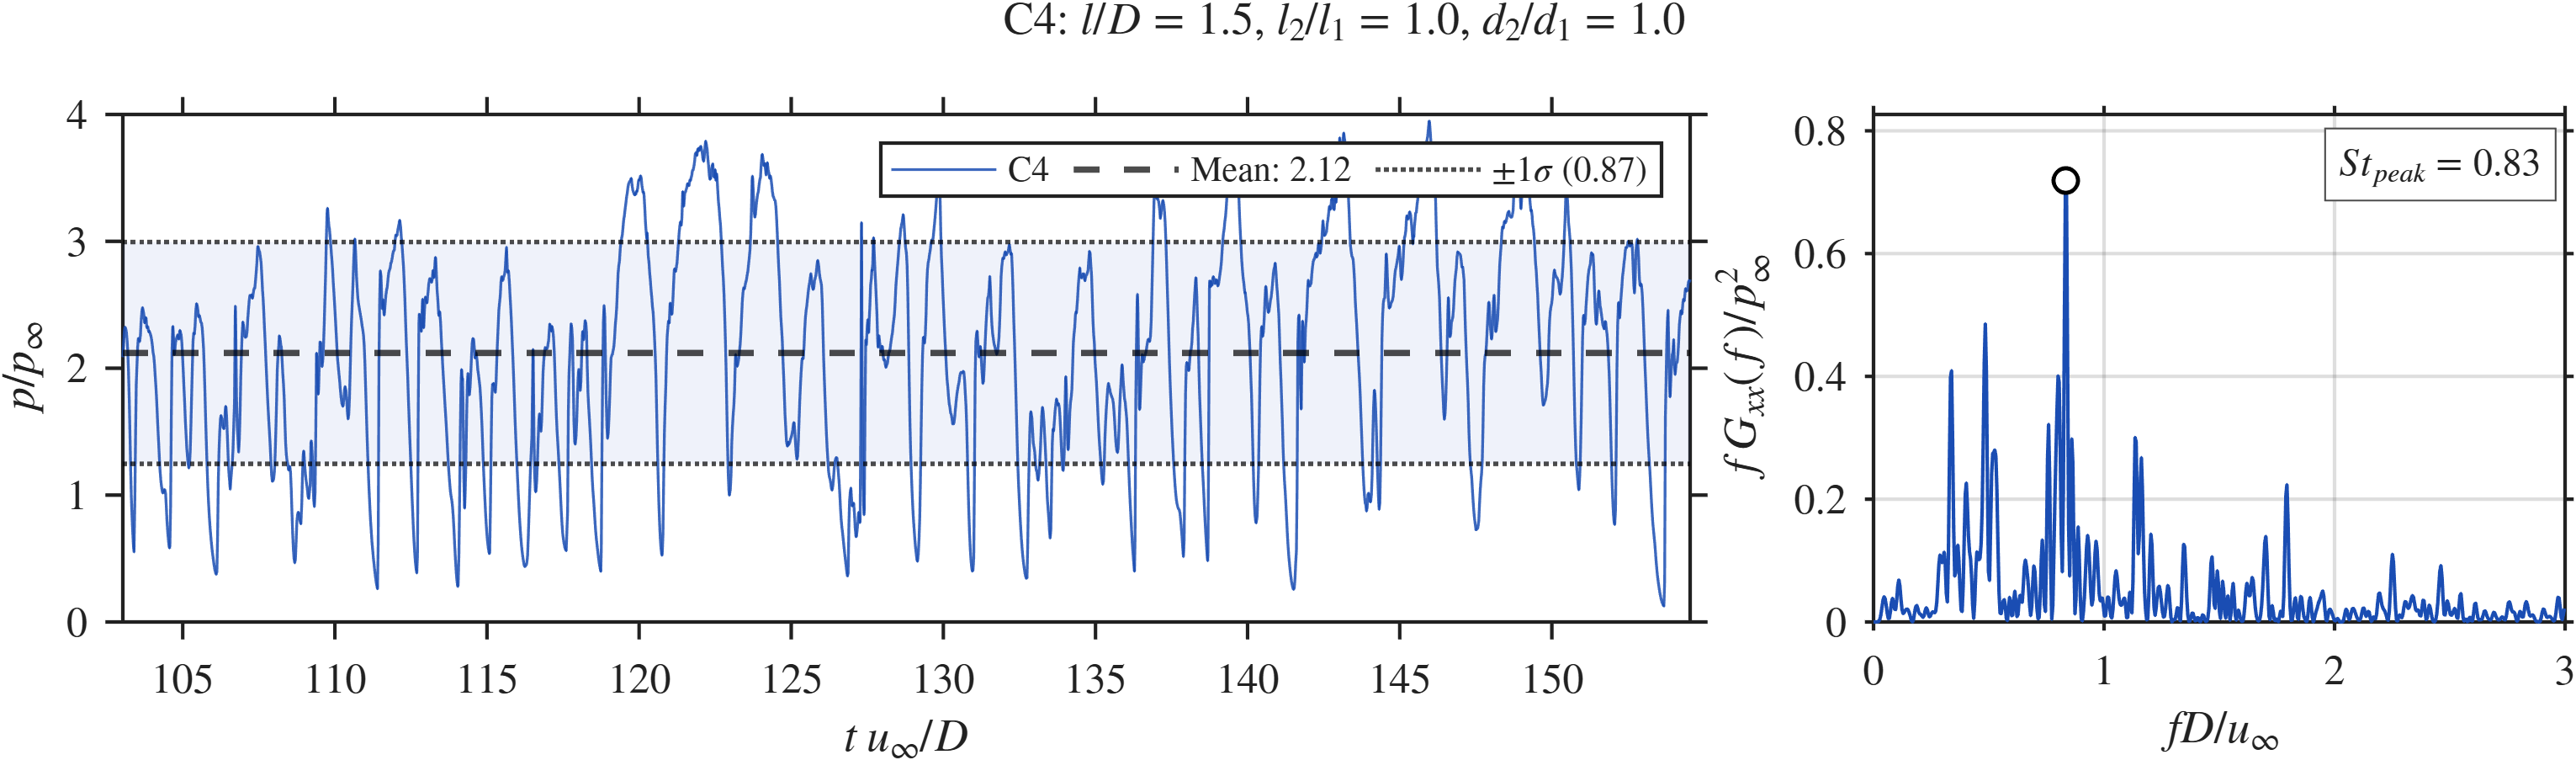
\includegraphics[width=\linewidth]{C4_psig.png}\caption{C4, pressure}\end{subfigure}\\
  \begin{subfigure}{\textwidth}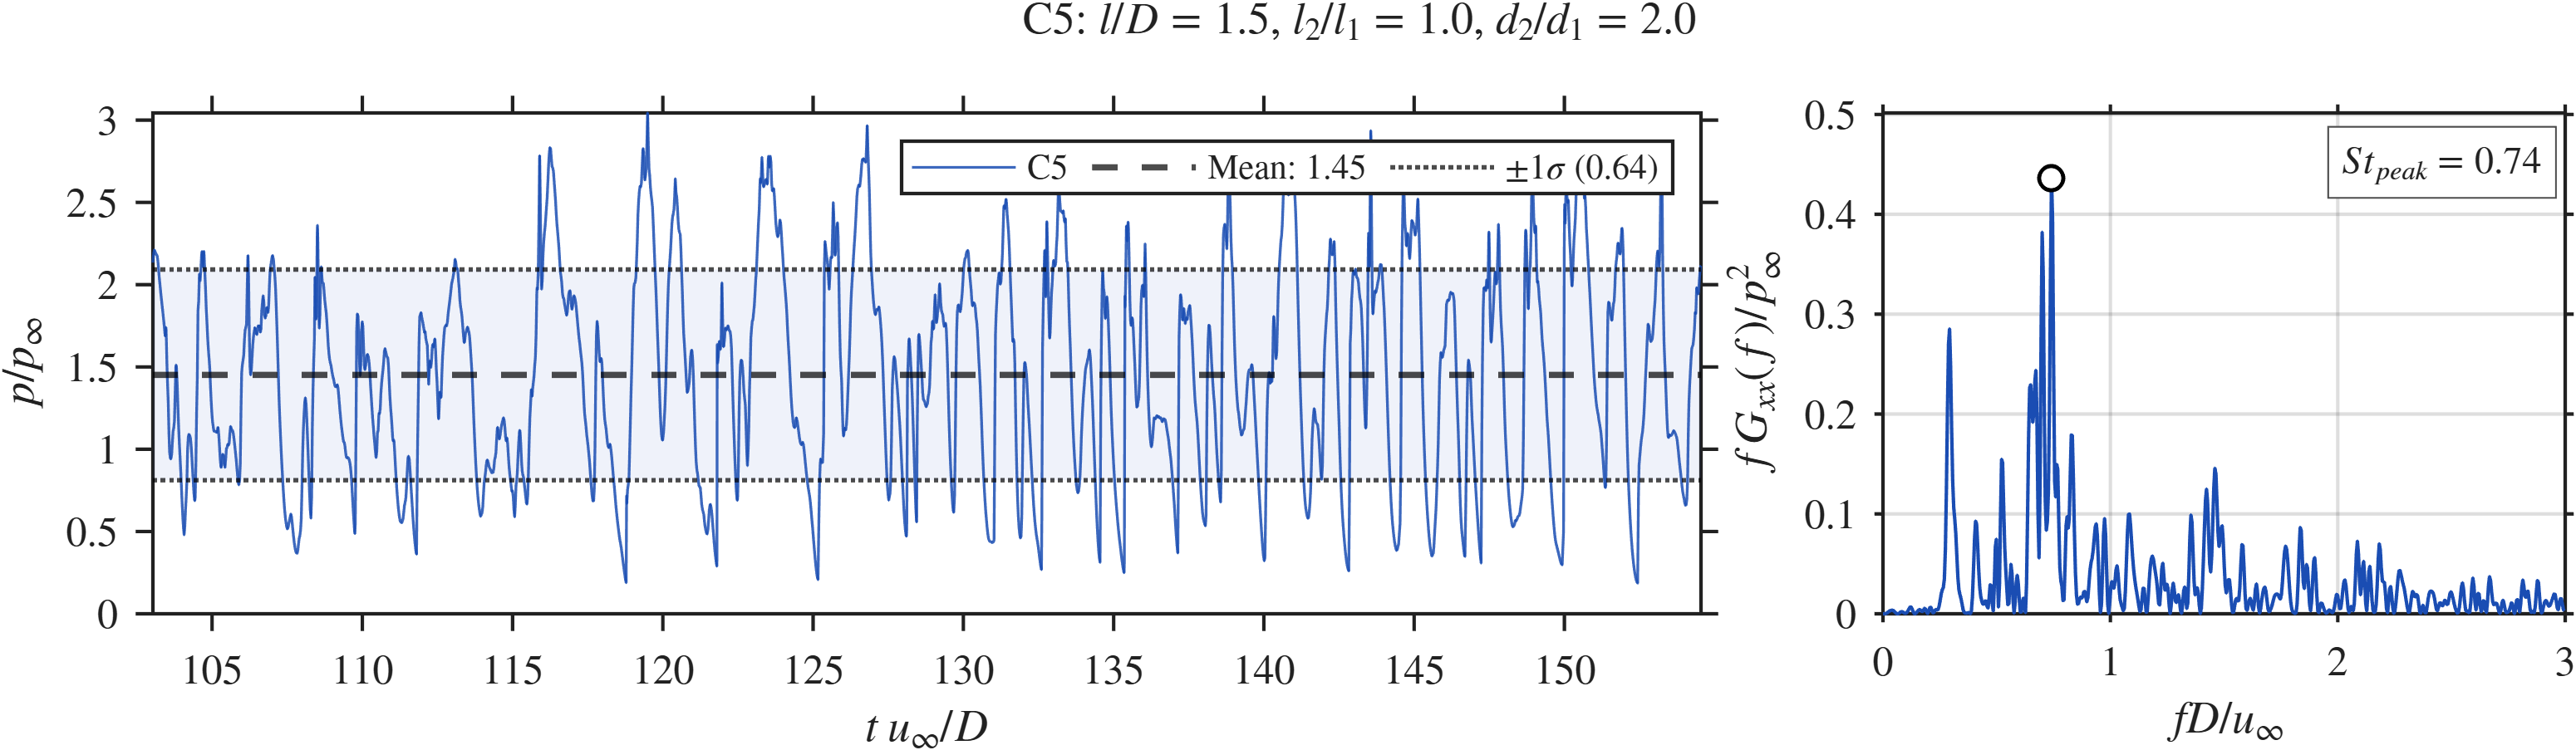
\includegraphics[width=\linewidth]{C5_psig.png}\caption{C5, pressure}\end{subfigure}\\
  \begin{subfigure}{\textwidth}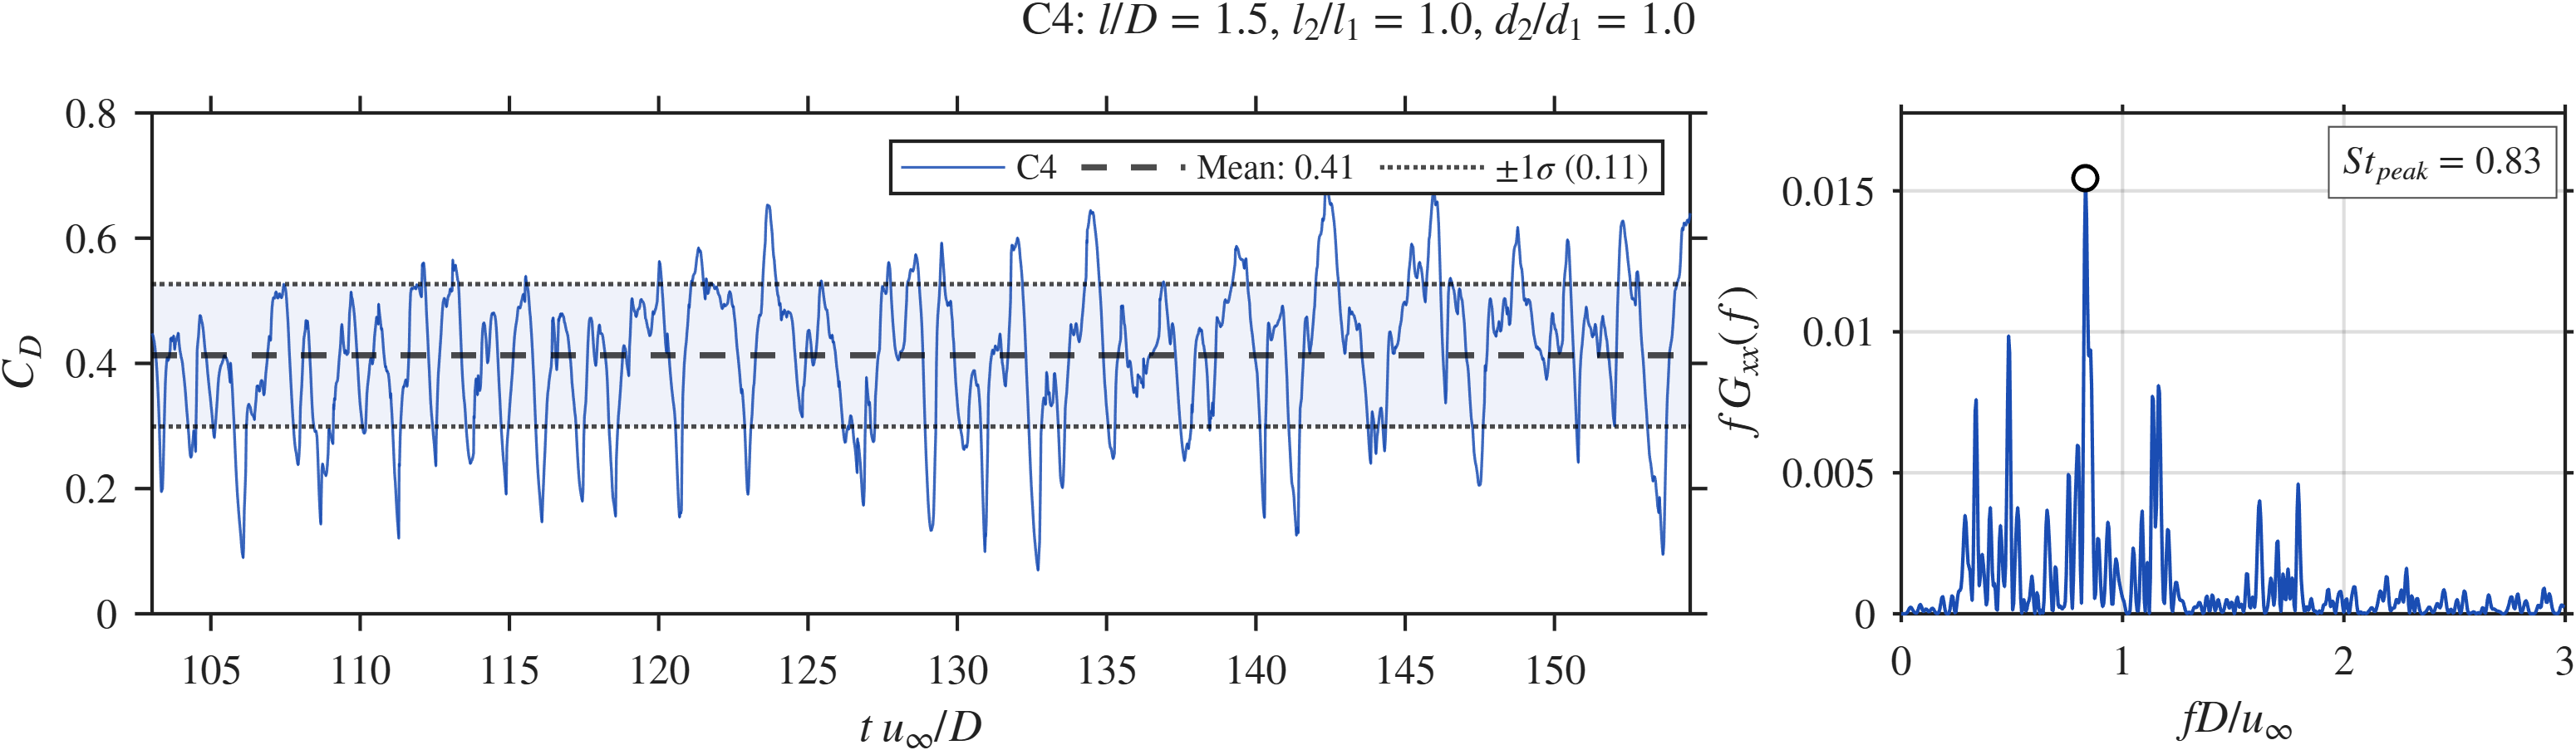
\includegraphics[width=\linewidth]{C4_dsig.png}\caption{C4, drag}\end{subfigure}\\
  \begin{subfigure}{\textwidth}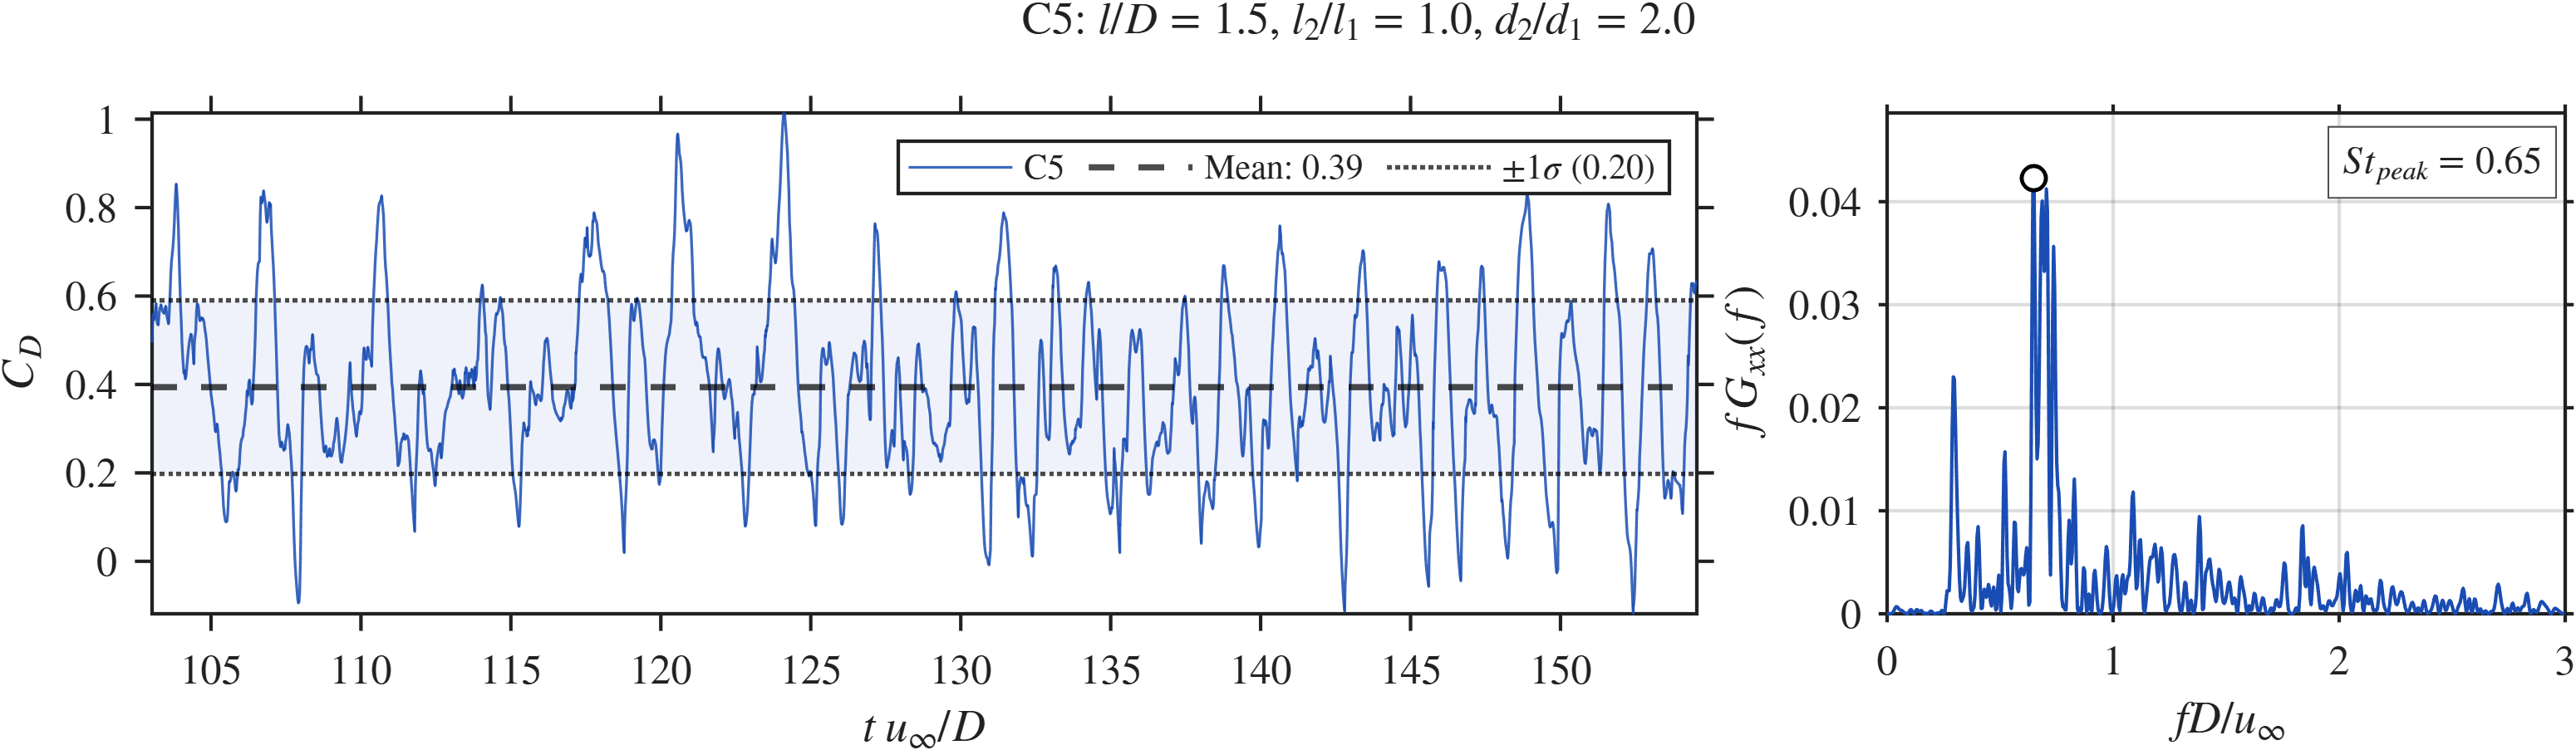
\includegraphics[width=\linewidth]{C5_dsig.png}\caption{C5, drag}\end{subfigure}
  \caption{Disk-diameter sweep: probe pressure and drag signals with spectra for C4 and C5.}
  \label{fig:dia_sig}
\end{figure}

\paragraph{SPOD.} Figure~\ref{fig:dia_spod} shows the SPOD results. C4 has its leading peak at $St = 0.835$ ($\lambda_1 \approx 1.4\times10^{-5}$), close to the SA tone, with a second peak of similar height at $St = 0.349$. Its leading mode runs continuously through both cavities to the shoulder, so the equal disk does not break the single feedback loop and the flow behaves like a single cavity with a small step in it. C5 has the highest peak of all eight cases ($\lambda_1 \approx 5.5\times10^{-5}$ at $St = 0.291$), the same frequency as the coupled mode of C1. Its leading mode sits in Cavity 1 and around the second disk, with weaker structures in Cavity 2. Its second peak at $St = 0.699$, near the SA tone, spans Cavity 2 and the shoulder, so the SA-type loop survives there as a weaker oscillation. The third peak at $St = 1.087$ is concentrated near the edge of the second disk. The second disk must be large enough ($\dtd \ge 1.5$) to intercept the shear layer and set up the two-cavity mode. At $\dtd = 1$ the SA-type single loop stays. At $\dtd = 2$ the second disk becomes a strong source of unsteadiness in its own right, which explains the high drag fluctuation.

\begin{figure}[htbp]
  \centering
  \begin{subfigure}{0.72\textwidth}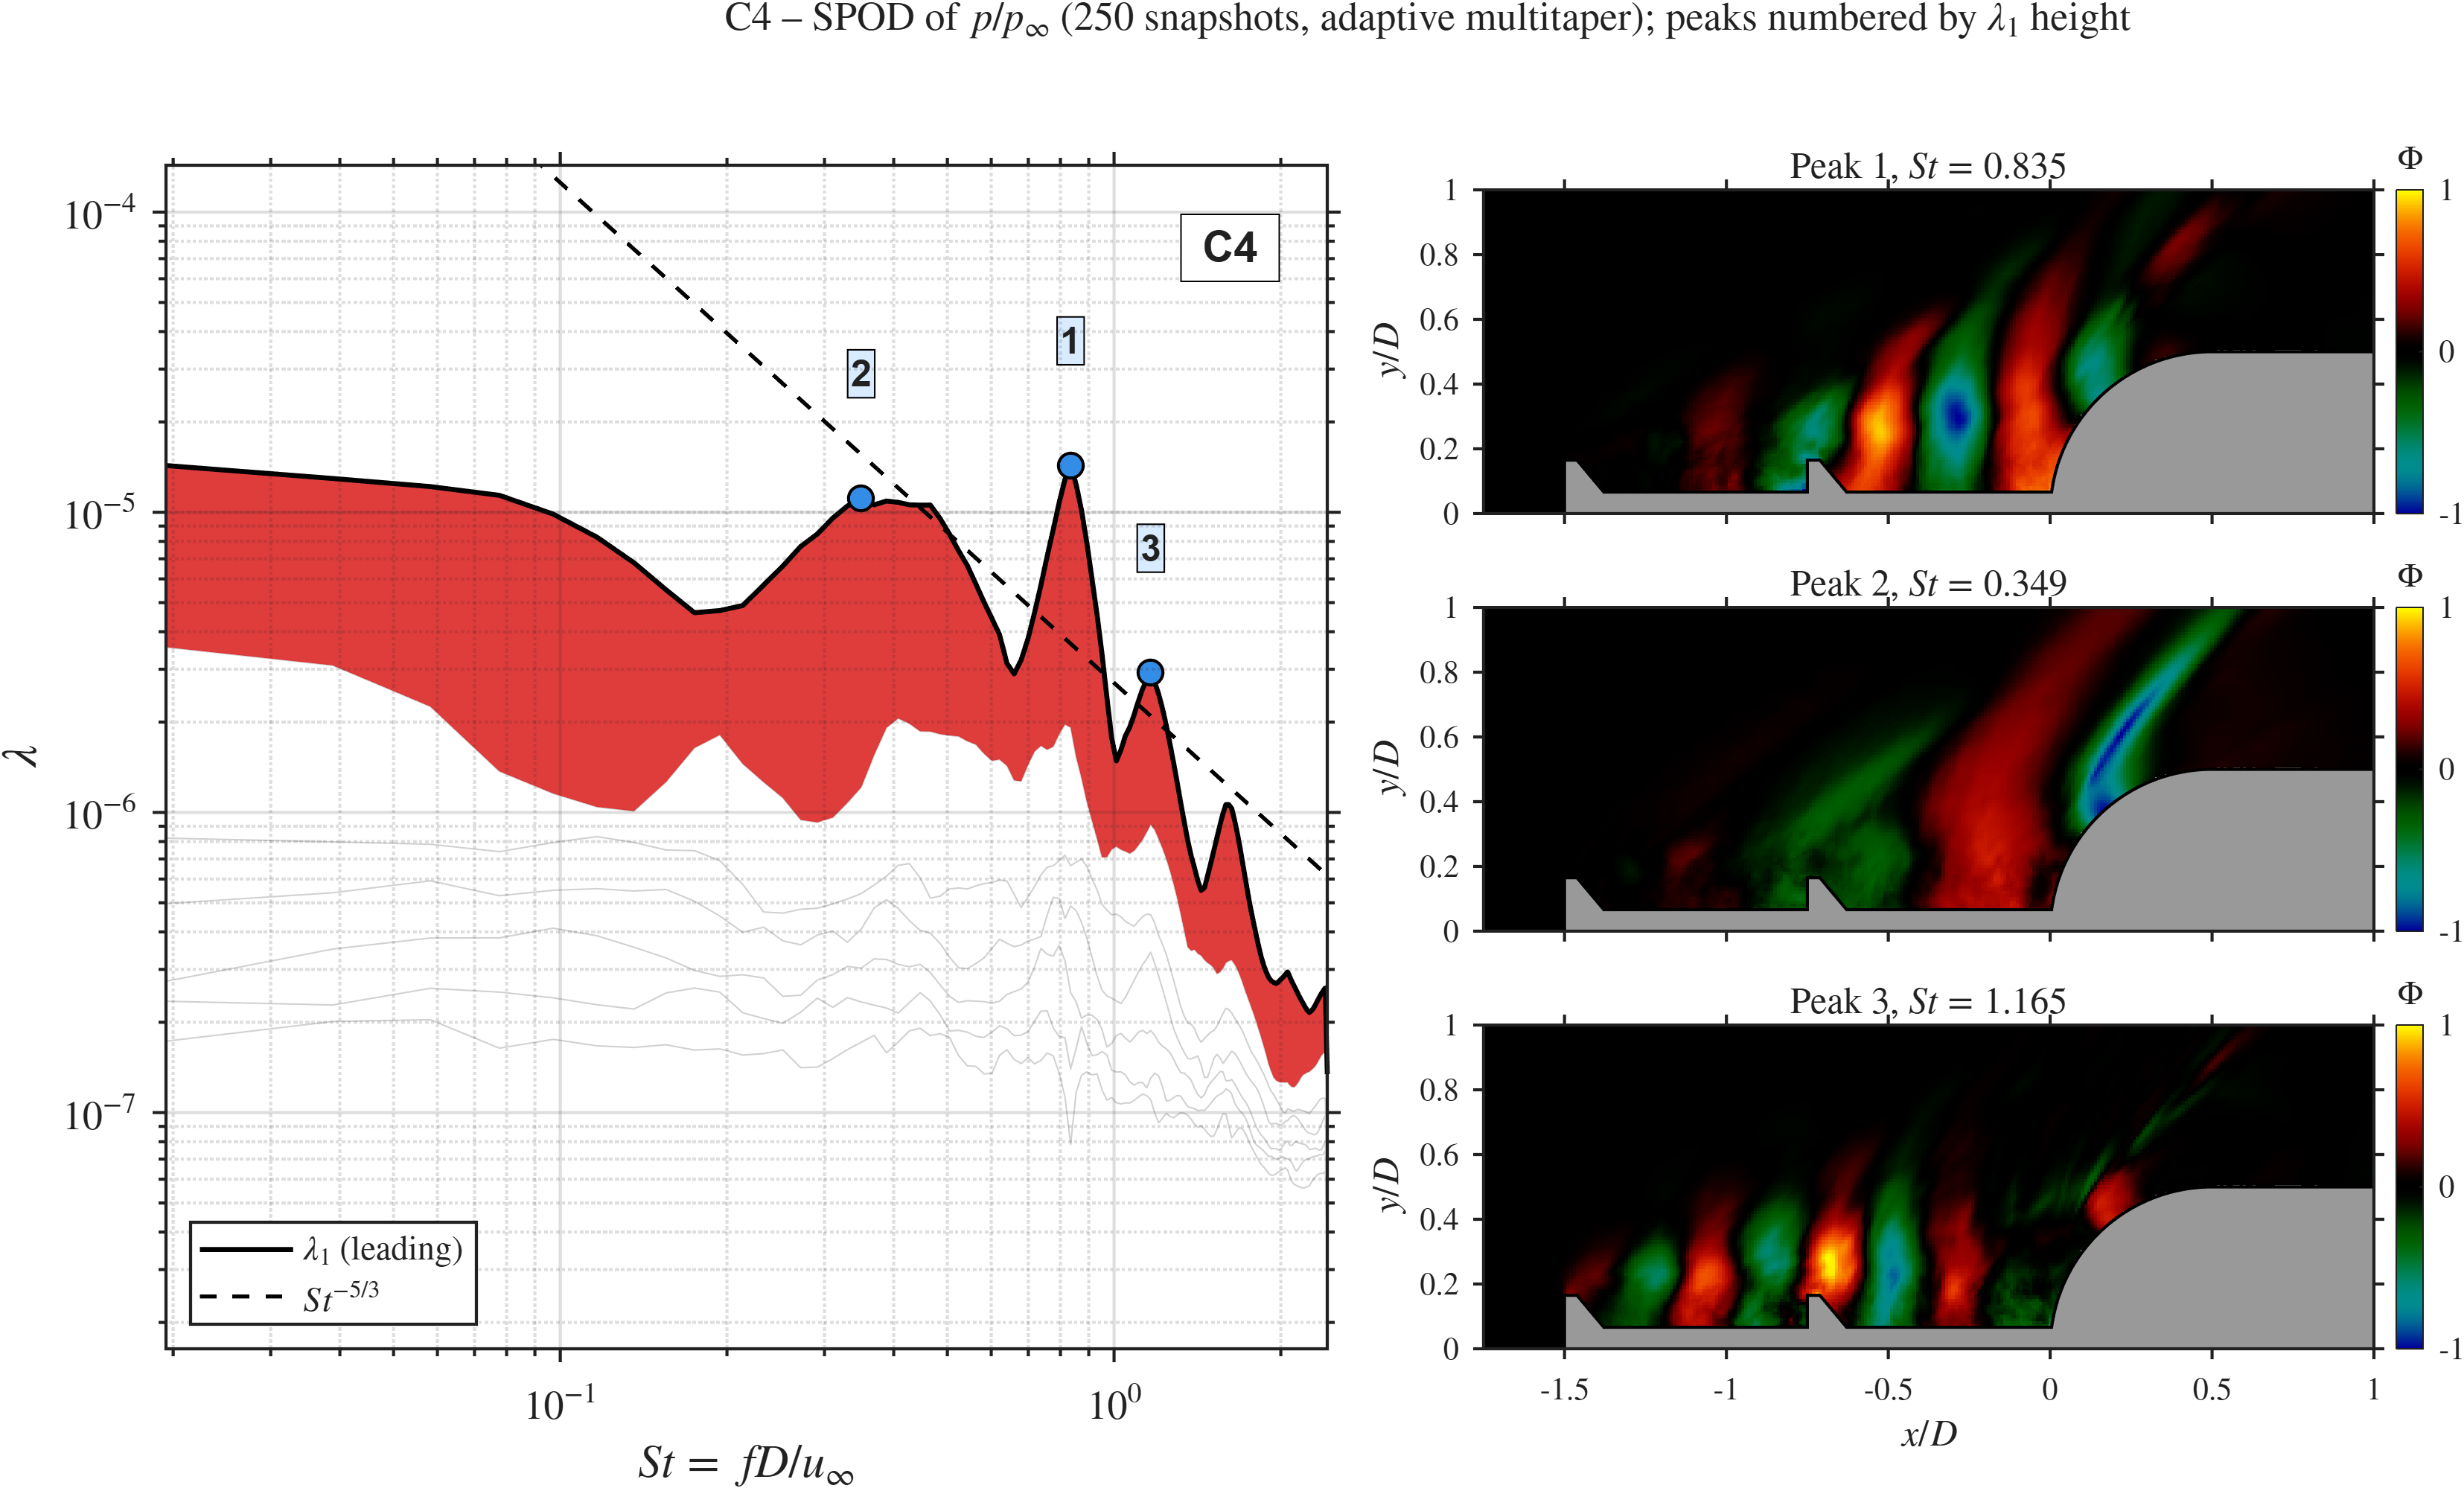
\includegraphics[width=\linewidth]{C4_spod.png}\caption{C4 ($\dtd = 1$)}\end{subfigure}\\
  \begin{subfigure}{0.72\textwidth}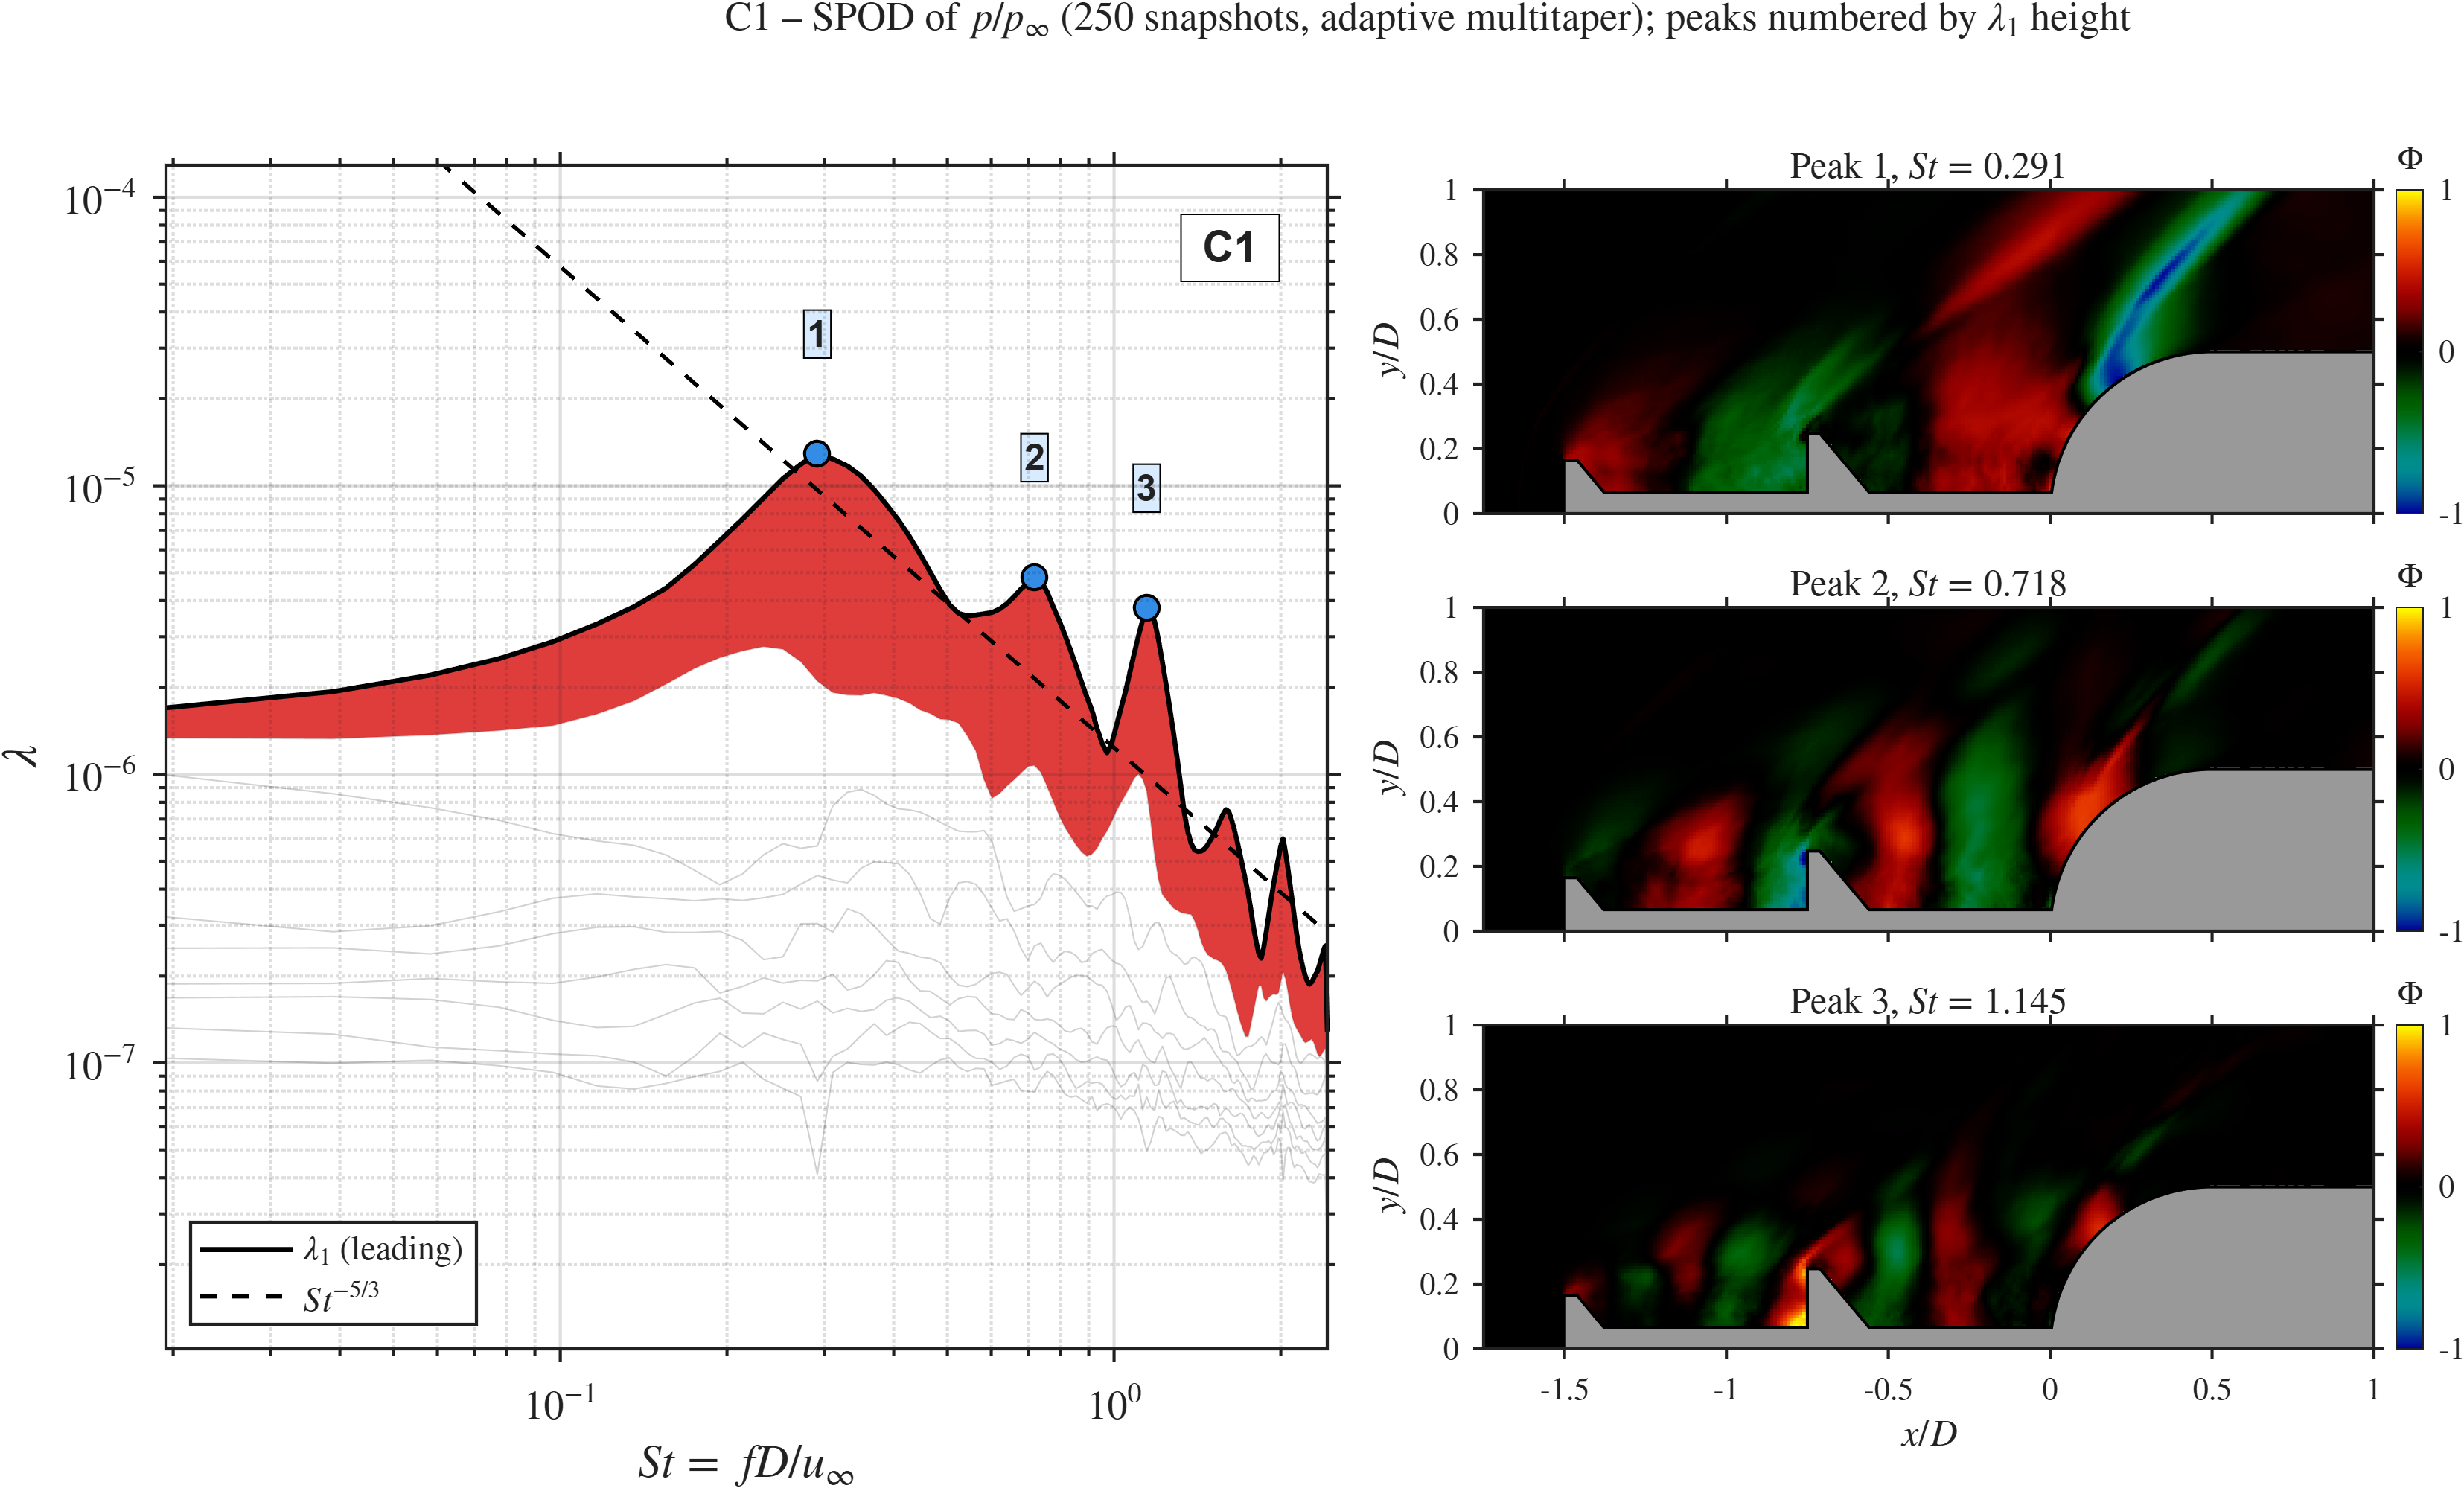
\includegraphics[width=\linewidth]{C1_spod.png}\caption{C1 ($\dtd = 1.5$)}\end{subfigure}\\
  \begin{subfigure}{0.72\textwidth}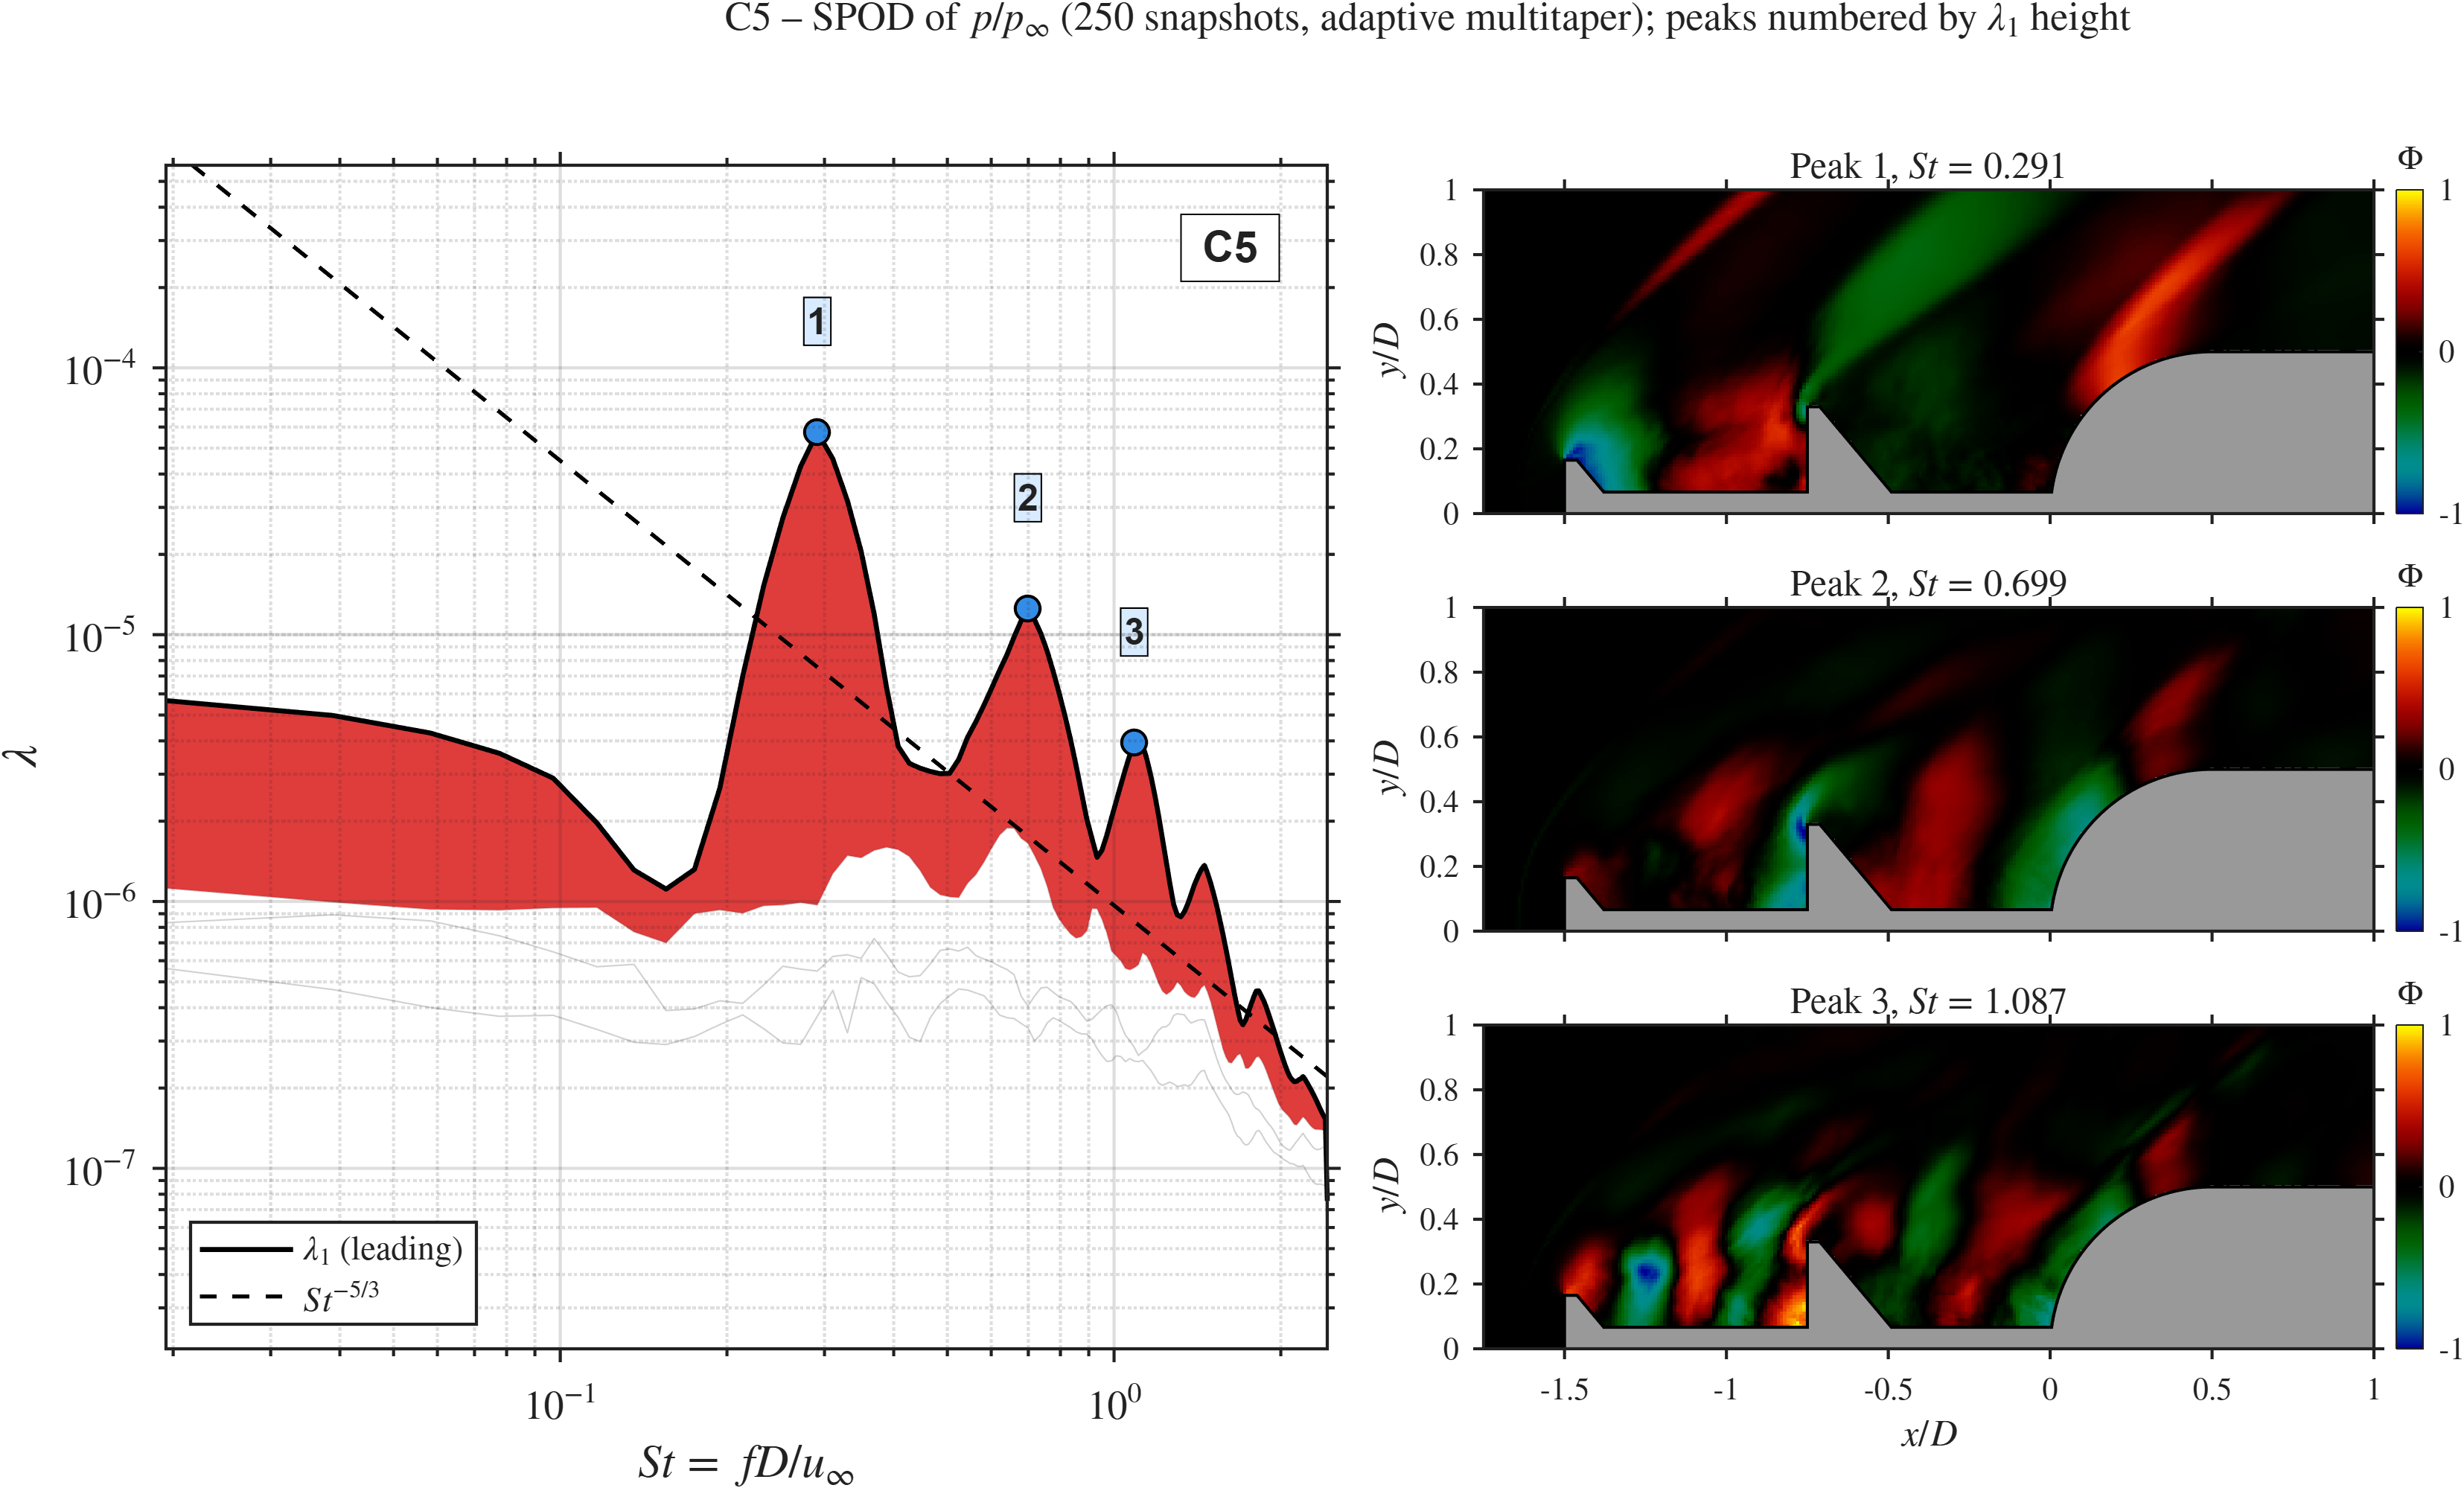
\includegraphics[width=\linewidth]{C5_spod.png}\caption{C5 ($\dtd = 2$)}\end{subfigure}
  \caption{Disk-diameter sweep: SPOD spectra and leading modes.}
  \label{fig:dia_spod}
\end{figure}

\paragraph{Summary.} Table~\ref{tab:dia} lists the trends. The disk diameter controls the mean shoulder pressure monotonically: $\pbar$ falls by 31.6\% from C4 (2.12) to C5 (1.45). The drag fluctuation moves the other way and rises by 82\% from C4 to C5. The equal-disk case C4 gives the highest mean pressure and fluctuation level of all cases and does not create the two-cavity mode, so a second disk the same size as the primary brings no benefit here. C1 ($\dtd = 1.5$) creates the two-cavity mode, has the broadest spectrum and keeps the drag fluctuation moderate. Our steady study found a change of regime near a radius ratio of 2~\cite{Gujar2026staged}, which is consistent with the jump in $\lambda_1$ and $\sCd$ seen here at $\dtd = 2$.

\begin{table}[htbp]
  \centering
  \caption{Disk-diameter sweep. Percentages are relative to the pivot C1.}
  \label{tab:dia}
  \begin{tabular}{lcccl}
    \toprule
    Metric & C4 ($\dtd = 1$) & C1 ($\dtd = 1.5$) & C5 ($\dtd = 2$) & Trend with $\dtd$ \\
    \midrule
    $\pbar$ & 2.12 ($+14.0\%$) & 1.86 & 1.45 ($-22.0\%$) & falls \\
    $\psd$ & 0.87 ($+19.2\%$) & 0.73 & 0.64 ($-12.3\%$) & falls \\
    $\Cdm$ & 0.41 ($+5.1\%$) & 0.39 & 0.39 (0\%) & weak \\
    $\sCd$ & 0.11 ($-8.3\%$) & 0.12 & 0.20 ($+66.7\%$) & rises \\
    $St$ peak, pressure & 0.83 & 1.12 & 0.74 & non-monotonic \\
    $St$ peak, drag & 0.83 & 1.14 & 0.65 & non-monotonic \\
    Peak $\Pi$ & $\approx 0.72$ & $\approx 0.37$ & $\approx 0.44$ & non-monotonic \\
    SPOD leading $St$ & 0.835 & 0.291 & 0.291 & step at $\dtd \ge 1.5$ \\
    SPOD peak $\lambda_1$ & $\approx 1.4\times10^{-5}$ & $\approx 1.3\times10^{-5}$ & $\approx 5.5\times10^{-5}$ & jump at $\dtd = 2$ \\
    \bottomrule
  \end{tabular}
\end{table}

% ------------------------------------------------------------
\subsection{Effect of the spike length $l/D$ (C6, C1, C7)}\label{sec:len}

This sweep changes the total spike length at fixed $\dtd = 1.5$ and $\ltl = 1$, so the two cavities stay equal ($l_1 = l_2 = l/2$) (RQ4). The spike tip sits at $x/D = -1.0$ (C6), $-1.5$ (C1) and $-2.0$ (C7), and the second disk at $x/D = -0.5$, $-0.75$ and $-1.0$.

\paragraph{Mean flow and fluctuations.} Figure~\ref{fig:len_ms} shows the contours. In C6 ($l/D = 1$) both disks lie within one diameter of the hemisphere. The shear layer has little distance to grow before it reaches the body, both recirculation cells are small, and the bow shock sits close to the forebody. The shoulder pressure is the highest of this sweep ($\pbar = 2.03$). In C7 ($l/D = 2$) both cavities are $1.0D$ long and hold large low-pressure regions ($\pbar < 0.4$). The shoulder pressure drops to 1.83, 10\% below C6, as the longer shear layer weakens the reattachment shock. The fluctuations show the cost of the longer spike. In C6 the strong region ($\psd > 0.6$) is a narrow band between the second disk and the shoulder, and the flow ahead of the primary disk is almost steady. In C7 the band with $\psd > 0.4$ runs from $x/D \approx -1.5$ through Cavity 2 to the shoulder, about $2D$ long, and the probe value ($\psd = 0.83$) is the second highest of all cases after C4. The longer shear layer gives the vortices more distance to grow and feeds more unsteady energy into both cavities.

\begin{figure}[htbp]
  \centering
  \begin{subfigure}{0.49\textwidth}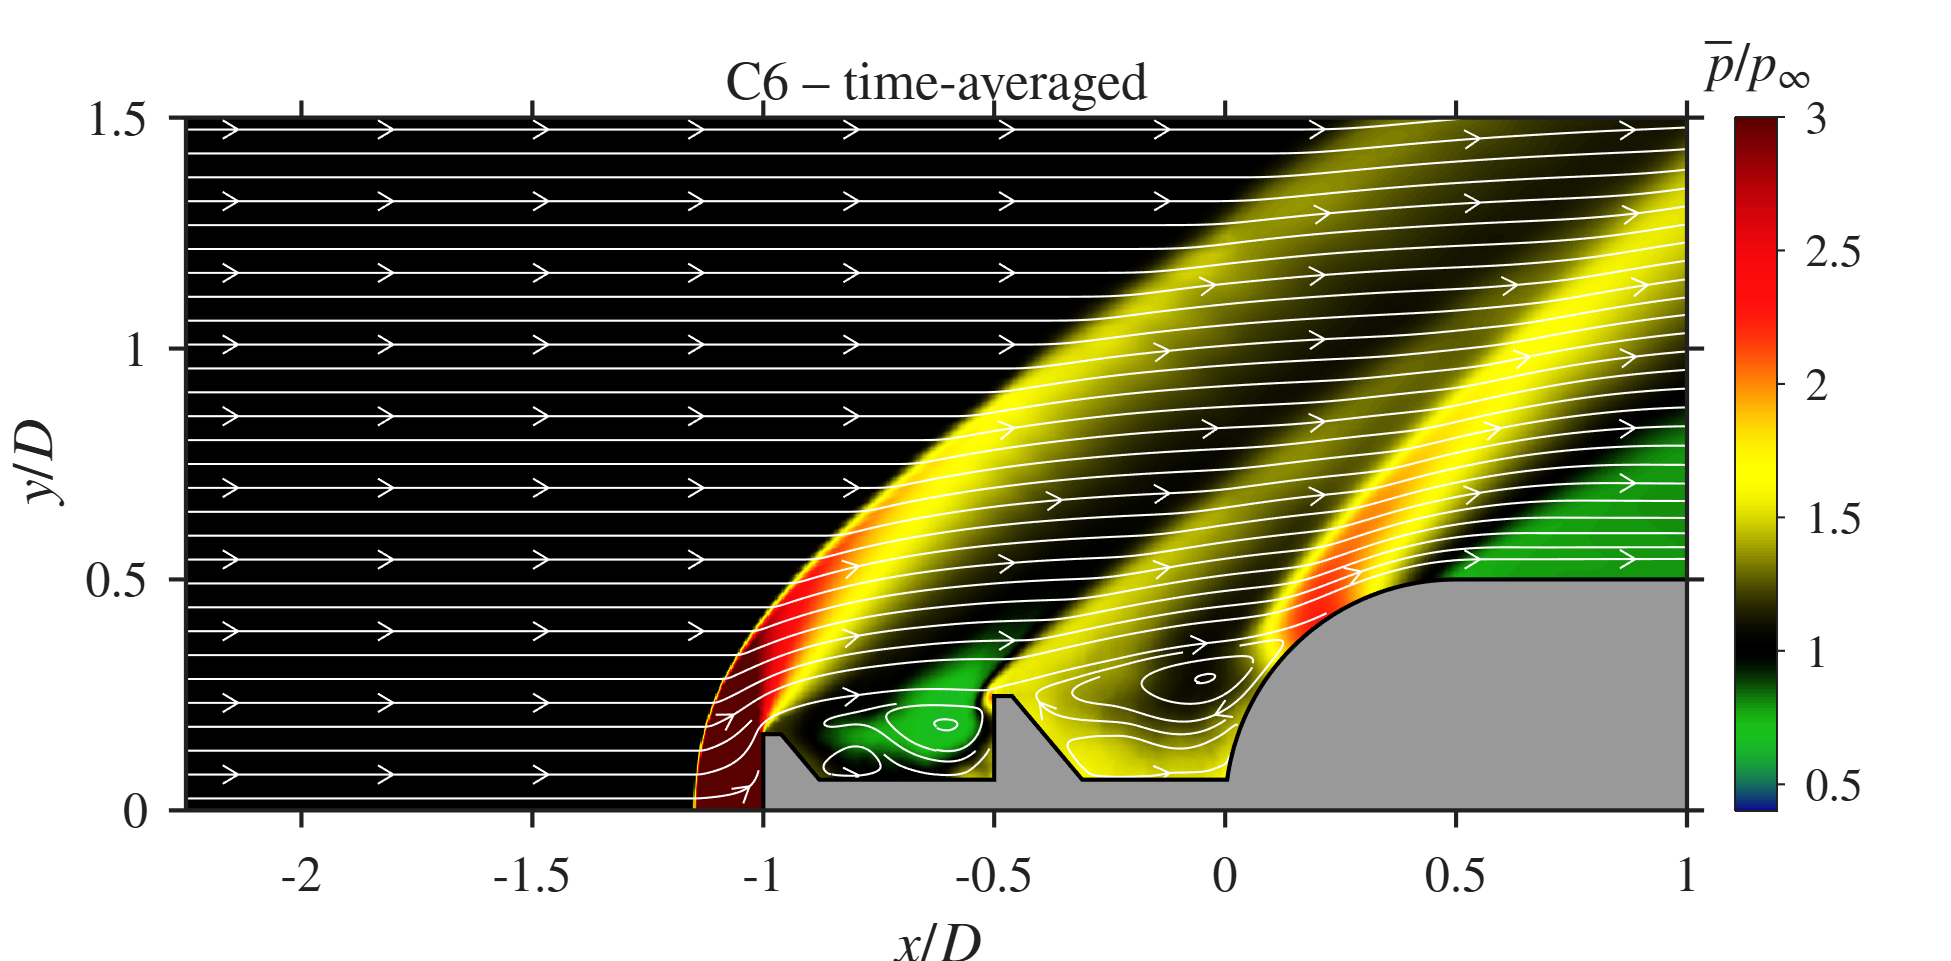
\includegraphics[width=\linewidth]{C6_mean.png}\caption{C6 ($l/D = 1$), $\pbar$}\end{subfigure}
  \begin{subfigure}{0.49\textwidth}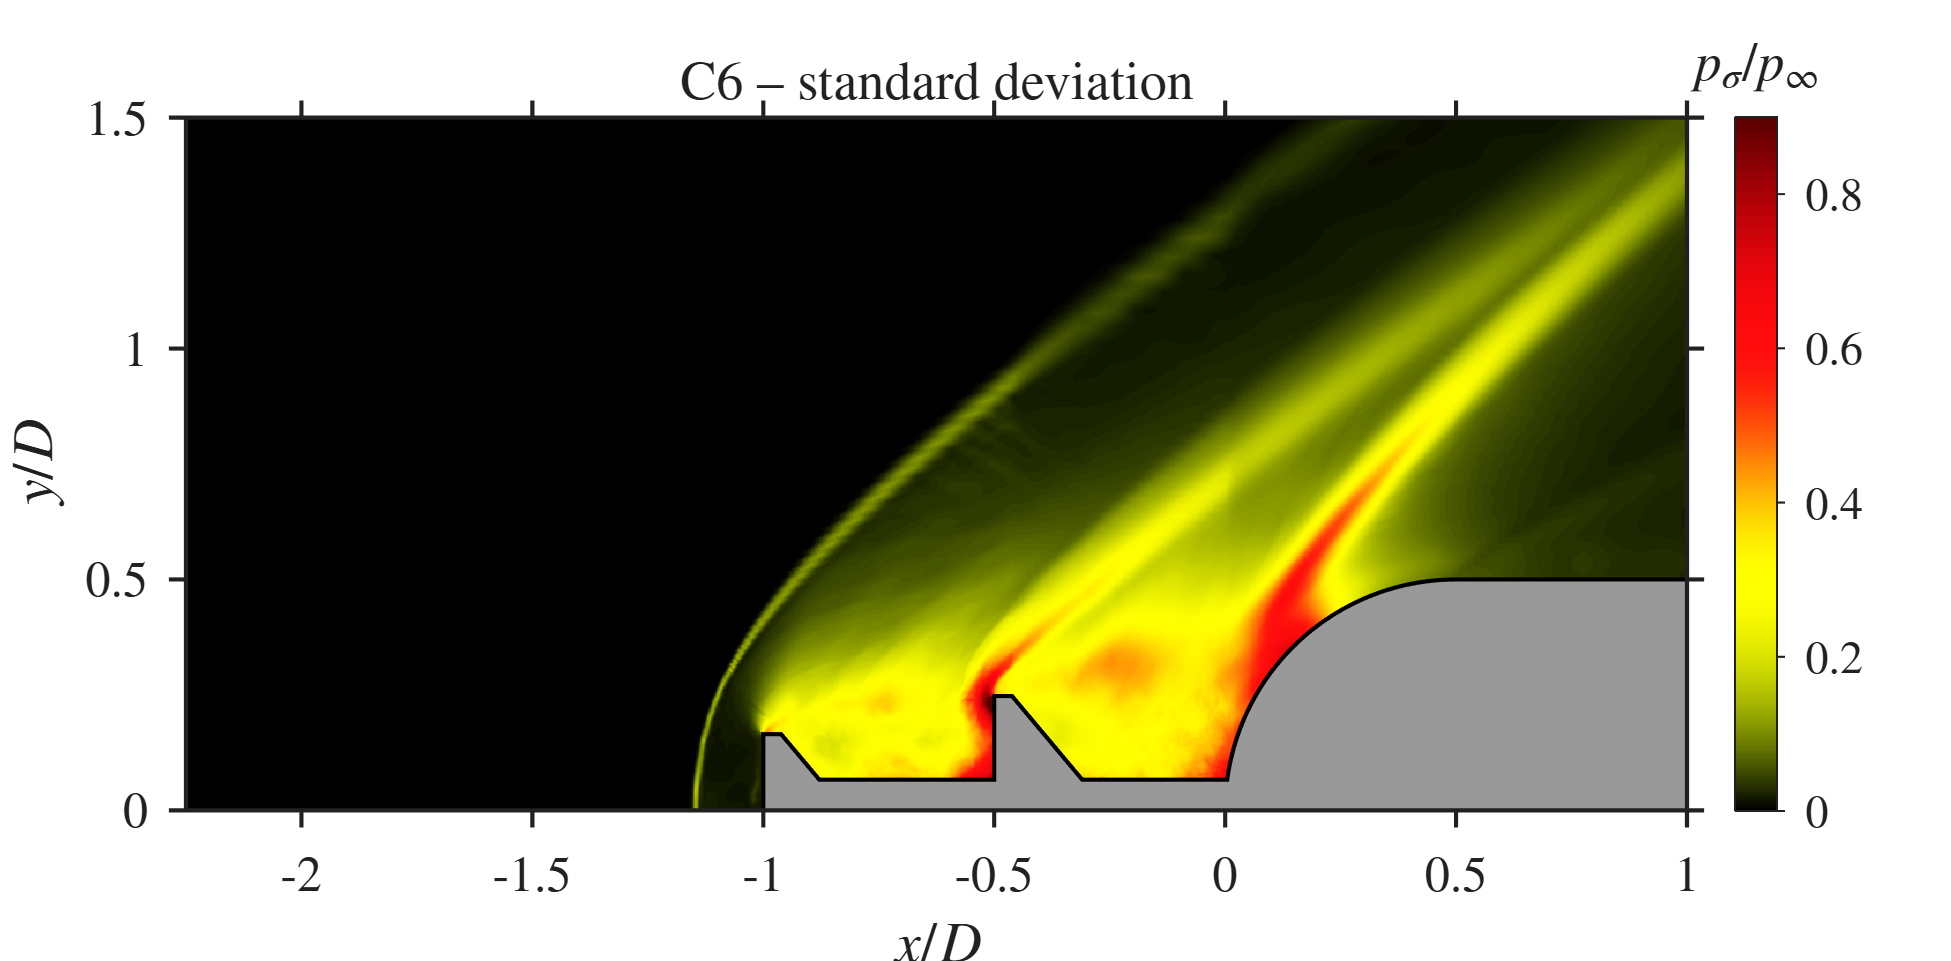
\includegraphics[width=\linewidth]{C6_std.png}\caption{C6, $\psd$}\end{subfigure}\\[2pt]
  \begin{subfigure}{0.49\textwidth}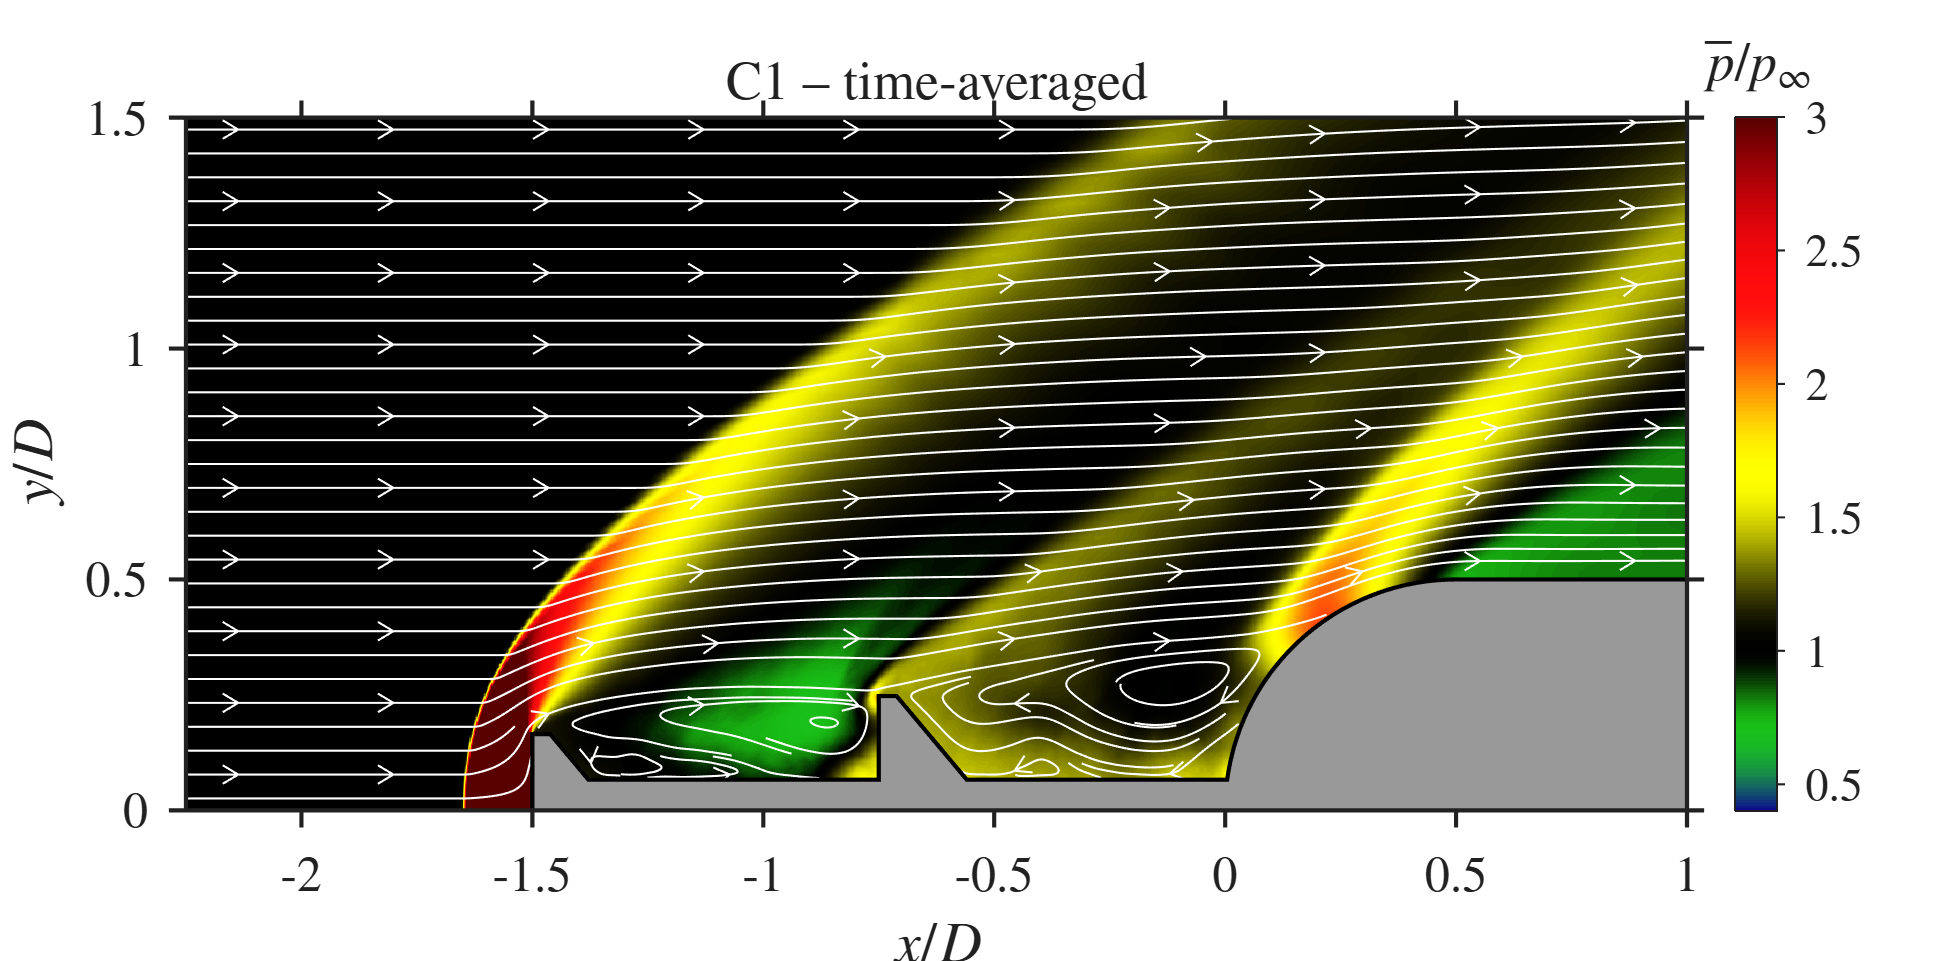
\includegraphics[width=\linewidth]{C1_mean.png}\caption{C1 ($l/D = 1.5$), $\pbar$}\end{subfigure}
  \begin{subfigure}{0.49\textwidth}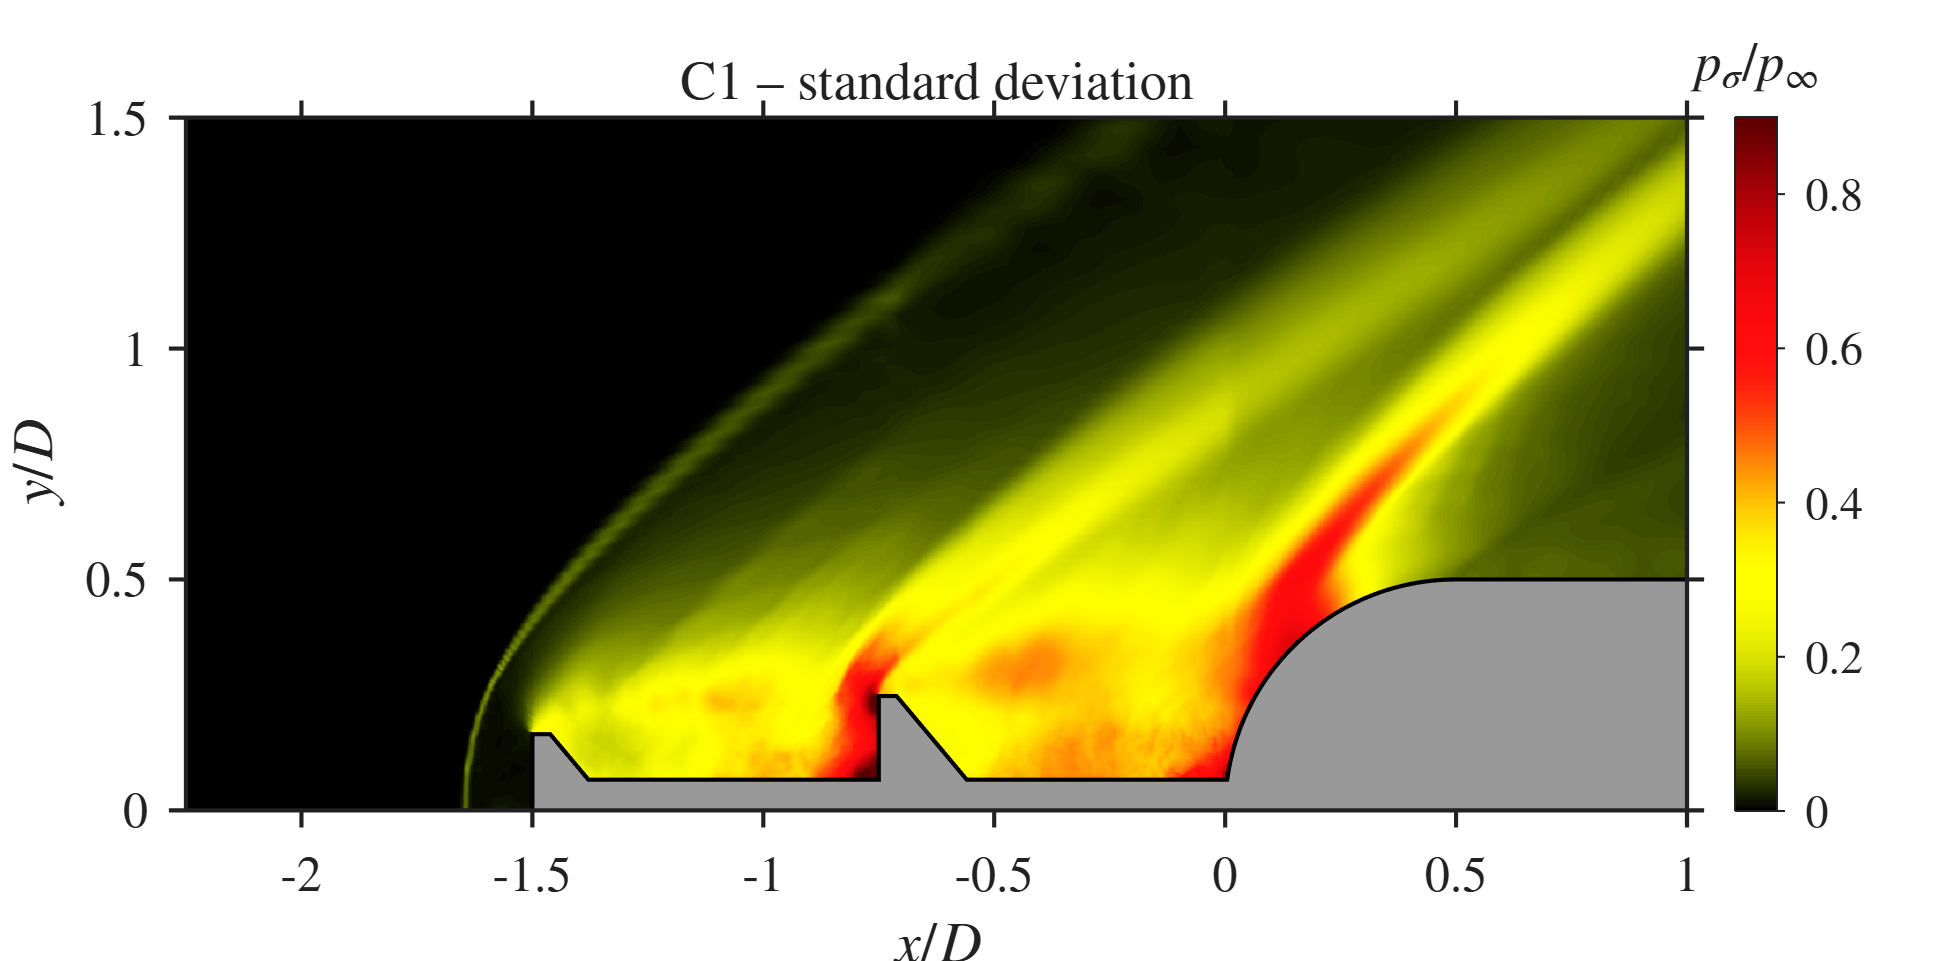
\includegraphics[width=\linewidth]{C1_std.png}\caption{C1, $\psd$}\end{subfigure}\\[2pt]
  \begin{subfigure}{0.49\textwidth}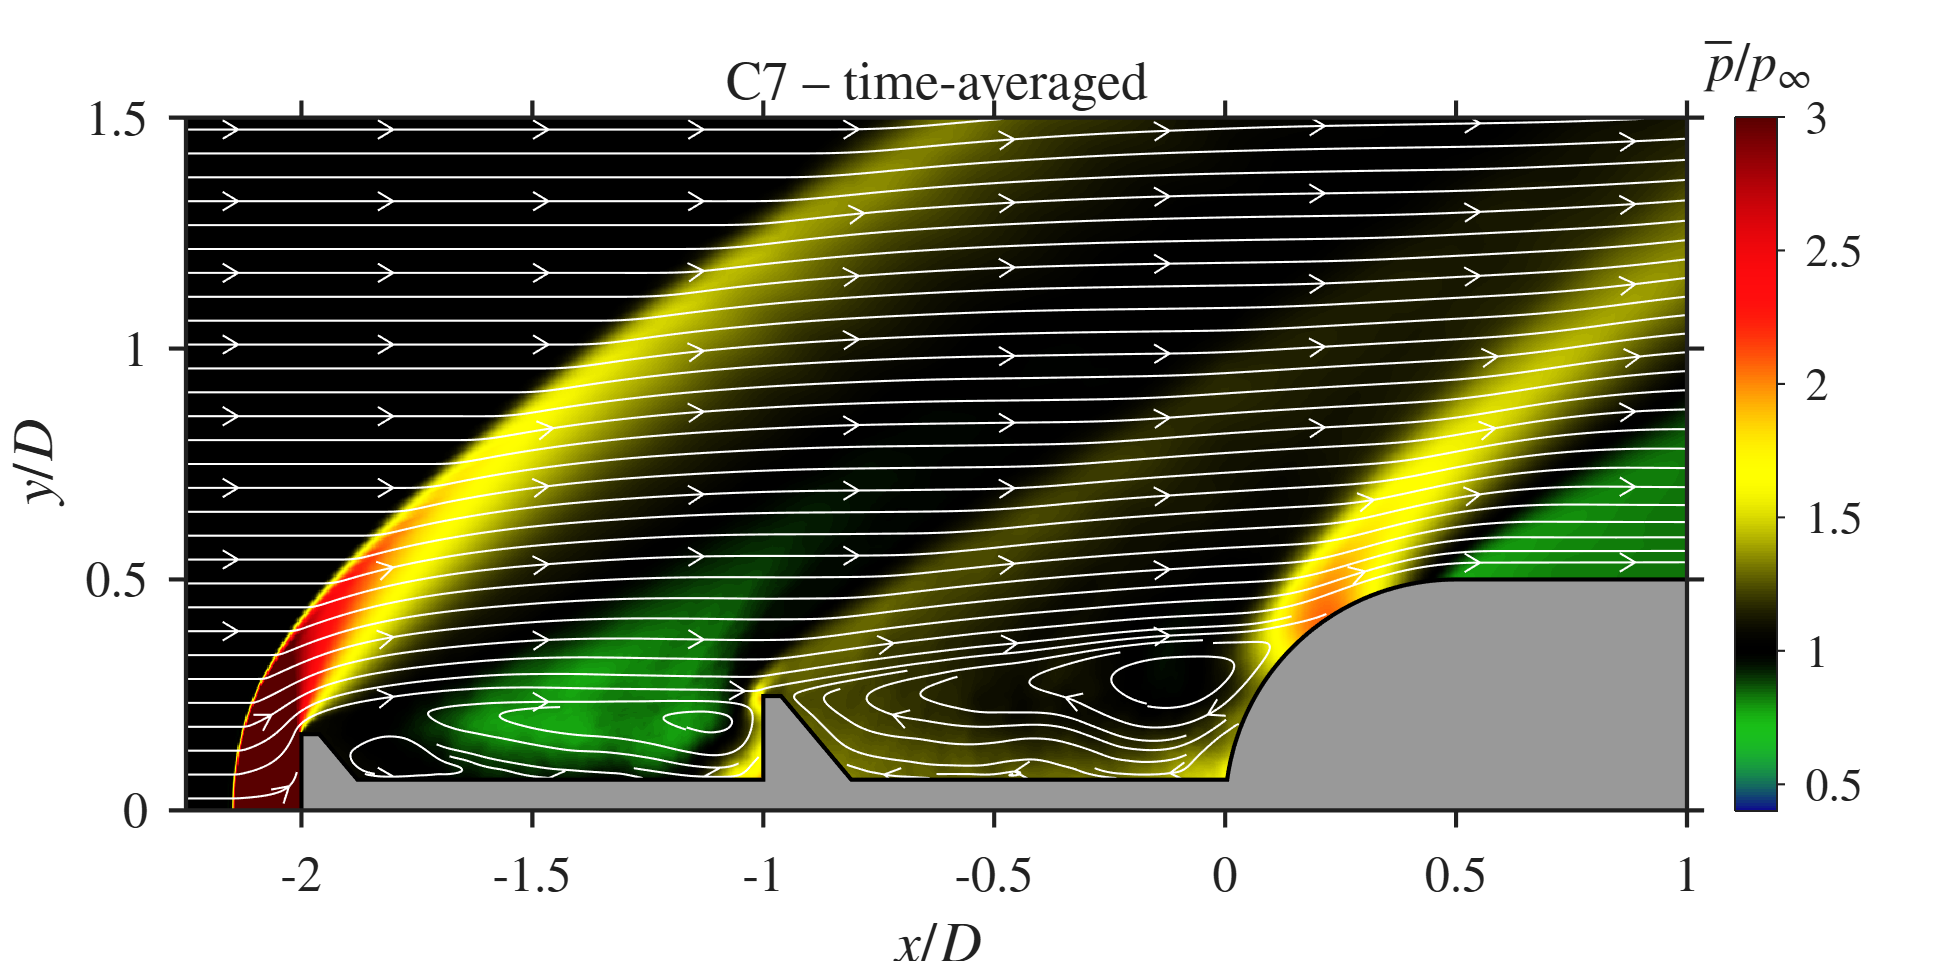
\includegraphics[width=\linewidth]{C7_mean.png}\caption{C7 ($l/D = 2$), $\pbar$}\end{subfigure}
  \begin{subfigure}{0.49\textwidth}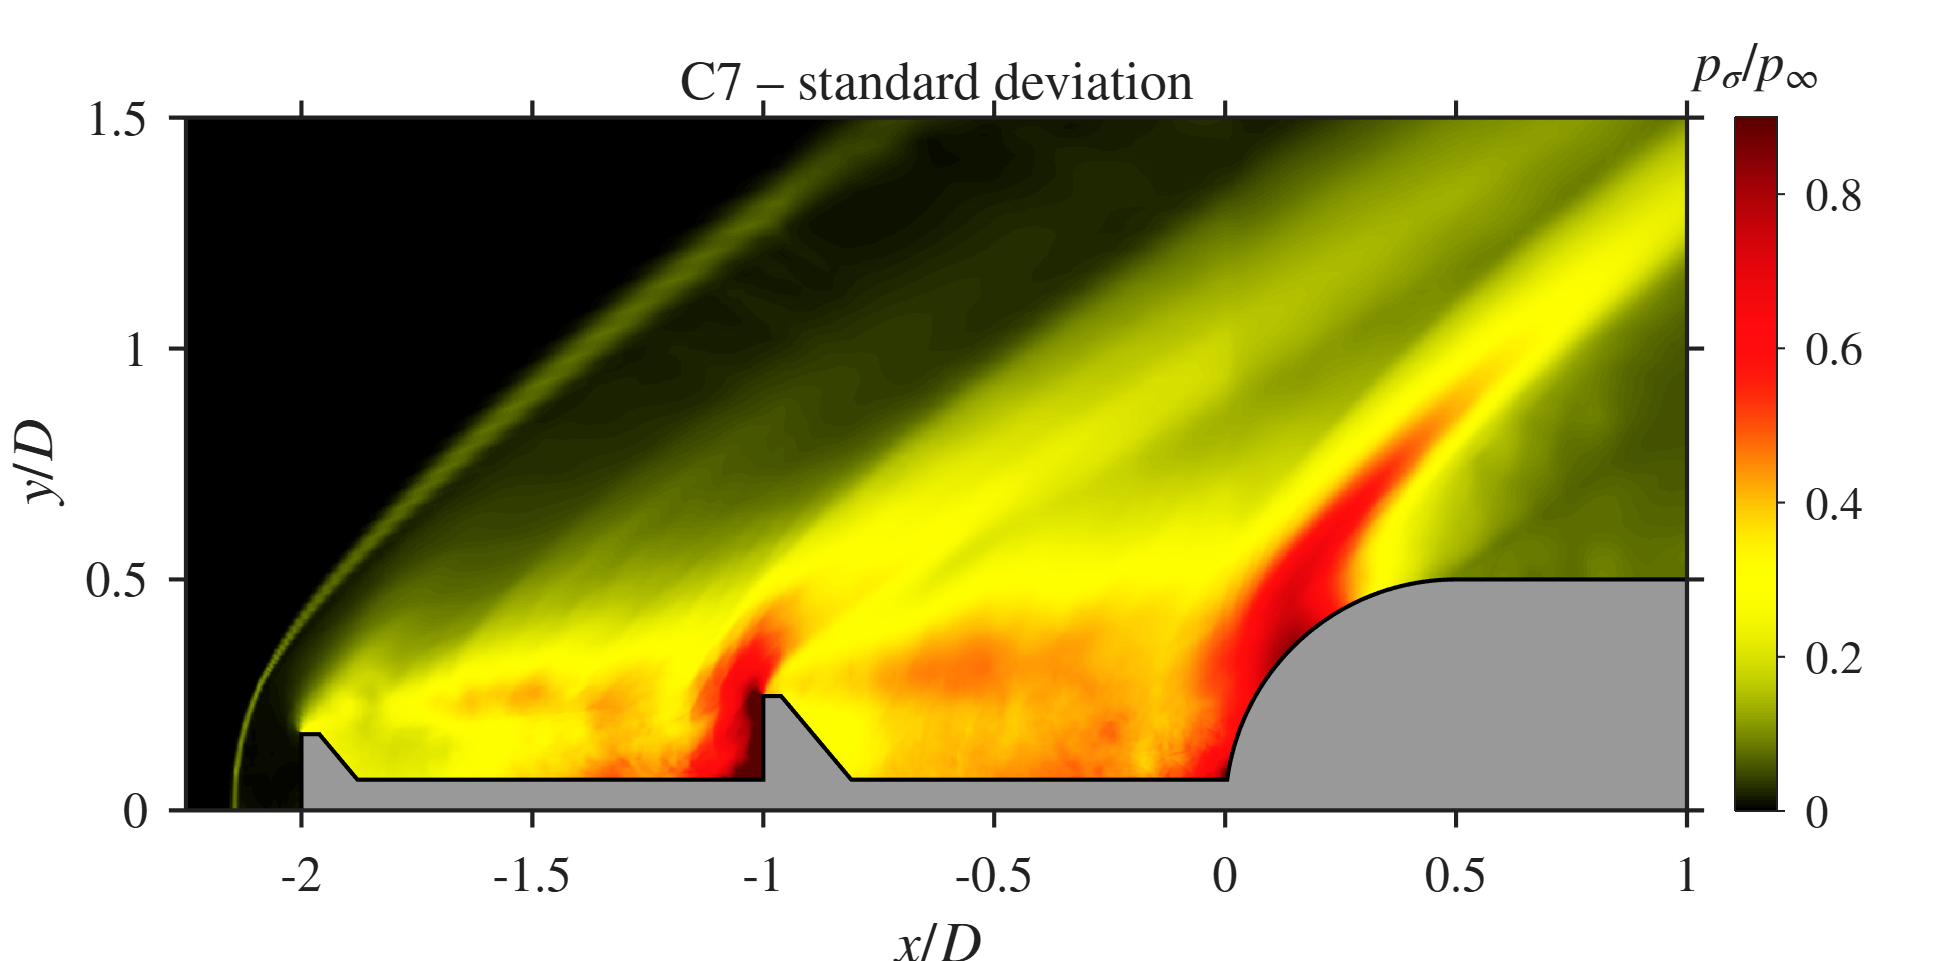
\includegraphics[width=\linewidth]{C7_std.png}\caption{C7, $\psd$}\end{subfigure}
  \caption{Spike-length sweep: mean pressure with streamlines (left) and pressure standard deviation (right).}
  \label{fig:len_ms}
\end{figure}

\paragraph{Space-time behaviour.} Figures~\ref{fig:len_xt} and~\ref{fig:len_xf} show the $x$--$t$ and $x$--$f$ diagrams. In C6 both cavities share one band at $St \approx 1.13$, the same as the probe and drag peaks. In C7 the disk-face band sits at $St \approx 1.16$ and Cavity 2 carries $St \approx 0.89$. The disk-face band stays near $St \approx 1.1$ to 1.2 in C1, C2, C4, C6 and C7 even though $l_1$ changes from $0.5D$ to $1.0D$ across these cases \chk{CHECK: worth a short discussion of what sets this frequency}.

\begin{figure}[htbp]
  \centering
  \begin{subfigure}{0.325\textwidth}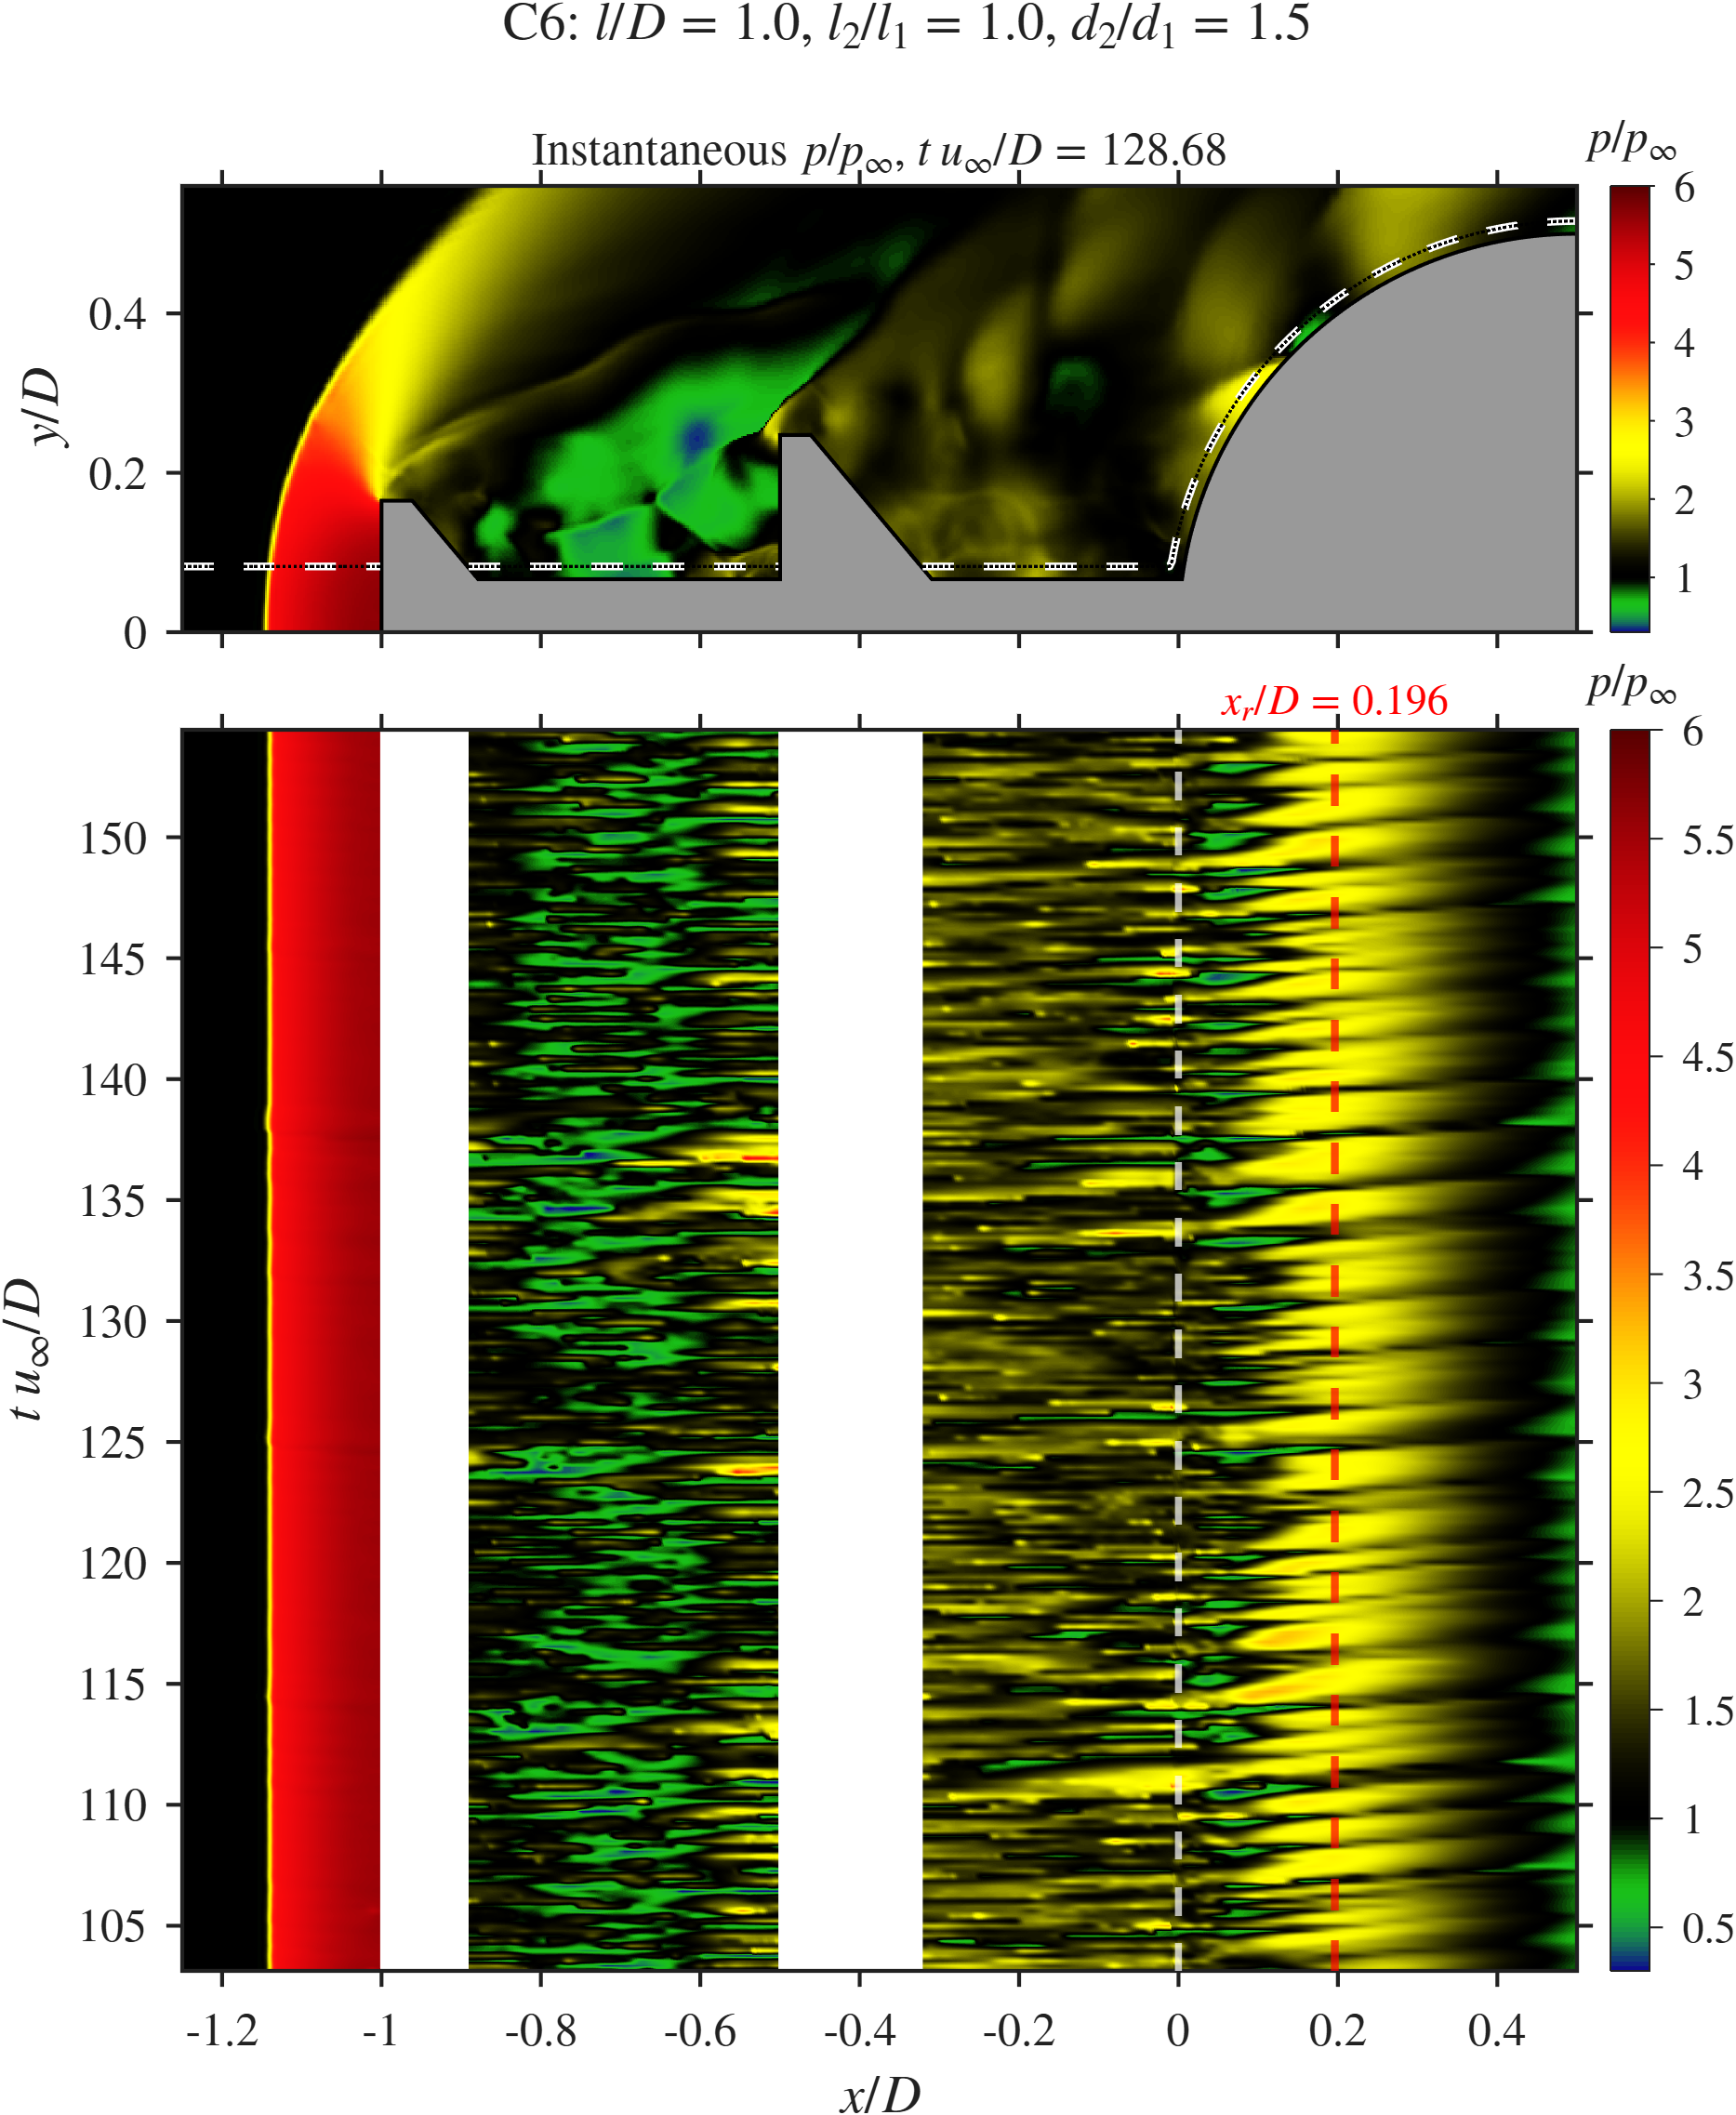
\includegraphics[width=\linewidth]{C6_xt.png}\caption{C6}\end{subfigure}
  \begin{subfigure}{0.325\textwidth}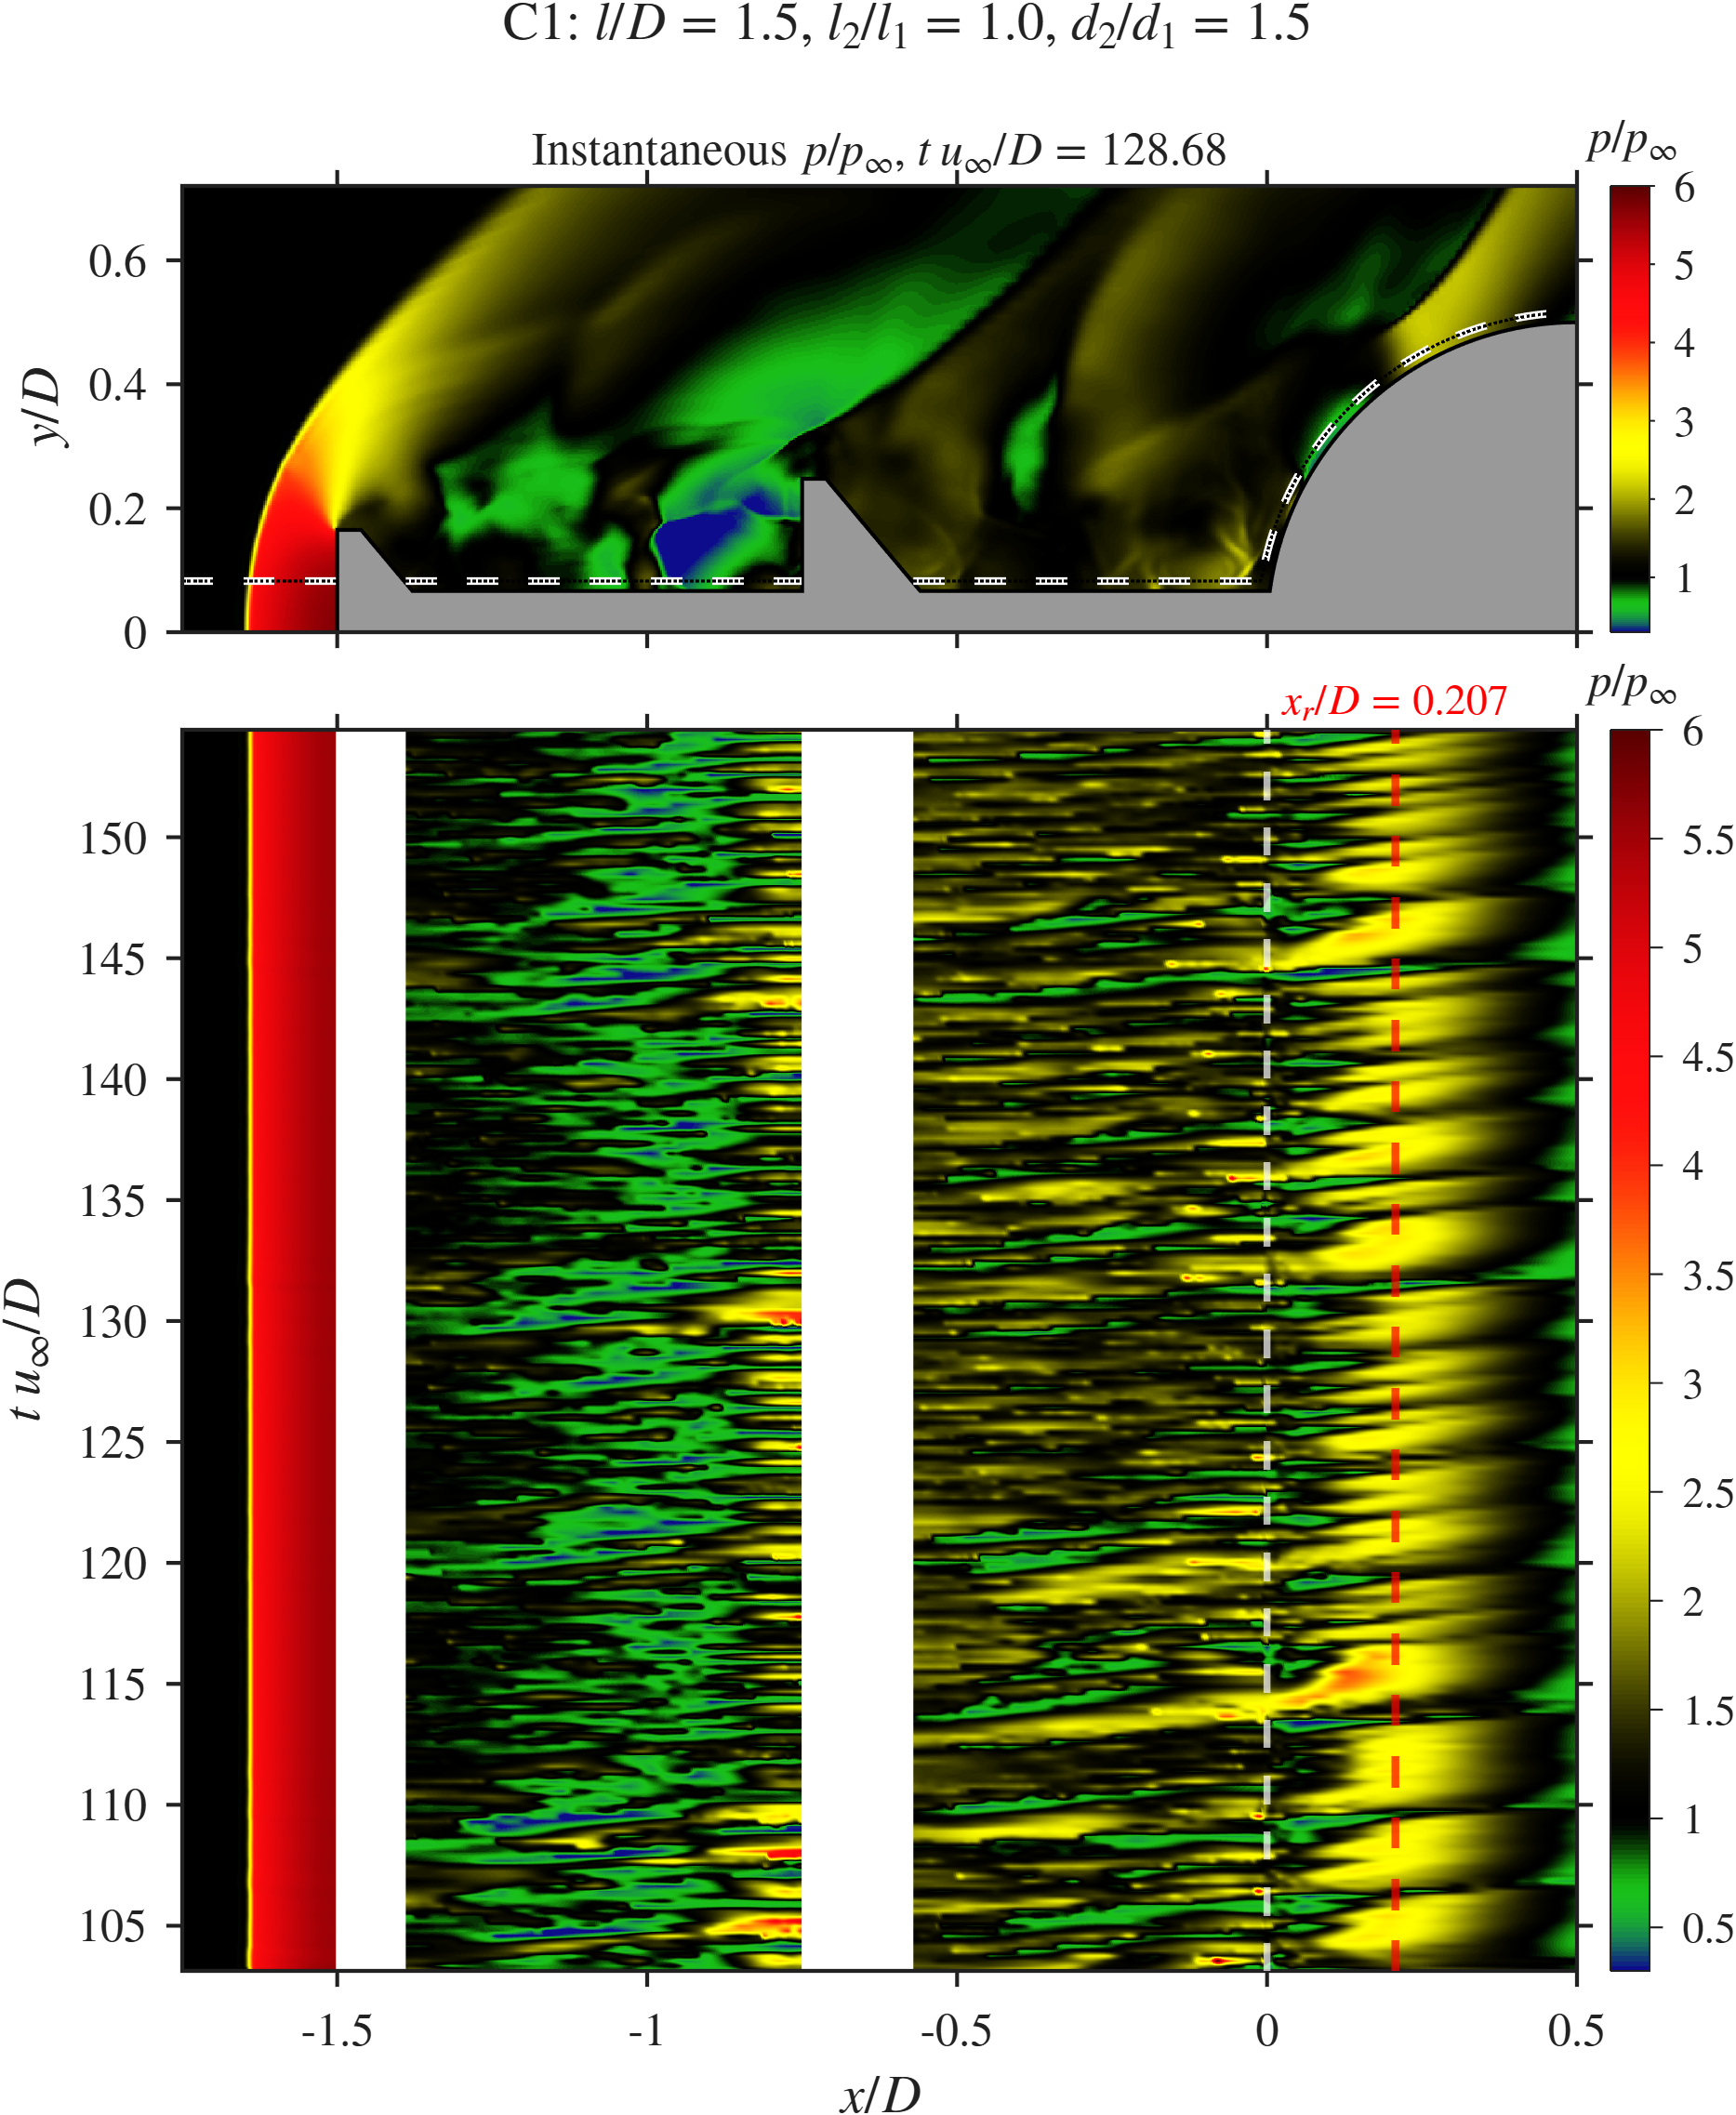
\includegraphics[width=\linewidth]{C1_xt.png}\caption{C1}\end{subfigure}
  \begin{subfigure}{0.325\textwidth}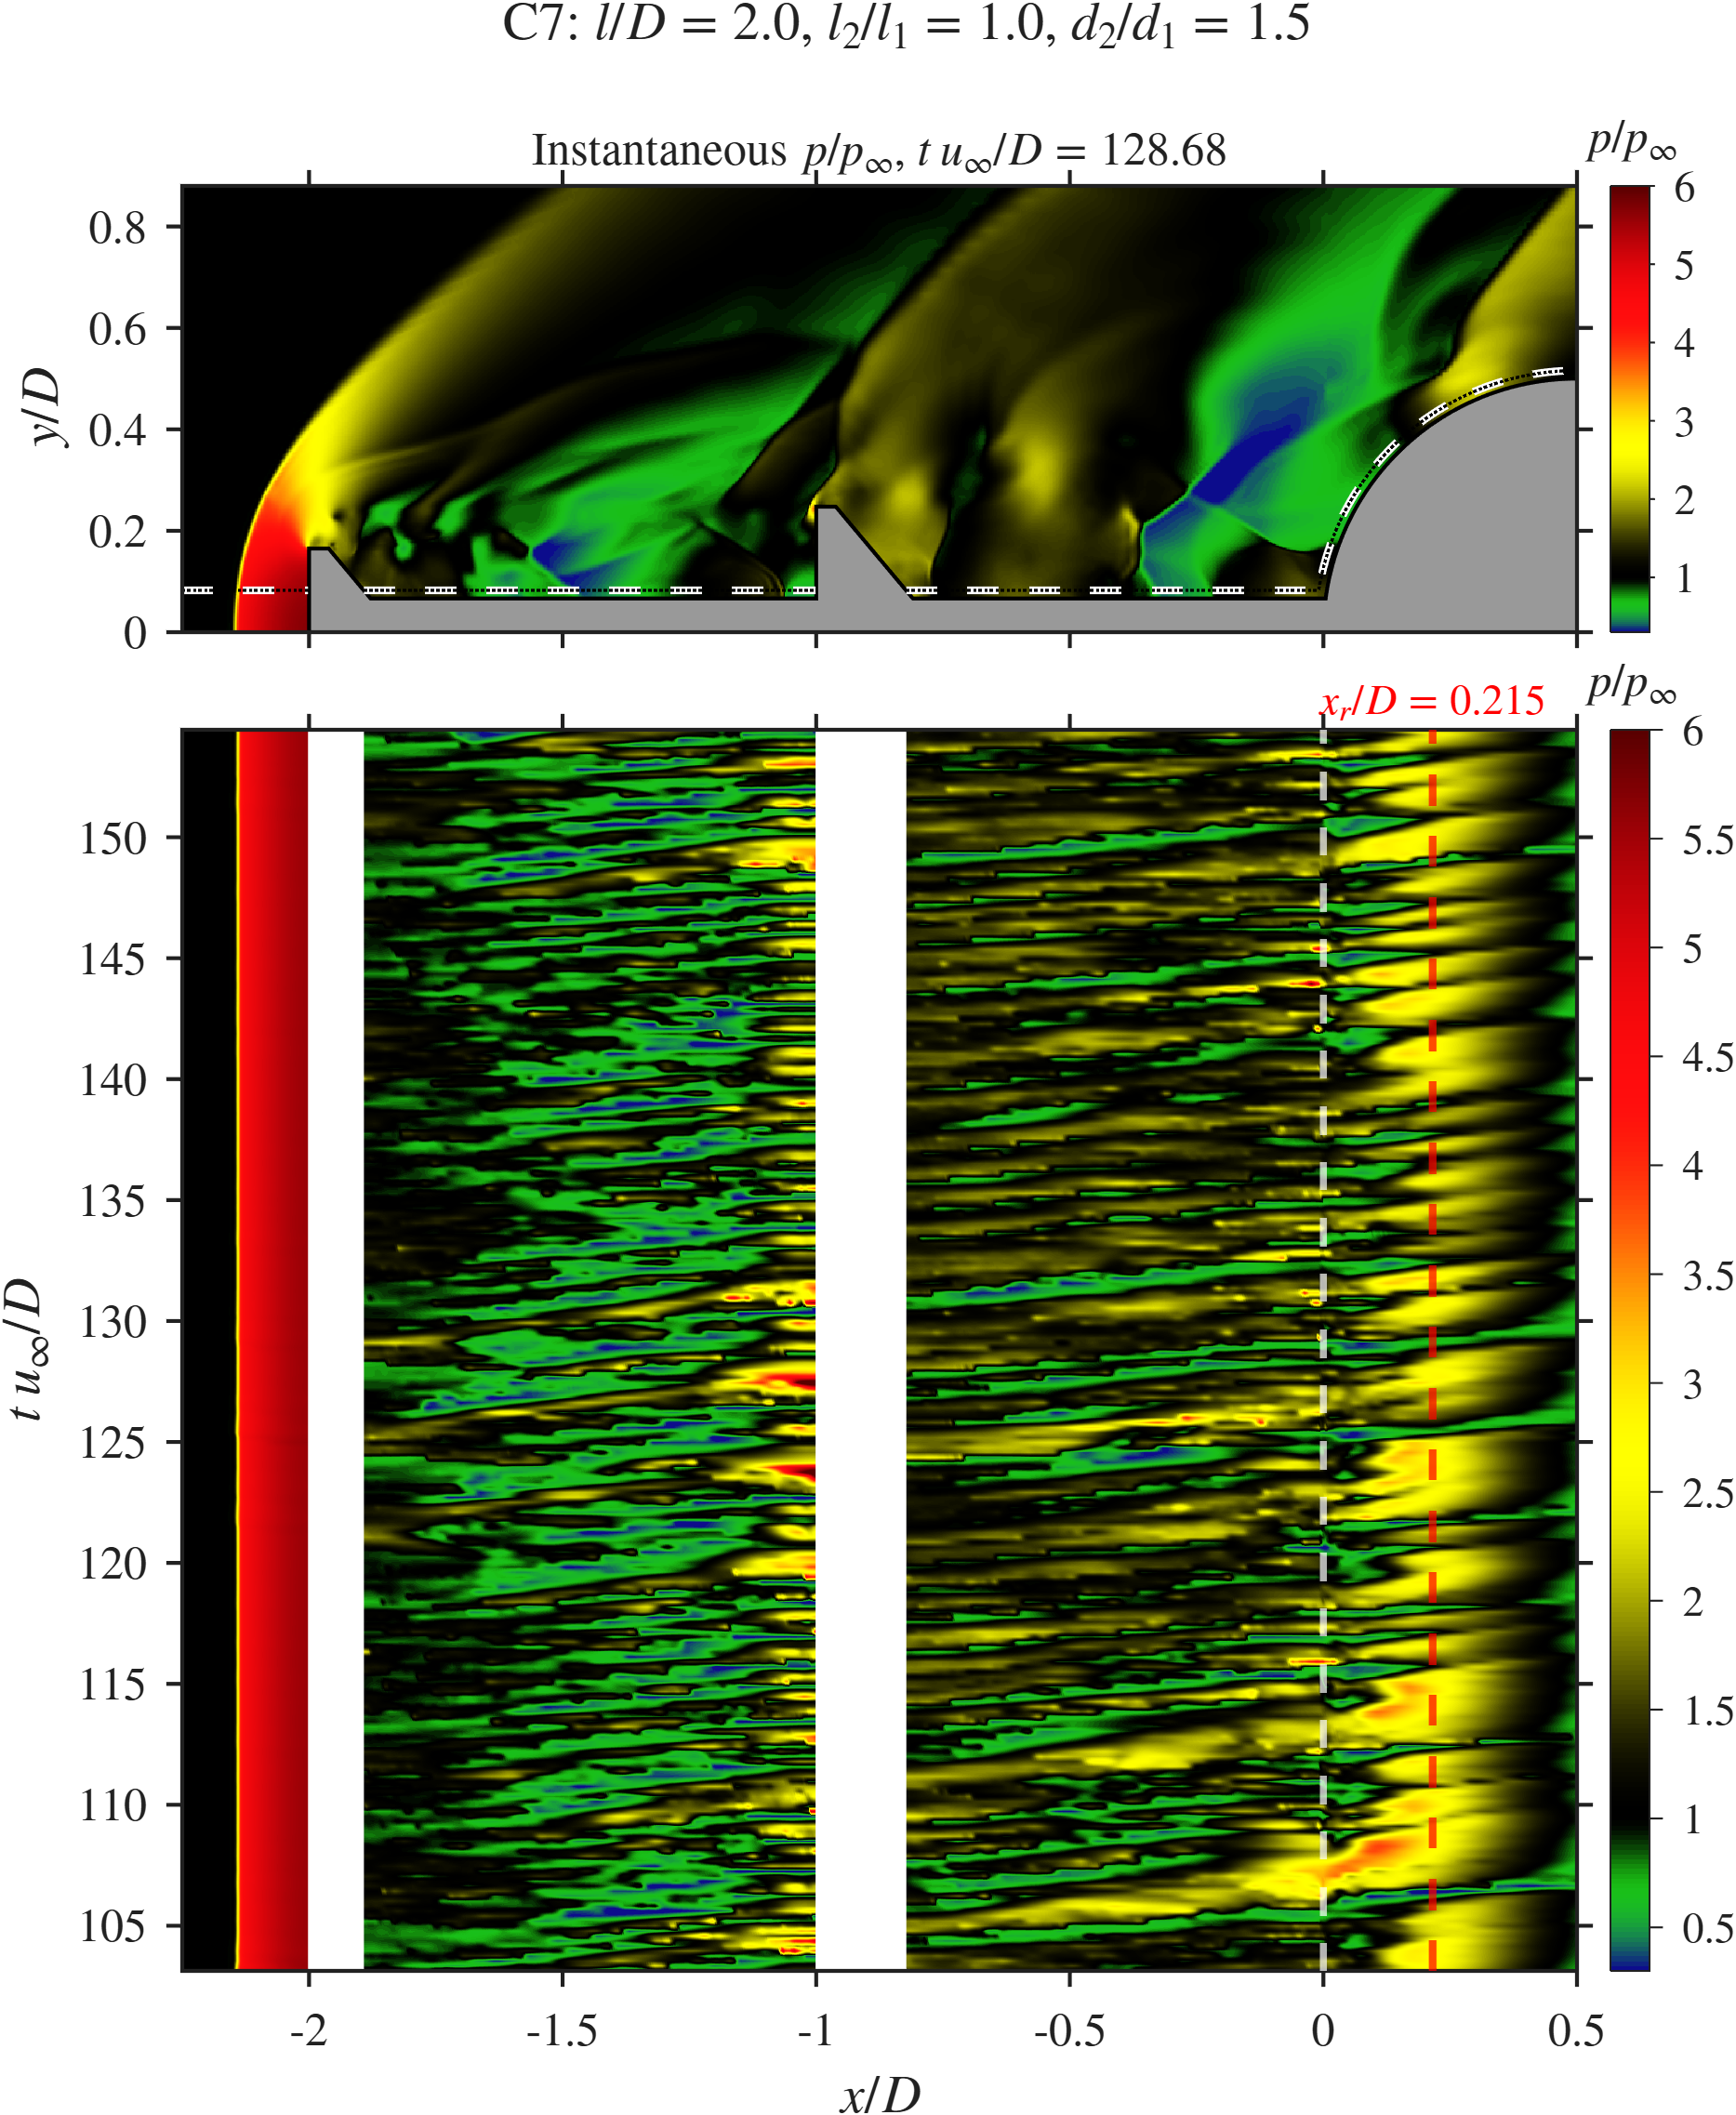
\includegraphics[width=\linewidth]{C7_xt.png}\caption{C7}\end{subfigure}
  \caption{Spike-length sweep: $x$--$t$ diagrams of $p/\pinf$ along the probe line.}
  \label{fig:len_xt}
\end{figure}

\begin{figure}[htbp]
  \centering
  \begin{subfigure}{0.325\textwidth}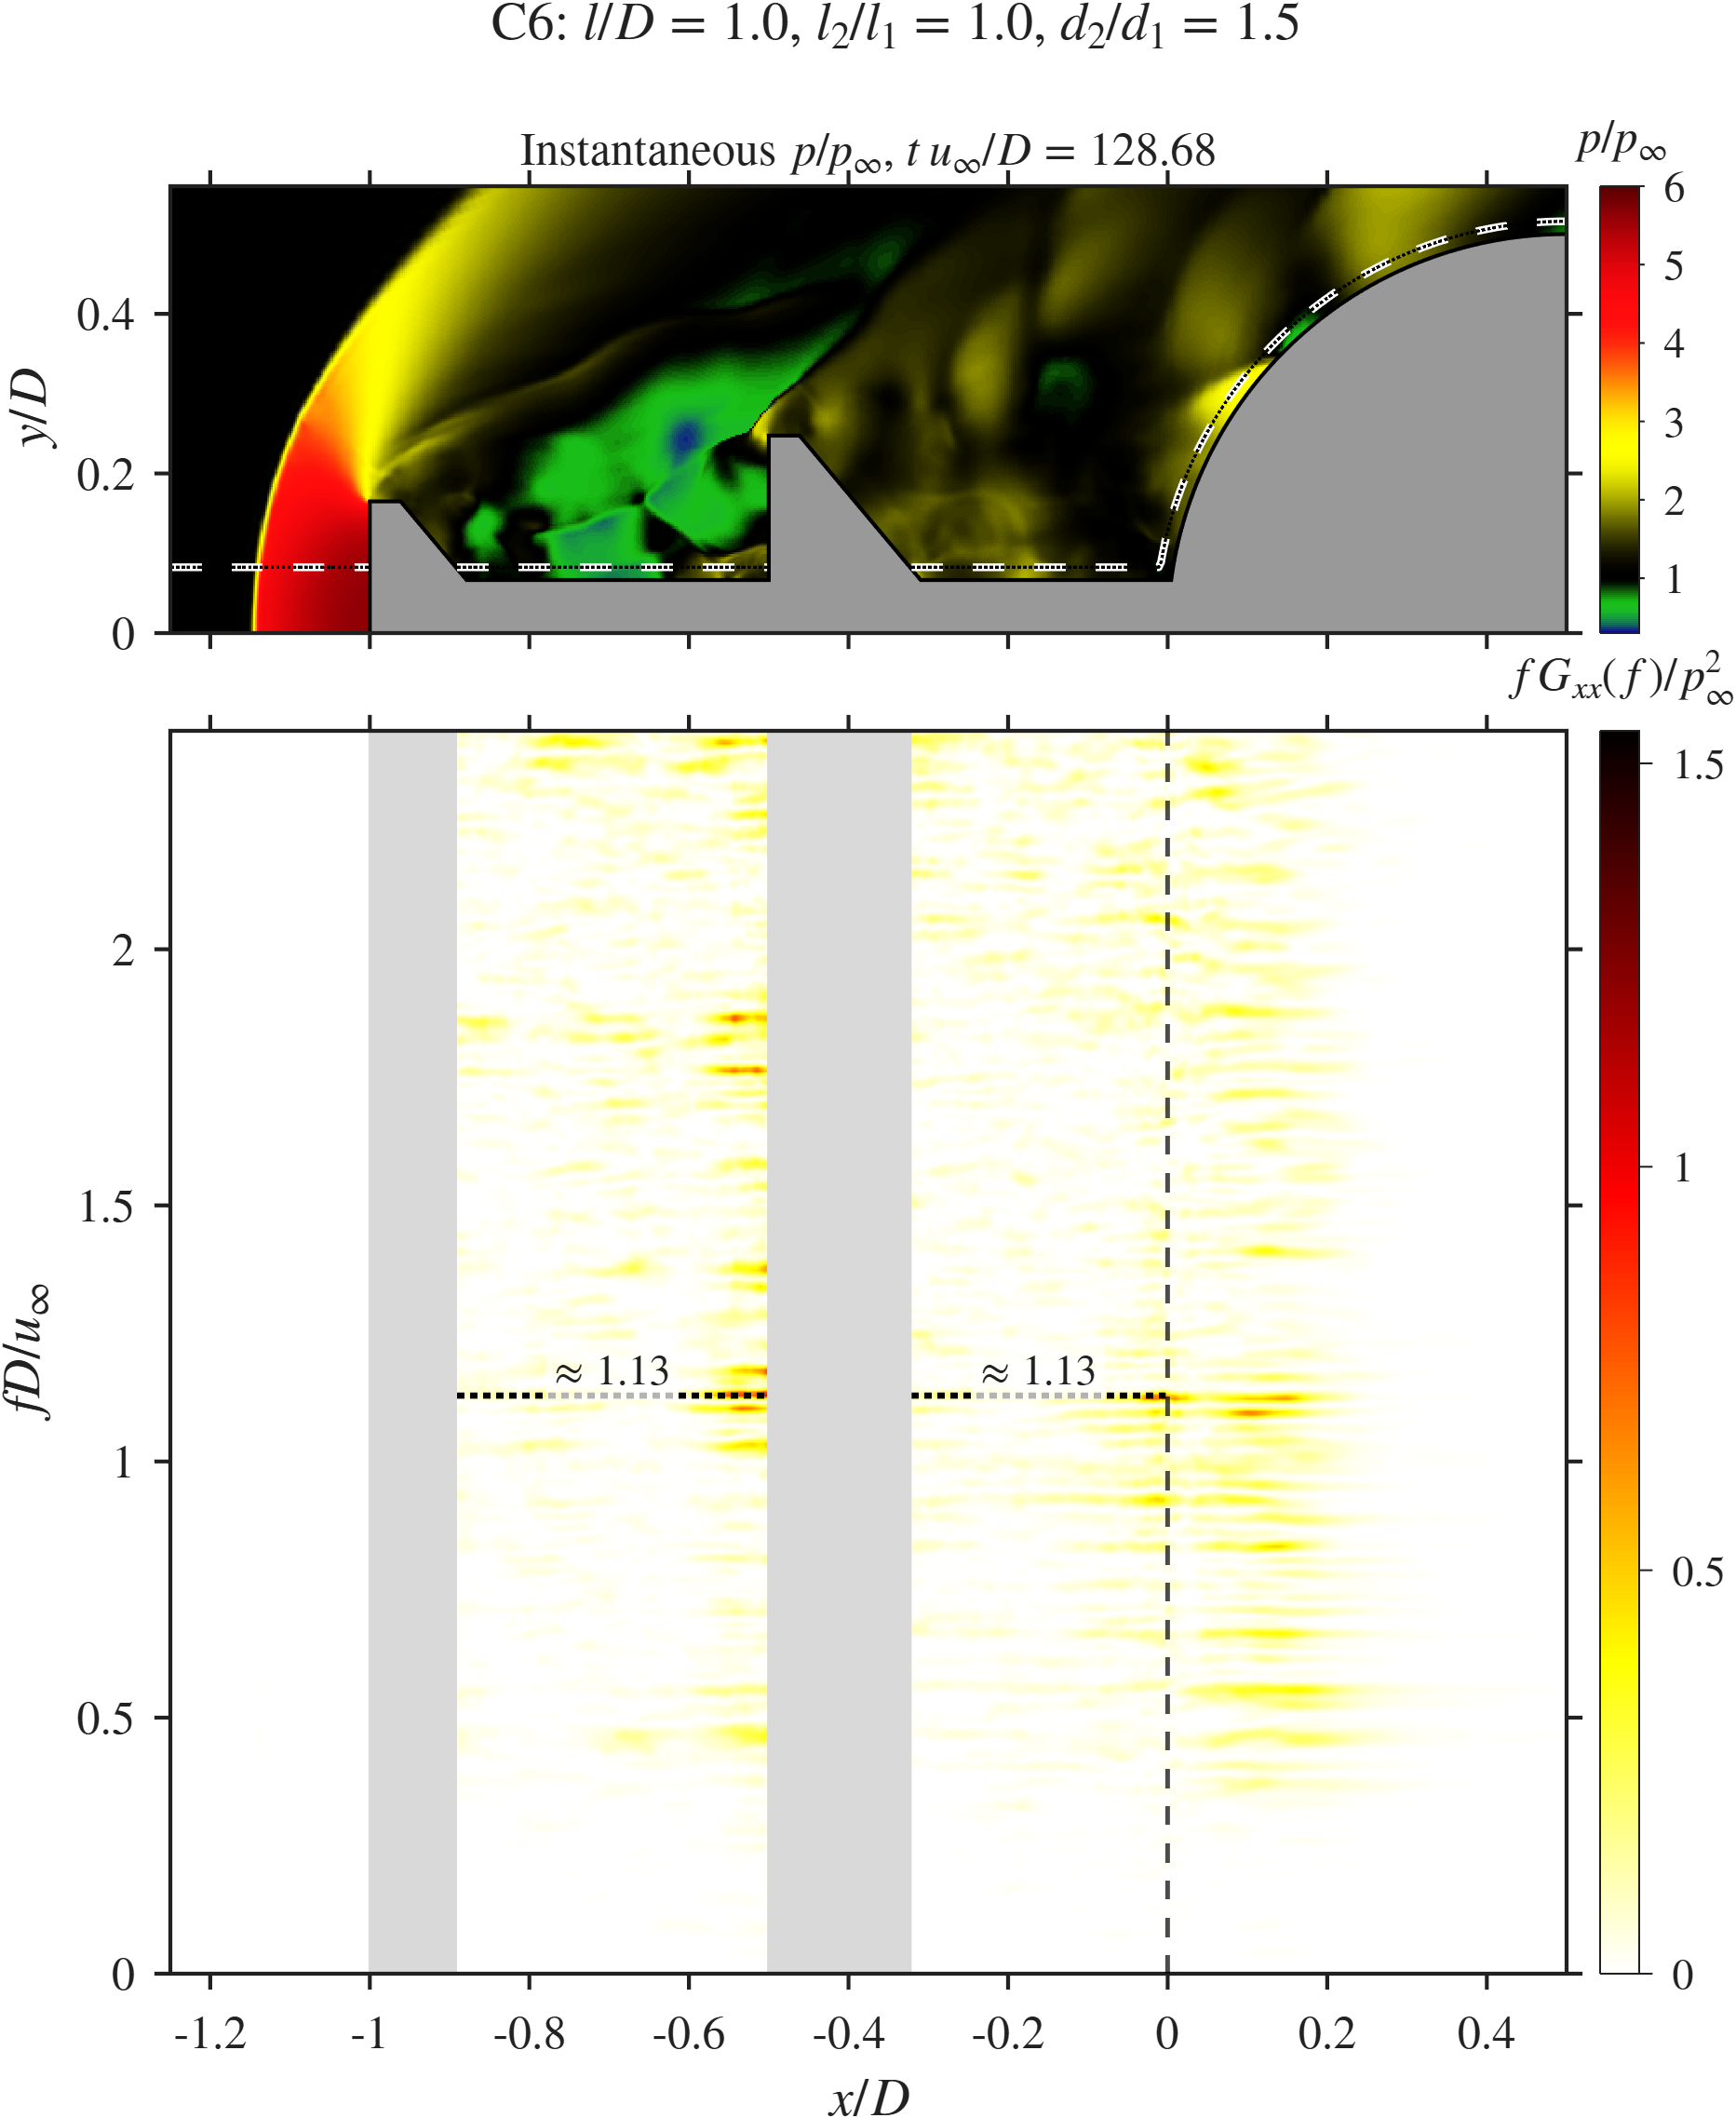
\includegraphics[width=\linewidth]{C6_xf.png}\caption{C6}\end{subfigure}
  \begin{subfigure}{0.325\textwidth}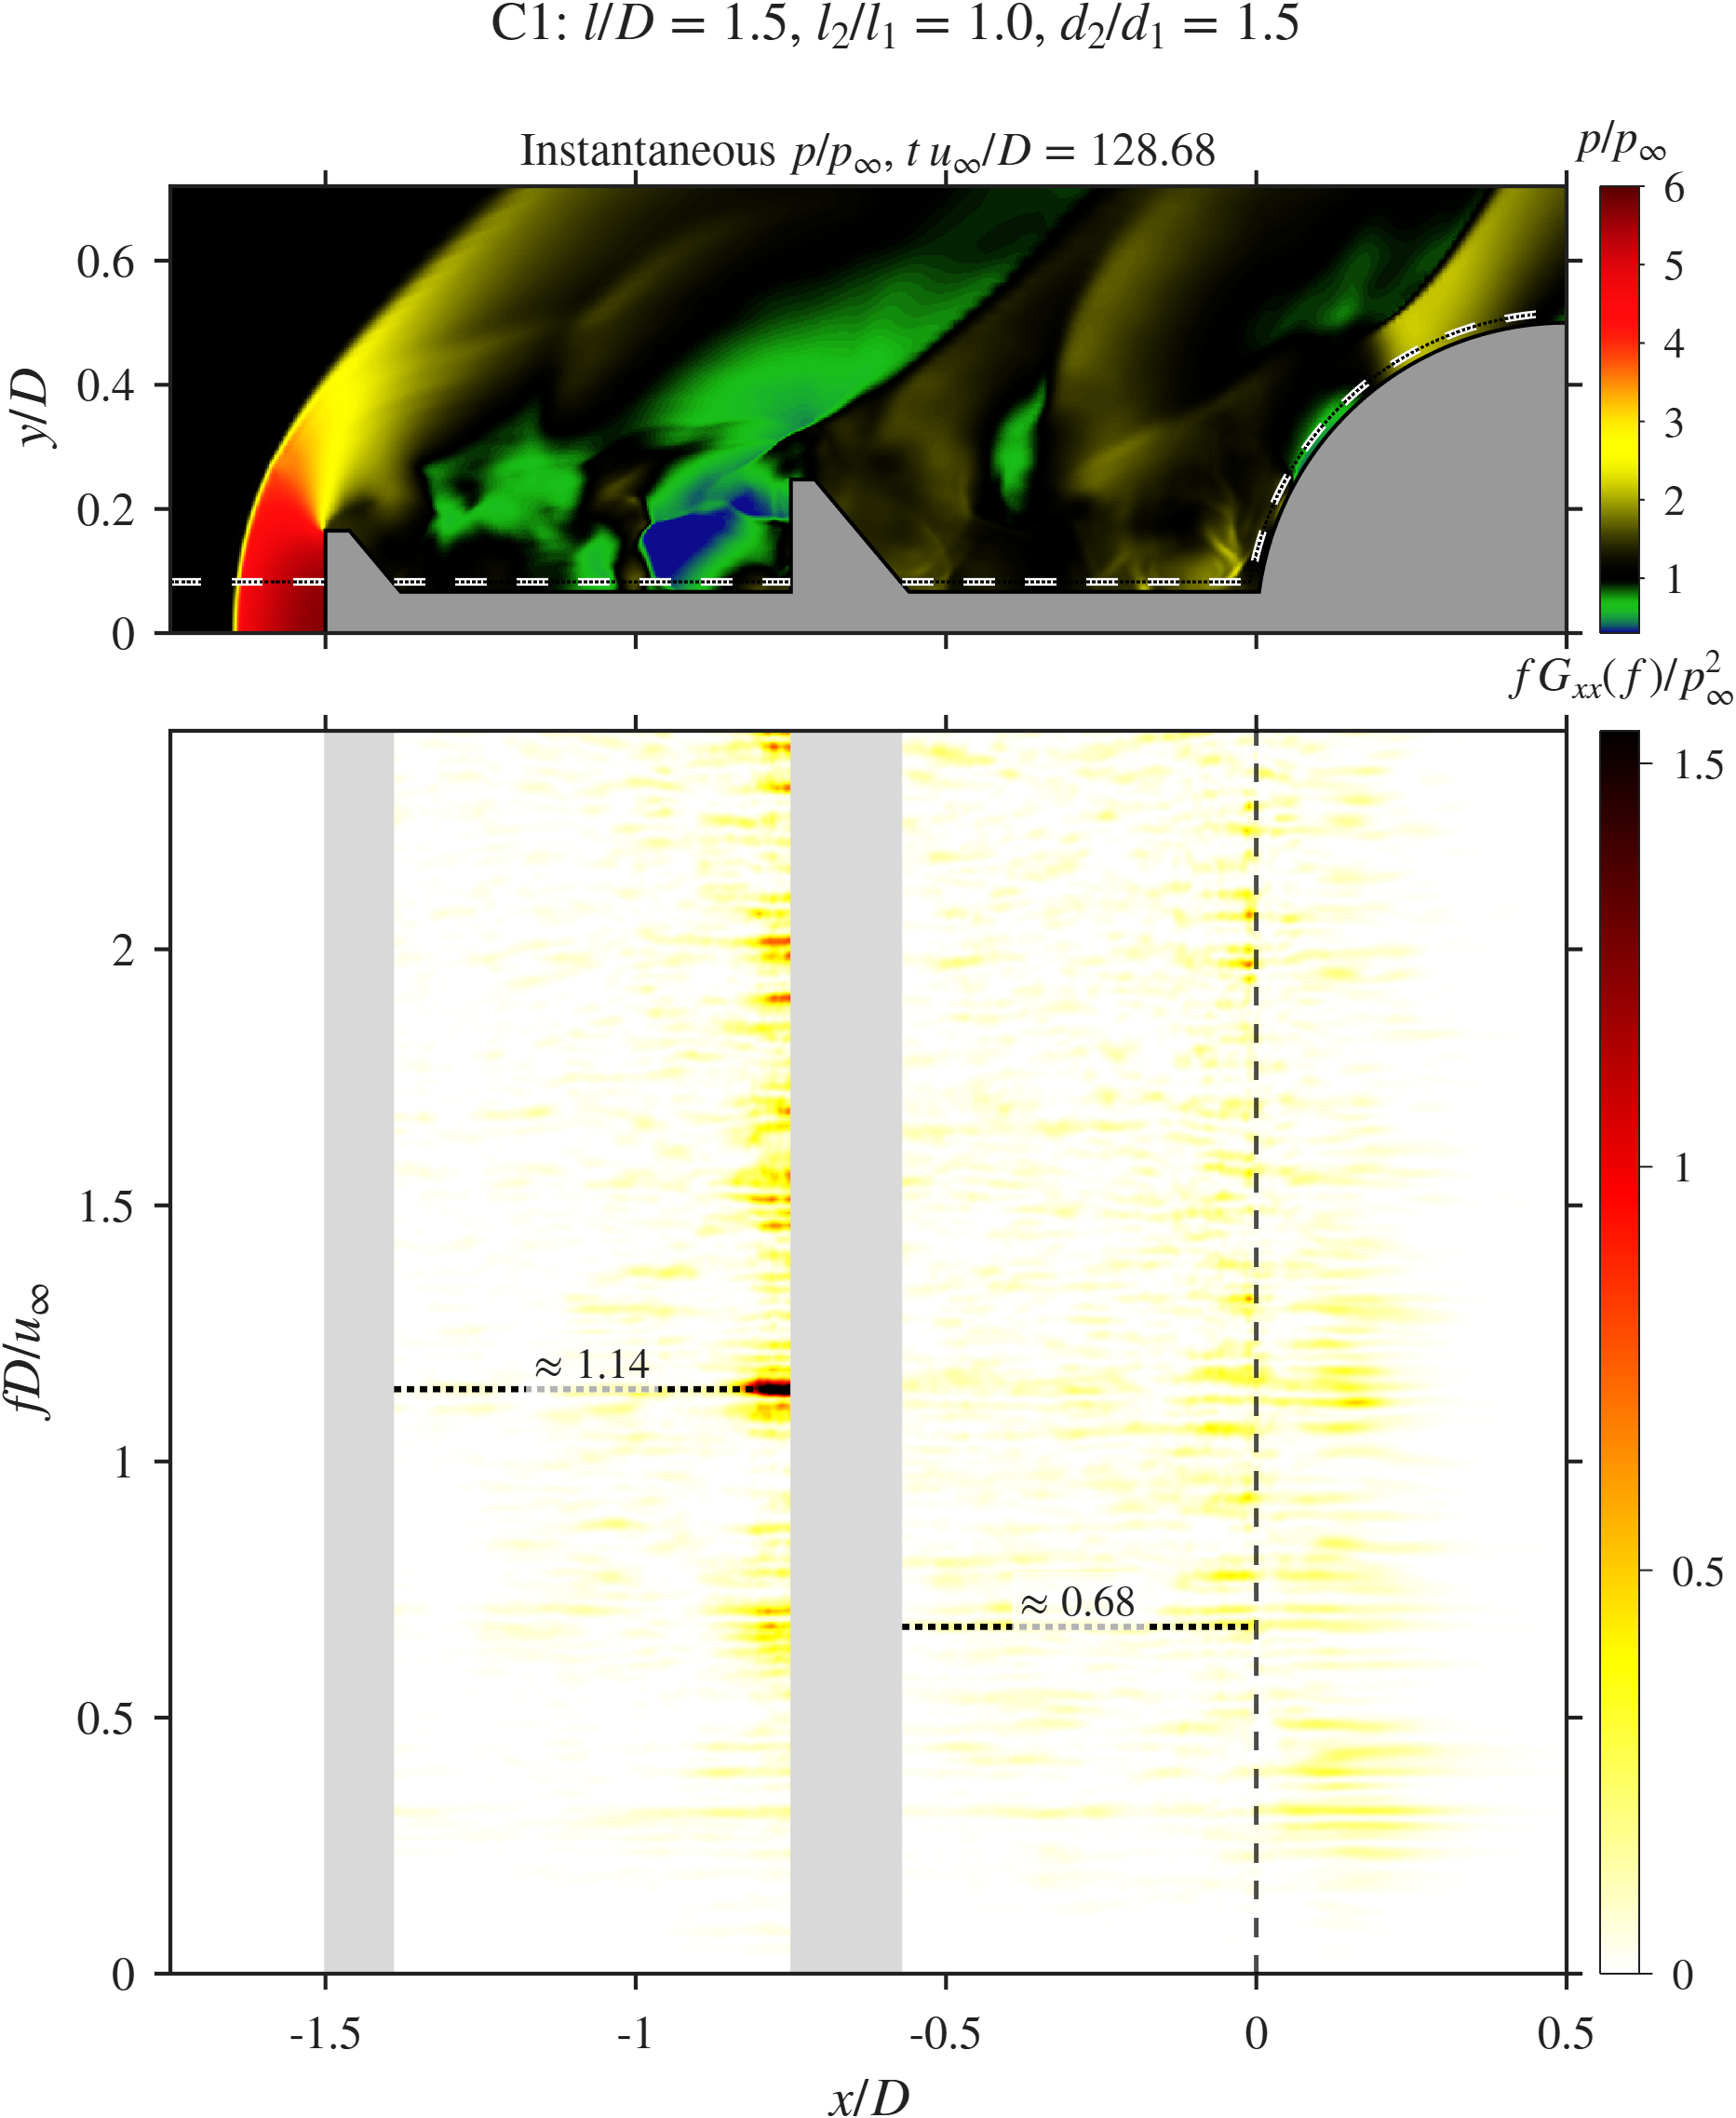
\includegraphics[width=\linewidth]{C1_xf.png}\caption{C1}\end{subfigure}
  \begin{subfigure}{0.325\textwidth}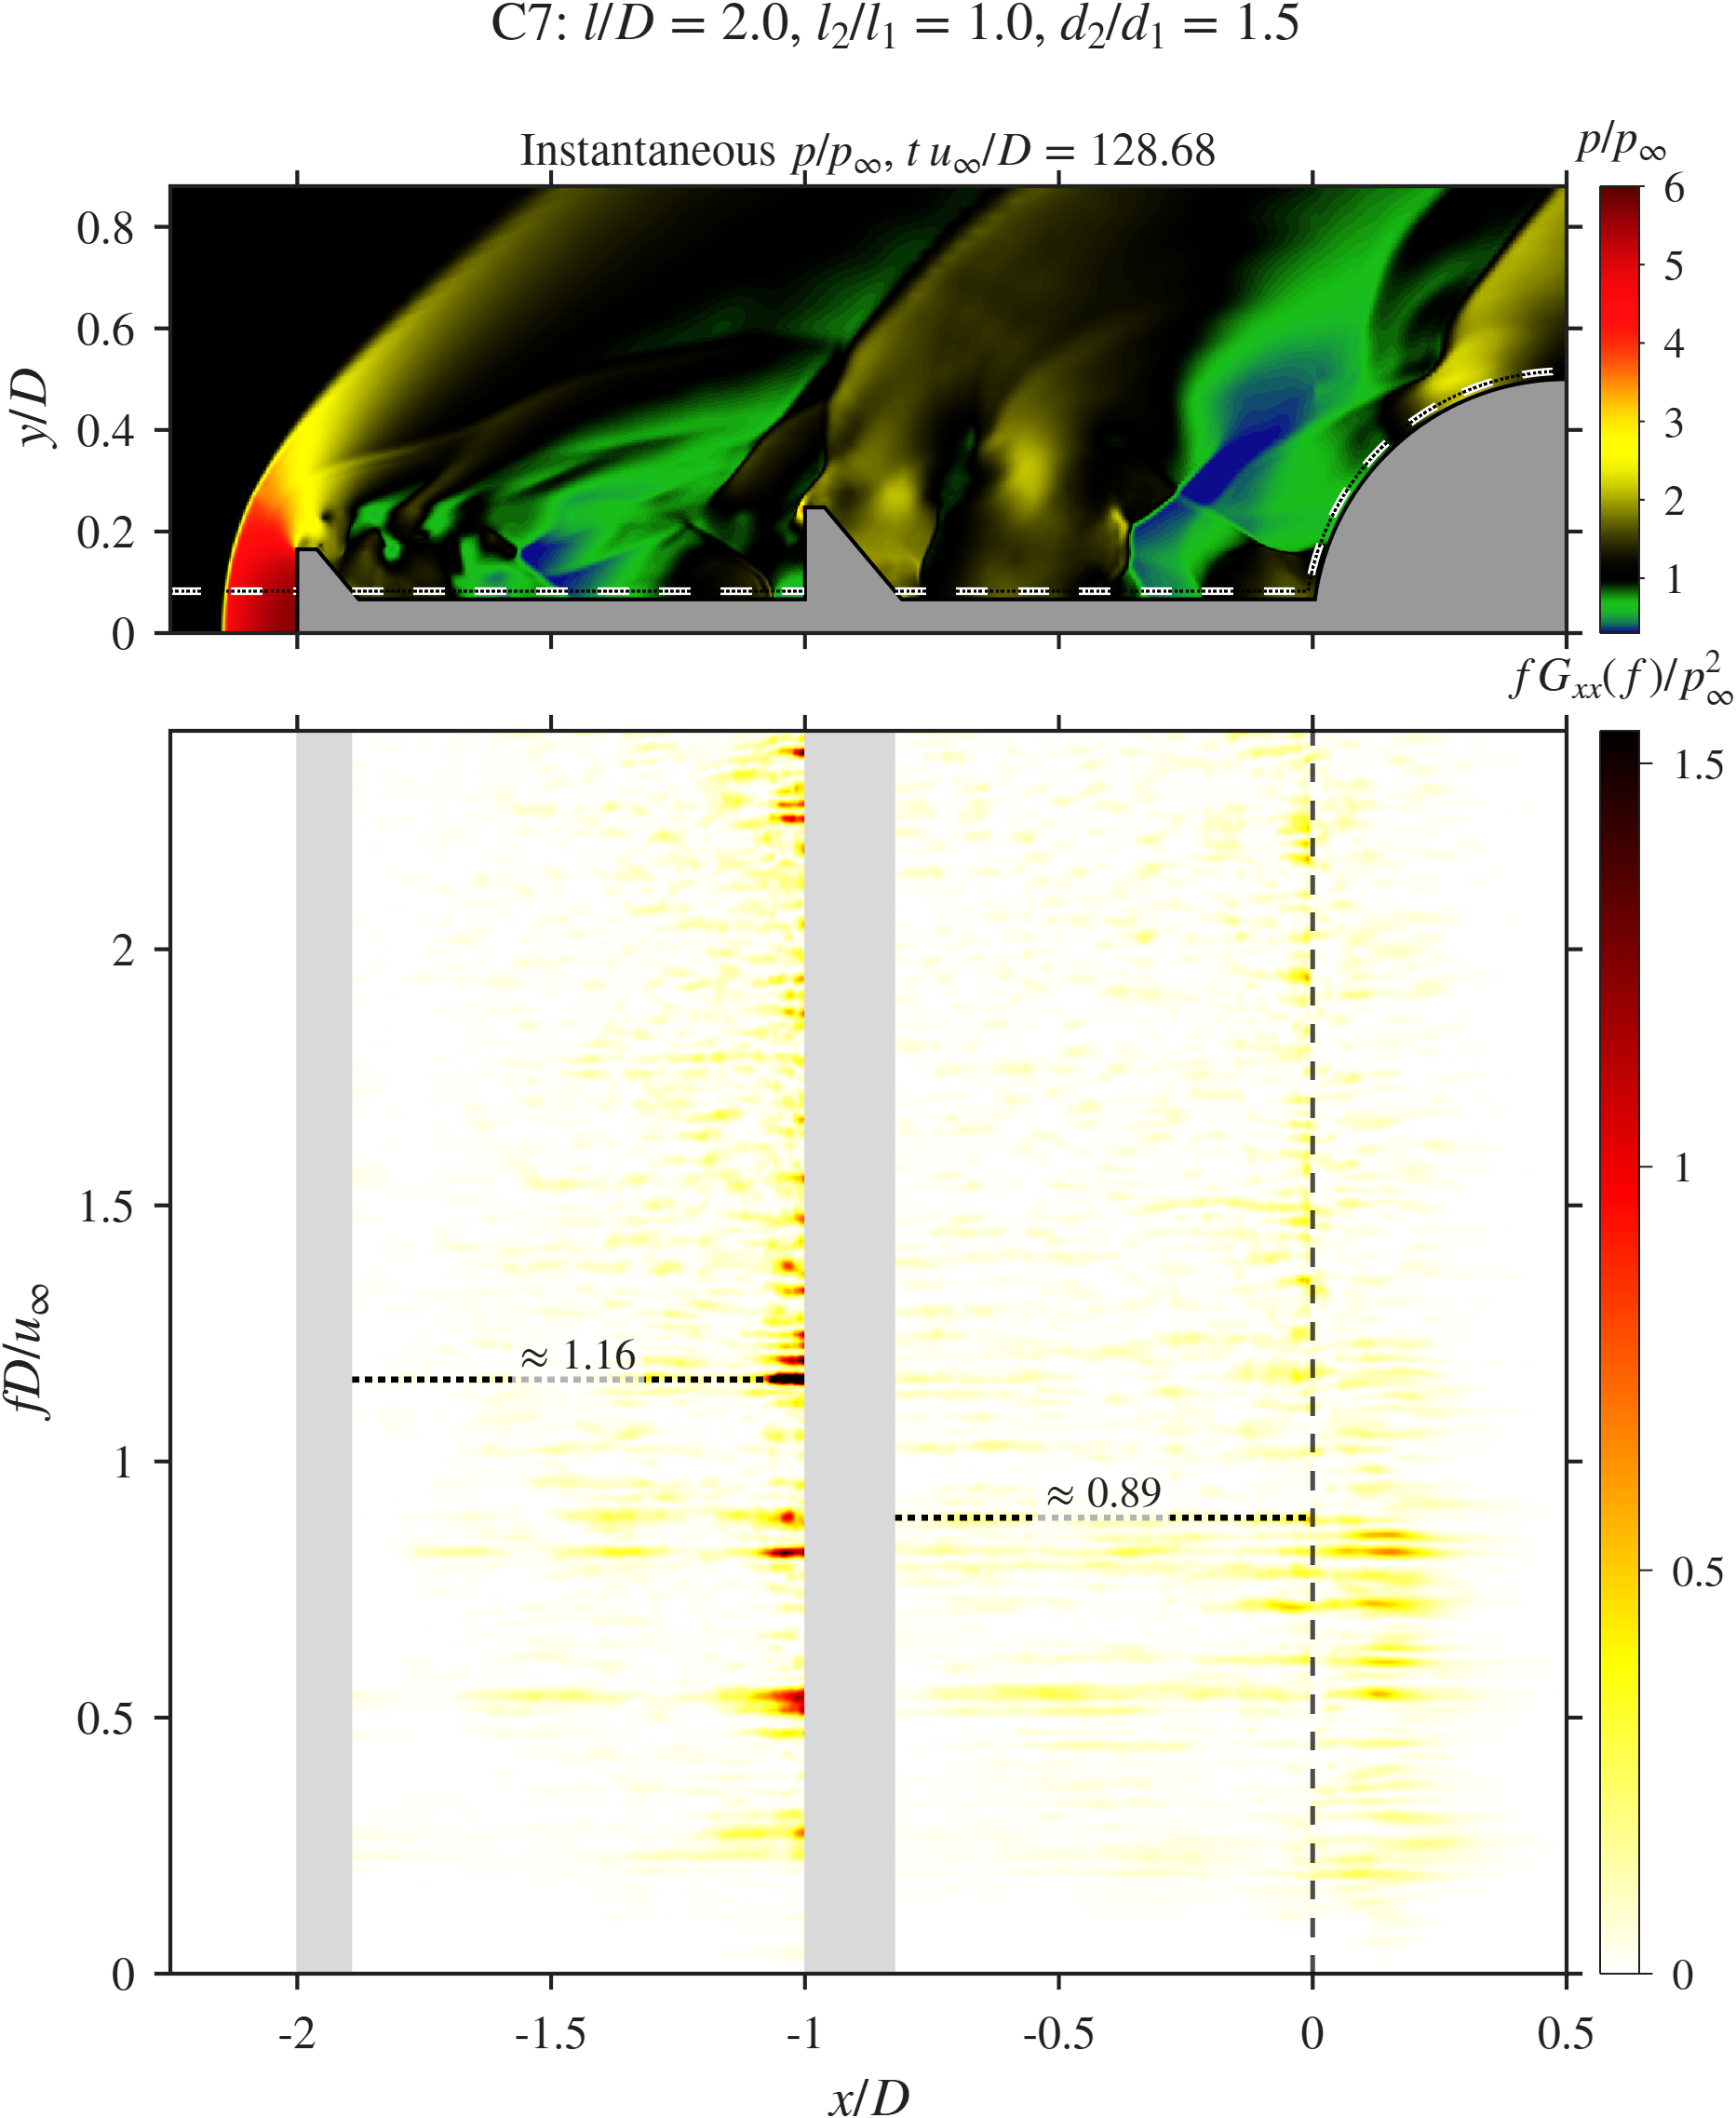
\includegraphics[width=\linewidth]{C7_xf.png}\caption{C7}\end{subfigure}
  \caption{Spike-length sweep: $x$--$f$ diagrams along the probe line.}
  \label{fig:len_xf}
\end{figure}

\paragraph{Probe signals and spectra.} Figure~\ref{fig:len_sig} shows the signals. C6 has a peak at $St = 1.13$ with $\Pi \approx 0.50$, and its drag peaks at the same frequency ($St = 1.12$). The short geometry gives a short feedback path and a fast loop. The drag fluctuation of C6 ($\sCd = 0.09$) is the lowest of all cases and below SA (0.10), at the cost of a higher mean load. C7 has a peak at $St = 0.82$ with $\Pi \approx 0.54$, and its drag peaks at the same $St$. The lower frequency fits the longer path: both the convection time down the shear layer and the time for disturbances to travel upstream grow with the spike length. The drag fluctuation of C7 ($\sCd = 0.16$) is 78\% higher than C6, consistent with the larger structures that grow on the longer shear layer.

The product $St\,(l/D)$ is 1.13 (C6), 1.68 (C1) and 1.64 (C7). It is nearly constant for C1 and C7, which suggests that for $l/D \ge 1.5$ the feedback frequency scales with the total spike length. C6 departs from this, which may point to a change toward pulsation-dominated behaviour for short spikes \chk{CHECK: link to the mode change with $l/D$ in~\cite{Panaras2009highspeed} if the paper supports it}.

\begin{figure}[htbp]
  \centering
  \begin{subfigure}{\textwidth}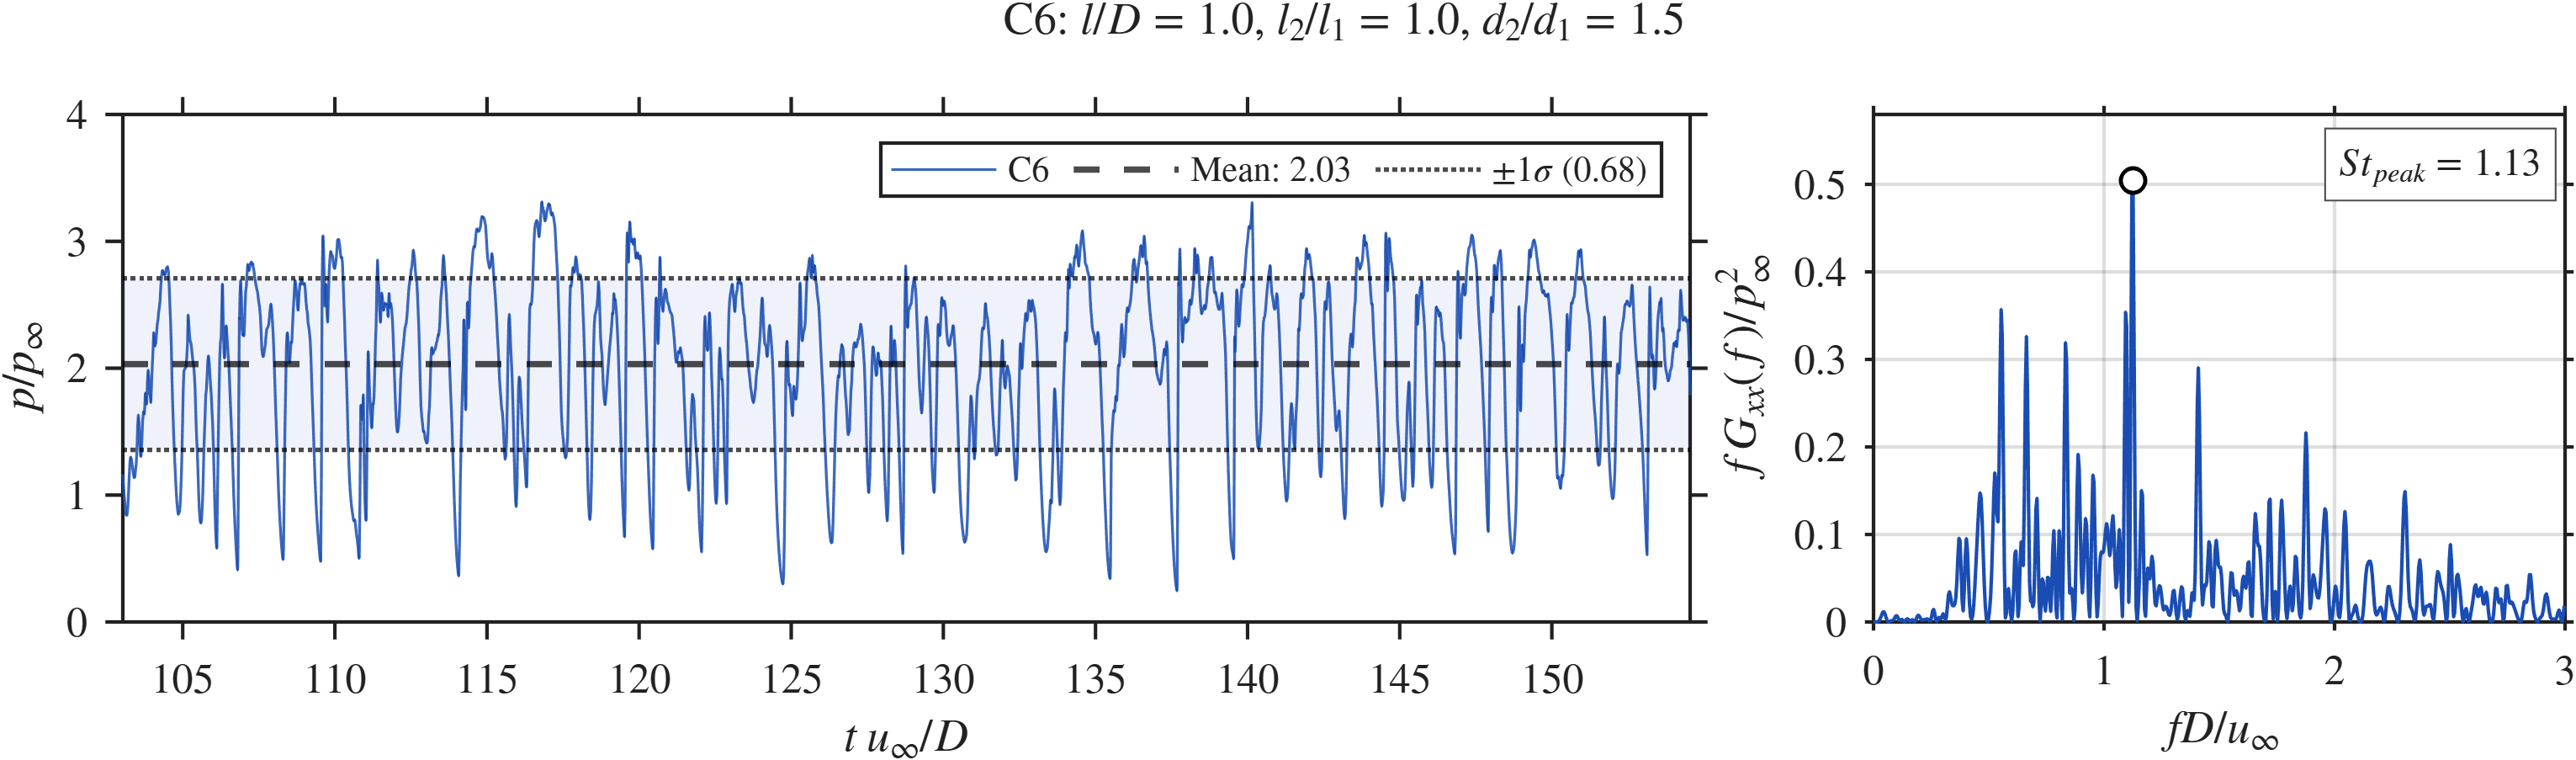
\includegraphics[width=\linewidth]{C6_psig.png}\caption{C6, pressure}\end{subfigure}\\
  \begin{subfigure}{\textwidth}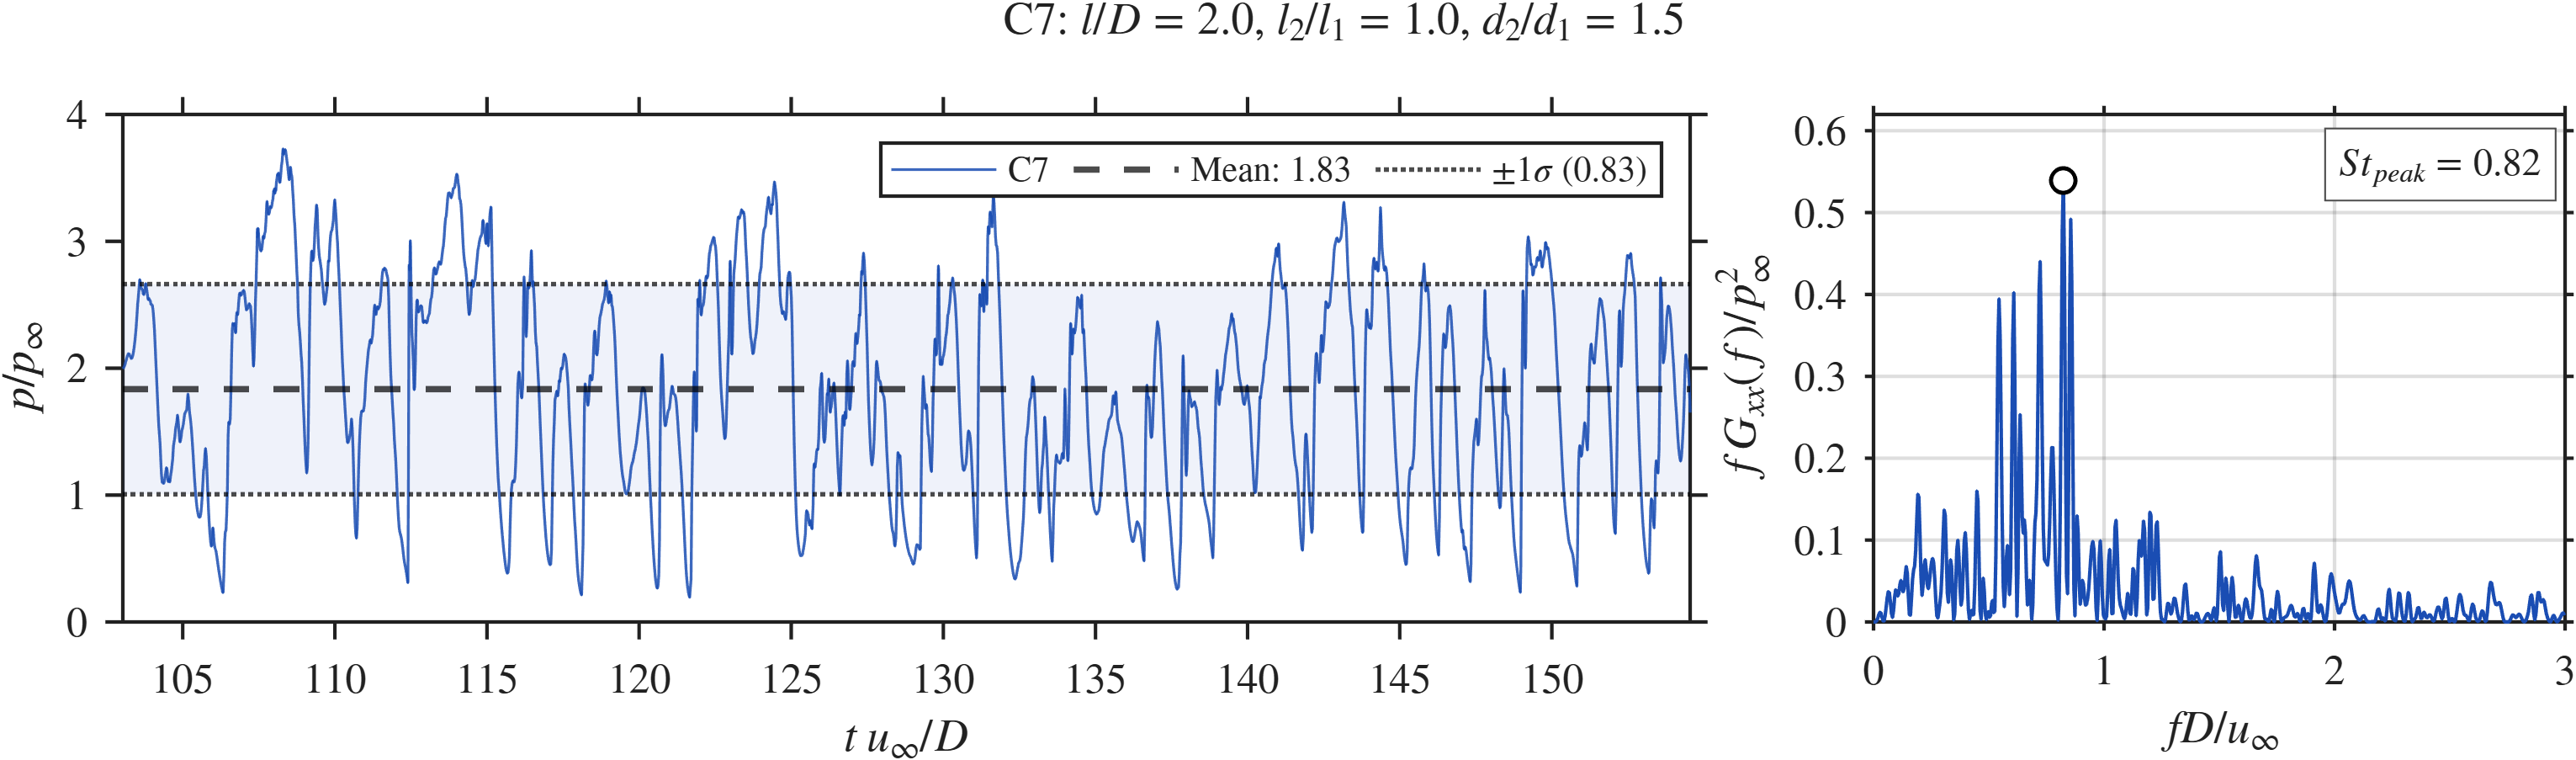
\includegraphics[width=\linewidth]{C7_psig.png}\caption{C7, pressure}\end{subfigure}\\
  \begin{subfigure}{\textwidth}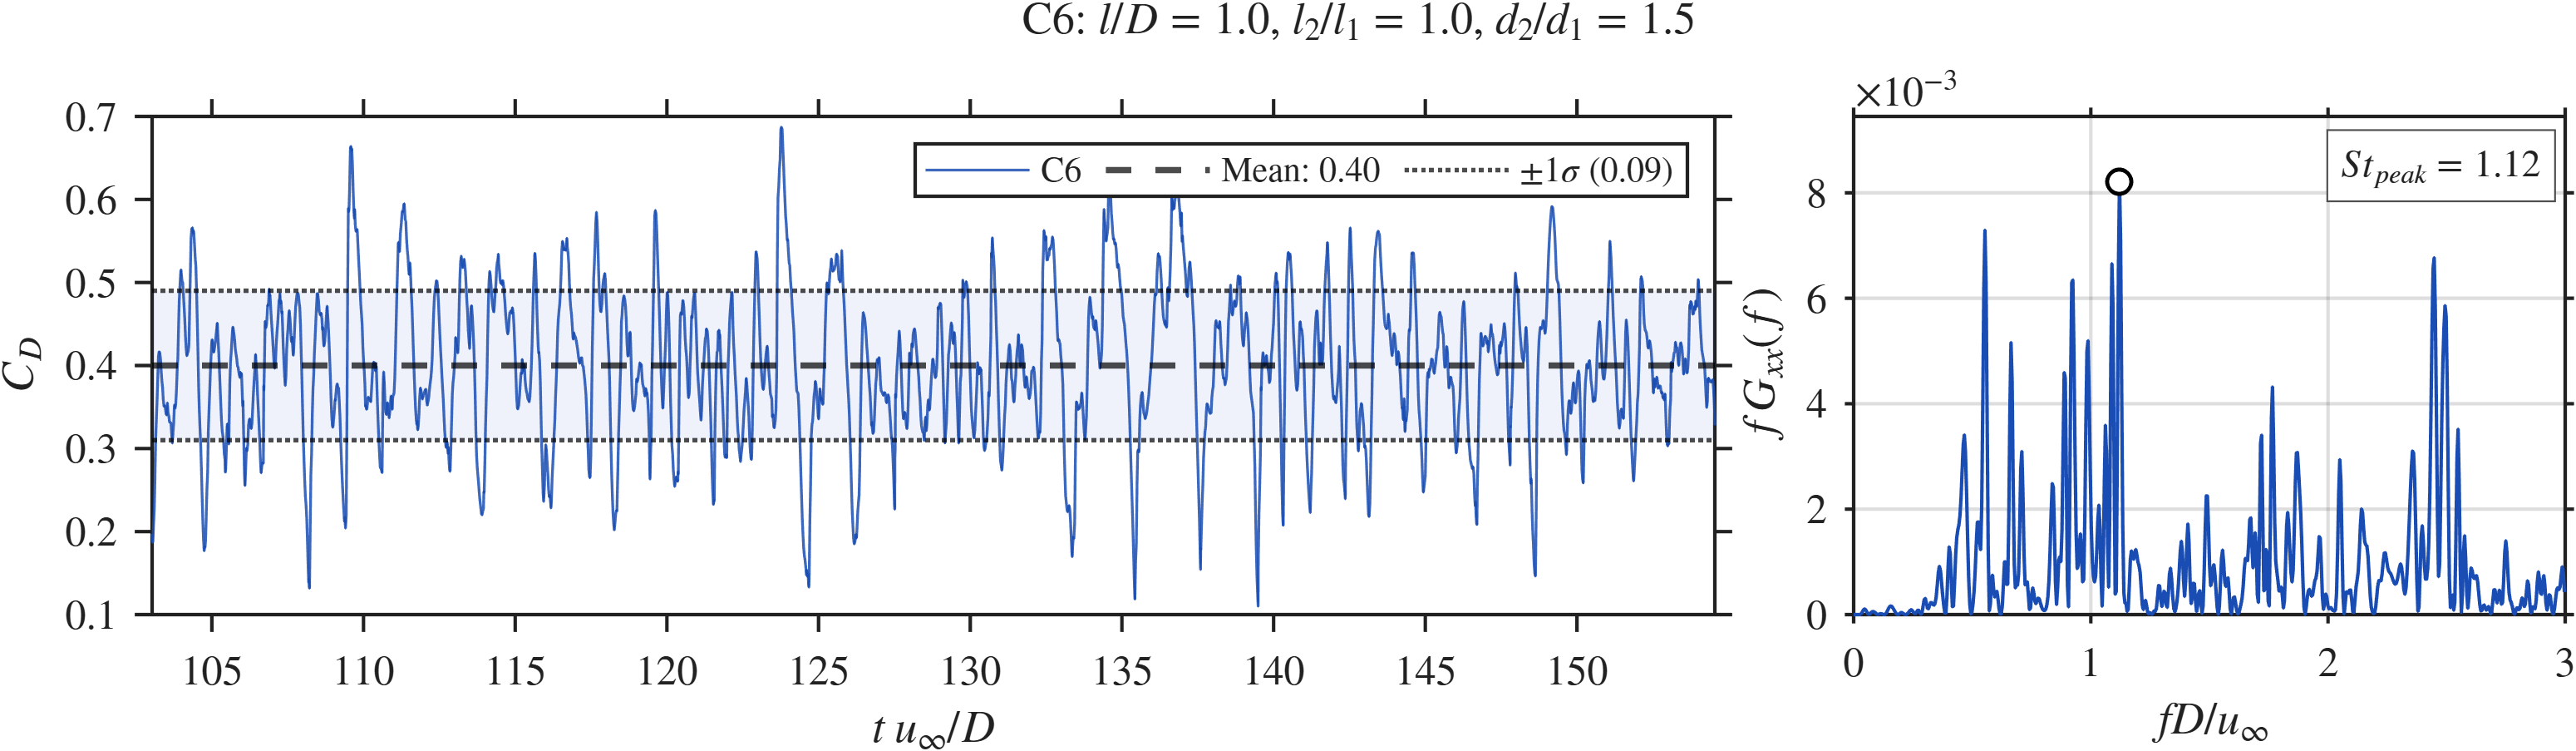
\includegraphics[width=\linewidth]{C6_dsig.png}\caption{C6, drag}\end{subfigure}\\
  \begin{subfigure}{\textwidth}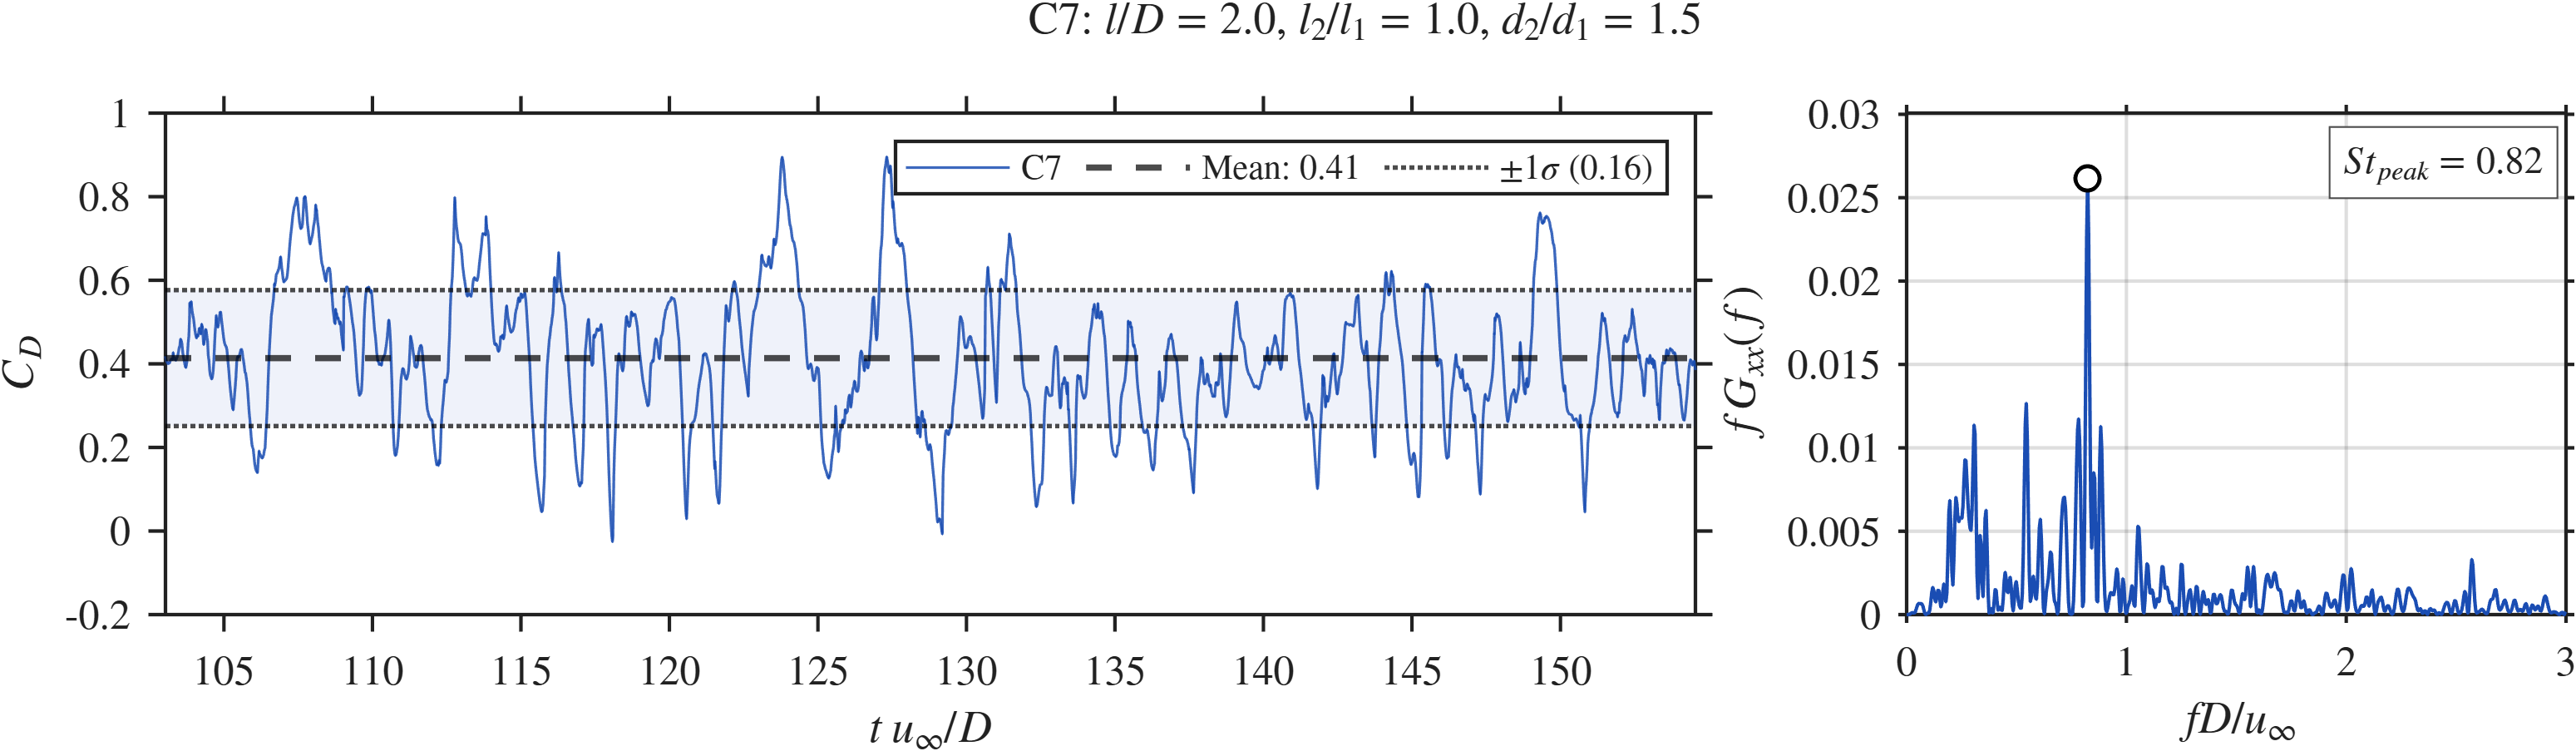
\includegraphics[width=\linewidth]{C7_dsig.png}\caption{C7, drag}\end{subfigure}
  \caption{Spike-length sweep: probe pressure and drag signals with spectra for C6 and C7.}
  \label{fig:len_sig}
\end{figure}

\paragraph{SPOD.} Figure~\ref{fig:len_spod} shows the SPOD results. C6 has the lowest peak of all cases ($\lambda_1 \approx 6\times10^{-6}$ at $St = 0.505$). Its leading mode is compact, confined to the short cavities, with no structures ahead of the primary disk. Its second peak at $St = 1.126$ matches the probe peak and sits at the second disk and the shoulder. The low energy and compact modes show that the short DDAS holds back the growth of large coherent structures. C7 has a peak of $\lambda_1 \approx 2.5\times10^{-5}$ at $St = 0.214$, the lowest leading frequency of any DDAS case. Its leading mode has large structures along the whole $2D$ spike, in both cavities, along the shear layer and at the shoulder, with a wide gap to the second eigenvalue. One global low-frequency oscillation therefore dominates the flow. Its other peaks at $St = 0.544$ and 0.835 show finer structures toward the shoulder. Short spikes give compact, low-energy modes and low drag fluctuation. Long spikes give large, energetic global modes and stronger pressure and drag fluctuations.

\begin{figure}[htbp]
  \centering
  \begin{subfigure}{0.72\textwidth}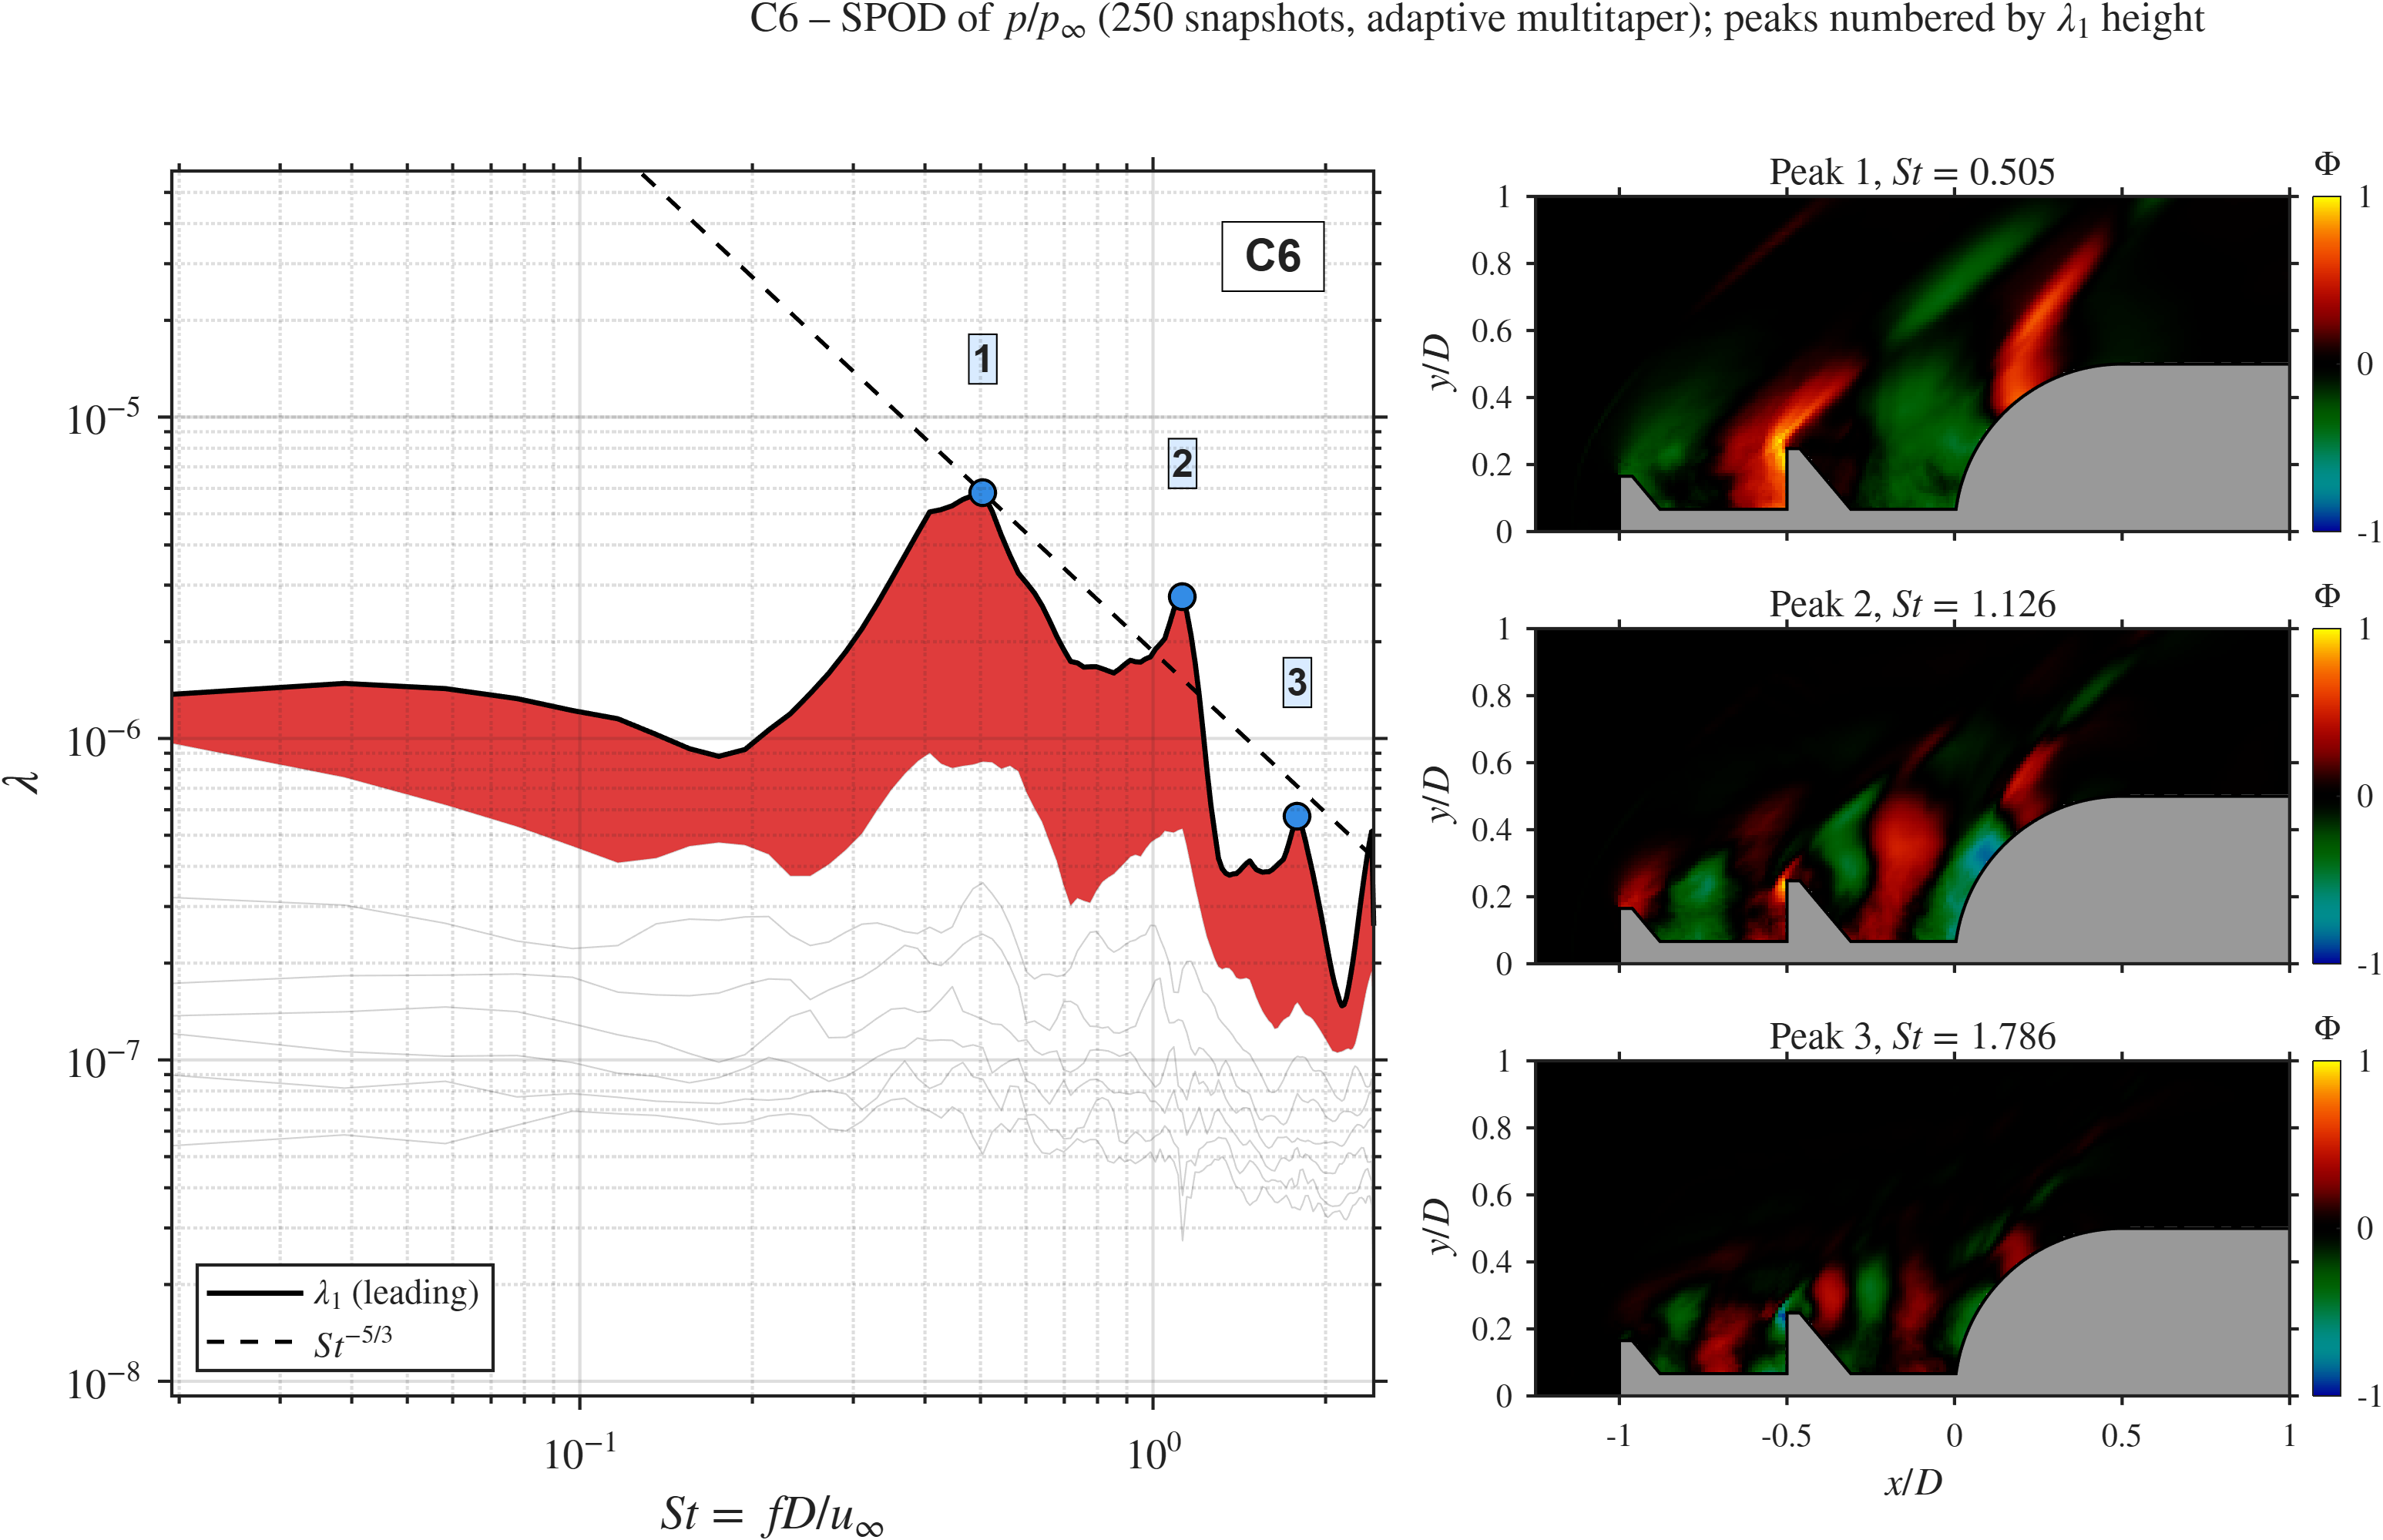
\includegraphics[width=\linewidth]{C6_spod.png}\caption{C6 ($l/D = 1$)}\end{subfigure}\\
  \begin{subfigure}{0.72\textwidth}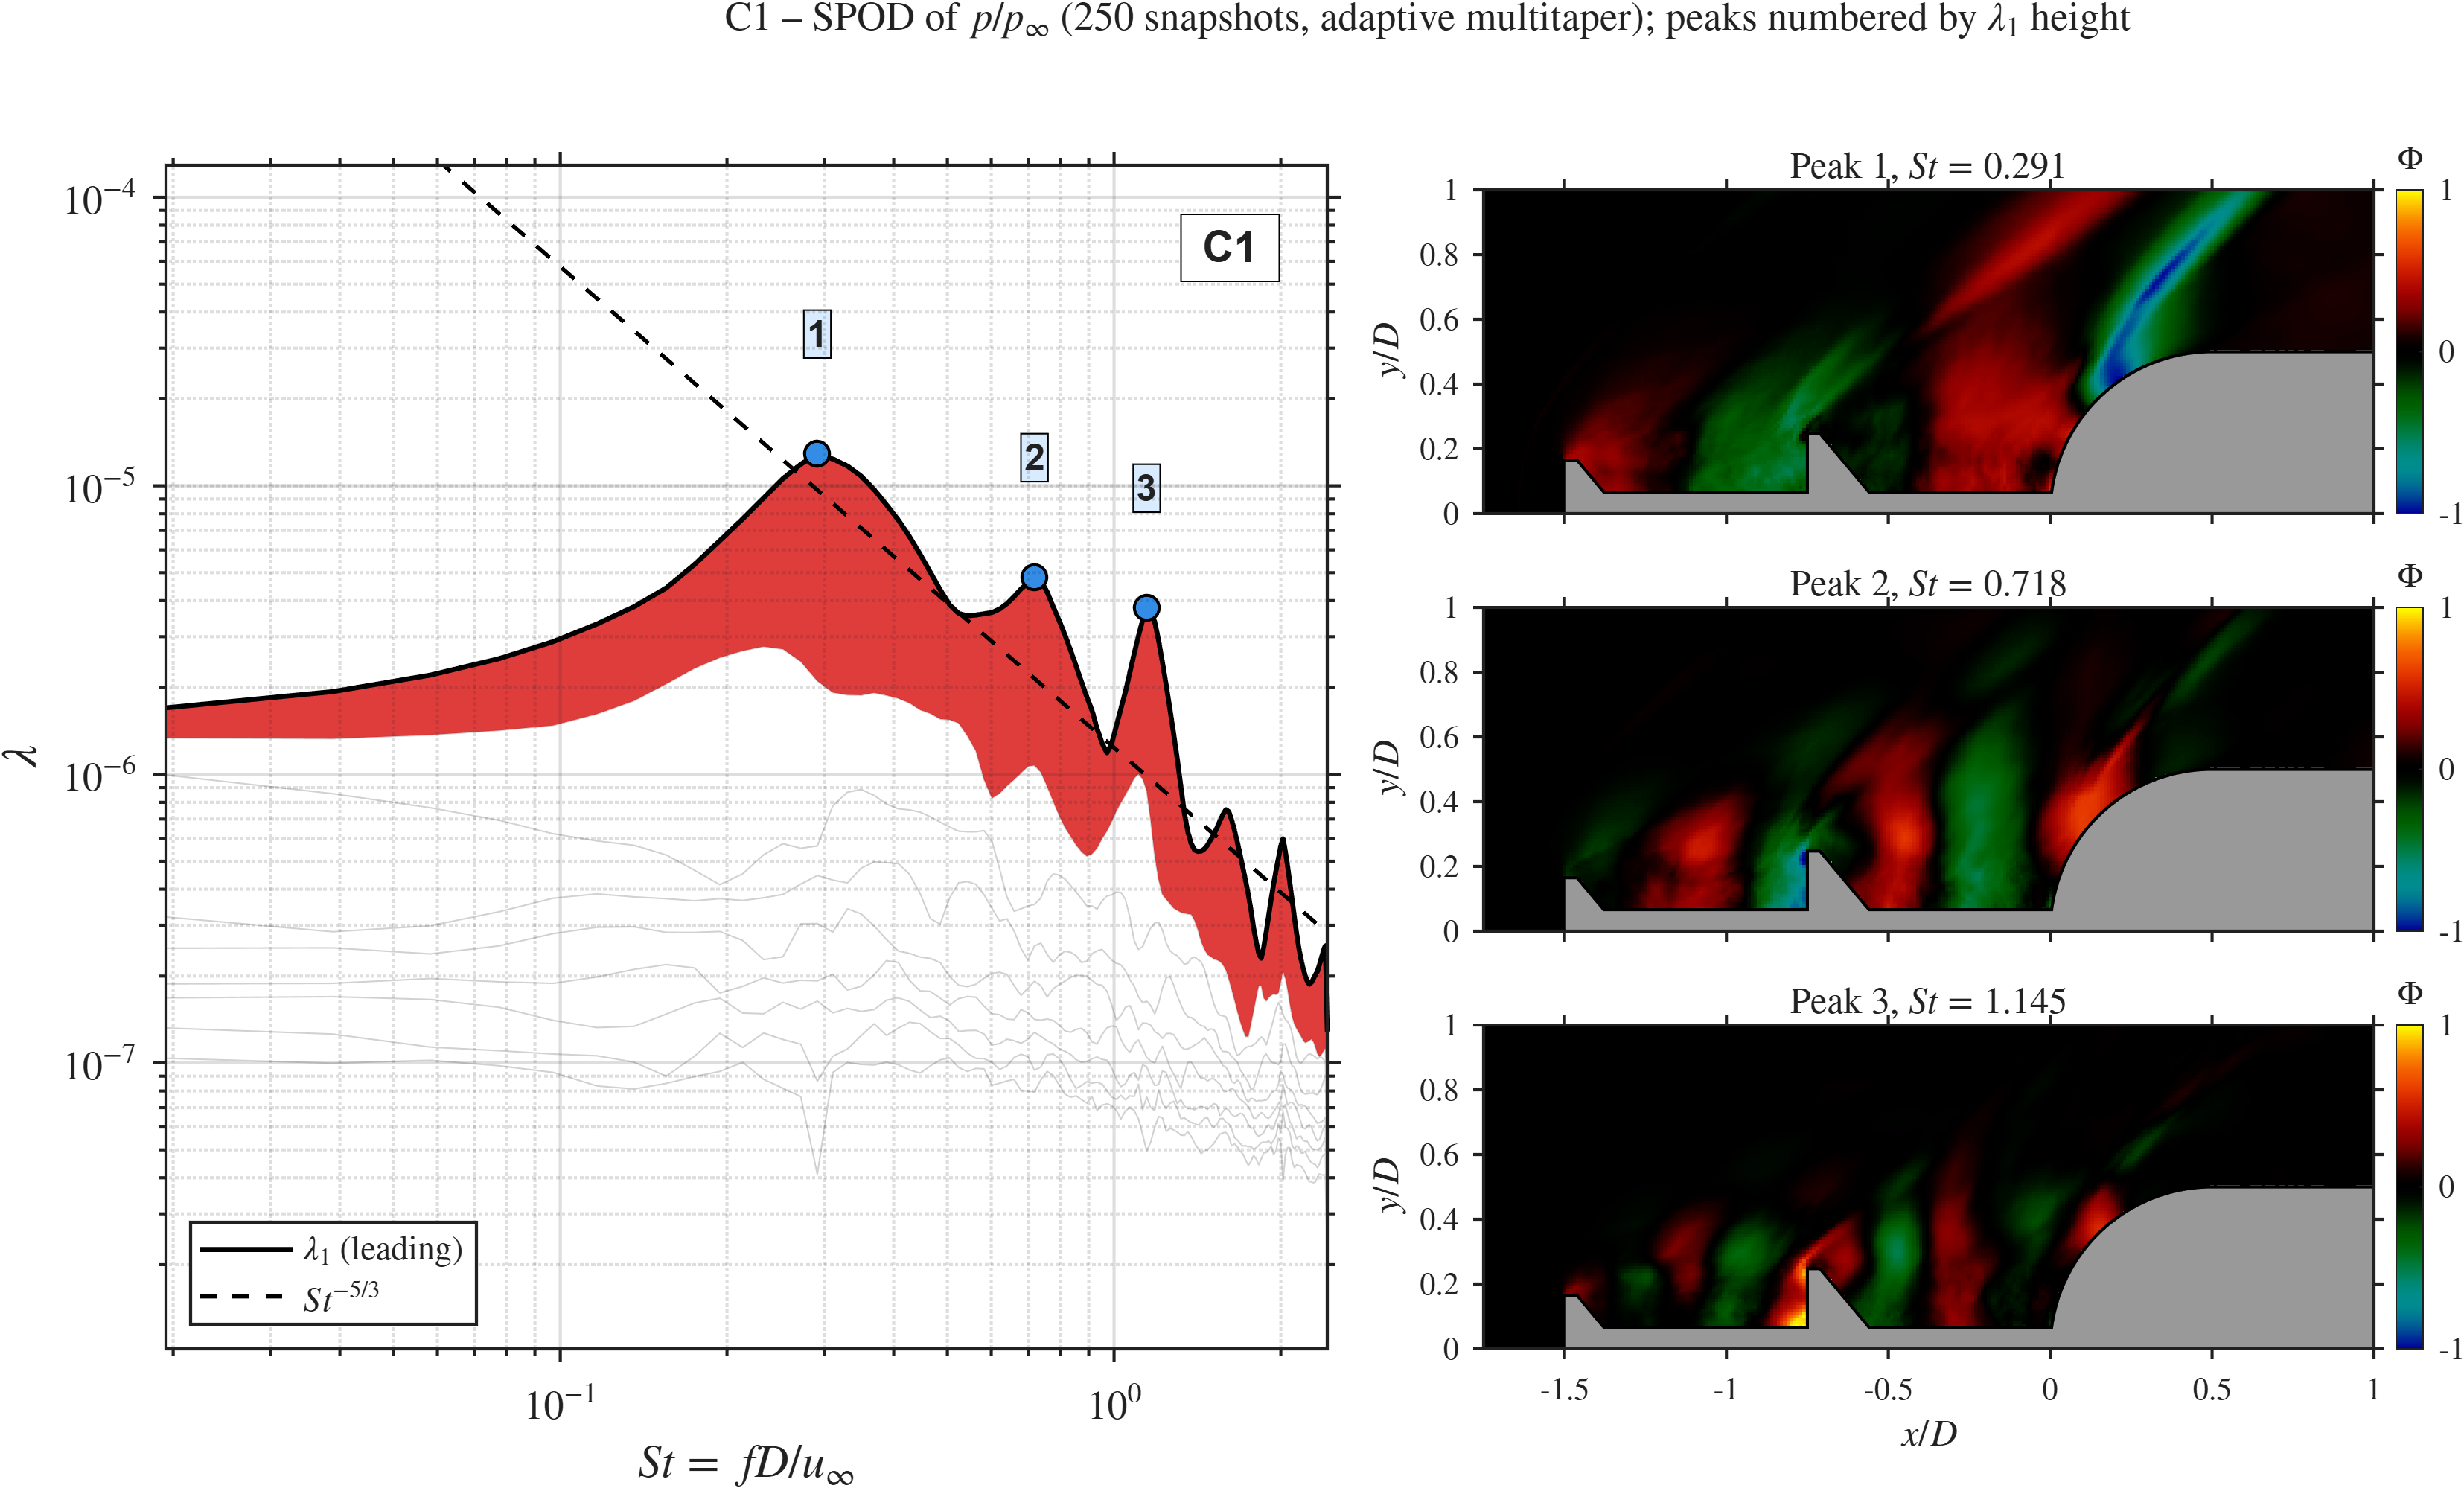
\includegraphics[width=\linewidth]{C1_spod.png}\caption{C1 ($l/D = 1.5$)}\end{subfigure}\\
  \begin{subfigure}{0.72\textwidth}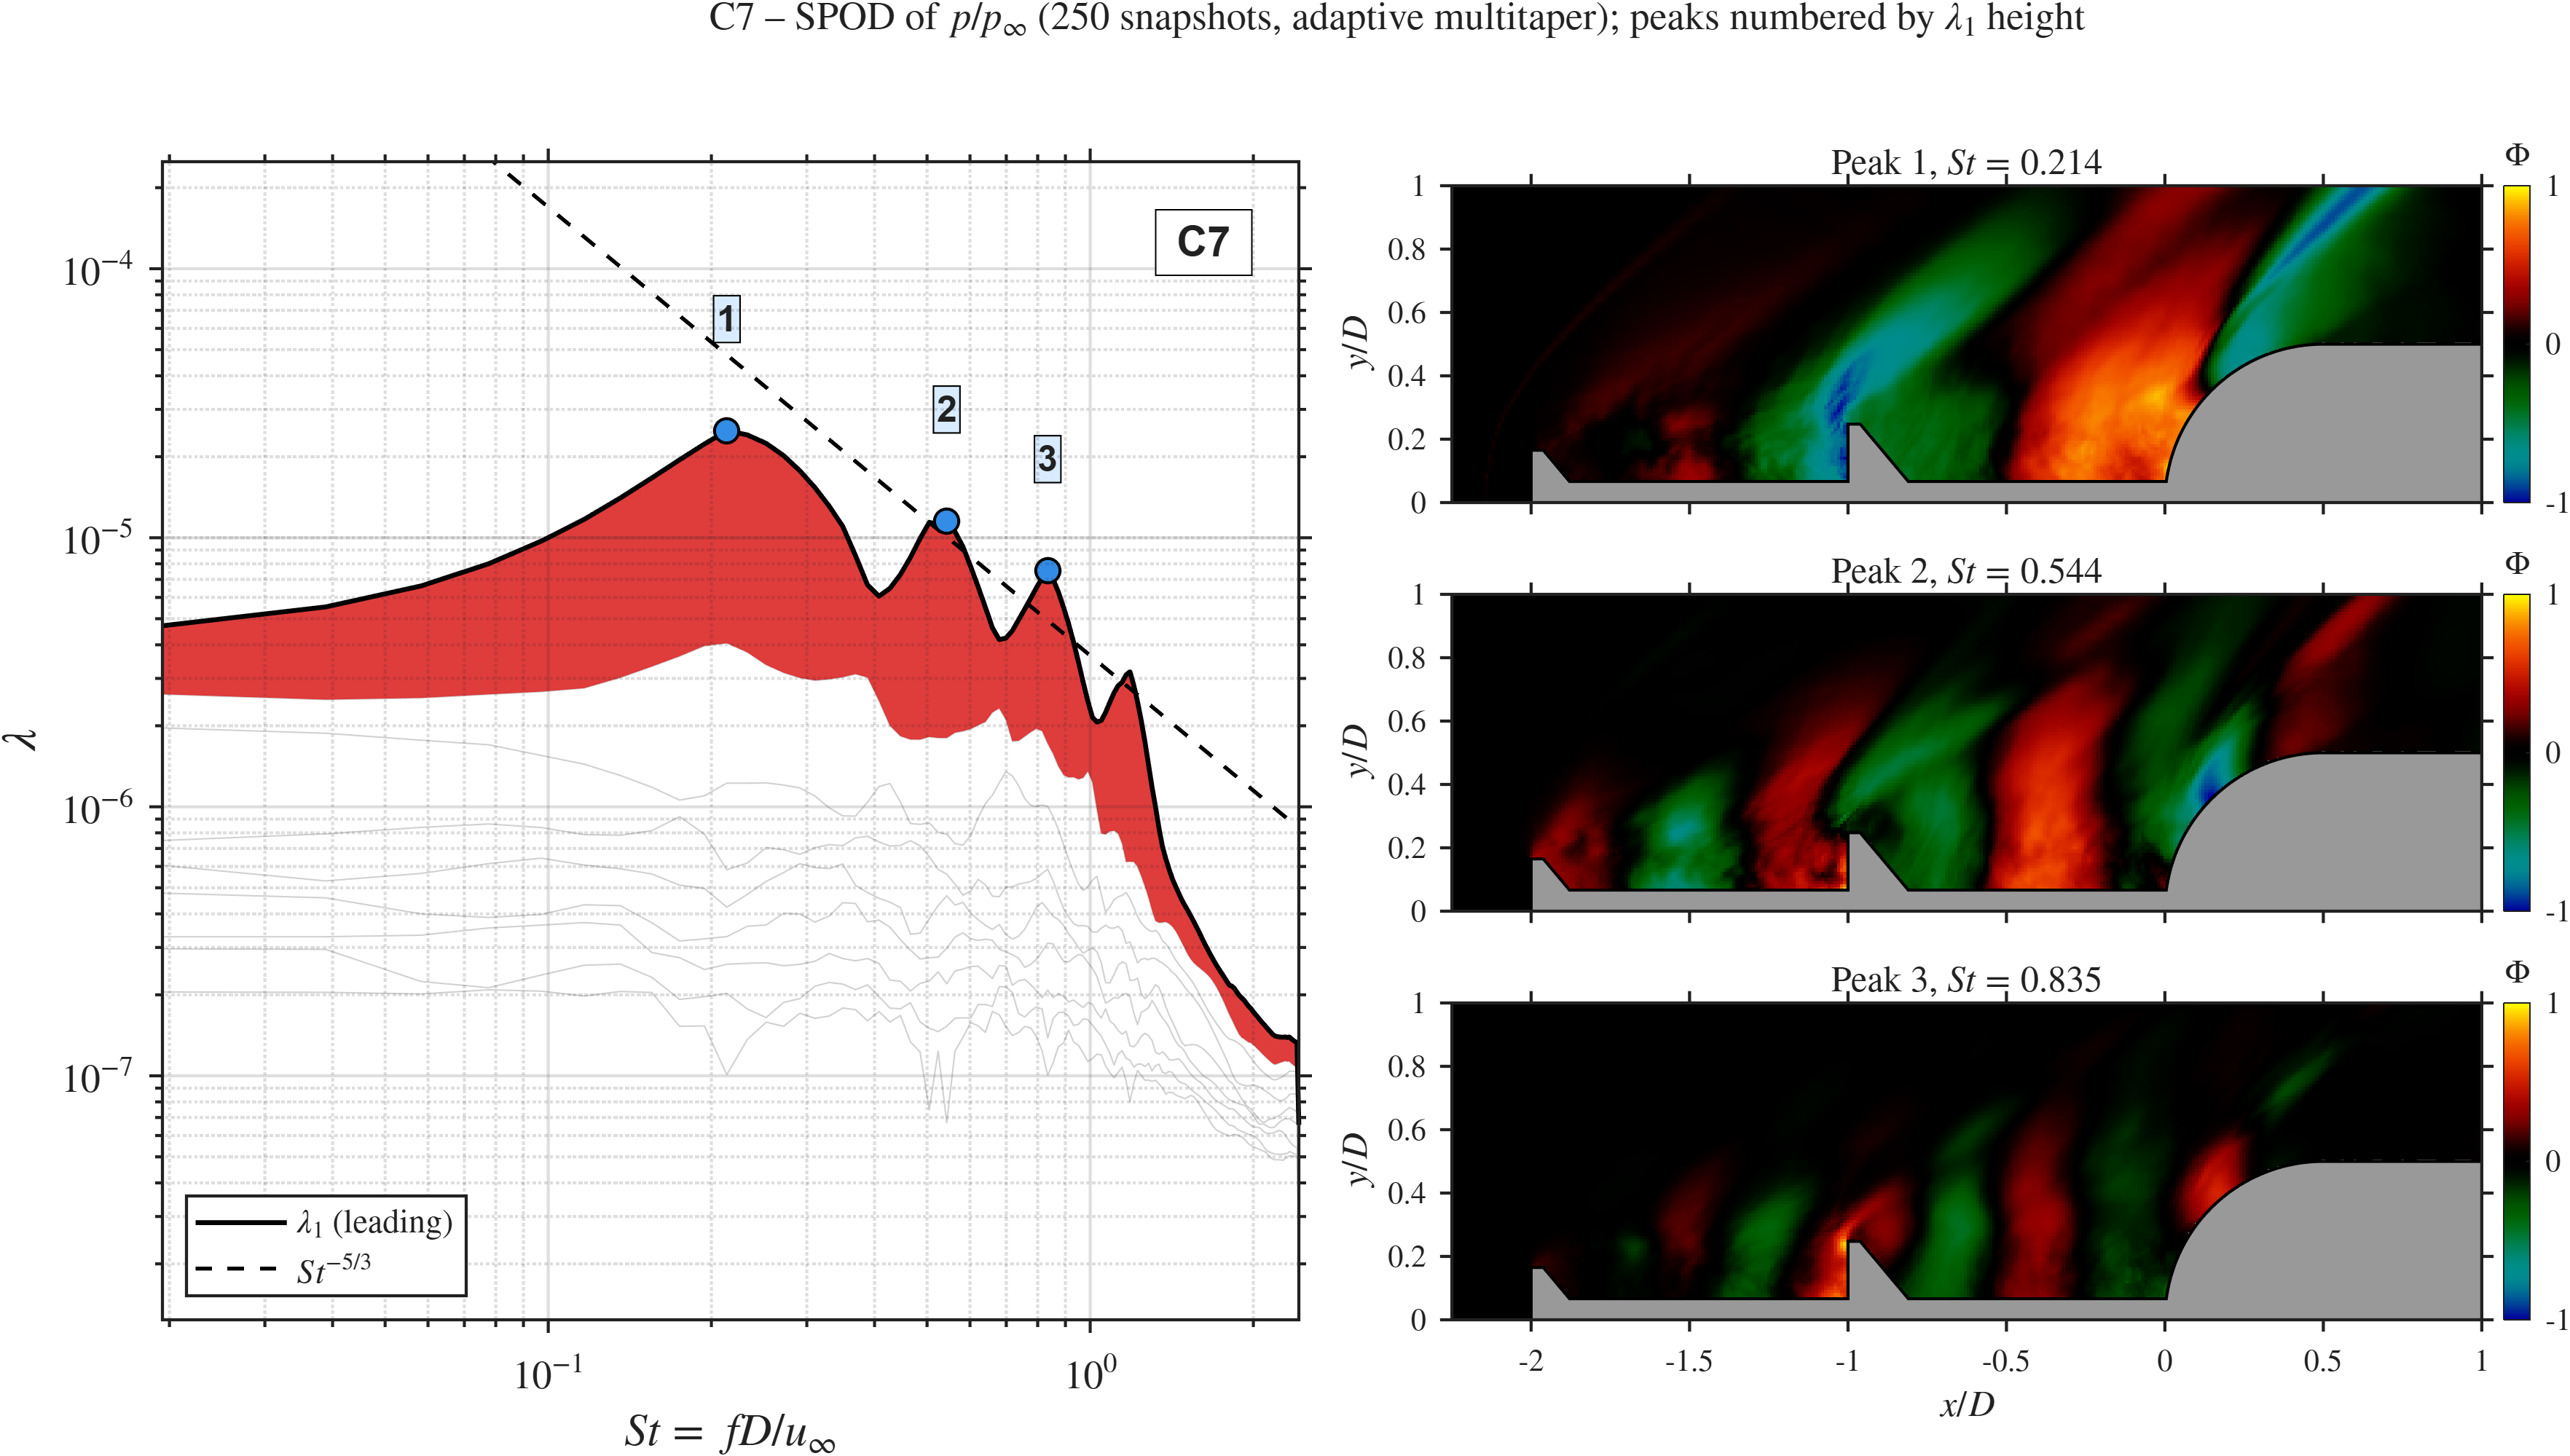
\includegraphics[width=\linewidth]{C7_spod.png}\caption{C7 ($l/D = 2$)}\end{subfigure}
  \caption{Spike-length sweep: SPOD spectra and leading modes.}
  \label{fig:len_spod}
\end{figure}

\paragraph{Summary.} Table~\ref{tab:len} lists the trends. This sweep gives the clearest monotonic trends. A longer spike lowers the shoulder pressure, with little further change beyond $l/D = 1.5$, and raises the drag fluctuation and $\lambda_1$ (the pressure fluctuation dips slightly at C6 and then rises). The mean drag has a shallow minimum at $l/D = 1.5$. C6 has the lowest drag fluctuation of all cases ($\sCd = 0.09$, below SA) but a 9.1\% higher shoulder pressure than C1. C7 gains little in mean pressure over C1 and has 33\% more drag fluctuation. Of the three lengths, $l/D = 1.5$ gives the best balance between mean load and unsteadiness.

\begin{table}[htbp]
  \centering
  \caption{Spike-length sweep. Percentages are relative to the pivot C1.}
  \label{tab:len}
  \begin{tabular}{lcccl}
    \toprule
    Metric & C6 ($l/D = 1$) & C1 ($l/D = 1.5$) & C7 ($l/D = 2$) & Trend with $l/D$ \\
    \midrule
    $\pbar$ & 2.03 ($+9.1\%$) & 1.86 & 1.83 ($-1.6\%$) & falls, levels off \\
    $\psd$ & 0.68 ($-6.8\%$) & 0.73 & 0.83 ($+13.7\%$) & rises \\
    $\Cdm$ & 0.40 ($+2.6\%$) & 0.39 & 0.41 ($+5.1\%$) & minimum at C1 \\
    $\sCd$ & 0.09 ($-25.0\%$) & 0.12 & 0.16 ($+33.3\%$) & rises \\
    $St$ peak, pressure & 1.13 & 1.12 & 0.82 & falls \\
    $St$ peak, drag & 1.12 & 1.14 & 0.82 & falls \\
    Peak $\Pi$ & $\approx 0.50$ & $\approx 0.37$ & $\approx 0.54$ & non-monotonic \\
    SPOD leading $St$ & 0.505 & 0.291 & 0.214 & falls \\
    SPOD peak $\lambda_1$ & $\approx 6\times10^{-6}$ & $\approx 1.3\times10^{-5}$ & $\approx 2.5\times10^{-5}$ & rises \\
    \bottomrule
  \end{tabular}
\end{table}

% ------------------------------------------------------------
\subsection{Comparison across all cases}\label{sec:synthesis}

Table~\ref{tab:master} collects the results of all eight cases.

\begin{table}[htbp]
  \centering
  \caption{All cases. Probe at $s/D \approx 0.4$. Percentages in brackets are relative to SA. $\Pi$ and $\lambda_1$ are read from the spectra.}
  \label{tab:master}
  \footnotesize
  \setlength{\tabcolsep}{2.5pt}
  \begin{tabular}{lccccccccccc}
    \toprule
    Case & $l/D$ & $\ltl$ & $\dtd$ & $\pbar$ & $\psd$ & $\Cdm$ & $\sCd$ & $St_p$ & $St_d$ & $\Pi$ & $\lambda_1$ ($St$) \\
    \midrule
    SA & 1.5 & -- & -- & 1.78 & 0.71 & 0.36 & 0.10 & 0.76 & 0.76 & 3.6 & $2.6\times10^{-5}$ (0.757) \\
    C1 & 1.5 & 1.0 & 1.5 & 1.86 ($+4.5$) & 0.73 ($+2.8$) & 0.39 ($+8.3$) & 0.12 ($+20$) & 1.12 & 1.14 & 0.37 & $1.3\times10^{-5}$ (0.291) \\
    C2 & 1.5 & 2.0 & 1.5 & 1.67 ($-6.2$) & 0.68 ($-4.2$) & 0.35 ($-2.8$) & 0.10 (0) & 0.56 & 0.89 & 0.50 & $8\times10^{-6}$ (0.524) \\
    C3 & 1.5 & 0.5 & 1.5 & 1.98 ($+11.2$) & 0.76 ($+7.0$) & 0.43 ($+19.4$) & 0.14 ($+40$) & 0.25 & 0.53 & 0.61 & $4\times10^{-5}$ (0.252) \\
    C4 & 1.5 & 1.0 & 1.0 & 2.12 ($+19.1$) & 0.87 ($+22.5$) & 0.41 ($+13.9$) & 0.11 ($+10$) & 0.83 & 0.83 & 0.72 & $1.4\times10^{-5}$ (0.835) \\
    C5 & 1.5 & 1.0 & 2.0 & 1.45 ($-18.5$) & 0.64 ($-9.9$) & 0.39 ($+8.3$) & 0.20 ($+100$) & 0.74 & 0.65 & 0.44 & $5.5\times10^{-5}$ (0.291) \\
    C6 & 1.0 & 1.0 & 1.5 & 2.03 ($+14.0$) & 0.68 ($-4.2$) & 0.40 ($+11.1$) & 0.09 ($-10$) & 1.13 & 1.12 & 0.50 & $6\times10^{-6}$ (0.505) \\
    C7 & 2.0 & 1.0 & 1.5 & 1.83 ($+2.8$) & 0.83 ($+16.9$) & 0.41 ($+13.9$) & 0.16 ($+60$) & 0.82 & 0.82 & 0.54 & $2.5\times10^{-5}$ (0.214) \\
    \bottomrule
  \end{tabular}
\end{table}

\paragraph{Which parameter matters most.} We compare the range of each metric within each sweep, with the other two parameters held at the pivot values. For the mean shoulder pressure, $\dtd$ gives the largest range (2.12 to 1.45, span 0.67), ahead of $\ltl$ (1.98 to 1.67, span 0.31) and $l/D$ (2.03 to 1.83, span 0.20). For the mean drag, $\ltl$ gives the largest range (0.43 to 0.35, span 0.08), while $\dtd$ and $l/D$ each span only 0.02. For the drag fluctuation, $\dtd$ gives the largest range (0.11 to 0.20, span 0.09), ahead of $l/D$ (0.09 to 0.16, span 0.07) and $\ltl$ (0.10 to 0.14, span 0.04), although $l/D$ gives the only monotonic trend. For the SPOD peak $\lambda_1$, $\dtd$ gives the largest range (span about $4.2\times10^{-5}$, mostly from C5), ahead of $\ltl$ (about $3.2\times10^{-5}$) and $l/D$ (about $1.9\times10^{-5}$). All DDAS cases lower the peak $\Pi$ by 80\% to 90\% relative to SA. No single parameter minimises every metric. In this matrix the gap ratio has the largest effect on mean drag, and the disk diameter ratio has the largest effect on mean shoulder pressure, drag fluctuation and coherent-mode energy.

\paragraph{Design trade-offs.} Two options stand out. For low mean drag and pressure, C2 ($\ltl = 2$) has the lowest $\Cdm$ (0.35) and the second-lowest $\pbar$ (1.67), with the same drag fluctuation as SA ($\sCd = 0.10$) and the second-lowest $\lambda_1$. The forward second disk makes Cavity 1 short and weakens the coupling between the cavities, so Cavity 2 acts almost as a single cavity. For low drag fluctuation, C6 ($l/D = 1$) has the lowest $\sCd$ (0.09, below SA) and the lowest $\lambda_1$, but the third-highest shoulder pressure (2.03). C5 ($\dtd = 2$) gives the largest cut in shoulder pressure ($-18.5\%$) but doubles the drag fluctuation of SA and carries the most energetic coherent mode, which would be a concern for fatigue loading.

\paragraph{Pressure and drag frequencies.} In SA, C1, C4, C6 and C7 the probe pressure and the drag peak at nearly the same $St$, so the shoulder pressure and the integrated drag follow one global mode. In C2, C3 and C5, where the gap or the disk size departs from the pivot, the two peaks differ by 12\% to 50\%. These geometries excite more than one mode with different spatial footprints: one that dominates the shoulder (probe $St$) and one that dominates the pressure over the disks and the forebody (drag $St$). In C3, for example, the drag peak matches the disk-face band of the $x$--$f$ diagram. A single shoulder probe is therefore not enough to estimate the frequency content of the drag in these cases.

% ------------------------------------------------------------
\subsection{Combined SPOD analysis}\label{sec:spod_all}

Table~\ref{tab:spod} ranks the eight cases by the peak of the leading SPOD eigenvalue.

\begin{table}[htbp]
  \centering
  \caption{SPOD leading-eigenvalue peak $\lambda_1$ and its $St$, ranked from highest to lowest. Values are read from the spectra.}
  \label{tab:spod}
  \begin{tabular}{clccl}
    \toprule
    Rank & Case & $St$ & $\lambda_1$ & Leading mode \\
    \midrule
    1 & C5 ($\dtd = 2$) & 0.291 & $\approx 5.5\times10^{-5}$ & two-cavity coupling, Cavity 1 and disk edge \\
    2 & C3 ($\ltl = 0.5$) & 0.252 & $\approx 4\times10^{-5}$ & cavity-wide pulsation, harmonic at $2St$ \\
    3 & SA & 0.757 & $\approx 2.6\times10^{-5}$ & single-tone global oscillation \\
    4 & C7 ($l/D = 2$) & 0.214 & $\approx 2.5\times10^{-5}$ & long global mode over the whole spike \\
    5 & C4 ($\dtd = 1$) & 0.835 & $\approx 1.4\times10^{-5}$ & SA-like single loop \\
    6 & C1 (pivot) & 0.291 & $\approx 1.3\times10^{-5}$ & two-cavity coupling \\
    7 & C2 ($\ltl = 2$) & 0.524 & $\approx 8\times10^{-6}$ & weak coupling, Cavity 2 \\
    8 & C6 ($l/D = 1$) & 0.505 & $\approx 6\times10^{-6}$ & compact, low energy \\
    \bottomrule
  \end{tabular}
\end{table}

SA ranks third in $\lambda_1$ even though it has by far the highest probe peak ($\Pi \approx 3.6$). The two measures differ: the SPOD eigenvalue is the variance of a mode integrated over the whole field, while $\Pi$ is the spectrum at one point. SA puts its energy into one narrow tone that is strongest near the shoulder, while C5 and C3 spread coherent energy over a larger area.

Across the DDAS cases, $\lambda_1$ varies about ninefold, from $6\times10^{-6}$ (C6) to $5.5\times10^{-5}$ (C5), so the geometry gives strong control over coherent-structure energy. The leading frequencies fall into two groups. Cases where the second disk sets up two-cavity coupling (C1, C3, C5, C7) have leading modes at $St \approx 0.21$ to 0.29, a low-frequency group linked to mass exchange between the cavities. Cases where the second disk does not split the flow (C4) or where the cavities are short or weakly coupled (C2, C6) have leading modes at $St \approx 0.5$ to 0.84, closer to the SA tone.

The leading modes take three shapes. Type I, a global oscillation (SA, C4), has large structures running from the disk along the shear layer to the shoulder with one dominant wavelength. Type II, a two-cavity coupling mode (C1, C3, C5, C7), has structures in both cavities, usually of opposite sign across the second disk, and a longer wavelength consistent with the lower $St$. This shape suggests that the cavities are coupled through the second disk, with mass exchange across the disk driving the slow oscillation. Type III, a compact confined mode (C2, C6), stays within one cavity (C2) or within the short two-cavity system (C6) and carries the least energy. Type II modes carry the most energy and appear when the second disk is large enough ($\dtd \ge 1.5$) and the cavities are long enough. They can be weakened by a shorter spike ($l/D = 1$) or a forward second disk ($\ltl = 2$). A smaller disk ($\dtd = 1$) also removes them, but the SA-type tonal mode returns.

% ============================================================
\section{Conclusions}\label{sec:conclusions}

We studied the unsteady flow over double-disk aerospikes on a hemisphere at $M_\infty = 2.01$ and $Re_D = 2.16\times10^6$ with 2D axisymmetric DDES. A single-disk baseline and seven DDAS cases, built around a pivot ($l/D = 1.5$, $\dtd = 1.5$, $\ltl = 1$), isolated the effects of the gap ratio, the disk diameter ratio and the spike length. The solver matched the Mach 2 experiment within 5.2\% in mean drag and 2.2 percentage points in $\kappa$.

\paragraph{RQ1, effect of the second disk.}
\begin{enumerate}
  \item SA has one tone at $St = 0.76$ with $\Pi \approx 3.6$. The pivot C1 spreads the energy over $St \approx 0.3$ to 2.5 and lowers the peak to $\Pi \approx 0.37$, about 90\% less.
  \item SPOD of C1 shows a new two-cavity mode at $St \approx 0.29$ and a disk-face mode at $St \approx 1.1$, while the SA-type mode remains, weaker, in Cavity 2.
  \item The second disk does not lower the mean load: the shoulder pressure rises by 4.5\% and the mean drag by 8.3\% relative to SA.
\end{enumerate}

\paragraph{RQ2, disk diameter ratio $\dtd$.}
\begin{enumerate}
  \item The mean shoulder pressure falls by 31.6\% from $\dtd = 1$ (C4, 2.12) to $\dtd = 2$ (C5, 1.45). C5 is 18.5\% below SA.
  \item The drag fluctuation rises by 82\% from C4 to C5. C5 has the highest $\sCd$ (0.20, twice SA) and the highest SPOD peak of all cases.
  \item C4 has the highest mean pressure and fluctuation level and keeps the SA-type single loop, so an equal-size second disk gives no benefit here.
  \item $\dtd = 1.5$ sets up the two-cavity mode with moderate drag fluctuation.
\end{enumerate}

\paragraph{RQ3, gap ratio $\ltl$.}
\begin{enumerate}
  \item From $\ltl = 0.5$ to 2, the mean drag falls by 18.6\% (0.43 to 0.35) and the SPOD peak falls about fivefold.
  \item At $\ltl = 0.5$ (C3) the short Cavity 2 gives a pulsation-like mode at $St = 0.25$ with a harmonic at twice that frequency.
  \item At $\ltl = 2$ (C2) the short Cavity 1 weakens the coupling and the flow moves toward SA-like behaviour. C2 has the lowest mean drag of all cases ($\Cdm = 0.35$, 2.8\% below SA) with the same drag fluctuation as SA, in line with our steady result for a forward second disk~\cite{Gujar2026staged}.
\end{enumerate}

\paragraph{RQ4, spike length $l/D$ and overall ranking.}
\begin{enumerate}
  \item A longer spike lowers the shoulder pressure, with little change beyond $l/D = 1.5$, and raises the drag fluctuation and the SPOD peak.
  \item C6 ($l/D = 1$) has the lowest drag fluctuation of all cases ($\sCd = 0.09$, below SA) but a 14\% higher shoulder pressure than SA. C7 ($l/D = 2$) gains little in mean pressure over C1 and has 33\% more drag fluctuation.
  \item The mean drag of the DDAS has a shallow minimum at $l/D = 1.5$ within the three lengths tested.
  \item No single parameter minimises all metrics. In this matrix the gap ratio has the largest effect on mean drag, and the disk diameter ratio has the largest effect on mean shoulder pressure, drag fluctuation and coherent-mode energy.
\end{enumerate}

\paragraph{Other findings.}
\begin{enumerate}
  \item In C2, C3 and C5 the probe and drag peak frequencies differ by 12\% to 50\%, so a single shoulder probe does not give the frequency content of the drag.
  \item The leading SPOD modes fall into three shapes: global single-cavity (SA, C4), two-cavity coupling (C1, C3, C5, C7, highest energy) and compact confined (C2, C6, lowest energy).
\end{enumerate}

\paragraph{Limitations and future work.} All results come from 2D axisymmetric DDES and should be read as relative trends between configurations. Azimuthal instabilities, spanwise vortex deformation and the 3D turbulent cascade are missing and may change the absolute drag and fluctuation levels. Wind-tunnel tests on DDAS models, and 3D DDES of selected cases, would test the trends found here, in particular the change from a tone to a broad band and the effect of $\ltl$ on the pulsation-like behaviour.

% ============================================================
\section*{Declaration of generative AI use}
The author used Claude (Anthropic) to edit the language of this report and to assemble the LaTeX source. The author reviewed and edited all text and takes full responsibility for the content.

\bibliographystyle{unsrtnat}
\bibliography{references}

\end{document}
